\documentclass[11pt]{report}

\usepackage[T1]{fontenc}
% Nicer default font (+ math font) than Computer Modern for most use cases
\usepackage{mathpazo}

% Basic figure setup, for now with no caption control since it's done
% automatically by Pandoc (which extracts ![](path) syntax from Markdown).
\usepackage{graphicx}
% We will generate all images so they have a width \maxwidth. This means
% that they will get their normal width if they fit onto the page, but
% are scaled down if they would overflow the margins.
\makeatletter
\def\maxwidth{\ifdim\Gin@nat@width>\linewidth\linewidth
\else\Gin@nat@width\fi}
\makeatother
\let\Oldincludegraphics\includegraphics
% Set max figure width to be 80% of text width, for now hardcoded.
\renewcommand{\includegraphics}[1]{\Oldincludegraphics[width=.8\maxwidth]{#1}}
% Ensure that by default, figures have no caption (until we provide a
% proper Figure object with a Caption API and a way to capture that
% in the conversion process - todo).
% \usepackage{caption}
% \DeclareCaptionLabelFormat{nolabel}{}
% \captionsetup{labelformat=nolabel}

\usepackage{adjustbox} % Used to constrain images to a maximum size 
\usepackage{xcolor} % Allow colors to be defined
\usepackage{enumerate} % Needed for markdown enumerations to work
\usepackage{geometry} % Used to adjust the document margins
\usepackage{amsmath} % Equations
\usepackage{amssymb} % Equations
\usepackage{textcomp} % defines textquotesingle
% Hack from http://tex.stackexchange.com/a/47451/13684:
\AtBeginDocument{%
    \def\PYZsq{\textquotesingle}% Upright quotes in Pygmentized code
}
\usepackage{upquote} % Upright quotes for verbatim code
\usepackage{eurosym} % defines \euro
\usepackage[mathletters]{ucs} % Extended unicode (utf-8) support
\usepackage[utf8x]{inputenc} % Allow utf-8 characters in the tex document
\usepackage{fancyvrb} % verbatim replacement that allows latex
\usepackage{grffile} % extends the file name processing of package graphics 
                     % to support a larger range 
% The hyperref package gives us a pdf with properly built
% internal navigation ('pdf bookmarks' for the table of contents,
% internal cross-reference links, web links for URLs, etc.)
\usepackage{hyperref}
\usepackage{longtable} % longtable support required by pandoc >1.10
\usepackage{booktabs}  % table support for pandoc > 1.12.2
\usepackage[normalem]{ulem} % ulem is needed to support strikethroughs (\sout)
                            % normalem makes italics be italics, not underlines

%\usepackage{ngerman}
\usepackage{fleqn}
\usepackage{epsfig}
\usepackage{a4wide}
\usepackage{amssymb}
\usepackage{wasysym}
\usepackage{stmaryrd}
\usepackage{color}
\usepackage{alltt}
\usepackage{theorem}
\usepackage{minted}
\usepackage{makeidx}

\usepackage{hyperref}
\usepackage[all]{hypcap}
\hypersetup{
  colorlinks = true, 
  linkcolor  = blue,
  citecolor  = red,
  filecolor  = Gold,
  urlcolor   = [rgb]{0.5, 0.0, 0.5},
  pdfborder  = {0 0 0} 
}

\usepackage{fancyhdr}
\usepackage{lastpage} 


% Colors for the hyperref package
\definecolor{urlcolor}{rgb}{0.5,0,0.5}
\definecolor{linkcolor}{rgb}{0.0,0.0,1.0}
\definecolor{citecolor}{rgb}{.12,.54,.11}
\definecolor{ttcolor}{rgb}{0.4,0.1,0.0}

% ANSI colors
\definecolor{ansi-black}{HTML}{3E424D}
\definecolor{ansi-black-intense}{HTML}{282C36}
\definecolor{ansi-red}{HTML}{E75C58}
\definecolor{ansi-red-intense}{HTML}{B22B31}
\definecolor{ansi-green}{HTML}{00A250}
\definecolor{ansi-green-intense}{HTML}{007427}
\definecolor{ansi-yellow}{HTML}{DDB62B}
\definecolor{ansi-yellow-intense}{HTML}{B27D12}
\definecolor{ansi-blue}{HTML}{208FFB}
\definecolor{ansi-blue-intense}{HTML}{0065CA}
\definecolor{ansi-magenta}{HTML}{D160C4}
\definecolor{ansi-magenta-intense}{HTML}{A03196}
\definecolor{ansi-cyan}{HTML}{60C6C8}
\definecolor{ansi-cyan-intense}{HTML}{258F8F}
\definecolor{ansi-white}{HTML}{C5C1B4}
\definecolor{ansi-white-intense}{HTML}{A1A6B2}

% commands and environments needed by pandoc snippets
% extracted from the output of `pandoc -s`
\providecommand{\tightlist}{%
  \setlength{\itemsep}{0pt}\setlength{\parskip}{0pt}}
\DefineVerbatimEnvironment{Highlighting}{Verbatim}{commandchars=\\\{\}}
% Add ',fontsize=\small' for more characters per line
\newenvironment{Shaded}{}{}
\newcommand{\KeywordTok}[1]{\textcolor[rgb]{0.00,0.44,0.13}{\textbf{{#1}}}}
\newcommand{\DataTypeTok}[1]{\textcolor[rgb]{0.56,0.13,0.00}{{#1}}}
\newcommand{\DecValTok}[1]{\textcolor[rgb]{0.25,0.63,0.44}{{#1}}}
\newcommand{\BaseNTok}[1]{\textcolor[rgb]{0.25,0.63,0.44}{{#1}}}
\newcommand{\FloatTok}[1]{\textcolor[rgb]{0.25,0.63,0.44}{{#1}}}
\newcommand{\CharTok}[1]{\textcolor[rgb]{0.25,0.44,0.63}{{#1}}}
\newcommand{\StringTok}[1]{\textcolor[rgb]{0.25,0.44,0.63}{{#1}}}
\newcommand{\CommentTok}[1]{\textcolor[rgb]{0.38,0.63,0.69}{\textit{{#1}}}}
\newcommand{\OtherTok}[1]{\textcolor[rgb]{0.00,0.44,0.13}{{#1}}}
\newcommand{\AlertTok}[1]{\textcolor[rgb]{1.00,0.00,0.00}{\textbf{{#1}}}}
\newcommand{\FunctionTok}[1]{\textcolor[rgb]{0.02,0.16,0.49}{{#1}}}
\newcommand{\RegionMarkerTok}[1]{{#1}}
\newcommand{\ErrorTok}[1]{\textcolor[rgb]{1.00,0.00,0.00}{\textbf{{#1}}}}
\newcommand{\NormalTok}[1]{{#1}}

% Additional commands for more recent versions of Pandoc
\newcommand{\ConstantTok}[1]{\textcolor[rgb]{0.53,0.00,0.00}{{#1}}}
\newcommand{\SpecialCharTok}[1]{\textcolor[rgb]{0.25,0.44,0.63}{{#1}}}
\newcommand{\VerbatimStringTok}[1]{\textcolor[rgb]{0.25,0.44,0.63}{{#1}}}
\newcommand{\SpecialStringTok}[1]{\textcolor[rgb]{0.73,0.40,0.53}{{#1}}}
\newcommand{\ImportTok}[1]{{#1}}
\newcommand{\DocumentationTok}[1]{\textcolor[rgb]{0.73,0.13,0.13}{\textit{{#1}}}}
\newcommand{\AnnotationTok}[1]{\textcolor[rgb]{0.38,0.63,0.69}{\textbf{\textit{{#1}}}}}
\newcommand{\CommentVarTok}[1]{\textcolor[rgb]{0.38,0.63,0.69}{\textbf{\textit{{#1}}}}}
\newcommand{\VariableTok}[1]{\textcolor[rgb]{0.10,0.09,0.49}{{#1}}}
\newcommand{\ControlFlowTok}[1]{\textcolor[rgb]{0.00,0.44,0.13}{\textbf{{#1}}}}
\newcommand{\OperatorTok}[1]{\textcolor[rgb]{0.40,0.40,0.40}{{#1}}}
\newcommand{\BuiltInTok}[1]{{#1}}
\newcommand{\ExtensionTok}[1]{{#1}}
\newcommand{\PreprocessorTok}[1]{\textcolor[rgb]{0.74,0.48,0.00}{{#1}}}
\newcommand{\AttributeTok}[1]{\textcolor[rgb]{0.49,0.56,0.16}{{#1}}}
\newcommand{\InformationTok}[1]{\textcolor[rgb]{0.38,0.63,0.69}{\textbf{\textit{{#1}}}}}
\newcommand{\WarningTok}[1]{\textcolor[rgb]{0.38,0.63,0.69}{\textbf{\textit{{#1}}}}}


% Define a nice break command that doesn't care if a line doesn't already
% exist.
\def\br{\hspace*{\fill} \\* }
% Math Jax compatability definitions
\def\gt{>}
\def\lt{<}
% Document parameters
\title{Introduction}

% Pygments definitions
    
\makeatletter
\def\PY@reset{\let\PY@it=\relax \let\PY@bf=\relax%
    \let\PY@ul=\relax \let\PY@tc=\relax%
    \let\PY@bc=\relax \let\PY@ff=\relax}
\def\PY@tok#1{\csname PY@tok@#1\endcsname}
\def\PY@toks#1+{\ifx\relax#1\empty\else%
    \PY@tok{#1}\expandafter\PY@toks\fi}
\def\PY@do#1{\PY@bc{\PY@tc{\PY@ul{%
    \PY@it{\PY@bf{\PY@ff{#1}}}}}}}
\def\PY#1#2{\PY@reset\PY@toks#1+\relax+\PY@do{#2}}

\expandafter\def\csname PY@tok@w\endcsname{\def\PY@tc##1{\textcolor[rgb]{0.73,0.73,0.73}{##1}}}
\expandafter\def\csname PY@tok@c\endcsname{\let\PY@it=\textit\def\PY@tc##1{\textcolor[rgb]{0.25,0.50,0.50}{##1}}}
\expandafter\def\csname PY@tok@cp\endcsname{\def\PY@tc##1{\textcolor[rgb]{0.74,0.48,0.00}{##1}}}
\expandafter\def\csname PY@tok@k\endcsname{\let\PY@bf=\textbf\def\PY@tc##1{\textcolor[rgb]{0.00,0.50,0.00}{##1}}}
\expandafter\def\csname PY@tok@kp\endcsname{\def\PY@tc##1{\textcolor[rgb]{0.00,0.50,0.00}{##1}}}
\expandafter\def\csname PY@tok@kt\endcsname{\def\PY@tc##1{\textcolor[rgb]{0.69,0.00,0.25}{##1}}}
\expandafter\def\csname PY@tok@o\endcsname{\def\PY@tc##1{\textcolor[rgb]{0.40,0.40,0.40}{##1}}}
\expandafter\def\csname PY@tok@ow\endcsname{\let\PY@bf=\textbf\def\PY@tc##1{\textcolor[rgb]{0.67,0.13,1.00}{##1}}}
\expandafter\def\csname PY@tok@nb\endcsname{\def\PY@tc##1{\textcolor[rgb]{0.00,0.50,0.00}{##1}}}
\expandafter\def\csname PY@tok@nf\endcsname{\def\PY@tc##1{\textcolor[rgb]{0.00,0.00,1.00}{##1}}}
\expandafter\def\csname PY@tok@nc\endcsname{\let\PY@bf=\textbf\def\PY@tc##1{\textcolor[rgb]{0.00,0.00,1.00}{##1}}}
\expandafter\def\csname PY@tok@nn\endcsname{\let\PY@bf=\textbf\def\PY@tc##1{\textcolor[rgb]{0.00,0.00,1.00}{##1}}}
\expandafter\def\csname PY@tok@ne\endcsname{\let\PY@bf=\textbf\def\PY@tc##1{\textcolor[rgb]{0.82,0.25,0.23}{##1}}}
\expandafter\def\csname PY@tok@nv\endcsname{\def\PY@tc##1{\textcolor[rgb]{0.10,0.09,0.49}{##1}}}
\expandafter\def\csname PY@tok@no\endcsname{\def\PY@tc##1{\textcolor[rgb]{0.53,0.00,0.00}{##1}}}
\expandafter\def\csname PY@tok@nl\endcsname{\def\PY@tc##1{\textcolor[rgb]{0.63,0.63,0.00}{##1}}}
\expandafter\def\csname PY@tok@ni\endcsname{\let\PY@bf=\textbf\def\PY@tc##1{\textcolor[rgb]{0.60,0.60,0.60}{##1}}}
\expandafter\def\csname PY@tok@na\endcsname{\def\PY@tc##1{\textcolor[rgb]{0.49,0.56,0.16}{##1}}}
\expandafter\def\csname PY@tok@nt\endcsname{\let\PY@bf=\textbf\def\PY@tc##1{\textcolor[rgb]{0.00,0.50,0.00}{##1}}}
\expandafter\def\csname PY@tok@nd\endcsname{\def\PY@tc##1{\textcolor[rgb]{0.67,0.13,1.00}{##1}}}
\expandafter\def\csname PY@tok@s\endcsname{\def\PY@tc##1{\textcolor[rgb]{0.73,0.13,0.13}{##1}}}
\expandafter\def\csname PY@tok@sd\endcsname{\let\PY@it=\textit\def\PY@tc##1{\textcolor[rgb]{0.73,0.13,0.13}{##1}}}
\expandafter\def\csname PY@tok@si\endcsname{\let\PY@bf=\textbf\def\PY@tc##1{\textcolor[rgb]{0.73,0.40,0.53}{##1}}}
\expandafter\def\csname PY@tok@se\endcsname{\let\PY@bf=\textbf\def\PY@tc##1{\textcolor[rgb]{0.73,0.40,0.13}{##1}}}
\expandafter\def\csname PY@tok@sr\endcsname{\def\PY@tc##1{\textcolor[rgb]{0.73,0.40,0.53}{##1}}}
\expandafter\def\csname PY@tok@ss\endcsname{\def\PY@tc##1{\textcolor[rgb]{0.10,0.09,0.49}{##1}}}
\expandafter\def\csname PY@tok@sx\endcsname{\def\PY@tc##1{\textcolor[rgb]{0.00,0.50,0.00}{##1}}}
\expandafter\def\csname PY@tok@m\endcsname{\def\PY@tc##1{\textcolor[rgb]{0.40,0.40,0.40}{##1}}}
\expandafter\def\csname PY@tok@gh\endcsname{\let\PY@bf=\textbf\def\PY@tc##1{\textcolor[rgb]{0.00,0.00,0.50}{##1}}}
\expandafter\def\csname PY@tok@gu\endcsname{\let\PY@bf=\textbf\def\PY@tc##1{\textcolor[rgb]{0.50,0.00,0.50}{##1}}}
\expandafter\def\csname PY@tok@gd\endcsname{\def\PY@tc##1{\textcolor[rgb]{0.63,0.00,0.00}{##1}}}
\expandafter\def\csname PY@tok@gi\endcsname{\def\PY@tc##1{\textcolor[rgb]{0.00,0.63,0.00}{##1}}}
\expandafter\def\csname PY@tok@gr\endcsname{\def\PY@tc##1{\textcolor[rgb]{1.00,0.00,0.00}{##1}}}
\expandafter\def\csname PY@tok@ge\endcsname{\let\PY@it=\textit}
\expandafter\def\csname PY@tok@gs\endcsname{\let\PY@bf=\textbf}
\expandafter\def\csname PY@tok@gp\endcsname{\let\PY@bf=\textbf\def\PY@tc##1{\textcolor[rgb]{0.00,0.00,0.50}{##1}}}
\expandafter\def\csname PY@tok@go\endcsname{\def\PY@tc##1{\textcolor[rgb]{0.53,0.53,0.53}{##1}}}
\expandafter\def\csname PY@tok@gt\endcsname{\def\PY@tc##1{\textcolor[rgb]{0.00,0.27,0.87}{##1}}}
\expandafter\def\csname PY@tok@err\endcsname{\def\PY@bc##1{\setlength{\fboxsep}{0pt}\fcolorbox[rgb]{1.00,0.00,0.00}{1,1,1}{\strut ##1}}}
\expandafter\def\csname PY@tok@kc\endcsname{\let\PY@bf=\textbf\def\PY@tc##1{\textcolor[rgb]{0.00,0.50,0.00}{##1}}}
\expandafter\def\csname PY@tok@kd\endcsname{\let\PY@bf=\textbf\def\PY@tc##1{\textcolor[rgb]{0.00,0.50,0.00}{##1}}}
\expandafter\def\csname PY@tok@kn\endcsname{\let\PY@bf=\textbf\def\PY@tc##1{\textcolor[rgb]{0.00,0.50,0.00}{##1}}}
\expandafter\def\csname PY@tok@kr\endcsname{\let\PY@bf=\textbf\def\PY@tc##1{\textcolor[rgb]{0.00,0.50,0.00}{##1}}}
\expandafter\def\csname PY@tok@bp\endcsname{\def\PY@tc##1{\textcolor[rgb]{0.00,0.50,0.00}{##1}}}
\expandafter\def\csname PY@tok@fm\endcsname{\def\PY@tc##1{\textcolor[rgb]{0.00,0.00,1.00}{##1}}}
\expandafter\def\csname PY@tok@vc\endcsname{\def\PY@tc##1{\textcolor[rgb]{0.10,0.09,0.49}{##1}}}
\expandafter\def\csname PY@tok@vg\endcsname{\def\PY@tc##1{\textcolor[rgb]{0.10,0.09,0.49}{##1}}}
\expandafter\def\csname PY@tok@vi\endcsname{\def\PY@tc##1{\textcolor[rgb]{0.10,0.09,0.49}{##1}}}
\expandafter\def\csname PY@tok@vm\endcsname{\def\PY@tc##1{\textcolor[rgb]{0.10,0.09,0.49}{##1}}}
\expandafter\def\csname PY@tok@sa\endcsname{\def\PY@tc##1{\textcolor[rgb]{0.73,0.13,0.13}{##1}}}
\expandafter\def\csname PY@tok@sb\endcsname{\def\PY@tc##1{\textcolor[rgb]{0.73,0.13,0.13}{##1}}}
\expandafter\def\csname PY@tok@sc\endcsname{\def\PY@tc##1{\textcolor[rgb]{0.73,0.13,0.13}{##1}}}
\expandafter\def\csname PY@tok@dl\endcsname{\def\PY@tc##1{\textcolor[rgb]{0.73,0.13,0.13}{##1}}}
\expandafter\def\csname PY@tok@s2\endcsname{\def\PY@tc##1{\textcolor[rgb]{0.73,0.13,0.13}{##1}}}
\expandafter\def\csname PY@tok@sh\endcsname{\def\PY@tc##1{\textcolor[rgb]{0.73,0.13,0.13}{##1}}}
\expandafter\def\csname PY@tok@s1\endcsname{\def\PY@tc##1{\textcolor[rgb]{0.73,0.13,0.13}{##1}}}
\expandafter\def\csname PY@tok@mb\endcsname{\def\PY@tc##1{\textcolor[rgb]{0.40,0.40,0.40}{##1}}}
\expandafter\def\csname PY@tok@mf\endcsname{\def\PY@tc##1{\textcolor[rgb]{0.40,0.40,0.40}{##1}}}
\expandafter\def\csname PY@tok@mh\endcsname{\def\PY@tc##1{\textcolor[rgb]{0.40,0.40,0.40}{##1}}}
\expandafter\def\csname PY@tok@mi\endcsname{\def\PY@tc##1{\textcolor[rgb]{0.40,0.40,0.40}{##1}}}
\expandafter\def\csname PY@tok@il\endcsname{\def\PY@tc##1{\textcolor[rgb]{0.40,0.40,0.40}{##1}}}
\expandafter\def\csname PY@tok@mo\endcsname{\def\PY@tc##1{\textcolor[rgb]{0.40,0.40,0.40}{##1}}}
\expandafter\def\csname PY@tok@ch\endcsname{\let\PY@it=\textit\def\PY@tc##1{\textcolor[rgb]{0.25,0.50,0.50}{##1}}}
\expandafter\def\csname PY@tok@cm\endcsname{\let\PY@it=\textit\def\PY@tc##1{\textcolor[rgb]{0.25,0.50,0.50}{##1}}}
\expandafter\def\csname PY@tok@cpf\endcsname{\let\PY@it=\textit\def\PY@tc##1{\textcolor[rgb]{0.25,0.50,0.50}{##1}}}
\expandafter\def\csname PY@tok@c1\endcsname{\let\PY@it=\textit\def\PY@tc##1{\textcolor[rgb]{0.25,0.50,0.50}{##1}}}
\expandafter\def\csname PY@tok@cs\endcsname{\let\PY@it=\textit\def\PY@tc##1{\textcolor[rgb]{0.25,0.50,0.50}{##1}}}

\def\PYZbs{\char`\\}
\def\PYZus{\char`\_}
\def\PYZob{\char`\{}
\def\PYZcb{\char`\}}
\def\PYZca{\char`\^}
\def\PYZam{\char`\&}
\def\PYZlt{\char`\<}
\def\PYZgt{\char`\>}
\def\PYZsh{\char`\#}
\def\PYZpc{\char`\%}
\def\PYZdl{\char`\$} %$
\def\PYZhy{\char`\-}
\def\PYZsq{\char`\'}
\def\PYZdq{\char`\"}
\def\PYZti{\char`\~}
% for compatibility with earlier versions
\def\PYZat{@}
\def\PYZlb{[}
\def\PYZrb{]}
\makeatother


    % Exact colors from NB
    \definecolor{incolor}{rgb}{0.0, 0.0, 0.5}
    \definecolor{outcolor}{rgb}{0.545, 0.0, 0.0}



    
    % Prevent overflowing lines due to hard-to-break entities
    \sloppy 
    % Setup hyperref package
    \hypersetup{
      breaklinks=true,  % so long urls are correctly broken across lines
      colorlinks=true,
      urlcolor=urlcolor,
      linkcolor=linkcolor,
      citecolor=citecolor,
      }
    % Slightly bigger margins than the latex defaults
    
    \geometry{verbose,tmargin=1in,bmargin=1in,lmargin=1in,rmargin=1in}
    


% Stick with serif fonts, so that monospace font look different from normal text. 
%\renewcommand*{\familydefault}{\sfdefault}

\newcommand{\blue}[1]{{\color{blue}#1}}
\newcommand{\red}[1]{{\color{red}#1}}
\newcommand{\mytt}[1]{{\color{ttcolor}\texttt{#1}}}
\pagestyle{fancy}

\fancyfoot[C]{--- \thepage/\pageref{LastPage}\ ---}

\fancypagestyle{plain}{%
\fancyhf{}
\fancyfoot[C]{--- \thepage/\pageref{LastPage}\ ---}
\renewcommand{\headrulewidth}{0pt}
}

\fancyheadoffset{0.1cm}
\renewcommand{\chaptermark}[1]{\markboth{\chaptername \ \thechapter.\ #1}{}}
\renewcommand{\sectionmark}[1]{\markright{\thesection. \ #1}{}}
\fancyhead[R]{\leftmark}
\fancyhead[L]{\rightmark}

\definecolor{amethyst}{rgb}{1.0, 0.7, 0.4}
\definecolor{orange}{rgb}{1, 0.9, 0.0}
\definecolor{sepia}{rgb}{1.0,1.0,0.9}

\setlength{\mathindent}{1.3cm}
\setlength{\textwidth}{17cm}
\addtolength{\oddsidemargin}{-1cm}
\addtolength{\evensidemargin}{-1cm}
\addtolength{\topmargin}{-1cm}


\setlength{\mathindent}{1.3cm}
\setlength{\topsep}{0.1cm plus0.1cm minus 0.0cm}
\setlength{\partopsep}{0.0cm plus0.1cm minus 0.0cm}
\setlength{\parsep}{0.1cm plus0.1cm minus 0.0cm}
\setlength{\parskip}{0.1cm plus0.1cm minus 0.0cm}
\newfont{\chess}{chess20}
\newfont{\bigchess}{chess30}
\newcommand{\chf}{\baselineskip20pt\lineskip0pt\chess}
\newcommand{\ds}{\displaystyle}
\newcommand{\diff}{\frac{\textrm{d}\;\;}{\textrm{d}\mbox{$x$}}}

{\theorembodyfont{\slshape}
\newtheorem{Definition}{Definition}
\newtheorem{Notation}[Definition]{Notation}
\newtheorem{Korollar}[Definition]{Korollar}
\newtheorem{Lemma}[Definition]{Lemma}
\newtheorem{Satz}[Definition]{Satz}
\newtheorem{Theorem}[Definition]{Theorem}
}

\hyphenation{com-pre-hen-sion}
% set the monospace-font to Inconsalata-g
% font-source: http://leonardo-m.livejournal.com/77079.html

\title{\epsfig{file=dhbw-logo.eps, scale=1.2}  \\[0.2cm]
       Theoretical Computer Science \texttt{I}: \\
       An Introduction to Logic via \textsl{Python} \\[0.3cm]
      --- Autumn 2020 ---     \\[0.3cm]
      Baden-Wuerttemberg Cooperative State University (DHBW)}
\author{Prof.~Dr.~Karl Stroetmann}


\date{\today \\[0.5cm]
\begin{minipage}[t]{1.0\linewidth}
\noindent
These lecture notes, the corresponding \LaTeX\ sources and the programs discussed in these lecture notes are available at
\\[0.2cm]
\hspace*{\fill}
\href{https://github.com/karlstroetmann/Logic}{\texttt{https://github.com/karlstroetmann/Logic}}.
\hspace*{\fill} 
\\[0.2cm]
The \href{https://github.com/karlstroetmann/Logic/blob/master/Lecture-Notes/logic.pdf}{lecture notes}
can be found in the directory
\href{https://github.com/karlstroetmann/Logic/blob/master/Lecture-Notes}{\texttt{Lecture-Notes}}
in the file
\href{https://github.com/karlstroetmann/Logic/blob/master/Lecture-Notes/logic.pdf}{\texttt{logic.pdf}}.
The \href{https://jupyter-notebook.readthedocs.io/en/stable/}{Jupyter Notebooks} discussed in this lecture 
are found in the directory \href{https://github.com/karlstroetmann/Logic/blob/master/Python}{\texttt{Python}}.
These lecture notes are revised occasionally.   To automatically update the lecture notes,  you can install
the program \href{http://git-scm.com/download}{\texttt{git}}.  Then, using the command line of your favourite
operating system, you can \blue{clone} my repository using the command  
\\[0.2cm]
\hspace*{1.3cm}
\texttt{git clone https://github.com/karlstroetmann/Logic.git}.
\\[0.2cm]
Once the repository has been cloned, it can be \blue{updated} using the command
\\[0.2cm]
\hspace*{1.3cm}
\texttt{git pull}.
\end{minipage}
}

\newcommand{\quoted}[1]{\texttt{\symbol{34}\texttt{#1}\symbol{34}}}
\newcommand{\schluss}[2]{\frac{\displaystyle\quad \rule[-6pt]{0pt}{12pt}#1 \quad}{\displaystyle\quad \rule{0pt}{10pt}#2 \quad}}
\newcommand{\bruch}[2]{\frac{\displaystyle#1}{\displaystyle #2}}
\newcommand{\vschlus}[1]{{\displaystyle\rule[-6pt]{0pt}{12pt} \atop \rule{0pt}{10pt}#1}}

\newcommand{\example}{\vspace*{0.2cm}

\noindent
\textbf{Beispiel}: \ }

\newcommand{\exampleEng}{\vspace*{0.2cm}

\noindent
\textbf{Example}: \ }

\newcommand{\examples}{\vspace*{0.2cm}

\noindent
\textbf{Beispiele}: \ }

\newcommand{\examplesEng}{\vspace*{0.2cm}

\noindent
\textbf{Examples}: \ }

\newcommand{\next}{\vspace*{0.2cm}

\noindent}

\newcommand{\remark}{\vspace*{0.2cm}

\noindent
\textbf{Bemerkung}: }

\newcommand{\remarks}{

\noindent
\textbf{Bemerkung}: }

\newcommand{\remarkEng}{\vspace*{0.2cm}

\noindent
\textbf{Remark}: }


\newcounter{aufgabe}
\newcommand{\exercise}{\vspace*{0.1cm}
\stepcounter{aufgabe}

\noindent
\textbf{Aufgabe \arabic{aufgabe}}: }

\newcommand{\exerciseEng}{\vspace*{0.1cm}
\stepcounter{aufgabe}

\noindent
\textbf{Exercise \arabic{aufgabe}}: }

\newcommand{\solution}{\vspace*{0.2cm}

\noindent
\textbf{L\"{o}sung}: \ }

\newcommand{\proof}{\vspace*{0.2cm}

\noindent
\textbf{Proof}: }

\newcommand{\lb}{\hspace*{\fill} \linebreak}
\newcommand{\modulo}{\;\texttt{\%}\;}
\newcommand{\qed}{\hspace*{\fill} $\Box$}
\newcommand{\eox}{\hspace*{\fill} $\diamond$}
\newcommand{\exend}{\hspace*{\fill} $\diamond$}
\newcommand{\setl}{\textsc{SetlX}}
\newcommand{\setlx}{\textsc{SetlX}}
\newcommand{\struct}{\mathcal{S}}
\newcommand{\FV}{\textsl{FV}}
\newcommand{\id}{\textrm{id}}
\newcommand{\dom}{\textrm{dom}}
\newcommand{\rng}{\textrm{rng}}
\newcommand{\BV}{\textsl{BV}}
\newcommand{\var}{\textsl{Var}}
\newcommand{\el}{\!\in\!}
\newcommand{\at}{\texttt{\symbol{64}}}
\newcommand{\notel}{\!\not\in\!}
\newcommand{\I}{\mathcal{I}}
\newcommand{\verum}{\top}
\newcommand{\falsum}{\bot}
\newcommand{\gentzen}{\vdash}
\newcommand{\komplement}[1]{\overline{\,#1\,}}
\newcommand{\mathquote}[1]{\mbox{``}\mathtt{#1}\mbox{''}}
\newcommand{\squote}[1]{\symbol{34}\texttt{#1}\symbol{34}}

\newcommand{\circneg}{\mbox{$\bigcirc\hspace*{-0.36cm}\neg$}}
\newcommand{\circwedge}{\mbox{$\bigcirc\hspace*{-0.34cm}\wedge$}}
\newcommand{\circvee}{\mbox{$\bigcirc\hspace*{-0.34cm}\vee$}}
\newcommand{\circright}{\mbox{$\bigcirc\hspace*{-0.52cm}\rightarrow$}}
\newcommand{\circleftright}{\mbox{$\bigcirc\hspace*{-0.52cm}\leftrightarrow$}}
\newcommand{\club }{\ensuremath{\clubsuit   }}
\newcommand{\spade}{\ensuremath{\spadesuit  }}
\newcommand{\heart}{\ensuremath{\heartsuit  }}
\newcommand{\diamo}{\ensuremath{\diamondsuit}}

\newcommand{\hoare}[3]{\bigl\{#1\bigr\}\quad\texttt{#2}\quad\bigl\{#3\bigr\}}
\newcommand{\Oh}{\mathcal{O}}

\newcommand{\myfig}[1]{Abbildung \ref{fig:#1} auf Seite \pageref{fig:#1}}
\newcommand{\myFig}[1]{Figure \ref{fig:#1} on page \pageref{fig:#1}}

\def\pair(#1,#2){\langle #1, #2 \rangle}

\makeindex

\renewcommand\indexname{Index (\emph{work in progress})}
\begin{document}
\maketitle
\tableofcontents
\chapter{Introduction}
In this short Chapter, I would like to motivate why it is that you have to learn logic when you study computer
science.  After that, I will give a short overview of the lecture.

\section{Motivation}
Modern software systems are among the most complex systems developed by mankind.  You can get a
sense of the complexity of these systems if you look at the amount of work that is necessary to
build and maintain complex software systems.  For example, in the telecommunication industry it is 
quite common that software projects require more than a thousand developers to collaborate to
develop a new system.  Obviously, the failure of a project of this size is very costly.
The page
\\[0.2cm]
\hspace*{1.3cm}
\href{http://spectrum.ieee.org/static/the-staggering-impact-of-it-systems-gone-wrong}{Staggering Impact of IT Systems Gone Wrong}
\\[0.2cm]
presents a number of examples showing big software projects that have failed and have subsequently caused huge
financial losses.  These examples show that the development of complex software systems requires a high level
of precision and diligence.  Hence, the development of software needs a solid scientific
foundation.  Both mathematical logic and set theory are important parts of this foundation.
Furthermore, both set theory and logic have immediate applications in computer science.
\begin{enumerate}
\item Logic can be used to specify the interfaces of complex systems.  
\item The correctness of digital circuits can be verified using automatic theorem provers.
\item Set theory and the theory of relations is the foundation of the theory of relational databases.
\end{enumerate}
It is easy to extend this enumeration.  However, besides their immediate applications, 
there is another reason you have to study both logic and set theory: Without the proper use of
{\color{blue}abstractions}, complex software systems cannot be managed.  After all, nobody is able to keep
millions of lines of program code in his head.  The only way to control a software system of this
size is to introduce the right abstractions and to develop the system in layers.  Hence, the ability
to work with abstract concepts is one of the main virtues of a modern computer scientist.  As logic
and set theory are already abstract concepts, engaging students with logic and set theory trains
their abilities to work with abstract concepts.

% Schlie\3lich gibt es f\"{u}r Sie noch einen sehr gewichtigen Grund, sich intensiv mit Logik und
% Mengenlehre zu besch\"{a}ftigen, den ich Ihnen nicht verschweigen m\"{o}chte:  Es handelt sich
% dabei um die Klausur am Ende des ersten Semesters!  

From my past teaching experience I know that many students think that a good programmer already is a
good computer scientist.  However, a good programmer need not be a scientist, while a 
{\color{blue}computer \underline{scientist}}, by its very name, is a
{\color{blue}scientist}.  There is no denying that {\color{blue}mathematics} in general and 
{\color{blue}logic} in particular is an important part of science, so you should master it.  Furthermore, this
part of your education is much more permanent than the knowledge of a particular programming
language.  Nobody knows which programming language will be en vogue in 10 years from now.  In three
years, when you start your professional career, quite a lot of you will have to learn a new
programming language.  What will count then will be much more your ability to quickly grasp new
concepts rather than your skills in a particular programming language.

\section{Overview} 
The first lecture in theoretical computer science creates the foundation that is needed for future lectures.
As set theory is already covered in the lecture on linear algebra, this lecture deals mostly with logic.
Hence, this lecture is structured as follows.
\begin{enumerate}
\item We begin with the programming language \textsc{SetlX}.

      \href{http://randoom.org/Software/SetlX}{\textsc{SetlX}} (\underline{set} \underline{l}anguage
      e\underline{x}tended) is a programming language that is based on set theory.  This language
      makes the tools of set theory available to the programmer as it supports the data structure of
      sets and most of the operations that are used in set theory.  As \textsc{SetlX} is set based,
      it is very easy to implement set theoretical algorithms in \textsc{SetlX}.  We will see in the
      coming lectures that many algorithms from theoretical computer science have a very concise
      and clear implementation in \textsc{SetlX}.  Hence, the second chapter introduces \textsc{SetlX}.
\item Next, we investigate the limits of computability.

      For certain problems there is no algorithm that can solve the problem algorithmically. 
      For example, the question whether a given program will terminate for a given input is not
      decidable.  This is known as the {\color{blue}\emph{halting problem}}.  We will prove the undecidability of
      the halting problem in the third chapter. 
\item The fourth chapter discusses \emph{\color{blue}propositional logic}.

      In logic, we distinguish between  \emph{propositional logic},
      \emph{\color{blue}first order logic}, and \emph{\color{blue}higher order logic}.  Propositional logic is only
      concerned with the \emph{\color{blue}logical connectives}
      \\[0.2cm]
      \hspace*{1.3cm}
      ``$\neg$'', ``$\wedge$'', ``$\vee$'', ``$\rightarrow$'' und ``$\leftrightarrow$'',
      \\[0.2cm]
      while first-order logic also investigates the \emph{\color{blue}quantifiers}
      \\[0.2cm]
      \hspace*{1.3cm}
      ``$\forall$'' and ``$\exists$'',
      \\[0.2cm]
      where these quantifiers range over the objects of the \emph{domain of discourse}.
      Finally, in \emph{higher order logic} the quantifiers also range over functions and predicates.

      As propositional logic is easier to grasp than first-order logic, we start our investigation
      of logic with propositional logic.  Furthermore, propositional logic has the advantage of
      being decidable:  We will present an algorithm that can check whether a propositional formula
      is universally valid.  In contrast to propositional logic, first-order logic is not decidable.

      Next, we discuss applications of propositional logic:  We will show how the \emph{\color{blue}8 queens problem} 
      can be reduced to propositional logic and we will then solve this problem using propositional logic.
\item We continue to discuss first-order logic.

      The most important concept of the fifth chapter will be the notion of a \emph{\color{blue}formal proof} in
      first order logic.  To this end, we introduce a \emph{\color{blue}formal proof system} that is
      \colorbox{amethyst}{complete} for first order logic.  \emph{\color{blue}Completeness} means that we will develop an
      algorithm that can \emph{\color{blue}prove} the correctness of every first-order formula that is
      universally valid.  This algorithm is the foundation of \emph{\color{blue}automated theorem proving}.

      As an application of theorem proving we discuss the systems \textsl{Prover9} and
      \textsl{Mace4}.  \textsl{Prover9} is an automated theorem prover, while \textsl{Mace4} can be
      used to refute a mathematical conjecture.
\end{enumerate}

\remarkEng
I am currently translating these lecture notes from German to English.  Hence, I expect several typos to be present.  
If you find any mistakes, typos or otherwise, I would like you to report these mistakes to me via
the following address:
\\[0.2cm]
\hspace*{1.3cm}
\texttt{karl.stroetmann@dhbw-mannheim.de}
\\[0.2cm]
Alternatively, you can report these mistakes via \href{https://discordapp.com}{discord}.
Reporting these mistakes to me vocally after the lecture is no use as I tend to forget them before I
have a chance to correct them.


%%% Local Variables: 
%%% mode: latex
%%% TeX-master: "logic"
%%% End: 

\chapter{Naive Set Theory}
The concept of \href{https://en.wikipedia.org/wiki/set_theory}{set theory} has arisen towards the end of the 19th century
from an effort to put mathematics on a solid foundation.  The creation of a solid foundation was considered necessary as
the concept of infinity increasingly worried mathematicians. 

The essential parts of set theory have been defined by \href{https://de.wikipedia.org/wiki/Georg_Cantor}{Georg
  Cantor} (1845 -- 1918). The first definition of the concept of a set was approximately as follows
\cite{cantor:1895}: 

\begin{center}
\colorbox{red}{\framebox{\colorbox{yellow}{
\begin{minipage}{0.85\linewidth}
  A ``set'' is a \blue{well-defined} collection $M$ of certain objects $x$ of our perception or our thinking.
\end{minipage}}}}
\end{center}
\vspace*{0.2cm}

\noindent
Here, the attribute ``\blue{well-defined}'' expresses the fact that for a given quantity $M$ and an object $x$ we have
to be able to decide whether the object $x$ belongs to the set $M$.  If $x$ belongs to $M$, then $x$ is called an
\blue{element} of the set $M$ and we write this as
\\[0.2cm]
\hspace*{1.3cm}
$x \in M$. 
\\[0.2cm]
The symbol ``$\in$'' is therefore used in set theory as a binary predicate symbol.  We use infix notation when
using this symbol, that is we write $x \in M$ instead of ${\in}(x, M)$.  
Slightly abbreviated we can define the notion of a set as follows: 
\\[0.2cm]
\hspace*{1.3cm}
\textsl{A set is a \blue{well-defined} collection of elements}.
\\[0.2cm]
To mathematically understand the concept of a \blue{well-defined collection of elements},
Cantor introduced the so-called \blue{axiom of comprehension}.
We can formalize this axiom as follows:  If $p(x)$ a \blue{property} that
an object $x$ can have, we can define the set $M$ of all objects that have this
property.  Therefore, the set $M$ can be defined as 
\\[0.2cm]
\hspace*{1.3cm} 
$M := \{ x \;|\; p(x) \}$ 
\\[0.2cm]
and we read this definition as ``$M$ is the set of all $x$ such that $p(x)$ holds''.
Here, a property $p(x)$ is just a formula in which the variable $x$ happens to appear.
We illustrate the axiom of comprehension by an example: If $\mathbb{N}$ is
the set of natural numbers, then we can define the set of all even numbers
via the property \\[0.2cm]
\hspace*{1.3cm} $p(x) \;:=\; (\exists y\in \mathbb{N}: x = 2 \cdot y)$. \\[0.2cm]
Using this property, the set of even numbers can be defined as \\[0.2cm]
\hspace*{1.3cm} $\{ x \;|\; \exists y\in \mathbb{N}: x = 2 \cdot y \}$. 

Unfortunately, the unrestricted use of the axiom of comprehension leads to serious problems.  To give an
example, let us consider the property of a set to \underline{not} contain itself.  Therefore, we define  
\\[0.2cm]
\hspace*{1.3cm}
 $p(x) := \neg(x \in x)$ 
\\[0.2cm]
and further define the set $R$ as follows: 
\\[0.2cm]
\hspace*{1.3cm} 
$R := \{ x \;|\; \neg (x \in x) \}$.  
\\[0.2cm]
Intuitively, we might expect that no set can contain itself.  However, things turn out to be more complicated.
Let us try to check whether the set $R$ contains itself.  We have
\\[0.2cm]
\hspace*{1.3cm}
$
\begin{array}{cl}
                  & R \in R \\[0.2cm] 
  \Leftrightarrow & R \in \bigl\{ x \;|\; \neg (x \in x) \bigr\} \\[0.2cm] 
  \Leftrightarrow & \neg (R \in R).
\end{array}
$
\\[0.2cm]
So we have shown that
\\[0.2cm]
\hspace*{1.3cm}
$R \in R \;\Leftrightarrow\; \neg(R \in R)$
\\[0.2cm]
holds.  Obviously, this is a contradiction.  As a way out, we can only conclude that the expression \\[0.2cm]
\hspace*{1.3cm} $\{ x \mid \neg (x \in x) \}$ \\[0.2cm]
does not define a set.  This shows that the axiom of comprehension is too general:  Not every expression of the form 
\\[0.2cm] 
\hspace*{1.3cm}
$M := \{ x \mid p(x) \}$ 
\\[0.2cm]
defines a set.  The expression
\\[0.2cm]
\hspace*{1.3cm}
$\bigl\{x \mid \neg(x \in x)\bigr\}$
\\[0.2cm]
has been found by the British logician and philosopher 
\href{http://de.wikipedia.org/wiki/Bertrand_Russell}{Bertrand Russell} (1872 -- 1970).  It is known as
\href{http://de.wikipedia.org/wiki/Russellsche_Antinomy}{Russell's Antinomy}. 

In order to avoid paradoxes such as Russell's antinomy, it is necessary to be more careful when sets are
constructed.  In the following, we will present methods to construct sets that are weaker than the 
axiom of comprehension, but, nevertheless, these methods will be sufficient for our purposes.  We will use the
notation underlying the comprehension axiom and write set definitions in the form
\\[0.2cm]
\hspace*{1.3cm}
$M = \{ x \mid p(x) \}$.  
\\[0.2cm]
However, we won't be allowed to use arbitrary formulas $p(x)$ here.  Instead, the formulas we are going to use
for $p(x)$ have to satisfy some restrictions.  These restrictions will prevent the construction of
self-contradictory sets.

\section{Defining Sets by Listing their Elements}
The simplest way to define a set is to list of all of its elements. These elements are enclosed in the
curly braces  ``\texttt{\{}'' and ``\texttt{\}}'' and are separated by commas.
For example, when we define \\[0.2cm]
\hspace*{1.3cm} $M := \{ 1, 2, 3 \}$, \\[0.2cm]
then the set $M$ contains the elements $1$, $2$ and $3$.
Using  the notation of the axiom of comprehension we could write this set as \\[0.2cm]
\hspace*{1.3cm} 
$M = \{ x \mid x = 1 \vee x = 2 \vee x = 3 \}$.
\\[0.2cm]
Another example of a set that can be created by explicitly enumerating its elements
is the set of all lower case Latin letters.  This set is given as
define: \\[0.2cm]
\hspace*{1.3cm} 
$\{\mathtt{a}, \mathtt{b}, \mathtt{c}, \mathtt{d}, \mathtt{e},
 \mathtt{f}, \mathtt{g}, \mathtt{h}, \mathtt{i}, \mathtt{j}, \mathtt{k}, \mathtt{l},
 \mathtt{m}, \mathtt{n}, \mathtt{o}, \mathtt{p}, \mathtt{q}, \mathtt{r}, \mathtt{s},
 \mathtt{t}, \mathtt{u}, \mathtt{v}, \mathtt{w}, \mathtt{x}, \mathtt{y}, \mathtt{z}\}$.
 \\[0.2cm]
Occasionally, we will use \blue{dot notation} to define a set.  Using dot notation, the set of all lower case
elements is written as
\\[0.2cm]
\hspace*{1.3cm}
$\{ \mathtt{a}, \mathtt{b}, \mathtt{c}, \cdots, \mathtt{x}, \mathtt{y}, \mathtt{z}\} $.
\\[0.2cm]
Of course, if we use dot notation the interpretation of the dots ``$\cdots$'' must always be obvious from the
context of the definition. 

As a last example, we consider the \blue{empty set} $\emptyset$, which is defined as
\\[0.2cm]
\hspace*{1.3cm}
$\emptyset := \{\}$.
\\[0.2cm]
Therefore, the empty set does not contain any element at all.  This set plays an important role in set theory.  This
role is similar to the role played by the number $0$ in algebra.

If a set is defined by listing all of its elements, the order in which the
elements are listed is not important.  For example, we have
\\[0.2cm]
\hspace*{1.3cm}
$\{1,2,3\} = \{3,1,2\}$,
\\[0.2cm]
since both sets contain the same elements.


\section{Predefined Infinite Sets of Numbers}
All sets that are defined by explicitly listing their elements can only have finitely many elements.  
In mathematics there are a number of sets that have an \blue{infinite} number of
elements.  One example is the 
\href{http://en.wikipedia.org/wiki/Natural_number}{set of natural numbers}, which is usually denoted by the symbol $\mathbb{N}$.
Unlike some other authors, I regard the number zero as a natural number.  This is consistent with the
\href{https://en.wikipedia.org/wiki/ISO_31-11}{\textsc{Iso}-standard 31-11}.\footnote{
  The \textsc{Iso} standard 31-11 has been replaced by the
  \href{https://en.wikipedia.org/wiki/ISO_80000-2}{\textsc{Iso}-standard 80000-2},
  but the definition of the set $\mathbb{N}$ has not changed.  In the text, I did not cite \textsc{Iso} 80000-2 because 
  the content of this standard is not freely available, at least not legally.
}
Given the concepts discussed so far, the quantity $\mathbb{N}$ cannot be defined.
We must therefore demand the existence of this set as an \blue{axiom}.  More precisely, we postulate that there is a
set $\mathbb{N}$ which has the following three properties:
\begin{enumerate}
\item $0 \in \mathbb{N}$.
\item If we have a number $n$ such that $n \in \mathbb{N}$, then we also have $n+1 \in \mathbb{N}$.
\item The set $\mathbb{N}$ is the smallest set satisfying the first two conditions.
\end{enumerate}
We write \\[0.2cm]
\hspace*{1.3cm} $\mathbb{N} := \{ 0, 1, 2, 3, \cdots \}$. \\[0.2cm]
Along with the set $\mathbb{N}$ of natural numbers we will use the following sets of numbers: 
\begin{enumerate}
\item $\mathbb{N}^*$ is the set of \blue{positive natural numbers}, so we have
      \\[0.2cm]
      \hspace*{1.3cm}
      $\mathbb{N}^* := \{ n \mid n \in \mathbb{N} \wedge n > 0 \}$.
\item $\mathbb{Z}$ is the set of \blue{integers}, we have
      \\[0.2cm]
      \hspace*{1.3cm}
      $\mathbb{Z} \ = \{ 0, 1, -1, 2, -2, 3, -3, \cdots \}$ 

\item $\mathbb{Q}$ is the set of \blue{rational numbers}, we have
      \\[0.2cm]
      \hspace*{1.3cm}
      $\Bigl\{ \ds\frac{p}{q} \Bigm| p \in \mathbb{Z} \wedge q \in \mathbb{N}^* \Bigr\}$.
\item $\mathbb{R}$ is the set of \blue{real numbers}.

      A clean  mathematically definition of the notion of a \href{https://de.wikipedia.org/wiki/Reelle_number}{real number}
      requires a lot of effort and is out of the scope of this lecture.  If you are interested, a detailed
      description of the construction of real numbers is given in my lecture notes on 
      \href{https://github.com/karlstroetmann/Analysis/blob/master/Skript/analysis.pdf}{Analysis}.
\end{enumerate}

\section{The Axiom of Specification}
The \blue{axiom of specification}, also known as the 
\href{https://en.wikipedia.org/wiki/Axiom_schema_of_specification}{axiom of restricted comprehension},
is a weakening of the comprehension axiom.  The idea behind the axiom of specification
is to use a property $p$ \blue{to select from an existing set $M$ a subset $N$ of those elements
that have the property $p(x)$}: 
\\[0.2cm]
\hspace*{1.3cm}
$N := \{ x\in M \;|\; p(x) \}$ 
\\[0.2cm]
In the notation of the axiom of comprehension this set is written as 
\\[0.2cm]
\hspace*{1.3cm}
$N := \{ x \mid x \in M \wedge p(x) \}$. 
\\[0.2cm]
This is a \blue{restricted} form of the axiom of comprehension, because the condition ``$p(x)$'' that was used in the
axiom of comprehension is now strengthened to the condition ``$x \in M \wedge p(x)$''.


\exampleEng
Using the axiom of restricted comprehension, the set of even numbers can be defined as 
\\[0.2cm]
\hspace*{1.3cm}
 $\{ x \in \mathbb{N} \;|\; \exists y\in \mathbb{N}: x = 2 \cdot y \}$. 


\section{Power Sets}
In order to introduce the notion of a \blue{power set} we first have to define the notion of a \blue{subset}.
If $M$ and $N$ are sets, then $M$ is a \blue{subset} of $N$ if and only if each element of the
set $M$ is also an element of the set $N$.  In that case, we write $M \subseteq N$.  Formally, we define
 \\[0.2cm]
\hspace*{1.3cm}
$M \subseteq N \;\stackrel{\mathrm{def}}{\Longleftrightarrow}\; \forall x: (x \in M \rightarrow x \in N)$.

\exampleEng
We have
\\[0.2cm]
\hspace*{1.3cm}
$\{ 1, 3, 5\} \subseteq \{ 1, 2, 3, 4, 5 \}$.
\\[0.2cm]
Furthermore, for any set $M$ we have that
\\[0.2cm]
\hspace*{1.3cm}
$\emptyset \subseteq M$. \eox
\vspace*{0.2cm}

The  \blue{power set} of a set $M$ is now defined as the set of all subsets
of $M$.  We write $2^M$ for the power set of $M$.  Therefore we have
\\[0.2cm] 
\hspace*{1.3cm}
$2^M := \{ x \;|\; x \subseteq M \}$.

\exampleEng
Let us compute the power set of the set $\{1,2,3\}$.  We have \\[0.2cm]
\hspace*{1.3cm}
 $2^{\{1,2,3\}} = \bigl\{ \{\},\, \{1\}, \, \{2\},\, \{3\},\, \{1,2\}, \, \{1,3\}, \{2,3\}, \,\{1,2,3\}\bigr\}$. 
\\[0.2cm]
This set has $8 = 2^3$ elements.  
\eox

In general, if the set $M$ has $m$ different elements, then it can be shown
that the power set $2^M$ has $2^m$ different elements.
More formally, let us designate the number of elements of a finite set $M$ as 
$\textsl{card}(M)$.  Then we have
\\[0.2cm]
\hspace*{1.3cm}
$\textsl{card}\left(2^M\right) = 2^{\textsl{\scriptsize card}(M)}$.
\\[0.2cm]
This explains the notation $2^M$ to denote the power set of $M$.  

\section{The Union of Sets}
If two sets $M$ and $N$ are given, the union
of $M$ and $N$ is the set of all elements that are either in the set $M$ or in the set $N$ or in both $M$ and
in $N$.  This set is written as $M \cup N$.
Formally, this set is defined as 
\\[0.2cm]
\hspace*{1.3cm} $M \cup N := \{ x \;|\; x \in M \vee x \in N \}$. 

\exampleEng
If $M = \{1,2,3\}$ and $N = \{2,5\}$, we have 
\\[0.2cm]
\hspace*{1.3cm} 
$\{1,2,3\} \cup \{2,5\} = \{1,2,3,5\}$.  \eox
\vspace*{0.2cm}

The concept of the union of two sets can be generalized.  Consider
a set $X$ such that the elements of $X$ are sets themselves. For example, the
\blue{power set} of a set $M$ is a set whose elements are sets themselves.  We can form the union of all the 
sets that are elements of the set $X$.  We write this set as $\bigcup X$.  Formally,
we have
\\[0.2cm]
\hspace*{1.3cm} $\bigcup X := \{ y \;|\; \exists x \in X: y \in x \}$.

\exampleEng
If we have \\[0.2cm]
\hspace*{1.3cm}
 $X = \big\{\, \{\},\, \{1,2\}, \, \{1,3,5\}, \, \{7,4\}\,\big\}$, \\[0.2cm]
then \\[0.2cm] 
\hspace*{1.3cm}
 $\bigcup X = \{ 1, 2, 3, 4, 5, 7 \}$. \eox
\vspace*{0.2cm}

\exerciseEng
Assume that $M$ is a subset of $\mathbb{N}$.  Compute the set $\bigcup 2^M$.
\eox

\section{The Intersection of Sets}
If two sets $M$ and $N$ are given, we define the \blue{intersection} of $M$ and $N$ as a set of all objects that are
elements of both $M$ and  $N$.  We write that set as the average $M \cap N$.
Formally, we define 
\\[0.2cm]
\hspace*{1.3cm} $M \cap N := \{ x \mid x \in M \wedge x \in N \}$.

\exampleEng
We calculate the intersection of the sets $M = \{ 1, 3, 5 \}$ and $N = \{ 2, 3, 5, 6 \}$.  We have
\\[0.2cm]
\hspace*{1.3cm} $M \cap N = \{ 3, 5 \}$.
\eox
\vspace*{0.2cm}

The concept of the intersection of two sets can be generalized.  Consider
a set $X$ such that the elements of $X$ are sets themselves. 
We can form the intersection of all the 
sets that are elements of the set $X$.  We write this set as $\bigcap X$.  Formally,
we have
\\[0.2cm]
\hspace*{1.3cm} 
$\bigcap X := \{ y \;|\; \forall x \in X: y \in x \}$.
\vspace*{0.2cm}

\exerciseEng
Assume that $M$ is a subset of $\mathbb{N}$.  Compute the set $\bigcap 2^M$.
\eox

\section{The Difference of Sets}
If $M$ and $N$ are sets, we define the \blue{difference}
of $M$ and $N$ as the set of all objects from $M$ that are not elements of $N$.  The difference of the sets $M$
and $N$ is written as $M\backslash N$ and is formally defined as
 \\[0.2cm]
\hspace*{1.3cm} $M \backslash N := \{ x \mid x \in M \wedge x \not\in N \}$.

\exampleEng
We compute the difference of the sets $M = \{ 1, 3, 5, 7 \}$ and $N = \{ 2, 3, 5, 6 \}$.  We have
\\[0.2cm]
\hspace*{1.3cm} $M \backslash N = \{ 1, 7 \}$. \eox

\section{Image Sets}
If $M$ is a set and $f$ is a function defined for all $x$ of $M$, then the \blue{image of $M$ under $f$}
is defined as follows:
\\[0.2cm]
\hspace*{1.3cm}
$f(M) := \{ y \;|\; \exists x \in M: y = f(x) \}$. 
\\[0.2cm]
This set is also written as
\\[0.2cm]
\hspace*{1.3cm}
$f(M) := \bigl\{ f(x) \;|\; x \in M \}$. 

\exampleEng
The set $Q$ of all square numbers can be defined as 
\\[0.2cm]
\hspace*{1.3cm}
$Q := \{ y \mid \exists x \in \mathbb{N}: y = x^2\}$.
\\[0.2cm]
Alternatively, we can define this set as
\\[0.2cm]
\hspace*{1.3cm}
$Q := \bigl\{ x^2 \mid x \in \mathbb{N} \bigr\}$.
\eox

\section{Cartesian Products}
In order to be able to present the notion of a \href{https://en.wikipedia.org/wiki/Cartesian_product}{Cartesian product},
we first have to introduce the notion of an \href{https://en.wikipedia.org/wiki/Ordered_pair}{ordered pair} of two objects
$x$ and $y$.  The \blue{ordered pair} of $x$ and $y$ is written as
\\[0.2cm] 
\hspace*{1.3cm}
$\langle x, y \rangle$.
\\[0.2cm]
In the literature, the ordered pair of $x$ and $y$ is sometimes written as $(x,y)$, but I prefer the notation
with angle brackets.  The  \blue{first component} of the pair $\langle x, y \rangle$ is $x$, while $y$ is
\blue{the second component}.  Two  ordered pairs $\langle x_1, y_1 \rangle$ and $\langle x_2, y_2 \rangle$ are
equal if and only if they have the same first and second component, i.e.~we have
\\[0.2cm]
\hspace*{1.3cm}
$\langle x_1, y_1 \rangle \,=\,\langle x_2, y_2 \rangle  \;\Leftrightarrow\; x_1 = x_2 \wedge y_1 = y_2$. 
\\[0.2cm]
The \blue{Cartesian product} of two sets $M$ and $N$ is now defined as the set of all ordered pairs such
that the first component is an element of  $M$ and the second component is an element of $N$.
Formally, we define the cartesian product $M \times N$ of the sets $M$ and $N$ as follows:  
\\[0.2cm]
\hspace*{1.3cm}
$M \times N := \big\{ z \mid \exists x\colon \exists y\colon\bigl(z = \langle x,y\rangle \wedge x\in M \wedge y \in N\bigr) \bigr\}$. 
\\[0.2cm]
To be more concise we usually write this as
\\[0.2cm]
\hspace*{1.3cm}
$M \times N := \big\{ \langle x,y\rangle \mid  x\in M \wedge y \in N \}$.

\exampleEng
If $M = \{ 1, 2, 3 \}$ and $N = \{ 5, 7 \}$ we have
\\[0.2cm]
\hspace*{1.3cm} 
$M \times N = \bigl\{ \pair(1,5),\pair(2,5),\pair(3,5),\pair(1,7),\pair(2,7),\pair(3,7)\bigr\}$.
\eox
\vspace*{0.2cm}

\noindent
The notion of an ordered pair can be generalized to the notion of an
\blue{$n$-tuple} where $n$ is a natural number: An $n$-tuple has the form
\\[0.2cm]
\hspace*{1.3cm} $\langle x_1, x_2, \cdots, x_n \rangle$. 
\\[0.2cm]
In a similar way, we can generalize the notion of a Cartesian product of two sets to the Cartesian product of
$n$ sets.  The \blue{general Cartesian product} of $n$ sets  $M_1$, $\cdots$, $M_n$ is defined as follows: \\[0.2cm]
\hspace*{1.3cm}
$M_1 \times \cdots \times M_n =
  \big\{ \langle x_1,x_2,\cdots,x_n \rangle \bigm| x_1\in M_1 \wedge \cdots \wedge x_n \in M_n \big\}
$. 
\\[0.2cm]
Sometimes,  $n$-tuples are called lists.  In this case they are written with the square brackets ``\texttt{[}''
and ``\texttt{]}'' instead of the angle brackets ``$\langle$'' and ``$\rangle$'' that we are using.  

\exerciseEng
Assume that $M$ and $N$ are finite sets.  How can the expression $\textsl{card}(M \times N)$ be reduced to an
expression containing the expressions $\textsl{card}(M)$ and $\textsl{card}(N)$?
\eox

\section{Equality of Sets}
We have now presented all the methods that we will use in this lecture in order to construct sets.
Next, we discuss the notion of \blue{equality} of two sets.  As a set is solely defined by its members,
the question of the equality of two sets is governed by the 
\href{https://en.wikipedia.org/wiki/Axiom_of_extensionality}{axiom of extensionality}:
\vspace*{0.2cm}

\begin{center}     
\colorbox{red}{\framebox{\colorbox{yellow}{ 
\begin{minipage}{0.57\linewidth}
{\sl Two sets are equal if and only if they have the same elements. }  
\end{minipage}}}}
\end{center}
\vspace{0.2cm}

\noindent
Mathematically, we can capture the axiom of extensionality through the formula
\\[0.2cm]
\hspace*{1.3cm} $M = N \;\leftrightarrow\; \forall x: (x \in M \leftrightarrow x \in N)$ 
\\[0.2cm]
An important consequence of this axiom is the fact that the order in which the
elements are listed in a set does not matter.  For example, we have 
\\[0.2cm] 
\hspace*{1.3cm} $\{1,2,3\} = \{3,2,1\}$, 
\\[0.2cm]
because both sets contain the same elements.  Similarly, we have
\\[0.2cm]
\hspace*{1.3cm}
$\{1,2,2,3\} = \{1,1,2,3,3\}$,
\\[0.2cm]
because both these sets contain the elements $1$, $2$, and $3$.  It does not matter how often we list these
elements when defining a set:  An object $x$ either is or is not an element of a given set $M$.  It does not
make sense to say something like ``$M$ contains the object $x$ $n$ times''.\footnote{In the literature, you will find
the concept of a \href{https://en.wikipedia.org/wiki/Multiset}{multiset}.  A \blue{multiset} does not abstract
from the number of occurrences of its elements.  In this lecture, we will not use multisets.}

If two sets are defined by explicitly enumerating their elements, the question whether
these sets are equal is trivial to decide.  However, if a set is defined using the axiom of specification, then
it can be very difficult to decide whether this set is equal to another set.  For 
example, it has been shown that \\[0.2cm]
\hspace*{1.3cm} 
$\{ n \in \mathbb{N}^* \mid \exists x, y, z\in\mathbb{N}^*: x^n + y^n = z^n \} = \{1, 2\}$. 
\\[0.2cm]
However, the proof of this equation is very difficult because this equation
is equivalent to \href{https://en.wikipedia.org/wiki/Fermat%27s_Last_Theorem}{Fermat's conjecture}. 
This conjecture was formulated in 1637 by \href{https://de.wikipedia.org/wiki/Pierre_de_Fermat}{Pierre de Fermat}.  
It took mathematicians more than three centuries to come up with a rigorous proof that validates this conjecture:
In 1994 \href{https://de.wikipedia.org/wiki/Andrew_Wiles}{Andrew Wiles}
and \href{https://de.wikipedia.org/wiki/Richard_Taylor_(Mathematician)}{Richard Taylor} were able to do this.
There are some similar conjectures concerning the equality of sets that are still open mathematical problems. 


\section{Chapter Review}
\begin{enumerate}
\item What is a set?
\item How is the axiom of comprehension defined?  Why can't we use this axiom to define sets?
\item What is the axiom of restricted comprehension?
\item Lists all the methods that have been introduced to define sets.
\item What is the axiom of extensionality?
\end{enumerate}
If you want to develop a deeper understand of set theory, I can highly recommend the book
\emph{Set Theory and Related Topics} by Seymour Lipschutz \cite{lipschutz:1998}.

%%% Local Variables: 
%%% mode: latex
%%% TeX-master: "logic"
%%% End: 

\chapter{The Programming Language \textsl{Python}}
We have started our lecture with an introduction to set theory.  In my experience, the notions of
set theory are difficult to master for many students because the concepts introduced in set theory
are quite abstract.  Fortunately, there is a programming language that is suitable to experiment with set
theory and logic.  This is the programming language
\href{https://en.wikipedia.org/wiki/Python_(programming_language)}{Python}, which has its own website at
\href{http://www.python.org}{\texttt{python.org}}.
By programming in \textsl{Python}, students can get acquainted with set theory in a playful manner.
Furthermore, as many interesting problems have a straightforward solution as \textsl{Python} programs,
students can appreciate the usefulness of abstract notions from set theory by programming in \textsl{Python}.
Furthermore, as of 2014 according to 
\href{https://cacm.acm.org/blogs/blog-cacm/176450-python-is-now-the-most-popular-introductory-teaching-language-at-top-u-s-universities/fulltext}{Philip Guo},
8 of the top 10 US universities teach \textsl{Python} in their introductory computer science courses.

The easiest way to install python and its libraries is via \href{https://www.anaconda.com/download/}{Anaconda}.
On many computers, \textsl{Python} is already preinstalled.  Nevertheless, even on those systems it is easiest
to use the \blue{Anaconda} distribution.  The reason is that Anaconda make it very easy to use different
versions of python with different libraries.  In this lecture, we will be using the version 3.6 of \textsl{Python}.

\section{Introductory Examples}
My goal is to introduce \textsl{Python} via a number of rather simple examples.  I will present more
advanced features of \textsl{Python} in later sections, but this section is intended to provide a first
impression of the language.


\begin{figure}[!ht]
\centering
\begin{Verbatim}[ frame         = lines, 
                  framesep      = 0.3cm, 
                  firstnumber   = 1,
                  labelposition = bottomline,
                  numbers       = none,
                  numbersep     = -0.2cm,
                  xleftmargin   = 0.0cm,
                  xrightmargin  = 0.0cm,
                ]
    Python 3.6.4 |Anaconda, Inc.| (default, Jan 16 2018, 12:04:33) 
    [GCC 4.2.1 Compatible Clang 4.0.1 (tags/RELEASE_401/final)] on darwin
    Type "help", "copyright", "credits" or "license" for more information.
    >>> 
\end{Verbatim}
\vspace*{-0.3cm}
\caption{The \textsl{Python} welcome message.}
\label{fig:python}
\end{figure}

The language \textsl{Python} is an \blue{interpreted} language.  Hence, there is no need to \blue{compile} a
program.  Instead, \textsl{Python} programs can be executed via the interpreter.  The interpreter is started
by the command:\footnote{
  While I am usually in the habit of terminating every sentence with either a full stop, a question
  mark or an exclamation mark, I refrain from doing so when the sentence ends in a \textsl{Python} command
  that is shown on a separate line.  The reason is that I want to avoid confusion as it can
  otherwise be hard to understand which part of the line is the command that has to be typed
  verbatim.
}
\\[0.2cm]
\hspace*{1.3cm}
\texttt{python}
\\[0.2cm]
After the interpreter is started, the user sees the output that is shown in Figure 
\ref{fig:python} on page \pageref{fig:python}.  The string
``\texttt{>>>}'' is the \blue{prompt}.  It signals that the interpreter is waiting for input.
If we input the string
\\[0.2cm]
\hspace*{1.3cm}
\texttt{1 + 2}
\\[0.2cm]
and press enter, we get the following output:
\begin{verbatim}
    3
    >>> 
\end{verbatim}
The interpreter has computed the sum $1+2$, returned the result, and prints another prompt waiting
for more input.  Formally, the command ``\texttt{1 + 2}''
is a \blue{script}.  Of course, this is a very small script as it consists only of a single expression.
The command
\\[0.2cm]
\hspace*{1.3cm}
\texttt{exit()}
\\[0.2cm]
terminates the interpreter.   The nice thing about \textsl{Python}  is the we can run \textsl{Python} even in a
browser in so called \href{https://en.wikipedia.org/wiki/Project_Jupyter}{Jupyter notebooks}.  If you have
installed \textsl{Python} by means of the \href{https://www.anaconda.com/download/}{Anaconda} distribution,
then you already have installed Jupyter.  The following subsection  is a the jupyter notebook 
\texttt{Introduction.ipynb}.

\section{\texorpdfstring{An Introduction to
\emph{Python}}{An Introduction to Python}}\label{an-introduction-to-python}

    This \emph{Python} notebook gives a short introduction to \emph{Python}.
We will start with the basics but as the main goal of this introduction
is to show how \emph{Python} supports \emph{sets} we will quickly move
to more advanced topics. In order to show of the features of
\emph{Python} we will give some examples that are not fully explained at
the point where we introduce them. However, rest assured that they will
be explained eventually.

    \subsection{Evaluating expressions}\label{evaluating-expressions}

As Python is an interactive language, expressions can be evaluated
directly. In a \emph{Jupyter} notebook we just have to type Ctrl-Enter
in the cell containing the expression. Instead of Ctrl-Enter we can also
use Shift-Enter.

    \begin{Verbatim}[commandchars=\\\{\}]
{\color{incolor}In [{\color{incolor}1}]:} \PY{l+m+mi}{1} \PY{o}{+} \PY{l+m+mi}{2}
\end{Verbatim}


\begin{Verbatim}[commandchars=\\\{\}]
{\color{outcolor}Out[{\color{outcolor}1}]:} 3
\end{Verbatim}
            
    In \emph{Python}, the precision of integers is not bounded. Hence, the
following expression does not cause an overflow.

    \begin{Verbatim}[commandchars=\\\{\}]
{\color{incolor}In [{\color{incolor}2}]:} \PY{l+m+mi}{1} \PY{o}{*} \PY{l+m+mi}{2} \PY{o}{*} \PY{l+m+mi}{3} \PY{o}{*} \PY{l+m+mi}{4} \PY{o}{*} \PY{l+m+mi}{5} \PY{o}{*} \PY{l+m+mi}{6} \PY{o}{*} \PY{l+m+mi}{7} \PY{o}{*} \PY{l+m+mi}{8} \PY{o}{*} \PY{l+m+mi}{9} \PY{o}{*} \PY{l+m+mi}{10} \PY{o}{*} \PY{l+m+mi}{11} \PY{o}{*} \PY{l+m+mi}{12} \PY{o}{*} \PY{l+m+mi}{13} \PY{o}{*} \PY{l+m+mi}{14} \PY{o}{*} \PY{l+m+mi}{15} \PY{o}{*} \PY{l+m+mi}{16} \PY{o}{*} \PY{l+m+mi}{17} \PY{o}{*} \PY{l+m+mi}{18} \PY{o}{*} \PY{l+m+mi}{19} \PY{o}{*} \PY{l+m+mi}{20} \PY{o}{*} \PY{l+m+mi}{21} \PY{o}{*} \PY{l+m+mi}{22} \PY{o}{*} \PY{l+m+mi}{23} \PY{o}{*} \PY{l+m+mi}{24} \PY{o}{*} \PY{l+m+mi}{25}
\end{Verbatim}


\begin{Verbatim}[commandchars=\\\{\}]
{\color{outcolor}Out[{\color{outcolor}2}]:} 15511210043330985984000000
\end{Verbatim}
            
    The next \emph{cell} in this notebook shows how to compute the
\emph{factorial} of 1000, i.e. it shows how to compute the product
\[ 1000! = 1 * 2 * 3 * \cdots * 998 * 999 * 1000 \] It uses some
advanced features from \emph{functional programming} that will be
discussed at a later stage of this introduction.

    \begin{Verbatim}[commandchars=\\\{\}]
{\color{incolor}In [{\color{incolor}3}]:} \PY{k+kn}{import} \PY{n+nn}{functools} 
        
        \PY{n}{functools}\PY{o}{.}\PY{n}{reduce}\PY{p}{(}\PY{k}{lambda} \PY{n}{x}\PY{p}{,} \PY{n}{y}\PY{p}{:} \PY{p}{(}\PY{n}{x}\PY{o}{*}\PY{n}{y}\PY{p}{)}\PY{p}{,} \PY{n+nb}{range}\PY{p}{(}\PY{l+m+mi}{1}\PY{p}{,} \PY{l+m+mi}{1001}\PY{p}{)}\PY{p}{)}
\end{Verbatim}


\begin{Verbatim}[commandchars=\\\{\}]
{\color{outcolor}Out[{\color{outcolor}3}]:} 402387260077093773543702433923003985719374864210714632543799910429938512398629020592044208486969404800479988610197196058631666872994808558901323829669944590997424504087073759918823627727188732519779505950995276120874975462497043601418278094646496291056393887437886487337119181045825783647849977012476632889835955735432513185323958463075557409114262417474349347553428646576611667797396668820291207379143853719588249808126867838374559731746136085379534524221586593201928090878297308431392844403281231558611036976801357304216168747609675871348312025478589320767169132448426236131412508780208000261683151027341827977704784635868170164365024153691398281264810213092761244896359928705114964975419909342221566832572080821333186116811553615836546984046708975602900950537616475847728421889679646244945160765353408198901385442487984959953319101723355556602139450399736280750137837615307127761926849034352625200015888535147331611702103968175921510907788019393178114194545257223865541461062892187960223838971476088506276862967146674697562911234082439208160153780889893964518263243671616762179168909779911903754031274622289988005195444414282012187361745992642956581746628302955570299024324153181617210465832036786906117260158783520751516284225540265170483304226143974286933061690897968482590125458327168226458066526769958652682272807075781391858178889652208164348344825993266043367660176999612831860788386150279465955131156552036093988180612138558600301435694527224206344631797460594682573103790084024432438465657245014402821885252470935190620929023136493273497565513958720559654228749774011413346962715422845862377387538230483865688976461927383814900140767310446640259899490222221765904339901886018566526485061799702356193897017860040811889729918311021171229845901641921068884387121855646124960798722908519296819372388642614839657382291123125024186649353143970137428531926649875337218940694281434118520158014123344828015051399694290153483077644569099073152433278288269864602789864321139083506217095002597389863554277196742822248757586765752344220207573630569498825087968928162753848863396909959826280956121450994871701244516461260379029309120889086942028510640182154399457156805941872748998094254742173582401063677404595741785160829230135358081840096996372524230560855903700624271243416909004153690105933983835777939410970027753472000000000000000000000000000000000000000000000000000000000000000000000000000000000000000000000000000000000000000000000000000000000000000000000000000000000000000000000000000000000000000000000000000000000000000000000000000000000000000000000000000000000
\end{Verbatim}
            
    The following command will stop the interpreter if executed. It is not
useful inside a \emph{Jupyter} notebook.\\
Hence, the next line should not be evaluated. Therefore, I have put a
comment character "\#" in the first column of this line.

However, if you do remove the comment character and then evaluate the
line, nothing bad will happen as the interpreter is just restarted by
\emph{Jupyter}.

    \begin{Verbatim}[commandchars=\\\{\}]
{\color{incolor}In [{\color{incolor}4}]:} \PY{c+c1}{\PYZsh{} exit()}
\end{Verbatim}


    In order to write something to the screen, we can use the function
print. This function can print objects of any type. In the following
example, this function prints a string. In \emph{Python} any character
sequence enclosed in single quotes is string.

    \begin{Verbatim}[commandchars=\\\{\}]
{\color{incolor}In [{\color{incolor}5}]:} \PY{n+nb}{print}\PY{p}{(}\PY{l+s+s1}{\PYZsq{}}\PY{l+s+s1}{Hello, World!}\PY{l+s+s1}{\PYZsq{}}\PY{p}{)}
\end{Verbatim}


    \begin{Verbatim}[commandchars=\\\{\}]
Hello, World!

    \end{Verbatim}

    Instead of using single quotes we can also use double quotes as seen in
the next example.

    \begin{Verbatim}[commandchars=\\\{\}]
{\color{incolor}In [{\color{incolor}6}]:} \PY{n+nb}{print}\PY{p}{(}\PY{l+s+s2}{\PYZdq{}}\PY{l+s+s2}{Hello, World!}\PY{l+s+s2}{\PYZdq{}}\PY{p}{)}
\end{Verbatim}


    \begin{Verbatim}[commandchars=\\\{\}]
Hello, World!

    \end{Verbatim}

    The function print accepts any number of arguments. For example, to
print the string "36 * 37 / 2 = " followed by the value of the
expression \(36 \cdot 37 / 2\) we can use the following print statement:

    \begin{Verbatim}[commandchars=\\\{\}]
{\color{incolor}In [{\color{incolor}7}]:} \PY{n+nb}{print}\PY{p}{(}\PY{l+s+s2}{\PYZdq{}}\PY{l+s+s2}{36 * 37 / 2 =}\PY{l+s+s2}{\PYZdq{}}\PY{p}{,} \PY{l+m+mi}{36} \PY{o}{*} \PY{l+m+mi}{37} \PY{o}{/}\PY{o}{/} \PY{l+m+mi}{2}\PY{p}{)}
\end{Verbatim}


    \begin{Verbatim}[commandchars=\\\{\}]
36 * 37 / 2 = 666

    \end{Verbatim}

    In the expression "36 * 37 // 2" we have used the operator "//" in order
to enforce \emph{integer division}. If we had used the operator "/"
instead, \emph{Python} would have used \emph{floating point division}
and therefore would have printed the floating point number 666.0 instead
of the integer 666.

    \begin{Verbatim}[commandchars=\\\{\}]
{\color{incolor}In [{\color{incolor}8}]:} \PY{n+nb}{print}\PY{p}{(}\PY{l+s+s2}{\PYZdq{}}\PY{l+s+s2}{36 * 37 / 2 =}\PY{l+s+s2}{\PYZdq{}}\PY{p}{,} \PY{l+m+mi}{36} \PY{o}{*} \PY{l+m+mi}{37} \PY{o}{/} \PY{l+m+mi}{2}\PY{p}{)}
\end{Verbatim}


    \begin{Verbatim}[commandchars=\\\{\}]
36 * 37 / 2 = 666.0

    \end{Verbatim}

    The following script reads a natural number \(n\) and computes the sum
\(\sum\limits_{i=1}^n i\).

\begin{enumerate}
\item The function \texttt{input} prompts the user to enter a string.
\item This string is then converted into an integer using the function \texttt{int}.
\item Next, the \emph{set} \texttt{s} is created such that 
      $$\texttt{s} = \{1, \cdots, n\}. $$  
      The set \texttt{s} is constructed using the function \texttt{range}.  A function call 
      of the form $\texttt{range}(a, b + 1)$ returns a \emph{generator} that produces the natural numbers 
      from $a$ to $b$.  By using this generator as an argument to the function \texttt{set}, a set is created 
      that contains all the natural number starting from $a$ upto and including $b$.
      The precise mechanics of \emph{generators} will be explained later.
\item The \texttt{print} statement uses the function \texttt{sum} to add up all the elements of the
      set \texttt{s}.
\end{enumerate}

    \begin{Verbatim}[commandchars=\\\{\}]
{\color{incolor}In [{\color{incolor}9}]:} \PY{n}{n} \PY{o}{=} \PY{n+nb}{input}\PY{p}{(}\PY{l+s+s1}{\PYZsq{}}\PY{l+s+s1}{Type a natural number and press return: }\PY{l+s+s1}{\PYZsq{}}\PY{p}{)}
        \PY{n}{n} \PY{o}{=} \PY{n+nb}{int}\PY{p}{(}\PY{n}{n}\PY{p}{)}
        \PY{n}{s} \PY{o}{=} \PY{n+nb}{set}\PY{p}{(}\PY{n+nb}{range}\PY{p}{(}\PY{l+m+mi}{1}\PY{p}{,} \PY{n}{n}\PY{o}{+}\PY{l+m+mi}{1}\PY{p}{)}\PY{p}{)}
        \PY{n+nb}{print}\PY{p}{(}\PY{l+s+s1}{\PYZsq{}}\PY{l+s+s1}{The sum 1 + 2 + ... + }\PY{l+s+s1}{\PYZsq{}}\PY{p}{,} \PY{n}{n}\PY{p}{,} \PY{l+s+s1}{\PYZsq{}}\PY{l+s+s1}{ is equal to }\PY{l+s+s1}{\PYZsq{}}\PY{p}{,} \PY{n+nb}{sum}\PY{p}{(}\PY{n}{s}\PY{p}{)}\PY{p}{,} \PY{l+s+s1}{\PYZsq{}}\PY{l+s+s1}{.}\PY{l+s+s1}{\PYZsq{}}\PY{p}{,} \PY{n}{sep}\PY{o}{=} \PY{l+s+s1}{\PYZsq{}}\PY{l+s+s1}{\PYZsq{}}\PY{p}{)}
\end{Verbatim}


    \begin{Verbatim}[commandchars=\\\{\}]
Type a natural number and press return: 36
The sum 1 + 2 + {\ldots} + 36 is equal to 666.

    \end{Verbatim}

    The following example shows how functions can be defined in
\emph{Python}. The function \(\texttt{sum}(n)\) is supposed to compute
the sum of all the numbers in the set \(\{1, \cdots, n\}\). Therefore,
we have \[\texttt{sum}(n) = \sum\limits_{i=1}^n i. \]
The function sum is defined \emph{recursively}. The recursive
implementation of the function sum can best by understood if we observe
that it satisfies the following two equations:
\begin{enumerate}
\item $\texttt{sum}(0) = 0$, 
\item $\texttt{sum}(n) = \texttt{sum}(n-1) + n \quad$  provided that $n > 0$.
\end{enumerate}

    \begin{Verbatim}[commandchars=\\\{\}]
{\color{incolor}In [{\color{incolor}10}]:} \PY{k}{def} \PY{n+nf}{sum}\PY{p}{(}\PY{n}{n}\PY{p}{)}\PY{p}{:}
             \PY{k}{if} \PY{n}{n} \PY{o}{==} \PY{l+m+mi}{0}\PY{p}{:}
                 \PY{k}{return} \PY{l+m+mi}{0}
             \PY{k}{return} \PY{n+nb}{sum}\PY{p}{(}\PY{n}{n}\PY{o}{\PYZhy{}}\PY{l+m+mi}{1}\PY{p}{)} \PY{o}{+} \PY{n}{n}
\end{Verbatim}
 Let us discuss the implementation of the function sum line by line:

\begin{enumerate}
\item The keyword \texttt{def} starts the definition of the function. It is followed by the \emph{name} of the function that is defined.  The name is followed by the list of the \emph{parameters} of the function.  This list is enclosed in parentheses. If there is more than one parameter, the parameters have to be separated by commas.  Finally, there needs to be a colon at the end of the first line.
\item The \emph{body} of the function is indented.  <b>Contrary</b> to most other programming languages, 
     \emph{Python} is \emph{space sensitive}. 
    
     The first statement of the body is a \emph{conditional} statement, which starts with the keyword
     \texttt{if}.  The keyword is followed by a test.  In this case we test whether the variable $n$ 
     is equal to the number $0$.  Note that this test is followed by a colon.
\item The next line contains a \texttt{return} statement.  Note that this statement is again indented.
     All statements indented by the same amount that follow an \texttt{if}-statement are considered as
     the \emph{body} of the \texttt{if}-statement.  In this case the body contains only a single statement.

\item The last line of the function definition contains the recursive invocation of the function \texttt{sum}.
\end{enumerate}

Using the function sum, we can compute the sum \(\sum\limits_{i=1}^n i\)
as follows:

    \begin{Verbatim}[commandchars=\\\{\}]
{\color{incolor}In [{\color{incolor}11}]:} \PY{n}{n}     \PY{o}{=} \PY{n+nb}{int}\PY{p}{(}\PY{n+nb}{input}\PY{p}{(}\PY{l+s+s2}{\PYZdq{}}\PY{l+s+s2}{Enter a natural number: }\PY{l+s+s2}{\PYZdq{}}\PY{p}{)}\PY{p}{)}
         \PY{n}{total} \PY{o}{=} \PY{n+nb}{sum}\PY{p}{(}\PY{n}{n}\PY{p}{)}
         \PY{k}{if} \PY{n}{n} \PY{o}{\PYZgt{}} \PY{l+m+mi}{2}\PY{p}{:}
             \PY{n+nb}{print}\PY{p}{(}\PY{l+s+s2}{\PYZdq{}}\PY{l+s+s2}{0 + 1 + 2 + ... + }\PY{l+s+s2}{\PYZdq{}}\PY{p}{,} \PY{n}{n}\PY{p}{,} \PY{l+s+s2}{\PYZdq{}}\PY{l+s+s2}{ = }\PY{l+s+s2}{\PYZdq{}}\PY{p}{,} \PY{n}{total}\PY{p}{,} \PY{n}{sep}\PY{o}{=}\PY{l+s+s1}{\PYZsq{}}\PY{l+s+s1}{\PYZsq{}}\PY{p}{)}
         \PY{k}{else}\PY{p}{:} 
             \PY{n+nb}{print}\PY{p}{(}\PY{n}{total}\PY{p}{)}
\end{Verbatim}


    \begin{Verbatim}[commandchars=\\\{\}]
Enter a natural number: 100
0 + 1 + 2 + {\ldots} + 100 = 5050

    \end{Verbatim}

    \subsection{\texorpdfstring{Sets in
\emph{Python}}{Sets in Python}}\label{sets-in-python}

    One of the big deals about \emph{Python} is that \emph{Python} supports
sets as a \textbf{native} datatype. This is one of the reasons that have
lead me to choose \emph{Python} as the programming language for this
course. To get a first impression how sets are handled in \emph{Python},
let us define two simple sets \(A\) and \(B\) and print them:

    \begin{Verbatim}[commandchars=\\\{\}]
{\color{incolor}In [{\color{incolor}12}]:} \PY{n}{A} \PY{o}{=} \PY{p}{\PYZob{}}\PY{l+m+mi}{1}\PY{p}{,} \PY{l+m+mi}{2}\PY{p}{,} \PY{l+m+mi}{3}\PY{p}{\PYZcb{}}
         \PY{n}{B} \PY{o}{=} \PY{p}{\PYZob{}}\PY{l+m+mi}{2}\PY{p}{,} \PY{l+m+mi}{3}\PY{p}{,} \PY{l+m+mi}{4}\PY{p}{\PYZcb{}}
         \PY{n+nb}{print}\PY{p}{(}\PY{l+s+s1}{\PYZsq{}}\PY{l+s+s1}{A = }\PY{l+s+s1}{\PYZsq{}}\PY{p}{,} \PY{n}{A}\PY{p}{,} \PY{l+s+s1}{\PYZsq{}}\PY{l+s+s1}{, B = }\PY{l+s+s1}{\PYZsq{}}\PY{p}{,} \PY{n}{B}\PY{p}{,} \PY{n}{sep}\PY{o}{=}\PY{l+s+s1}{\PYZsq{}}\PY{l+s+s1}{\PYZsq{}}\PY{p}{)}
\end{Verbatim}


    \begin{Verbatim}[commandchars=\\\{\}]
A = \{1, 2, 3\}, B = \{2, 3, 4\}

    \end{Verbatim}

    The last argument sep='' prevents the print statement from separating
its arguments with space characters.

There is a caveat here, we cannot define the empty set using the
expression \{\} since this expression creates the empty
\emph{dictionary} instead. (We will discuss the data type of
\emph{dictionaries} later.) To define the empty set, we therefore have
to use the following expression:

    \begin{Verbatim}[commandchars=\\\{\}]
{\color{incolor}In [{\color{incolor}13}]:} \PY{n+nb}{set}\PY{p}{(}\PY{p}{)}
\end{Verbatim}


\begin{Verbatim}[commandchars=\\\{\}]
{\color{outcolor}Out[{\color{outcolor}13}]:} set()
\end{Verbatim}
            
    Note that the empty set is also printed as set() in \emph{Python} and
not as \{\}.

    Next, let us compute the union \(A \cup B\). This is done using the
function union.

    \begin{Verbatim}[commandchars=\\\{\}]
{\color{incolor}In [{\color{incolor}14}]:} \PY{n}{A}\PY{o}{.}\PY{n}{union}\PY{p}{(}\PY{n}{B}\PY{p}{)}
\end{Verbatim}


\begin{Verbatim}[commandchars=\\\{\}]
{\color{outcolor}Out[{\color{outcolor}14}]:} \{1, 2, 3, 4\}
\end{Verbatim}
            
    As the function union really acts like a \emph{method}, you might
suspect that it does change its first argument. Fortunately, this is not
the case, \(A\) is unchanged as you can see in the next line:

    \begin{Verbatim}[commandchars=\\\{\}]
{\color{incolor}In [{\color{incolor}15}]:} \PY{n}{A}
\end{Verbatim}


\begin{Verbatim}[commandchars=\\\{\}]
{\color{outcolor}Out[{\color{outcolor}15}]:} \{1, 2, 3\}
\end{Verbatim}
            
    To compute the intersection \(A \cap B\), we use the function
intersection:

    \begin{Verbatim}[commandchars=\\\{\}]
{\color{incolor}In [{\color{incolor}16}]:} \PY{n}{A}\PY{o}{.}\PY{n}{intersection}\PY{p}{(}\PY{n}{B}\PY{p}{)}
\end{Verbatim}


\begin{Verbatim}[commandchars=\\\{\}]
{\color{outcolor}Out[{\color{outcolor}16}]:} \{2, 3\}
\end{Verbatim}
            
    Again \(A\) is not changed.

    \begin{Verbatim}[commandchars=\\\{\}]
{\color{incolor}In [{\color{incolor}17}]:} \PY{n}{A}
\end{Verbatim}


\begin{Verbatim}[commandchars=\\\{\}]
{\color{outcolor}Out[{\color{outcolor}17}]:} \{1, 2, 3\}
\end{Verbatim}
            
    The difference \(A \backslash B\) is computed using the operator "-":

    \begin{Verbatim}[commandchars=\\\{\}]
{\color{incolor}In [{\color{incolor}18}]:} \PY{n}{A} \PY{o}{\PYZhy{}} \PY{n}{B}
\end{Verbatim}


\begin{Verbatim}[commandchars=\\\{\}]
{\color{outcolor}Out[{\color{outcolor}18}]:} \{1\}
\end{Verbatim}
            
    It is easy to test whether \(A \subseteq B\) holds:

    \begin{Verbatim}[commandchars=\\\{\}]
{\color{incolor}In [{\color{incolor}19}]:} \PY{n}{A} \PY{o}{\PYZlt{}}\PY{o}{=} \PY{n}{B}
\end{Verbatim}


\begin{Verbatim}[commandchars=\\\{\}]
{\color{outcolor}Out[{\color{outcolor}19}]:} False
\end{Verbatim}
            
    Testing whether an object \(x\) is an element of a set \(M\), i.e. to
test, whether \(x \in M\) holds is straightforward:

    \begin{Verbatim}[commandchars=\\\{\}]
{\color{incolor}In [{\color{incolor}20}]:} \PY{l+m+mi}{1} \PY{o+ow}{in} \PY{n}{A}
\end{Verbatim}


\begin{Verbatim}[commandchars=\\\{\}]
{\color{outcolor}Out[{\color{outcolor}20}]:} True
\end{Verbatim}
            
    On the other hand, the number \(1\) is not an element of the set \(B\),
i.e. we have \(1 \not\in B\):

    \begin{Verbatim}[commandchars=\\\{\}]
{\color{incolor}In [{\color{incolor}21}]:} \PY{l+m+mi}{1} \PY{o+ow}{not} \PY{o+ow}{in} \PY{n}{B}
\end{Verbatim}


\begin{Verbatim}[commandchars=\\\{\}]
{\color{outcolor}Out[{\color{outcolor}21}]:} True
\end{Verbatim}
            
    \subsection{Defining Sets via Selection and
Images}\label{defining-sets-via-selection-and-images}
Remember that we can define subsets of a given set \(M\) via the axiom of
selection. If \(p\) is a property such that for any object \(x\) from
the set \(M\) the expression \(p(x)\) is either True or False, the
subset of all those elements of \(M\) such that \(p(x)\) is True can be
defined as \[ \{ x \in M \mid p(x) \}. \] For example, if \(M\) is the
set \(\{1, \cdots, 100\}\) and we want to compute the subset of this set
that contains all numbers from \(M\) that are divisible by \(7\), then
this set can be defined as 
\[ \{ x \in M \mid x \texttt{\%} 7 == 0 \}. \]
In \emph{Python}, the definition of this set can be given as follows:

    \begin{Verbatim}[commandchars=\\\{\}]
{\color{incolor}In [{\color{incolor}22}]:} \PY{n}{M} \PY{o}{=} \PY{n+nb}{set}\PY{p}{(}\PY{n+nb}{range}\PY{p}{(}\PY{l+m+mi}{1}\PY{p}{,} \PY{l+m+mi}{101}\PY{p}{)}\PY{p}{)}
         \PY{p}{\PYZob{}} \PY{n}{x} \PY{k}{for} \PY{n}{x} \PY{o+ow}{in} \PY{n}{M} \PY{k}{if} \PY{n}{x} \PY{o}{\PYZpc{}} \PY{l+m+mi}{7} \PY{o}{==} \PY{l+m+mi}{0} \PY{p}{\PYZcb{}}
\end{Verbatim}


\begin{Verbatim}[commandchars=\\\{\}]
{\color{outcolor}Out[{\color{outcolor}22}]:} \{7, 14, 21, 28, 35, 42, 49, 56, 63, 70, 77, 84, 91, 98\}
\end{Verbatim}
            
    In general, in \emph{Python} the set \[ \{ x \in M \mid p(x) \} \] is
computed by the expression
\[ \{\; x\; \texttt{for}\; x\; \texttt{in}\; M\; \texttt{if}\; p(x)\; \}. \]
\emph{Image} sets can be computed in a similar way. If \(f\) is a
function defined for all elements of a set \(M\), the image set
\[ \{ f(x) \mid x \in M \} \] can be computed in \emph{Python} as
follows: \[ \{\; f(x)\; \texttt{for}\; x\; \texttt{in}\; M\; \}. \] For
example, the following expression computes the set of all squares of
numbers from the set \(\{1,\cdots,10\}\):

    \begin{Verbatim}[commandchars=\\\{\}]
{\color{incolor}In [{\color{incolor}23}]:} \PY{n}{M} \PY{o}{=} \PY{n+nb}{set}\PY{p}{(}\PY{n+nb}{range}\PY{p}{(}\PY{l+m+mi}{1}\PY{p}{,}\PY{l+m+mi}{11}\PY{p}{)}\PY{p}{)}
         \PY{p}{\PYZob{}} \PY{n}{x}\PY{o}{*}\PY{n}{x} \PY{k}{for} \PY{n}{x} \PY{o+ow}{in} \PY{n}{M} \PY{p}{\PYZcb{}}
\end{Verbatim}


\begin{Verbatim}[commandchars=\\\{\}]
{\color{outcolor}Out[{\color{outcolor}23}]:} \{1, 4, 9, 16, 25, 36, 49, 64, 81, 100\}
\end{Verbatim}
            
The computation of image sets and selections can be combined. If \(M\)
is a set, \(p\) is a property such taht \(p(x)\) is either True or False
for elements of \(M\), and \(f\) is a function such that \(f(x)\) is
defined for all \(x \in M\) then we can compute set
\[ \{ f(x) \mid  x \in M \wedge p(x) \} \] of all images \(f(x)\) from
those \(x\in M\) that satisfy the property \(p(x)\) via the expression
\[ \{\; f(x)\; \texttt{for}\; x\; \texttt{in}\; M\; \texttt{if}\; p(x)\; \}. \]
For example, to compute the set of those squares of numbers from the set
\(\{1,\cdots,10\}\) that are even we can write

    \begin{Verbatim}[commandchars=\\\{\}]
{\color{incolor}In [{\color{incolor}24}]:} \PY{n}{M} \PY{o}{=} \PY{n+nb}{set}\PY{p}{(}\PY{n+nb}{range}\PY{p}{(}\PY{l+m+mi}{1}\PY{p}{,}\PY{l+m+mi}{11}\PY{p}{)}\PY{p}{)}
         \PY{p}{\PYZob{}} \PY{n}{x}\PY{o}{*}\PY{n}{x} \PY{k}{for} \PY{n}{x} \PY{o+ow}{in} \PY{n}{M} \PY{k}{if} \PY{n}{x} \PY{o}{\PYZpc{}} \PY{l+m+mi}{2} \PY{o}{==} \PY{l+m+mi}{0} \PY{p}{\PYZcb{}}
\end{Verbatim}


\begin{Verbatim}[commandchars=\\\{\}]
{\color{outcolor}Out[{\color{outcolor}24}]:} \{4, 16, 36, 64, 100\}
\end{Verbatim}
            
    We can iterate over more than one set. For example, let us define the
set of all products \(p \cdot q\) of numbers \(p\) and \(q\) from the
set \(\{2, \cdots, 10\}\), i.e. we intend to define the set
\[ \bigl\{ p \cdot q \bigm| p \in \{2,\cdots,10\} \wedge q \in \{2,\cdots,10\} \bigr\}. \]
In \emph{Python}, this set is defined as follows:

    \begin{Verbatim}[commandchars=\\\{\}]
{\color{incolor}In [{\color{incolor}25}]:} \PY{n+nb}{print}\PY{p}{(}\PY{p}{\PYZob{}} \PY{n}{p} \PY{o}{*} \PY{n}{q} \PY{k}{for} \PY{n}{p} \PY{o+ow}{in} \PY{n+nb}{range}\PY{p}{(}\PY{l+m+mi}{2}\PY{p}{,}\PY{l+m+mi}{11}\PY{p}{)} \PY{k}{for} \PY{n}{q} \PY{o+ow}{in} \PY{n+nb}{range}\PY{p}{(}\PY{l+m+mi}{2}\PY{p}{,}\PY{l+m+mi}{11}\PY{p}{)} \PY{p}{\PYZcb{}}\PY{p}{)}
\end{Verbatim}


    \begin{Verbatim}[commandchars=\\\{\}]
\{4, 6, 8, 9, 10, 12, 14, 15, 16, 18, 20, 21, 24, 25, 27, 28, 30, 32, 35, 36, 40, 42, 45, 48, 49, 50, 54, 56, 60, 63, 64, 70, 72, 80, 81, 90, 100\}

    \end{Verbatim}

    We can use this set to compute the set of \emph{prime numbers}. After
all, the set of prime numbers is the set of all those natural numbers
bigger than \(1\) that can not be written as a proper product, that is a
number \(x\) is \emph{prime} if

\begin{enumerate}
\item $x$ is bigger than $1$ and 
\item there are no natural numbers $x$ and $y$ both bigger than $1$ such that $x = p * q$ holds.
\end{enumerate}

More formally, the set \(\mathbb{P}\) of prime numbers is defined as
follows:
\[ \mathbb{P} = \bigl\{ x \in \mathbb{N} \;\bigm|\; x > 1 \wedge \neg \exists p, q \in \mathbb{N}: (x = p * q \wedge p > 1 \wedge q > 1)\bigr\}. \]
Hence the following code computes the set of all primes less than 100:

    \begin{Verbatim}[commandchars=\\\{\}]
{\color{incolor}In [{\color{incolor}26}]:} \PY{n}{s} \PY{o}{=} \PY{n+nb}{set}\PY{p}{(}\PY{n+nb}{range}\PY{p}{(}\PY{l+m+mi}{2}\PY{p}{,}\PY{l+m+mi}{100}\PY{p}{)}\PY{p}{)}
         \PY{n+nb}{print}\PY{p}{(}\PY{n}{s} \PY{o}{\PYZhy{}} \PY{p}{\PYZob{}} \PY{n}{p} \PY{o}{*} \PY{n}{q} \PY{k}{for} \PY{n}{p} \PY{o+ow}{in} \PY{n}{s} \PY{k}{for} \PY{n}{q} \PY{o+ow}{in} \PY{n}{s} \PY{p}{\PYZcb{}}\PY{p}{)}
\end{Verbatim}


    \begin{Verbatim}[commandchars=\\\{\}]
\{2, 3, 5, 7, 11, 13, 17, 19, 23, 29, 31, 37, 41, 43, 47, 53, 59, 61, 67, 71, 73, 79, 83, 89, 97\}

    \end{Verbatim}

    An alternative way to compute primes works by noting that a number \(p\)
is prime iff there is no number \(t\) other than \(1\) and \(p\) that
divides the number \(p\). The function dividers given below computes the
set of all numbers dividing a given number \(p\) evenly:

    \begin{Verbatim}[commandchars=\\\{\}]
{\color{incolor}In [{\color{incolor}27}]:} \PY{k}{def} \PY{n+nf}{dividers}\PY{p}{(}\PY{n}{p}\PY{p}{)}\PY{p}{:}
             \PY{l+s+s2}{\PYZdq{}}\PY{l+s+s2}{Compute the set of numbers that divide the number p.}\PY{l+s+s2}{\PYZdq{}}
             \PY{k}{return} \PY{p}{\PYZob{}} \PY{n}{t} \PY{k}{for} \PY{n}{t} \PY{o+ow}{in} \PY{n+nb}{range}\PY{p}{(}\PY{l+m+mi}{1}\PY{p}{,} \PY{n}{p}\PY{o}{+}\PY{l+m+mi}{1}\PY{p}{)} \PY{k}{if} \PY{n}{p} \PY{o}{\PYZpc{}} \PY{n}{t} \PY{o}{==} \PY{l+m+mi}{0} \PY{p}{\PYZcb{}}
         
         \PY{n}{n}      \PY{o}{=} \PY{l+m+mi}{100}\PY{p}{;}
         \PY{n}{primes} \PY{o}{=} \PY{p}{\PYZob{}} \PY{n}{p} \PY{k}{for} \PY{n}{p} \PY{o+ow}{in} \PY{n+nb}{range}\PY{p}{(}\PY{l+m+mi}{2}\PY{p}{,} \PY{n}{n}\PY{p}{)} \PY{k}{if} \PY{n}{dividers}\PY{p}{(}\PY{n}{p}\PY{p}{)} \PY{o}{==} \PY{p}{\PYZob{}}\PY{l+m+mi}{1}\PY{p}{,} \PY{n}{p}\PY{p}{\PYZcb{}} \PY{p}{\PYZcb{}}
         \PY{n+nb}{print}\PY{p}{(}\PY{n}{primes}\PY{p}{)}
\end{Verbatim}


    \begin{Verbatim}[commandchars=\\\{\}]
\{2, 3, 5, 7, 11, 13, 17, 19, 23, 29, 31, 37, 41, 43, 47, 53, 59, 61, 67, 71, 73, 79, 83, 89, 97\}

    \end{Verbatim}

    \subsection{Computing the Power Set}\label{computing-the-power-set}

    Unfortunately, there is no operator to compute the power set \(2^M\) of
a given set \(M\). Since the power set is needed frequently, we have to
implement a function power to compute this set ourselves. The easiest
way to compute the power set \(2^M\) of a set \(M\) is to implement the
following recursive equations:

\begin{enumerate}
\item The power set of the empty set contains only the empty set:
    $$2^{\{\}} = \bigl\{\{\}\bigr\}$$</li>
\item If a set $M$ can be written as $M = C \cup \{x\}$, where the element $x$ does not occur in the set $C$, then the power set $2^M$ consists of two sets:
      \begin{itemize}
        \item Firstly, all subsets of $C$ are also subsets of $M$.</li>
        \item Secondly, if A is a subset of $C$, then the set $A \cup\{x\}$ is also a subset of $M$.</li>
      \end{itemize}
    If we combine these parts we get the following equation:
    $$2^{C \cup \{x\}} = 2^C \cup \bigl\{ A \cup \{x\} \bigm| A \in 2^C \bigr\}$$
\end{enumerate}

But there is another problem: In \emph{Python} we can't create a set
that has elements that are sets themselves! The reason is that in
\emph{Python} sets are implemented via \emph{hash tables} and therefore
the elements of a set need to be \emph{hashable}. (The notion of an
element being \emph{hashable} will be discussed in more detail in the
lecture on \emph{Algorithms}.) However, sets are \emph{mutable} and
\emph{mutable} objects are not \emph{hashable}. Fortunately, there is a
workaround: \emph{Python} provides the data type of \emph{frozen sets}.
These sets behave like sets but are are lacking certain function and
hence are unmutable. So if we use \emph{frozen sets} as elements of the
power set, we can compute the power set of a given set. The function
power given below shows how this works.

    \begin{Verbatim}[commandchars=\\\{\}]
{\color{incolor}In [{\color{incolor}28}]:} \PY{k}{def} \PY{n+nf}{power}\PY{p}{(}\PY{n}{M}\PY{p}{)}\PY{p}{:}
             \PY{l+s+s2}{\PYZdq{}}\PY{l+s+s2}{This function computes the power set of the set M.}\PY{l+s+s2}{\PYZdq{}}
             \PY{k}{if} \PY{n}{M} \PY{o}{==} \PY{n+nb}{set}\PY{p}{(}\PY{p}{)}\PY{p}{:}
                 \PY{k}{return} \PY{p}{\PYZob{}} \PY{n+nb}{frozenset}\PY{p}{(}\PY{p}{)} \PY{p}{\PYZcb{}}
             \PY{k}{else}\PY{p}{:}
                 \PY{n}{C}  \PY{o}{=} \PY{n+nb}{set}\PY{p}{(}\PY{n}{M}\PY{p}{)}  \PY{c+c1}{\PYZsh{} C is a copy of M as we don\PYZsq{}t want to change the set M}
                 \PY{n}{x}  \PY{o}{=} \PY{n}{C}\PY{o}{.}\PY{n}{pop}\PY{p}{(}\PY{p}{)} \PY{c+c1}{\PYZsh{} pop removes the element x from the set C}
                 \PY{n}{P1} \PY{o}{=} \PY{n}{power}\PY{p}{(}\PY{n}{C}\PY{p}{)}
                 \PY{n}{P2} \PY{o}{=} \PY{p}{\PYZob{}} \PY{n}{A}\PY{o}{.}\PY{n}{union}\PY{p}{(}\PY{p}{\PYZob{}}\PY{n}{x}\PY{p}{\PYZcb{}}\PY{p}{)} \PY{k}{for} \PY{n}{A} \PY{o+ow}{in} \PY{n}{P1} \PY{p}{\PYZcb{}}
                 \PY{k}{return} \PY{n}{P1}\PY{o}{.}\PY{n}{union}\PY{p}{(}\PY{n}{P2}\PY{p}{)}
\end{Verbatim}


    \begin{Verbatim}[commandchars=\\\{\}]
{\color{incolor}In [{\color{incolor}29}]:} \PY{n}{power}\PY{p}{(}\PY{n}{A}\PY{p}{)}
\end{Verbatim}


\begin{Verbatim}[commandchars=\\\{\}]
{\color{outcolor}Out[{\color{outcolor}29}]:} \{frozenset(),
          frozenset(\{3\}),
          frozenset(\{1\}),
          frozenset(\{2\}),
          frozenset(\{1, 2\}),
          frozenset(\{2, 3\}),
          frozenset(\{1, 3\}),
          frozenset(\{1, 2, 3\})\}
\end{Verbatim}
            
    Let us print this in a more readable way. To this end we implement a
function prettyfy that turns a set of frozensets into a string that
looks like a set of sets.

    \begin{Verbatim}[commandchars=\\\{\}]
{\color{incolor}In [{\color{incolor}30}]:} \PY{k}{def} \PY{n+nf}{prettyfy}\PY{p}{(}\PY{n}{M}\PY{p}{)}\PY{p}{:}
             \PY{l+s+sd}{\PYZdq{}\PYZdq{}\PYZdq{}Turn the set of frozen sets M into a string that looks like a set of sets.}
         \PY{l+s+sd}{       M is assumed to be the power set of some set.}
         \PY{l+s+sd}{    \PYZdq{}\PYZdq{}\PYZdq{}}
             \PY{n}{result} \PY{o}{=} \PY{l+s+s2}{\PYZdq{}}\PY{l+s+s2}{\PYZob{}\PYZob{}}\PY{l+s+s2}{\PYZcb{}, }\PY{l+s+s2}{\PYZdq{}}   \PY{c+c1}{\PYZsh{} The emepty set is always an element of a power set.}
             \PY{k}{for} \PY{n}{A} \PY{o+ow}{in} \PY{n}{M}\PY{p}{:}
                 \PY{k}{if} \PY{n}{A} \PY{o}{==} \PY{n+nb}{set}\PY{p}{(}\PY{p}{)}\PY{p}{:} \PY{c+c1}{\PYZsh{} The empty set has already been taken care of.}
                     \PY{k}{continue}
                 \PY{n}{result} \PY{o}{+}\PY{o}{=} \PY{n+nb}{str}\PY{p}{(}\PY{n+nb}{set}\PY{p}{(}\PY{n}{A}\PY{p}{)}\PY{p}{)} \PY{o}{+} \PY{l+s+s2}{\PYZdq{}}\PY{l+s+s2}{, }\PY{l+s+s2}{\PYZdq{}} \PY{c+c1}{\PYZsh{} A is converted from a frozen set to a set}
             \PY{n}{result} \PY{o}{=} \PY{n}{result}\PY{p}{[}\PY{p}{:}\PY{o}{\PYZhy{}}\PY{l+m+mi}{2}\PY{p}{]} \PY{c+c1}{\PYZsh{} remove the trailing substring \PYZdq{}, \PYZdq{}}
             \PY{n}{result} \PY{o}{+}\PY{o}{=} \PY{l+s+s2}{\PYZdq{}}\PY{l+s+s2}{\PYZcb{}}\PY{l+s+s2}{\PYZdq{}}
             \PY{k}{return} \PY{n}{result}
\end{Verbatim}


    \begin{Verbatim}[commandchars=\\\{\}]
{\color{incolor}In [{\color{incolor}31}]:} \PY{n}{prettyfy}\PY{p}{(}\PY{n}{power}\PY{p}{(}\PY{n}{A}\PY{p}{)}\PY{p}{)}
\end{Verbatim}


\begin{Verbatim}[commandchars=\\\{\}]
{\color{outcolor}Out[{\color{outcolor}31}]:} '\{\{\}, \{3\}, \{1, 2\}, \{2, 3\}, \{1\}, \{1, 3\}, \{1, 2, 3\}, \{2\}\}'
\end{Verbatim}
            
    \subsection{Pairs and Cartesian
Products}\label{pairs-and-cartesian-products}

    In \emph{Python}, pairs can be created by enclosing the components of
the pair in parentheses. For example, to compute the pair
\(\langle 1, 2 \rangle\) we can write:

    \begin{Verbatim}[commandchars=\\\{\}]
{\color{incolor}In [{\color{incolor}32}]:} \PY{p}{(}\PY{l+m+mi}{1}\PY{p}{,}\PY{l+m+mi}{2}\PY{p}{)}
\end{Verbatim}


\begin{Verbatim}[commandchars=\\\{\}]
{\color{outcolor}Out[{\color{outcolor}32}]:} (1, 2)
\end{Verbatim}
            
    It is not even necessary to enclose the components of a pair in
parentheses. For example, to compute the pair \(\langle 1, 2 \rangle\)
we can use the following expression:

    \begin{Verbatim}[commandchars=\\\{\}]
{\color{incolor}In [{\color{incolor}33}]:} \PY{l+m+mi}{1}\PY{p}{,} \PY{l+m+mi}{2}
\end{Verbatim}


\begin{Verbatim}[commandchars=\\\{\}]
{\color{outcolor}Out[{\color{outcolor}33}]:} (1, 2)
\end{Verbatim}
            
    The Cartesian product \(A \times B\) of two sets \(A\) and \(B\) can now
be computed via the following expression:
\[ \{\; (x, y) \;\texttt{for}\; x \;\texttt{in}\; A\; \texttt{for}\; y\; \texttt{in}\; B\; \} \]
For example, as we have defined \(A\) as \(\{1,2,3\}\) and \(B\) as
\(\{2,3,4\}\), the Cartesian product of \(A\) and \(B\) is computed as
follows:

    \begin{Verbatim}[commandchars=\\\{\}]
{\color{incolor}In [{\color{incolor}34}]:} \PY{p}{\PYZob{}} \PY{p}{(}\PY{n}{x}\PY{p}{,}\PY{n}{y}\PY{p}{)} \PY{k}{for} \PY{n}{x} \PY{o+ow}{in} \PY{n}{A} \PY{k}{for} \PY{n}{y} \PY{o+ow}{in} \PY{n}{B} \PY{p}{\PYZcb{}}
\end{Verbatim}


\begin{Verbatim}[commandchars=\\\{\}]
{\color{outcolor}Out[{\color{outcolor}34}]:} \{(1, 2), (1, 3), (1, 4), (2, 2), (2, 3), (2, 4), (3, 2), (3, 3), (3, 4)\}
\end{Verbatim}
            
    \subsection{Tuples}\label{tuples}

    Tuples are a generalization of pairs. For example, to compute the tuple
\(\langle 1, 2, 3 \rangle\) we can use the following expression:

    \begin{Verbatim}[commandchars=\\\{\}]
{\color{incolor}In [{\color{incolor}35}]:} \PY{p}{(}\PY{l+m+mi}{1}\PY{p}{,} \PY{l+m+mi}{2}\PY{p}{,} \PY{l+m+mi}{3}\PY{p}{)}
\end{Verbatim}


\begin{Verbatim}[commandchars=\\\{\}]
{\color{outcolor}Out[{\color{outcolor}35}]:} (1, 2, 3)
\end{Verbatim}
            
    Longer tuples can be build using the function range in combination with
the function tuple:

    \begin{Verbatim}[commandchars=\\\{\}]
{\color{incolor}In [{\color{incolor}36}]:} \PY{n+nb}{tuple}\PY{p}{(}\PY{n+nb}{range}\PY{p}{(}\PY{l+m+mi}{1}\PY{p}{,} \PY{l+m+mi}{11}\PY{p}{)}\PY{p}{)}
\end{Verbatim}


\begin{Verbatim}[commandchars=\\\{\}]
{\color{outcolor}Out[{\color{outcolor}36}]:} (1, 2, 3, 4, 5, 6, 7, 8, 9, 10)
\end{Verbatim}
            
    Tuple can be concatenated using the operator +:

    \begin{Verbatim}[commandchars=\\\{\}]
{\color{incolor}In [{\color{incolor}37}]:} \PY{n}{T1} \PY{o}{=} \PY{p}{(}\PY{l+m+mi}{1}\PY{p}{,} \PY{l+m+mi}{2}\PY{p}{,} \PY{l+m+mi}{3}\PY{p}{)}
         \PY{n}{T2} \PY{o}{=} \PY{p}{(}\PY{l+m+mi}{4}\PY{p}{,} \PY{l+m+mi}{5}\PY{p}{,} \PY{l+m+mi}{6}\PY{p}{)}
         \PY{n}{T3} \PY{o}{=} \PY{n}{T1} \PY{o}{+} \PY{n}{T2}
         \PY{n}{T3}
\end{Verbatim}


\begin{Verbatim}[commandchars=\\\{\}]
{\color{outcolor}Out[{\color{outcolor}37}]:} (1, 2, 3, 4, 5, 6)
\end{Verbatim}
            
    The \emph{length} of a tuple is computed usingthe function len:

    \begin{Verbatim}[commandchars=\\\{\}]
{\color{incolor}In [{\color{incolor}38}]:} \PY{n+nb}{len}\PY{p}{(}\PY{n}{T3}\PY{p}{)}
\end{Verbatim}


\begin{Verbatim}[commandchars=\\\{\}]
{\color{outcolor}Out[{\color{outcolor}38}]:} 6
\end{Verbatim}
            
    The components of a tuple can be extracted using squre brackets. Not
that the first component actually has the index \(0\)! This is similar
to the behaviour of \emph{arrays} in the programming language C.

    \begin{Verbatim}[commandchars=\\\{\}]
{\color{incolor}In [{\color{incolor}39}]:} \PY{n+nb}{print}\PY{p}{(}\PY{l+s+s2}{\PYZdq{}}\PY{l+s+s2}{T3[0] =}\PY{l+s+s2}{\PYZdq{}}\PY{p}{,} \PY{n}{T3}\PY{p}{[}\PY{l+m+mi}{0}\PY{p}{]}\PY{p}{)}
         \PY{n+nb}{print}\PY{p}{(}\PY{l+s+s2}{\PYZdq{}}\PY{l+s+s2}{T3[1] =}\PY{l+s+s2}{\PYZdq{}}\PY{p}{,} \PY{n}{T3}\PY{p}{[}\PY{l+m+mi}{1}\PY{p}{]}\PY{p}{)}
         \PY{n+nb}{print}\PY{p}{(}\PY{l+s+s2}{\PYZdq{}}\PY{l+s+s2}{T3[2] =}\PY{l+s+s2}{\PYZdq{}}\PY{p}{,} \PY{n}{T3}\PY{p}{[}\PY{l+m+mi}{2}\PY{p}{]}\PY{p}{)}
\end{Verbatim}


    \begin{Verbatim}[commandchars=\\\{\}]
T3[0] = 1
T3[1] = 2
T3[2] = 3

    \end{Verbatim}

    If we use negative indices, then we index from the back of the tuple, as
shown in the following example:

    \begin{Verbatim}[commandchars=\\\{\}]
{\color{incolor}In [{\color{incolor}40}]:} \PY{n+nb}{print}\PY{p}{(}\PY{l+s+s2}{\PYZdq{}}\PY{l+s+s2}{T3[\PYZhy{}1] =}\PY{l+s+s2}{\PYZdq{}}\PY{p}{,} \PY{n}{T3}\PY{p}{[}\PY{o}{\PYZhy{}}\PY{l+m+mi}{1}\PY{p}{]}\PY{p}{)} \PY{c+c1}{\PYZsh{} last element}
         \PY{n+nb}{print}\PY{p}{(}\PY{l+s+s2}{\PYZdq{}}\PY{l+s+s2}{T3[\PYZhy{}2] =}\PY{l+s+s2}{\PYZdq{}}\PY{p}{,} \PY{n}{T3}\PY{p}{[}\PY{o}{\PYZhy{}}\PY{l+m+mi}{2}\PY{p}{]}\PY{p}{)} \PY{c+c1}{\PYZsh{} penultimate element}
         \PY{n+nb}{print}\PY{p}{(}\PY{l+s+s2}{\PYZdq{}}\PY{l+s+s2}{T3[\PYZhy{}3] =}\PY{l+s+s2}{\PYZdq{}}\PY{p}{,} \PY{n}{T3}\PY{p}{[}\PY{o}{\PYZhy{}}\PY{l+m+mi}{3}\PY{p}{]}\PY{p}{)} \PY{c+c1}{\PYZsh{} third last element }
\end{Verbatim}


    \begin{Verbatim}[commandchars=\\\{\}]
T3[-1] = 6
T3[-2] = 5
T3[-3] = 4

    \end{Verbatim}

    \begin{Verbatim}[commandchars=\\\{\}]
{\color{incolor}In [{\color{incolor}41}]:} \PY{n}{T3}
\end{Verbatim}


\begin{Verbatim}[commandchars=\\\{\}]
{\color{outcolor}Out[{\color{outcolor}41}]:} (1, 2, 3, 4, 5, 6)
\end{Verbatim}
            
    The \emph{slicing} operator extracts a subtuple form a given list. If
\(L\) is a tuple and \(a\) and \(b\) are natural numbers such that
\(a \leq b\) and \(a,b \in \{0, \texttt{len}(L) \}\), then the syntax of
the slicing operator is as follows: \[ L[a:b] \] The expression
\(L[a:b]\) extracts the subtuple that starts with the element \(L[a]\)
up to end excluding the element \(L[b]\). The following shows an
example:

    \begin{Verbatim}[commandchars=\\\{\}]
{\color{incolor}In [{\color{incolor}42}]:} \PY{n}{L} \PY{o}{=} \PY{n+nb}{tuple}\PY{p}{(}\PY{n+nb}{range}\PY{p}{(}\PY{l+m+mi}{1}\PY{p}{,}\PY{l+m+mi}{11}\PY{p}{)}\PY{p}{)}
         \PY{n}{L}\PY{p}{[}\PY{l+m+mi}{2}\PY{p}{:}\PY{l+m+mi}{6}\PY{p}{]}
\end{Verbatim}


\begin{Verbatim}[commandchars=\\\{\}]
{\color{outcolor}Out[{\color{outcolor}42}]:} (3, 4, 5, 6)
\end{Verbatim}
            
    Slicing works with negative indices, too:

    \begin{Verbatim}[commandchars=\\\{\}]
{\color{incolor}In [{\color{incolor}43}]:} \PY{n}{L}\PY{p}{[}\PY{l+m+mi}{2}\PY{p}{:}\PY{o}{\PYZhy{}}\PY{l+m+mi}{2}\PY{p}{]}
\end{Verbatim}


\begin{Verbatim}[commandchars=\\\{\}]
{\color{outcolor}Out[{\color{outcolor}43}]:} (3, 4, 5, 6, 7, 8)
\end{Verbatim}
            
    \subsection{Lists}\label{lists}

    Next, we discuss the data type of lists. Lists are a lot like tuples,
but in contrast to tuples, lists are \emph{mutatable}, i.e. we can
change lists. To construct a list, we use square backets:

    \begin{Verbatim}[commandchars=\\\{\}]
{\color{incolor}In [{\color{incolor}44}]:} \PY{n}{L} \PY{o}{=} \PY{p}{[}\PY{l+m+mi}{1}\PY{p}{,}\PY{l+m+mi}{2}\PY{p}{,}\PY{l+m+mi}{3}\PY{p}{]}
         \PY{n}{L}
\end{Verbatim}


\begin{Verbatim}[commandchars=\\\{\}]
{\color{outcolor}Out[{\color{outcolor}44}]:} [1, 2, 3]
\end{Verbatim}
            
    To change the first element of a list, we can use the index operator:

    \begin{Verbatim}[commandchars=\\\{\}]
{\color{incolor}In [{\color{incolor}45}]:} \PY{n}{L}\PY{p}{[}\PY{l+m+mi}{0}\PY{p}{]} \PY{o}{=} \PY{l+m+mi}{7}
         \PY{n}{L}
\end{Verbatim}


\begin{Verbatim}[commandchars=\\\{\}]
{\color{outcolor}Out[{\color{outcolor}45}]:} [7, 2, 3]
\end{Verbatim}
            
    This last operation would not be possible if L had been a tuple instead
of a list. Lists support concatenation in the same way as tuples:

    \begin{Verbatim}[commandchars=\\\{\}]
{\color{incolor}In [{\color{incolor}46}]:} \PY{p}{[}\PY{l+m+mi}{1}\PY{p}{,}\PY{l+m+mi}{2}\PY{p}{,}\PY{l+m+mi}{3}\PY{p}{]} \PY{o}{+} \PY{p}{[}\PY{l+m+mi}{4}\PY{p}{,}\PY{l+m+mi}{5}\PY{p}{,}\PY{l+m+mi}{6}\PY{p}{]}
\end{Verbatim}


\begin{Verbatim}[commandchars=\\\{\}]
{\color{outcolor}Out[{\color{outcolor}46}]:} [1, 2, 3, 4, 5, 6]
\end{Verbatim}
            
    The function len computes the length of a list:

    \begin{Verbatim}[commandchars=\\\{\}]
{\color{incolor}In [{\color{incolor}47}]:} \PY{n+nb}{len}\PY{p}{(}\PY{p}{[}\PY{l+m+mi}{4}\PY{p}{,}\PY{l+m+mi}{5}\PY{p}{,}\PY{l+m+mi}{6}\PY{p}{]}\PY{p}{)}
\end{Verbatim}


\begin{Verbatim}[commandchars=\\\{\}]
{\color{outcolor}Out[{\color{outcolor}47}]:} 3
\end{Verbatim}
            
    Lists and tuples both support the functions max and min. The expression
\(\texttt{max}(L)\) computes the maximum of all the elements of the list
(or tuple) \(L\), while \(\texttt{min}(L)\) computes the smallest
element of \(L\).

    \begin{Verbatim}[commandchars=\\\{\}]
{\color{incolor}In [{\color{incolor}48}]:} \PY{n+nb}{max}\PY{p}{(}\PY{p}{[}\PY{l+m+mi}{1}\PY{p}{,}\PY{l+m+mi}{2}\PY{p}{,}\PY{l+m+mi}{3}\PY{p}{]}\PY{p}{)}
\end{Verbatim}


\begin{Verbatim}[commandchars=\\\{\}]
{\color{outcolor}Out[{\color{outcolor}48}]:} 3
\end{Verbatim}
            
    \begin{Verbatim}[commandchars=\\\{\}]
{\color{incolor}In [{\color{incolor}49}]:} \PY{n+nb}{min}\PY{p}{(}\PY{p}{[}\PY{l+m+mi}{1}\PY{p}{,}\PY{l+m+mi}{2}\PY{p}{,}\PY{l+m+mi}{3}\PY{p}{]}\PY{p}{)}
\end{Verbatim}


\begin{Verbatim}[commandchars=\\\{\}]
{\color{outcolor}Out[{\color{outcolor}49}]:} 1
\end{Verbatim}
            
    \subsection{Boolean Operators}\label{boolean-operators}

    In \emph{Python}, the Boolean values are written as True and False.

    \begin{Verbatim}[commandchars=\\\{\}]
{\color{incolor}In [{\color{incolor}50}]:} \PY{k+kc}{True}
\end{Verbatim}


\begin{Verbatim}[commandchars=\\\{\}]
{\color{outcolor}Out[{\color{outcolor}50}]:} True
\end{Verbatim}
            
    \begin{Verbatim}[commandchars=\\\{\}]
{\color{incolor}In [{\color{incolor}51}]:} \PY{k+kc}{False}
\end{Verbatim}


\begin{Verbatim}[commandchars=\\\{\}]
{\color{outcolor}Out[{\color{outcolor}51}]:} False
\end{Verbatim}
            
    These values can be combined using the Boolean operator \(\wedge\),
\(\vee\), and \(\neg\). In \emph{Python}, these operators are denoted as
and, or, and not. The following table shows how the operator and is
defined:

    \begin{Verbatim}[commandchars=\\\{\}]
{\color{incolor}In [{\color{incolor}52}]:} \PY{n}{B} \PY{o}{=} \PY{p}{(}\PY{k+kc}{True}\PY{p}{,} \PY{k+kc}{False}\PY{p}{)}
         \PY{k}{for} \PY{n}{x} \PY{o+ow}{in} \PY{n}{B}\PY{p}{:}
             \PY{k}{for} \PY{n}{y} \PY{o+ow}{in} \PY{n}{B}\PY{p}{:}
                 \PY{n+nb}{print}\PY{p}{(}\PY{n}{x}\PY{p}{,} \PY{l+s+s1}{\PYZsq{}}\PY{l+s+s1}{and}\PY{l+s+s1}{\PYZsq{}}\PY{p}{,} \PY{n}{y}\PY{p}{,} \PY{l+s+s1}{\PYZsq{}}\PY{l+s+s1}{=}\PY{l+s+s1}{\PYZsq{}}\PY{p}{,} \PY{n}{x} \PY{o+ow}{and} \PY{n}{y}\PY{p}{)}
\end{Verbatim}


    \begin{Verbatim}[commandchars=\\\{\}]
True and True = True
True and False = False
False and True = False
False and False = False

    \end{Verbatim}

    The disjunction of two Boolean values is only False if both values are
False:

    \begin{Verbatim}[commandchars=\\\{\}]
{\color{incolor}In [{\color{incolor}53}]:} \PY{k}{for} \PY{n}{x} \PY{o+ow}{in} \PY{n}{B}\PY{p}{:}
             \PY{k}{for} \PY{n}{y} \PY{o+ow}{in} \PY{n}{B}\PY{p}{:}
                 \PY{n+nb}{print}\PY{p}{(}\PY{n}{x}\PY{p}{,} \PY{l+s+s1}{\PYZsq{}}\PY{l+s+s1}{or}\PY{l+s+s1}{\PYZsq{}}\PY{p}{,} \PY{n}{y}\PY{p}{,} \PY{l+s+s1}{\PYZsq{}}\PY{l+s+s1}{=}\PY{l+s+s1}{\PYZsq{}}\PY{p}{,} \PY{n}{x} \PY{o+ow}{or} \PY{n}{y}\PY{p}{)}
\end{Verbatim}


    \begin{Verbatim}[commandchars=\\\{\}]
True or True = True
True or False = True
False or True = True
False or False = False

    \end{Verbatim}

    Finally, the negation operator works as expected:

    \begin{Verbatim}[commandchars=\\\{\}]
{\color{incolor}In [{\color{incolor}54}]:} \PY{k}{for} \PY{n}{x} \PY{o+ow}{in} \PY{n}{B}\PY{p}{:}
             \PY{n+nb}{print}\PY{p}{(}\PY{l+s+s1}{\PYZsq{}}\PY{l+s+s1}{not}\PY{l+s+s1}{\PYZsq{}}\PY{p}{,} \PY{n}{x}\PY{p}{,} \PY{l+s+s1}{\PYZsq{}}\PY{l+s+s1}{=}\PY{l+s+s1}{\PYZsq{}}\PY{p}{,} \PY{o+ow}{not} \PY{n}{x}\PY{p}{)}
\end{Verbatim}


    \begin{Verbatim}[commandchars=\\\{\}]
not True = False
not False = True

    \end{Verbatim}

    Boolean values are created by comparing numbers using the follwing
comparison operators:

\begin{verbatim}
\item$a\;\texttt{==}\;b$ is true iff $a$ is equal to $b$.</li>
\item$a\;\texttt{!=}\;b$ is true iff $a$ is different from $b$.</li>
\item$a\;\texttt{<}\;b$ is true iff $a$ is less than $b$.</li>
\item$a\;\texttt{<=}\;b$ is true iff $a$ is less than or equal to $b$.</li>
\item$a\;\texttt{>=}\;b$ is true iff $a$ is bigger than or equal to $b$.</li>
\item$a\;\texttt{>}\;b$ is true iff $a$ is bigger than $b$.</li>
\end{verbatim}

    \begin{Verbatim}[commandchars=\\\{\}]
{\color{incolor}In [{\color{incolor}55}]:} \PY{l+m+mi}{1} \PY{o}{==} \PY{l+m+mi}{2}
\end{Verbatim}


\begin{Verbatim}[commandchars=\\\{\}]
{\color{outcolor}Out[{\color{outcolor}55}]:} False
\end{Verbatim}
            
    \begin{Verbatim}[commandchars=\\\{\}]
{\color{incolor}In [{\color{incolor}56}]:} \PY{l+m+mi}{1} \PY{o}{\PYZlt{}} \PY{l+m+mi}{2}
\end{Verbatim}


\begin{Verbatim}[commandchars=\\\{\}]
{\color{outcolor}Out[{\color{outcolor}56}]:} True
\end{Verbatim}
            
    \begin{Verbatim}[commandchars=\\\{\}]
{\color{incolor}In [{\color{incolor}57}]:} \PY{l+m+mi}{1} \PY{o}{\PYZlt{}}\PY{o}{=} \PY{l+m+mi}{2}
\end{Verbatim}


\begin{Verbatim}[commandchars=\\\{\}]
{\color{outcolor}Out[{\color{outcolor}57}]:} True
\end{Verbatim}
            
    \begin{Verbatim}[commandchars=\\\{\}]
{\color{incolor}In [{\color{incolor}58}]:} \PY{l+m+mi}{1} \PY{o}{\PYZgt{}} \PY{l+m+mi}{2}
\end{Verbatim}


\begin{Verbatim}[commandchars=\\\{\}]
{\color{outcolor}Out[{\color{outcolor}58}]:} False
\end{Verbatim}
            
    \begin{Verbatim}[commandchars=\\\{\}]
{\color{incolor}In [{\color{incolor}59}]:} \PY{l+m+mi}{1} \PY{o}{\PYZgt{}}\PY{o}{=} \PY{l+m+mi}{2}
\end{Verbatim}


\begin{Verbatim}[commandchars=\\\{\}]
{\color{outcolor}Out[{\color{outcolor}59}]:} False
\end{Verbatim}
            
    Comparison operators can be chained as shown in the following example:

    \begin{Verbatim}[commandchars=\\\{\}]
{\color{incolor}In [{\color{incolor}60}]:} \PY{l+m+mi}{1} \PY{o}{\PYZlt{}} \PY{l+m+mi}{2} \PY{o}{\PYZlt{}} \PY{l+m+mi}{3}
\end{Verbatim}


\begin{Verbatim}[commandchars=\\\{\}]
{\color{outcolor}Out[{\color{outcolor}60}]:} True
\end{Verbatim}
            
    \emph{Python} supports the universal quantifier \(\forall\). If \(L\) is
a list of Boolean values, then we can check whether all elements of
\(L\) are True by writing \[ \texttt{all}(L) \] For example, to check
whether all elements of a list \(L\) are even we can write the
following:

    \begin{Verbatim}[commandchars=\\\{\}]
{\color{incolor}In [{\color{incolor}61}]:} \PY{n}{L} \PY{o}{=} \PY{p}{[}\PY{l+m+mi}{2}\PY{p}{,} \PY{l+m+mi}{4}\PY{p}{,} \PY{l+m+mi}{6}\PY{p}{]}
         \PY{n+nb}{all}\PY{p}{(}\PY{p}{[}\PY{n}{x} \PY{o}{\PYZpc{}} \PY{l+m+mi}{2} \PY{o}{==} \PY{l+m+mi}{0} \PY{k}{for} \PY{n}{x} \PY{o+ow}{in} \PY{n}{L}\PY{p}{]}\PY{p}{)}
\end{Verbatim}


\begin{Verbatim}[commandchars=\\\{\}]
{\color{outcolor}Out[{\color{outcolor}61}]:} True
\end{Verbatim}
            
    \subsection{Control Structures}\label{control-structures}

    First of all, \emph{Python} supports branching statements. The following
example is taken from the \emph{Python} tutorial at https://python.org:

    \begin{Verbatim}[commandchars=\\\{\}]
{\color{incolor}In [{\color{incolor}62}]:} \PY{n}{x} \PY{o}{=} \PY{n+nb}{int}\PY{p}{(}\PY{n+nb}{input}\PY{p}{(}\PY{l+s+s2}{\PYZdq{}}\PY{l+s+s2}{Please enter an integer: }\PY{l+s+s2}{\PYZdq{}}\PY{p}{)}\PY{p}{)}
         \PY{k}{if} \PY{n}{x} \PY{o}{\PYZlt{}} \PY{l+m+mi}{0}\PY{p}{:}
            \PY{n+nb}{print}\PY{p}{(}\PY{l+s+s1}{\PYZsq{}}\PY{l+s+s1}{The number is negative!}\PY{l+s+s1}{\PYZsq{}}\PY{p}{)}
         \PY{k}{elif} \PY{n}{x} \PY{o}{==} \PY{l+m+mi}{0}\PY{p}{:}
            \PY{n+nb}{print}\PY{p}{(}\PY{l+s+s1}{\PYZsq{}}\PY{l+s+s1}{The number is zero.}\PY{l+s+s1}{\PYZsq{}}\PY{p}{)}
         \PY{k}{elif} \PY{n}{x} \PY{o}{==} \PY{l+m+mi}{1}\PY{p}{:}
            \PY{n+nb}{print}\PY{p}{(}\PY{l+s+s2}{\PYZdq{}}\PY{l+s+s2}{It}\PY{l+s+s2}{\PYZsq{}}\PY{l+s+s2}{s a one.}\PY{l+s+s2}{\PYZdq{}}\PY{p}{)}
         \PY{k}{else}\PY{p}{:}
            \PY{n+nb}{print}\PY{p}{(}\PY{l+s+s2}{\PYZdq{}}\PY{l+s+s2}{It}\PY{l+s+s2}{\PYZsq{}}\PY{l+s+s2}{s more than one.}\PY{l+s+s2}{\PYZdq{}}\PY{p}{)}
\end{Verbatim}


    \begin{Verbatim}[commandchars=\\\{\}]
Please enter an integer: 42
It's more than one.

    \end{Verbatim}

    \emph{Loops} can be used to iterate over sets, lists, tuples, or
generators. The following example prints the numbers from 1 to 10.

    \begin{Verbatim}[commandchars=\\\{\}]
{\color{incolor}In [{\color{incolor}63}]:} \PY{k}{for} \PY{n}{x} \PY{o+ow}{in} \PY{n+nb}{range}\PY{p}{(}\PY{l+m+mi}{1}\PY{p}{,} \PY{l+m+mi}{11}\PY{p}{)}\PY{p}{:}
             \PY{n+nb}{print}\PY{p}{(}\PY{n}{x}\PY{p}{)}
\end{Verbatim}


    \begin{Verbatim}[commandchars=\\\{\}]
1
2
3
4
5
6
7
8
9
10

    \end{Verbatim}

    The same can be achieved with a while loop:

    \begin{Verbatim}[commandchars=\\\{\}]
{\color{incolor}In [{\color{incolor}64}]:} \PY{n}{x} \PY{o}{=} \PY{l+m+mi}{1}
         \PY{k}{while} \PY{n}{x} \PY{o}{\PYZlt{}}\PY{o}{=} \PY{l+m+mi}{10}\PY{p}{:}
             \PY{n+nb}{print}\PY{p}{(}\PY{n}{x}\PY{p}{)}
             \PY{n}{x} \PY{o}{+}\PY{o}{=} \PY{l+m+mi}{1}
\end{Verbatim}


    \begin{Verbatim}[commandchars=\\\{\}]
1
2
3
4
5
6
7
8
9
10

    \end{Verbatim}

    The following program computes the prime numbers according to an
algorithm given by Eratosthenes.

\begin{enumerate}
\item We set $n$ equal to 100 as we want to compute the set all prime numbers less or equal that 100.</li>
\item \texttt{primes} is the list of numbers from 0 upto $n$, i.e. we have initially
      $$ \texttt{primes} = [0,1,2,\cdots,n] $$
      Therefore, we have
      $$ \texttt{primes}[i] = i \quad \mbox{for all $i \in \{0,1,\cdots,n\}$.} $$
      The idea is to set \texttt{primes[$i$]} to zero iff $i$ is a proper product of two numbers.

\item To this end we iterate over all $i$ and $j$ from the set $\{2,\cdots,n\}$
  and set the product $\texttt{primes}[i*j]$ to zero.  This is achieved by the two \texttt{for} loops in line 3 and 4 below.
\item Note that we have to check that the product $i * j$ is not bigger than $n$ for otherwise we would get an
  \emph{out of range error}  when trying to assign \texttt{primes[i*j]}.
\item After the iteration, all non-prime elements greater than one of the list primes have been set to zero.
\item Finally, we compute the set of primes by collecting those elements that have not been set to $0$.
\end{enumerate}

    \begin{Verbatim}[commandchars=\\\{\}]
{\color{incolor}In [{\color{incolor}65}]:} \PY{n}{n}      \PY{o}{=} \PY{l+m+mi}{100}
         \PY{n}{primes} \PY{o}{=} \PY{n+nb}{list}\PY{p}{(}\PY{n+nb}{range}\PY{p}{(}\PY{l+m+mi}{0}\PY{p}{,} \PY{n}{n}\PY{o}{+}\PY{l+m+mi}{1}\PY{p}{)}\PY{p}{)}
         \PY{k}{for} \PY{n}{i} \PY{o+ow}{in} \PY{n+nb}{range}\PY{p}{(}\PY{l+m+mi}{2}\PY{p}{,} \PY{n}{n}\PY{o}{+}\PY{l+m+mi}{1}\PY{p}{)}\PY{p}{:}
             \PY{k}{for} \PY{n}{j} \PY{o+ow}{in} \PY{n+nb}{range}\PY{p}{(}\PY{l+m+mi}{2}\PY{p}{,} \PY{n}{n}\PY{o}{+}\PY{l+m+mi}{1}\PY{p}{)}\PY{p}{:}
                 \PY{k}{if} \PY{n}{i} \PY{o}{*} \PY{n}{j} \PY{o}{\PYZlt{}}\PY{o}{=} \PY{n}{n}\PY{p}{:}
                     \PY{n}{primes}\PY{p}{[}\PY{n}{i} \PY{o}{*} \PY{n}{j}\PY{p}{]} \PY{o}{=} \PY{l+m+mi}{0}
         \PY{n+nb}{print}\PY{p}{(}\PY{n}{primes}\PY{p}{)}
         \PY{n+nb}{print}\PY{p}{(}\PY{p}{\PYZob{}} \PY{n}{i} \PY{k}{for} \PY{n}{i} \PY{o+ow}{in} \PY{n+nb}{range}\PY{p}{(}\PY{l+m+mi}{2}\PY{p}{,} \PY{n}{n}\PY{o}{+}\PY{l+m+mi}{1}\PY{p}{)} \PY{k}{if} \PY{n}{primes}\PY{p}{[}\PY{n}{i}\PY{p}{]} \PY{o}{!=} \PY{l+m+mi}{0} \PY{p}{\PYZcb{}}\PY{p}{)}
\end{Verbatim}


    \begin{Verbatim}[commandchars=\\\{\}]
[0, 1, 2, 3, 0, 5, 0, 7, 0, 0, 0, 11, 0, 13, 0, 0, 0, 17, 0, 19, 0, 0, 0, 23, 0, 0, 0, 0, 0, 29, 0, 31, 0, 0, 0, 0, 0, 37, 0, 0, 0, 41, 0, 43, 0, 0, 0, 47, 0, 0, 0, 0, 0, 53, 0, 0, 0, 0, 0, 59, 0, 61, 0, 0, 0, 0, 0, 67, 0, 0, 0, 71, 0, 73, 0, 0, 0, 0, 0, 79, 0, 0, 0, 83, 0, 0, 0, 0, 0, 89, 0, 0, 0, 0, 0, 0, 0, 97, 0, 0, 0]
\{2, 3, 5, 7, 11, 13, 17, 19, 23, 29, 31, 37, 41, 43, 47, 53, 59, 61, 67, 71, 73, 79, 83, 89, 97\}

    \end{Verbatim}

    The algorithm given above can be improved by using the following
observations:

\begin{enumerate}
\item If a number $x$ can be written as a product $a * b$, then at least one of the numbers $a$ or $b$ has to
      be less than $\sqrt{x}$.  Therefore, the \texttt{for} loop in line 5 below iterates as long as $i \leq
      \sqrt{x}$.  The function \texttt{ceil} is needed to cast the square root of $x$ to a natural number.  In
      order to use the functions \texttt{sqrt} and \texttt{ceil} we have to import them from the module
      \texttt{math}.  This is done in line 1 of the program shown below.  
\item When we iterate over $j$ in the inner loop, it is sufficient if we start with $j = i$ since all products
      of the form $i * j$ where $j < i$ have already been eliminated at the time, when the multiples of $i$ had
      been eliminated. 
\item If \texttt{primes[$i$] = 0}, then $i$ is not a prime and hence it has to be a product of two numbers $a$
      and $b$ both of which are smaller than $i$.  However, since all the multiples of $a$ and $b$ have already
      been eliminated, there is no point in eliminating the multiples of $i$ since these are also mulples of both
      $a$ and $b$ and hence have already been eliminated.  Therefore, if \texttt{primes[$i$] = 0} we can
      immediately jump to the next value of $i$.  This is achieved by the \texttt{continue} statement in line 7
      below. 
\end{enumerate}
The program shown below is easily capable of computing all prime numbers less than a million.

    \begin{Verbatim}[commandchars=\\\{\}]
{\color{incolor}In [{\color{incolor}66}]:} \PY{k+kn}{from} \PY{n+nn}{math} \PY{k}{import} \PY{n}{sqrt}\PY{p}{,} \PY{n}{ceil}
         
         \PY{n}{n} \PY{o}{=} \PY{l+m+mi}{1000}
         \PY{n}{primes} \PY{o}{=} \PY{n+nb}{list}\PY{p}{(}\PY{n+nb}{range}\PY{p}{(}\PY{n}{n}\PY{o}{+}\PY{l+m+mi}{1}\PY{p}{)}\PY{p}{)}
         \PY{k}{for} \PY{n}{i} \PY{o+ow}{in} \PY{n+nb}{range}\PY{p}{(}\PY{l+m+mi}{2}\PY{p}{,} \PY{n}{ceil}\PY{p}{(}\PY{n}{sqrt}\PY{p}{(}\PY{n}{n}\PY{p}{)}\PY{p}{)}\PY{p}{)}\PY{p}{:}
             \PY{k}{if} \PY{n}{primes}\PY{p}{[}\PY{n}{i}\PY{p}{]} \PY{o}{==} \PY{l+m+mi}{0}\PY{p}{:}
                 \PY{k}{continue}
             \PY{n}{j} \PY{o}{=} \PY{n}{i}
             \PY{k}{while} \PY{n}{i} \PY{o}{*} \PY{n}{j} \PY{o}{\PYZlt{}}\PY{o}{=} \PY{n}{n}\PY{p}{:}
                 \PY{n}{primes}\PY{p}{[}\PY{n}{i} \PY{o}{*} \PY{n}{j}\PY{p}{]} \PY{o}{=} \PY{l+m+mi}{0}
                 \PY{n}{j} \PY{o}{+}\PY{o}{=} \PY{l+m+mi}{1}\PY{p}{;}
         \PY{n+nb}{print}\PY{p}{(}\PY{p}{\PYZob{}} \PY{n}{i} \PY{k}{for} \PY{n}{i} \PY{o+ow}{in} \PY{n+nb}{range}\PY{p}{(}\PY{l+m+mi}{2}\PY{p}{,} \PY{n}{n}\PY{o}{+}\PY{l+m+mi}{1}\PY{p}{)} \PY{k}{if} \PY{n}{primes}\PY{p}{[}\PY{n}{i}\PY{p}{]} \PY{o}{!=} \PY{l+m+mi}{0} \PY{p}{\PYZcb{}}\PY{p}{)}
\end{Verbatim}


    \begin{Verbatim}[commandchars=\\\{\}]
\{2, 3, 5, 7, 521, 11, 523, 13, 17, 19, 23, 29, 541, 31, 547, 37, 41, 43, 557, 47, 563, 53, 569, 59, 571, 61, 577, 67, 71, 73, 587, 79, 593, 83, 599, 89, 601, 607, 97, 101, 613, 103, 617, 107, 619, 109, 113, 631, 127, 641, 131, 643, 647, 137, 139, 653, 659, 149, 661, 151, 157, 673, 163, 677, 167, 683, 173, 179, 691, 181, 701, 191, 193, 197, 709, 199, 719, 211, 727, 733, 223, 227, 739, 229, 743, 233, 239, 751, 241, 757, 761, 251, 257, 769, 773, 263, 269, 271, 787, 277, 281, 283, 797, 293, 809, 811, 307, 821, 311, 823, 313, 827, 317, 829, 839, 331, 337, 853, 857, 347, 859, 349, 863, 353, 359, 877, 367, 881, 883, 373, 887, 379, 383, 389, 907, 397, 911, 401, 919, 409, 929, 419, 421, 937, 941, 431, 433, 947, 439, 953, 443, 449, 967, 457, 971, 461, 463, 977, 467, 983, 479, 991, 997, 487, 491, 499, 503, 509\}

    \end{Verbatim}

    \subsection{Numerical Functions}\label{numerical-functions}

    \emph{Python} provides all of the mathematical functions that you have
come to learn at school. A detailed listing of these functions can be
found at https://docs.python.org/3.6/library/math.html. We just show the
most important functions and constants. In order to make the module math
available, we use the following import statement:

    \begin{Verbatim}[commandchars=\\\{\}]
{\color{incolor}In [{\color{incolor}67}]:} \PY{k+kn}{import} \PY{n+nn}{math}
\end{Verbatim}


    The mathematical constant Pi which is most often written as \(\pi\) is
available as math.pi.

    \begin{Verbatim}[commandchars=\\\{\}]
{\color{incolor}In [{\color{incolor}68}]:} \PY{n}{math}\PY{o}{.}\PY{n}{pi}
\end{Verbatim}


\begin{Verbatim}[commandchars=\\\{\}]
{\color{outcolor}Out[{\color{outcolor}68}]:} 3.141592653589793
\end{Verbatim}
            
    The sine function is called as follows:

    \begin{Verbatim}[commandchars=\\\{\}]
{\color{incolor}In [{\color{incolor}69}]:} \PY{n}{math}\PY{o}{.}\PY{n}{sin}\PY{p}{(}\PY{n}{math}\PY{o}{.}\PY{n}{pi}\PY{o}{/}\PY{l+m+mi}{6}\PY{p}{)}
\end{Verbatim}


\begin{Verbatim}[commandchars=\\\{\}]
{\color{outcolor}Out[{\color{outcolor}69}]:} 0.49999999999999994
\end{Verbatim}
            
    The cosine function is called as follows:

    \begin{Verbatim}[commandchars=\\\{\}]
{\color{incolor}In [{\color{incolor}70}]:} \PY{n}{math}\PY{o}{.}\PY{n}{cos}\PY{p}{(}\PY{l+m+mf}{0.0}\PY{p}{)}
\end{Verbatim}


\begin{Verbatim}[commandchars=\\\{\}]
{\color{outcolor}Out[{\color{outcolor}70}]:} 1.0
\end{Verbatim}
            
    The tangent function is called as follows:

    \begin{Verbatim}[commandchars=\\\{\}]
{\color{incolor}In [{\color{incolor}71}]:} \PY{n}{math}\PY{o}{.}\PY{n}{tan}\PY{p}{(}\PY{n}{math}\PY{o}{.}\PY{n}{pi}\PY{o}{/}\PY{l+m+mi}{4}\PY{p}{)}
\end{Verbatim}


\begin{Verbatim}[commandchars=\\\{\}]
{\color{outcolor}Out[{\color{outcolor}71}]:} 0.9999999999999999
\end{Verbatim}
            
    The arc sine, arc cosine, and arc tangent are called by prefixing the
character 'a' to the name of the function as seen below:

    \begin{Verbatim}[commandchars=\\\{\}]
{\color{incolor}In [{\color{incolor}72}]:} \PY{n}{math}\PY{o}{.}\PY{n}{asin}\PY{p}{(}\PY{l+m+mf}{1.0}\PY{p}{)}
\end{Verbatim}


\begin{Verbatim}[commandchars=\\\{\}]
{\color{outcolor}Out[{\color{outcolor}72}]:} 1.5707963267948966
\end{Verbatim}
            
    \begin{Verbatim}[commandchars=\\\{\}]
{\color{incolor}In [{\color{incolor}73}]:} \PY{n}{math}\PY{o}{.}\PY{n}{acos}\PY{p}{(}\PY{l+m+mf}{1.0}\PY{p}{)}
\end{Verbatim}


\begin{Verbatim}[commandchars=\\\{\}]
{\color{outcolor}Out[{\color{outcolor}73}]:} 0.0
\end{Verbatim}
            
    \begin{Verbatim}[commandchars=\\\{\}]
{\color{incolor}In [{\color{incolor}74}]:} \PY{n}{math}\PY{o}{.}\PY{n}{atan}\PY{p}{(}\PY{l+m+mf}{1.0}\PY{p}{)}
\end{Verbatim}


\begin{Verbatim}[commandchars=\\\{\}]
{\color{outcolor}Out[{\color{outcolor}74}]:} 0.7853981633974483
\end{Verbatim}
            
    Euler's number \(e\) can be computed as follows:

    \begin{Verbatim}[commandchars=\\\{\}]
{\color{incolor}In [{\color{incolor}75}]:} \PY{n}{math}\PY{o}{.}\PY{n}{e}
\end{Verbatim}


\begin{Verbatim}[commandchars=\\\{\}]
{\color{outcolor}Out[{\color{outcolor}75}]:} 2.718281828459045
\end{Verbatim}
            
    The exponential function \(\mathrm{exp}(x) := e^x\) is computed as
follows:

    \begin{Verbatim}[commandchars=\\\{\}]
{\color{incolor}In [{\color{incolor}76}]:} \PY{n}{math}\PY{o}{.}\PY{n}{exp}\PY{p}{(}\PY{l+m+mi}{1}\PY{p}{)}
\end{Verbatim}


\begin{Verbatim}[commandchars=\\\{\}]
{\color{outcolor}Out[{\color{outcolor}76}]:} 2.718281828459045
\end{Verbatim}
            
    The natural logarithm \(\ln(x)\), which is defined as the iverse of the
function \(\exp(x)\), is called log (instead of ln):

    \begin{Verbatim}[commandchars=\\\{\}]
{\color{incolor}In [{\color{incolor}77}]:} \PY{n}{math}\PY{o}{.}\PY{n}{log}\PY{p}{(}\PY{n}{math}\PY{o}{.}\PY{n}{e} \PY{o}{*} \PY{n}{math}\PY{o}{.}\PY{n}{e}\PY{p}{)}
\end{Verbatim}


\begin{Verbatim}[commandchars=\\\{\}]
{\color{outcolor}Out[{\color{outcolor}77}]:} 2.0
\end{Verbatim}
            
    The square root \(\sqrt{x}\) of a number \(x\) is computed using the
function sqrt:

    \begin{Verbatim}[commandchars=\\\{\}]
{\color{incolor}In [{\color{incolor}78}]:} \PY{n}{math}\PY{o}{.}\PY{n}{sqrt}\PY{p}{(}\PY{l+m+mi}{2}\PY{p}{)}
\end{Verbatim}


\begin{Verbatim}[commandchars=\\\{\}]
{\color{outcolor}Out[{\color{outcolor}78}]:} 1.4142135623730951
\end{Verbatim}



In order to print arbitrary results to the screen, we can use the function
\texttt{print}.  If we issue the 
command 
\\[0.2cm]
\hspace*{1.3cm}
\texttt{print(\symbol{39}Hello, World!\symbol{39})}
\\[0.2cm]
then the following output is produced:
\begin{Verbatim}[ frame         = lines, 
                  framesep      = 0.3cm, 
                  firstnumber   = 1,
                  labelposition = bottomline,
                  numbers       = left,
                  numbersep     = -0.2cm,
                  xleftmargin   = 0.8cm,
                  xrightmargin  = 0.8cm,
                  ]
    Hello, World!
\end{Verbatim}
The function \texttt{print} accepts any number of arguments.  For example, printing
the string ``\texttt{36 * 37 / 2}'' followed by
the value of the expression $36 \cdot 37 / 2$ can be achieved via the following command:
\\[0.2cm]
\hspace*{1.3cm}
\texttt{print(\symbol{39}36 * 37 / 2 = \symbol{39}, 36 * 37 / 2)}
\\[0.2cm]
The  \textsl{Python} interpreter can be used in a non-interactive fashion to execute programs.
If the program shown in Figure  \ref{fig:sum.py} on page \pageref{fig:sum.py} is stored in a
file with the file name  
``\href{https://github.com/karlstroetmann/Logik/blob/master/Python/sum.py}{\texttt{sum.py}}'',
then we can execute this program via the following command:
\\[0.2cm]
\hspace*{1.3cm}
\texttt{python sum.py}
\\[0.2cm] 
Executing this command will first print the text
\\[0.2cm]
\hspace*{1.3cm}
\texttt{Type a natural number and press return: } 
\\[0.2cm]
to the screen.  After entering a natural number $n$ and hitting the \texttt{enter} key, the program will
compute the set $\{1,\cdots,n\}$ of all positive natural number less or equal $n$, sum the elements
of this set, i.e.~compute the sum
\\[0.2cm]
\hspace*{1.3cm}
$\ds\sum\limits_{i=1}^n i$ 
\\[0.2cm]
and then print the resulting number.

\begin{figure}[!ht]
\centering
\begin{Verbatim}[ frame         = lines, 
                  framesep      = 0.3cm, 
                  firstnumber   = 1,
                  labelposition = bottomline,
                  numbers       = left,
                  numbersep     = -0.2cm,
                  xleftmargin   = 0.8cm,
                  xrightmargin  = 0.8cm,
                  ]
    # This program reads a number n and computes the sum 1 + 2 + ... + n.
    n = input('Type a natural number and press return: ')
    n = int(n)
    s = { i for i in range(1, n+1) }
    s = sum(s)
    print('The sum 1 + 2 + ... + ', n, ' is equal to ', s, '.', sep= '')
\end{Verbatim}
\vspace*{-0.3cm}
\caption{A simple program to compute $\ds\sum\limits_{i=1}^n i$.}
\label{fig:sum.py}
\end{figure}


Let us discuss the program shown in Figure \ref{fig:sum.py} on page \pageref{fig:sum.py} line by line.
Note that the line numbers shown in this figure are not part of the program and have only been added
so that I am able to refer to the different lines of the program more easily.
\begin{enumerate}
\item The first line is a comment.  In \textsl{Python}, the string  ``\texttt{\#}'' starts a comment
      that extends to the end of the line.
\item The second line is an assignment.  The expression  \texttt{input($s$)}
      first prints the string $s$ and then reads and returns the string that is input by the user.
      The resulting string is assigned to the variable \texttt{n}.  This is done using the assignment
      operator ``\texttt{=}''.
\item In line 3 this string is converted into a number using the function \texttt{int()}.
      The resulting number is then assigned to the variable \texttt{n}.  
      
      In contrast to the language \texttt{C}, the language \textsl{Python} is not
      \href{https://en.wikipedia.org/wiki/Type_system#STATIC}{statically typed} but rather is 
      \href{https://en.wikipedia.org/wiki/Type_system#DYNAMIC}{dynamically typed}.
      Hence, it is neither necessary nor possible to declare the variable \texttt{n}.
      Of course, in the given program, we expect the function \texttt{read} to return a string that can be
      interpreted as a number.
      If, instead of a number, the user inputs a string like ``\texttt{six}'', the program would abort with an
      error message once the function \texttt{int} is executed.
\item The fourth line shows how a set can be defined via the function \texttt{range}.  The expression
      \\[0.2cm]
      \hspace*{1.3cm}
      \texttt{range(1, $n+1$)}
      \\[0.2cm]
      successively computes the number from $1$ upto $n$.  These numbers are then inserted into the set $s$.
      Therefore, $s$ is the set $\{1,\cdots,n\}$.

      I will give more details on the definition of sets in \textsl{Python} later.
\item The function \texttt{sum($s$)} computes the sum of all elements of the set $s$.  Therefore, line 5
      computes the sum
      \\[0.2cm]
      \hspace*{1.3cm}
      $\ds 1 + 2 + \cdots + n = \sum\limits_{i=1}^n i$.
      \\[0.2cm]
      This sum is then assigned to the variable \texttt{s}.
\item The last line prints this variable together with some text.
\end{enumerate}
The program
\href{https://github.com/karlstroetmann/Logik/blob/master/Python/sum-recursive.py}{\texttt{sum-recursive.py}},
which is shown in Figure \ref{fig:sum-recursive.py} on page \pageref{fig:sum-recursive.py}
computes the sum $\ds\sum\limits_{i=0}^n i$ \\[-0.3cm]
recursively.

\begin{figure}[!ht]
  \centering
\begin{Verbatim}[ frame         = lines, 
                  framesep      = 0.3cm, 
                  labelposition = bottomline,
                  numbers       = left,
                  numbersep     = -0.2cm,
                  xleftmargin   = 0.8cm,
                  xrightmargin  = 0.8cm
                ]
    def sum(n):
        if n == 0:
            return 0
        return sum(n-1) + n
    
    n     = int(input("Enter a natural number: "))
    total = sum(n)
    if n > 2:
        print("0 + 1 + 2 + ... + ", n, " = ", total, sep='')
    else: 
        print(total)
\end{Verbatim} 
\vspace*{-0.3cm}
  \caption{A recursive program to compute $\sum\limits_{i=0}^ni$.}
  \label{fig:sum-recursive.py}
\end{figure} 

\begin{enumerate}
\item The first 4 lines define the procedure \texttt{sum}.  In \textsl{Python}, the definition of
      a procedure is started with the \blue{keyword} ``\texttt{def}''.  This keyword is followed by
      a list of the \blue{formal arguments}.  These arguments are separated by the character ``\texttt{,}'' and
      are enclosed in parentheses. The closing parenthesis is followed by the character ``\texttt{:}''.
      Contrary to  the programming language \texttt{C}, the body of the procedure is not enclosed in curly braces.
      instead, it \underline{needs to be indented}.   In general, the body of a procedure consists of a list
      of commands.  In Figure \ref{fig:sum-recursive.py} there is only a single command.  This
      command is a case distinction.  The general form of a case distinction is as follows:

      \begin{Verbatim}[ codes         = {\catcode`_=8\catcode`^=7},
                        frame         = lines, 
                        framesep      = 0.3cm, 
                        labelposition = bottomline,
                        numbers       = left,
                        numbersep     = -0.2cm,
                        xleftmargin   = 0.8cm,
                        xrightmargin  = 0.8cm,
                        commandchars  = \\\{\}
                      ]
        if test:
            body\(_1\)
        else:
            body\(_2\)
      \end{Verbatim}
      \vspace*{-0.1cm}
      A case distinction of this form is evaluated as follows:
      \begin{enumerate}
      \item First, the expression \texttt{test} is evaluated.  The evaluation of \texttt{test} should
            either return the Boolean value \texttt{True} or the value \texttt{False}.\footnote{
              In \textsl{Python}, a value that is neither \texttt{True} nor \texttt{False} is converted into a 
              Boolean value.  For example, an empty set, an empty list, an empty dictionary, or an empty string
              is converted into the value \texttt{False}.  More or less everything else is interpreted as
              \texttt{True}.  In our programs we will not make use of this feature and instead use only Boolean
              values in conditional tests.
            }
      \item If \texttt{test} evaluates as  \texttt{True} then the statements in
            \texttt{body}$_1$ are executed.  Here,  \texttt{body}$_1$ is a list of statements.
            It is important that all these statements are indented by the same amount.
      \item Otherwise, the statements in \texttt{body}$_2$ are executed.
            Again, all of these statements have to have the same indentation.
      \end{enumerate}
\item After defining the procedure \texttt{sum}, line 6 reads a number that is assigned to the variable \texttt{n}.
\item Next, line 10 calls the procedure \texttt{sum} for the given value of \texttt{n}. 
      This value is then assigned to the  variable \texttt{s}.
      Note that we have redefined the predefined function \texttt{sum} by our own definition in line 1.
\item Finally, the result is printed.
\end{enumerate}
The procedure \texttt{sum} is an example of a
\href{https://en.wikipedia.org/wiki/Recursion_(computer_science)}{\emph{recursive function}},
i.e.~the function \texttt{sum} calls itself.  The logic of this recursion is captured by the
following equations:
\begin{enumerate}
\item $\texttt{sum}(0) = 0$,
\item $n > 0 \rightarrow \texttt{sum}(n) = \texttt{sum}(n-1) + n$.
\end{enumerate}
These equations become evident if we substitute the definition
\\[0.2cm]
\hspace*{1.3cm}
$\ds \texttt{sum}(n)= \sum\limits_{i=0}^n i$ 
\\[0.2cm]
in these equations, since we have:
\begin{enumerate}
\item $\ds \texttt{sum}(0)= \sum\limits_{i=0}^0 i = 0$,
\item $\ds \texttt{sum}(n)= \sum\limits_{i=0}^n i = \left(\sum\limits_{i=0}^{n-1} i\right) + n = \texttt{sum}(n-1) + n$. 

\end{enumerate}
The first equation deals with the case that the procedure \texttt{sum} does not call itself.  This
case is called the \blue{base case}.  Every recursive function must have a base case, for otherwise
the recursion would never stop.


\section{Sets in \textsl{Python}}
The most prominent difference between the programming language \textsl{Python}and the programming language
\texttt{C} is the fact that  \textsl{Python} has language support for both \blue{sets} and \blue{lists}.
In order to demonstrate how sets are supported in \textsl{Python} we present a simple program that
shows how to compute the \blue{union}, the \blue{intersection}, and the \blue{difference} of two sets.
Furthermore, the program shows how to compute the \href{https://en.wikipedia.org/wiki/Power_set}{power set} of a
given set and it shows how to compare sets.  Figure \ref{fig:simple.py} on page
\pageref{fig:simple.py} shows the file
\href{https://github.com/karlstroetmann/Logik/blob/master/Python/simple.py}{\texttt{simple.py}}.  
We discuss it line by line.

\begin{figure}[!ht]
  \centering
\begin{Verbatim}[ codes         = {\catcode`$=3\catcode`_=8\catcode`^=7},
                  frame         = lines, 
                  framesep      = 0.3cm, 
                  labelposition = bottomline,
                  numbers       = left,
                  numbersep     = -0.2cm,
                  commandchars  = \\\{\},
                  xleftmargin   = 0.8cm,
                  xrightmargin  = 0.8cm
                ]
    A = \{ 1, 2, 3 \};
    B = \{ 2, 3, 4 \};
    // compute the union             A $\cup$ B 
    C = A + B;
    print(A, " + ", B, " = ", C);
    // compute the intersection      A $\cap$ B
    C = A * B;
    print(A, " * ", B, " = ", C);
    // compute the set difference    A $\backslash$ B
    C = A - B;
    print(A, " - ", B, " = ", C);
    // compute the power set        $\displaystyle 2^\texttt{A}$
    C = 2 ** A;
    print("2 ** ", A, " = ", C);
    // test the subset relation      A $\subseteq$ B
    print("(", A, " <= ", B, ") = ", (A <= B)); 
    // test, whether 1 $\in$ A
    print("1 in ", A, " = ", 1 in A);
    // compute the cartesian product
    C = A >< B;
    print(A, " >< ", B, " = ", C);
\end{Verbatim} 
\vspace*{-0.3cm}
\caption{Computation of union, intersection, set difference, and power set.}
  \label{fig:simple.py}
\end{figure} %$

\begin{enumerate}
\item The first two lines show that sets can be defined as explicit \blue{enumerations} of their elements.
\item Line 4, 7, and 10 compute the \blue{union}, the \blue{intersection}, and the set \blue{difference} of the sets
      \texttt{A} and \texttt{B} respectively.

      Hence, the mathematical operator ``$\cup$'' corresponds to ``\texttt{+}'', ``$\cap$''
      corresponds to ``\texttt{*}'', while ``$\backslash$'' corresponds to ``\texttt{-}''.
\item Line 13 computes the \href{https://en.wikipedia.org/wiki/Power_set}{power set} of the set
      \texttt{A}.
\item Line 16 checks whether \texttt{A} is a \blue{subset} of \texttt{B}.
\item Line 18 checks whether the number \texttt{1} is an element of the set \texttt{A}.
\item Line 20 computes the \href{https://en.wikipedia.org/wiki/Cartesian_product}{Cartesian product}
      of \texttt{A} and \texttt{B}.  The \blue{Cartesian product} ``$\times$'' is translated into the operator
      ``\texttt{><}'' in \setl.
\end{enumerate}
If we execute this program, the following results are obtained:
\begin{verbatim}
    {1, 2, 3} + {2, 3, 4} = {1, 2, 3, 4}
    {1, 2, 3} * {2, 3, 4} = {2, 3}
    {1, 2, 3} - {2, 3, 4} = {1}
    2 ** {1, 2, 3} = {{}, {1}, {1, 2}, {1, 2, 3}, {1, 3}, {2}, {2, 3}, {3}}
    ({1, 2, 3} <= {2, 3, 4}) = false
    1 in {1, 2, 3} = true
    {1, 2, 3} >< {2, 3, 4} = 
        {[1, 2], [1, 3], [1, 4], [2, 2], [2, 3], [2, 4], [3, 2], [3, 3], [3, 4]}

\end{verbatim}
In order to be able to present more interesting programs, we present a number of ways to define
more complex sets in  \textsl{Python}.

\subsubsection{Defining Sets as Arithmetic Progressions}
In the previous example we have defined sets as explicit enumerations of their elements.  Of course,
this approach is much too tedious when working with sets containing large numbers of elements.  An
alternative way is to define a set as an \blue{arithmetic progression}.  Let us consider an example.  The assignment
\begin{verbatim}
        A = { 1 .. 100 };
\end{verbatim}
defines \texttt{A} as the set of all positive natural numbers that are less than or equal to $100$.
The general form of an arithmetic progression is
\\[0.2cm]
\hspace*{1.3cm} 
\texttt{A = \{ \textsl{start} .. \textsl{stop} \};} 
\\[0.2cm]
This definition assigns the set of all integer numbers from \textsl{start} up to and including
\textsl{stop} to the variable \texttt{A}, i.e.~we have
 \\[0.2cm]
\hspace*{1.3cm} 
$\texttt{A} = \{ n \in \mathbb{Z} \mid \textsl{start} \leq n \wedge n \leq\textsl{stop} \}$. 
\\[0.2cm]
We can define arithmetic progressions with a \blue{step size} different from $1$.  For example,
the assignment
\begin{verbatim}
       A = { 1, 3 .. 100 };
\end{verbatim}
assigns the set of all odd natural numbers less than or equal to $100$ to \texttt{a}.
Of course, the number $100$ is not part of this set as $100$ is an even number.
The general form of this kind of progression is
\\[0.2cm]
\hspace*{1.3cm} 
\texttt{A = \{ start, second .. stop \}} 
\\[0.2cm]
If we define $\texttt{step} = \texttt{second} - \texttt{start}$ and if, furthermore,  \texttt{step}
is positive, then this set can be written as follows:
\\[0.2cm]
\hspace*{1.3cm} 
$\texttt{A} = \{ \texttt{start} + n \cdot \texttt{step} \mid n \in \mathbb{Z} \wedge \texttt{start} + n \cdot \texttt{step} \leq\texttt{stop} \}$. 
\\[0.2cm]
\textbf{Note} that  $\texttt{stop}$ does not have to be an element of the set
\\[0.2cm]
\hspace*{1.3cm}
\texttt{\{} \texttt{start}\texttt{,} \texttt{second} \texttt{..} \texttt{stop} \texttt{\}}.
\\[0.2cm]
For example, we have
\\[0.2cm]
\hspace*{1.3cm}
\texttt{\{ 1, 3 .. 6 \} = \{ 1, 3, 5 \}}.


\subsubsection{Defining Sets via Iterators}
We can also define sets via \blue{iterators}.  Consider the following example:
\\[0.2cm]
\hspace*{1.3cm} 
\texttt{P = \{ n * m : n in \{2..10\}, m in \{2..10\} \};} 
\\[0.2cm]
After this assignment,  \texttt{p} is the set of all \blue{non-trivial} products $\mathtt{n} * \mathtt{m}$ such
that that have both \texttt{m} and \texttt{n} are at most 10.  
(A product of the form $a \cdot b$ is called \blue{trivial} if and only if
either of the factors  $a$ or $b$ is equal to $1$.)
A mathematical definition for the set  \texttt{P} is as follows:
\\[0.2cm]
\hspace*{1.3cm} 
$\mathtt{P} = \bigl\{ n \cdot m \mid n \in \mathbb{N} \wedge m \in \mathbb{N} \wedge 
                                 2 \leq n \wedge 2 \leq m \wedge n \leq 10 \wedge m \leq 10 
              \bigl\}
$. 
\\[0.2cm]
Iterators can be quite useful.  For example, consider the program 
\href{https://github.com/karlstroetmann/Logik/blob/master/Python/primes-difference.py}{\texttt{primes-difference.py}}
that is shown in Figure \ref{fig:primes-sieve.py} on page \pageref{fig:primes-sieve.py}.
This program computes the set of all \href{https://en.wikipedia.org/wiki/Prime_number}{prime
  numbers} less than \texttt{n}.  The underlying idea is that 
a number is prime \blue{iff}\footnote{
  Henceforth, the word ``iff'' is used as an abbreviation for ``if and only if''.
}  
it can not be written as a non-trivial product.  Hence, if we take the set of all natural numbers less than
or equal to \texttt{n} and bigger than 1 and subtract the set of all non-trivial products from this set, then the
remaining numbers must be prime.


\begin{figure}[!ht]
  \centering
\begin{Verbatim}[ frame         = lines, 
                  framesep      = 0.3cm, 
                  labelposition = bottomline,
                  numbers       = left,
                  numbersep     = -0.2cm,
                  xleftmargin   = 0.8cm,
                  xrightmargin  = 0.8cm
                ]
    n = 100;
    primes = {2 .. n} - { p * q : p in {2..n}, q in {2..n} };
    print(primes);
\end{Verbatim} 
\vspace*{-0.3cm}
\caption{A program to compute prime numbers.}
  \label{fig:primes-sieve.py}
\end{figure} 

The general form of the definition of a set via iterators is given as
\\[0.2cm]
\hspace*{1.3cm} 
$\{ \textsl{expr} : x_1 \;\mathtt{in}\; S_1,\; \cdots,\; x_n \;\mathtt{in}\; S_n \}$ .
\\[0.2cm]
Here,  $\textsl{expr}$ is a term that makes use of the variables $x_1$, $\cdots$, $x_n$.  Furthermore,
$S_1$, $\cdots$, $S_n$ are expressions that return sets (or lists) when they are evaluated.
Here, an expression of the form ``\texttt{$x_i$ in $S_i$}'' is called an  blue{iterator} since
the variables $x_i$ \blue{iterate} over the different elements of the sets $S_i$.
The mathematical interpretation of the expression given above is then given as
\\[0.2cm]
\hspace*{1.3cm} 
$\bigl\{ \textsl{expr} \mid x_1 \in S_1 \wedge \cdots \wedge x_n \in S_n \bigr\}$.
\\[0.2cm]
Hence, the definition of a set via iterators is the same as the definition of a set as an \blue{image set}
in set theory.  

In addition to image sets we can use \blue{selection} to define sets.
The syntax is: 
\\[0.2cm]
\hspace*{1.3cm}  
$M = \{ \textsl{expr} : x_1 \;\mathtt{in}\; S_1,\; \cdots,\; x_n \;\mathtt{in}\; S_n \mid \textsl{cond}\, \}$. 
\\[0.2cm]
Here,   $\textsl{expr}$ and $S_i$ are interpreted as above and  
 $\textsl{cond}$ is an expression possibly containing the variables  $x_1$, $\cdots$, $x_n$.  The
 evaluation of \textsl{cond} has to return either  \texttt{True} or \texttt{False}.  The
 mathematical interpretation of the expression above is then given as \\[0.2cm]
\hspace*{1.3cm} 
$M = \bigl\{ \textsl{expr} \mid x_1 \in S_1 \wedge \cdots \wedge x_n \in S_n \wedge \textsl{cond}
\,\bigr\}$, 
\\[0.2cm]
i.e.~$M$ is defined as the set of all those values that we get when we substitute those values $x_i$
from the sets $S_i$ into \textsl{expr} that satisfy \textsl{cond}.  An example will clarify this.
After the assignment
\begin{alltt}
  \texttt{Primes = \{ p : p in  \{2..100\} | \{ x : x in \{1..p\} | p \% x == 0 \} == \{1, p\} \};}
\end{alltt}
the variable \texttt{Primes} is the set of all prime numbers that are less than 100.
The idea is that the number \texttt{p} is prime iff 1 and \texttt{p} are the only numbers that divide
\texttt{p} evenly.  In order to check whether \texttt{p} is evenly dividable by some number
\texttt{x} we can use the operator \texttt{\%}
in \setl: The expression \texttt{p \% x}
computes the remainder that is left over when \texttt{p} is divided by \texttt{x}.
Hence,
\\[0.2cm]
\hspace*{1.3cm} 
\texttt{\{ x : x in \{1..p\} | p \% x == 0 \}}
\\[0.2cm]
is the set of all those numbers that divide \texttt{p} evenly and \texttt{p} is prime if this set
only contains the numbers  $1$ and \texttt{p}.  The program
\href{https://github.com/karlstroetmann/Logik/blob/master/Python/primes-slim.py}{\texttt{primes-slim.py}}
shown in Figure
\ref{fig:primes-slim.py} on page \pageref{fig:primes-slim.py} uses this method to compute prime numbers.


\begin{figure}[!ht]
  \centering
\begin{Verbatim}[ frame         = lines, 
                  framesep      = 0.3cm, 
                  labelposition = bottomline,
                  numbers       = left,
                  numbersep     = -0.2cm,
                  xleftmargin   = 0.4cm,
                  xrightmargin  = 0.4cm
                ]
    dividers = procedure(p) {
        return { t : t in {1..p} | p % t == 0 };
    };
    n      = 100;
    primes = { p : p in {2..n} | dividers(p) == {1, p} };
    print(primes);
\end{Verbatim} 
\vspace*{-0.3cm}
\caption{Another program to compute prime numbers.  \label{fig:primes-slim.py}}
\end{figure} 

In this program we have first defined the procedure \texttt{dividers} that takes a natural number
\texttt{p} and computes the set of all those natural numbers that divide \texttt{p} evenly.
Then, the set of prime numbers less than or equal to \texttt{n} is the set of those natural numbers
\texttt{p} bigger than 1 that are only divided by 1 and themselves.


\section{Pairs, Relations, and Functions}
In \setlx\ the ordered pair $\langle x, y \rangle$ is represented as a list with two elements,
i.e.~it is written as $[x,y]$, so in order to represent an ordered pair in \setlx\ we just have to
exchange the angle brackets ``$\langle$'' and ``$\rangle$'' with the square brackets ``\texttt{[}''
and ``\texttt{]}''.  In the
\href{https://github.com/karlstroetmann/Lineare-Algebra/blob/master/Script/lineare-algebra.pdf}{lecture
  notes on mathematics}  it is shown that a relation that is both left-total and 
right-unique can be regarded as a function and hence is called a \blue{functional relation}.  If $R$
is a functional relation and $x \in \textsl{dom}(R)$, then in \textsl{Python} the expression  $R[x]$
denotes the \blue{unique} element $y$ such that $\langle x, y \rangle \in R$ holds. The program  
\href{https://github.com/karlstroetmann/Logik/blob/master/Python/function.py}{\texttt{function.py}}
in Figure \ref{fig:function.py} on page \pageref{fig:function.py} shows this more concretely.
Furthermore, the program shows that for a binary relation $R$, in \setlx\ we compute
$\textsl{dom}(R)$ as $\texttt{domain}(R)$ and $\textsl{rng}(R)$ as $\mathtt{range}(R)$.
Furthermore, line 2 shows that we can even change the y-value that is associated with a given
x-value in a relation.


\begin{figure}[!ht]
  \centering
\begin{Verbatim}[ frame         = lines, 
                  framesep      = 0.3cm, 
                  labelposition = bottomline,
                  numbers       = left,
                  numbersep     = -0.2cm,
                  xleftmargin   = 0.8cm,
                  xrightmargin  = 0.8cm,
                ]
    Q = { [n, n**2] : n in {1..10} };
    Q[5] = 7;
    print( "Q[3]   = $Q[3]$"      );
    print( "Q[5]   = $Q[5]$"      );
    print( "dom(Q) = $domain(Q)$" );
    print( "rng(Q) = $range(Q)$"  );
    print( "Q      = $Q$"         );

\end{Verbatim} 
\vspace*{-0.3cm}
\caption{Exercising a functional binary relation.}  \label{fig:function.py}
\end{figure} 
As a side note, Figure \ref{fig:function.py} shows that \setlx\ supports \blue{string interpolation}: 
Inside a string that is enclosed in double quotes, any substring that is enclosed in dollar symbols is
\blue{evaluated} as an expression and the substring is then replaced by the result of its evaluation.

The relation \texttt{Q} that is computed in line 1 of Figure \ref{fig:function.py} represents the
function $x \mapsto x^2$ on the set $\{ 1, \cdots, 10 \}$.  
Line 2 changes the relation \texttt{Q} for the argument $x=5$ so that  $\mathtt{Q}[5]$ is
$7$.   After that, both the domain and the range of \texttt{Q} are computed.
The program produces the following output:
\begin{verbatim}
    Q[3]   = 9
    Q[5]   = 7
    dom(Q) = {1, 2, 3, 4, 5, 6, 7, 8, 9, 10}
    rng(Q) = {1, 4, 7, 9, 16, 36, 49, 64, 81, 100}
    Q      = {[1, 1], [2, 4], [3, 9], [4, 16], [5, 7], [6, 36], 
              [7, 49], [8, 64], [9, 81], [10, 100]
             }
\end{verbatim}
It is an  interesting question to ask what happens if we evaluate $R[x]$ but the set 
 $\{ y \mid \langle x, y \rangle \in R \}$ is either empty or has more than one element.
The program 
\href{https://github.com/karlstroetmann/Logik/blob/master/Python/buggy-function.py}{\texttt{buggy-function.py}}
shown in Figure
\ref{fig:buggy-function.py} on page \pageref{fig:buggy-function.py} provides us with an answer.


\begin{figure}[!ht]
  \centering
\begin{Verbatim}[ frame         = lines, 
                  framesep      = 0.3cm, 
                  labelposition = bottomline,
                  numbers       = left,
                  numbersep     = -0.2cm,
                  xleftmargin   = 0.8cm,
                  xrightmargin  = 0.8cm,
                ]
    R = { [1, 1], [1, 4], [3, 3] };
    print( "R[1] = $R[1]$" );
    print( "R[2] = $R[2]$" );
    print( "{ R[1], R[2] } = ${ R[1], R[2] }$" );
    print( "R{1} = $R{1}$" );
    print( "R{2} = $R{2}$" );
\end{Verbatim} 
\vspace*{-0.3cm}
\caption{Exercising a non-functional binary relation.}  \label{fig:buggy-function.py}
\end{figure} 

If the set  $\{ y \mid \langle x, y \rangle \in R \}$ is either empty or contains more than one
element, the expression $R[x]$ is undefined in \setlx.  Trying to insert an undefined expression
into a set fails.  Hence, line 4 in Figure \ref{fig:buggy-function.py} returns the empty set.
There is a way to avoid undefined values when working with non-functional binary relations.
This is done by replacing the square brackets in the expression $R[x]$ with \blue{curly brackets}, i.e.~we
have to write $R\{x\}$ instead of $R[x]$.
For a binary relation $R$, the expression  $R\{x\}$  is defined as the following set:
\\[0.2cm]
\hspace*{1.3cm}
 $R\{x\} = \{ y \mid \langle x, y \rangle \in R \}$,
\\[0.2cm]
i.e.~$R\{X\}$ is the set of all values $y$ such that the pair $\langle x, y \rangle$ is in $R$.
Hence, the program shown in Figure  \ref{fig:buggy-function.py} yields the following results:
\begin{verbatim}
    R[1] = om
    R[2] = om
    { R[1], R[2] } = {}
    R{1} = {1, 4}
    R{2} = {}
\end{verbatim}

\section{Lists}
\setlx\ supports the data type of a list.  Lists can be defined similar to sets by replacing the curly brackets
with square brackets.  Then, we are able to define lists as arithmetic progressions, iterations, or via selection.
The program 
\href{https://github.com/karlstroetmann/Logik/blob/master/Python/primes-tuple.py}{\texttt{primes-tuple.py}}
in Figure \ref{fig:primes-tuple.py} on page \pageref{fig:primes-tuple.py} demonstrates how lists can be
used instead of sets.  This program computes the prime numbers similar to the program shown in Figure
\ref{fig:primes-slim.py} on page \pageref{fig:primes-slim.py} but uses lists instead of sets.


\begin{figure}[!ht]
  \centering
\begin{Verbatim}[ frame         = lines, 
                  framesep      = 0.3cm, 
                  labelposition = bottomline,
                  numbers       = left,
                  numbersep     = -0.2cm,
                  xleftmargin   = 0.8cm,
                  xrightmargin  = 0.8cm,
                ]
    dividers = procedure(p) {
        return [ t : t in [1..p] | p % t == 0 ];
    };
    
    n = 100;
    primes = [ p : p in [2 .. n] | dividers(p) == [1, p] ];
    print(primes);
\end{Verbatim} 
\vspace*{-0.3cm}
\caption{Computing prime numbers with lists.}  
\label{fig:primes-tuple.py}
\end{figure} 

\section{Special Functions and Operators on Sets}
This section discusses various functions and operators that can be applied to both sets and lists.

\subsection{\texttt{max} and \texttt{min}}
The program
\href{https://github.com/karlstroetmann/Logik/blob/master/Python/sort.py}{\texttt{sort.py}}
that is shown in Figure \ref{fig:sort.py} on page \pageref{fig:sort.py} demonstrates a simple algorithm 
to sort a list of natural numbers.  The expression \\[0.2cm]
\hspace*{1.3cm}
\texttt{max(L)}
\\[0.2cm]
computes the biggest element of the list \texttt{L}.  Therefore, the variable \texttt{n} in the iterator
\\[0.2cm]
\hspace*{1.3cm}
\texttt{n in [0 .. max(L)]}
\\[0.2cm]
runs from 0 up to the biggest number occurring in \texttt{L}.  The condition ``\texttt{n in L}''
ensures that the number \texttt{n} is only inserted into the resulting list if \texttt{n} is an
element of the list \texttt{L} that is to be sorted.  Since the iterator
\\[0.2cm]
\hspace*{1.3cm}
\texttt{n in [0 .. max(L)]}
\\[0.2cm]
generates the numbers starting from 0 and increasing, the function \texttt{sort} returns a sorted
list that contains exactly those elements, that are elements of \texttt{L}.  Of course, the
resulting list will contain every element exactly once, even if it occurs multiple times in \texttt{L}.

\begin{figure}[!ht]
  \centering
\begin{Verbatim}[ frame         = lines, 
                  framesep      = 0.3cm, 
                  labelposition = bottomline,
                  numbers       = left,
                  numbersep     = -0.2cm,
                  xleftmargin   = 0.8cm,
                  xrightmargin  = 0.8cm,
                ]
    sort = procedure(L) {
        return [n : n in [0 .. max(L)] | n in L];
    };
    L = [13, 5, 7, 2, 4];
    print("sort($L$) = ", sort(L));
\end{Verbatim} 
\vspace*{-0.3cm}
\caption{A simple program to sort a given list.}  \label{fig:sort.py}
\end{figure} %\$

It should be noted that, in general, the algorithm that is implemented in the procedure \texttt{sort} is not very
efficient.  We will discuss several more efficient algorithms later.  However, efficiency was not
the point of this example.  Rather, the point was to introduce the function \texttt{max} via a
useful application.  Besides \texttt{max}, \setlx\ provides the function \texttt{min} that computes
the minimum of a list.  Both \texttt{max} and \texttt{min} can also be applied to sets.

\subsection{\texttt{+/} and \texttt{*/}}
The operators ``\texttt{+/}'' and ``\texttt{*/}'' are unary prefix operators that can be applied to
either a list or a set.  The expression
\\[0.2cm]
\hspace*{1.3cm}
 \texttt{+/ S}
\\[0.2cm]
computes the sum of all elements of \texttt{S} and, likewise, the expression
\\[0.2cm]
\hspace*{1.3cm}
 \texttt{*/ S}
\\[0.2cm]
computes the product of the elements of \texttt{S}.  Hence, we have
\\[0.2cm]
\hspace*{1.3cm}
$\texttt{+/ \{1, 2, 3, 4\}} = 1 + 2 + 3 + 4$ \quad and \quad $\texttt{*/ \{1, 2, 3, 4\}} = 1 \cdot 2 \cdot 3 \cdot 4$.
\\[0.2cm]
If either ``\texttt{+/}'' or ``\texttt{*/}'' is applied to an empty set or an empty list, the result
is the undefined value ``\texttt{om}''.  To prevent these operators from returning the undefined
value, the operators can also be used as binary infix operators. For a number \texttt{x} and a set
or list \texttt{S}, the expression
\\[0.2cm]
\hspace*{1.3cm}
\texttt{x +/ S}
\\[0.2cm]
returns the result \texttt{x} if \texttt{S} is empty.  If \texttt{S} is not empty, the value
of \texttt{x} is ignored and, instead, the sum of all elements of \texttt{S} is returned.
An expression of the form 
\\[0.2cm]
\hspace*{1.3cm}
\texttt{x */ S}
\\[0.2cm]
works in a similar way:  If \texttt{S} is empty, \texttt{x} is returned.  Otherwise, the expression
returns the product of all elements of \texttt{S}.

\subsection{\texttt{first}, \texttt{last}, \texttt{from}, and \texttt{arb}}
In \setlx, all sets are ordered.  This is a notable difference from most other programming languages
that support sets.  Since sets are ordered, it makes sense to have functions that return the first
or the last element of a set.  This is achieved via the functions \texttt{first} and \texttt{last}.
Note that \texttt{first} and \texttt{last} are different from \texttt{min} and \texttt{max}.  The
reason is, that the functions \texttt{min} and \texttt{max} can only be applied to sets that contain
numbers.  However, the functions \texttt{first} and \texttt{last} can be applied to any set.
For example, if we define
\\[0.2cm]
\hspace*{1.3cm}
\texttt{S = \{ "a", "b", "c" \};}
\\[0.2cm]
then we have
\\[0.2cm]
\hspace*{1.3cm}
$\texttt{first(S)} = \texttt{"a"}$ \quad and \quad $\texttt{last(S)} = \texttt{"c"}$.
\\[0.2cm]
However, evaluating the expression
\\[0.2cm]
\hspace*{1.3cm}
\texttt{min(S)}
\\[0.2cm]
yields the following error message:
\begin{verbatim}
    Error in "min(S)":
    The set {"a", "b", "c"} is not a set of numbers.
    
    Replay: 
    1.3: min(S) FAILED 
    1.2: S <~> {"a", "b", "c"}
    1.1: min <~> procedure(collectionValue) { /* predefined procedure `min' */ }
\end{verbatim}
This error message tells us that the function \texttt{min} is only defined for sets of numbers.
The same holds for the function \texttt{max}.

Another function that can be used to extract elements from a set is the function \texttt{from}.
This function is called as follows:
\\[0.2cm]
\hspace*{1.3cm} 
\texttt{x = from(S);}
\\[0.2cm]
Here, \texttt{S} is supposed to be a set, while \texttt{x} is a variable.  If the assignment above
is executed, the function \texttt{from} takes some element from the set \texttt{S} and assigns it to
\texttt{x}.   Furthermore, this element is \colorbox{amethyst}{removed} from the set \texttt{S}.
If \texttt{S} is empty, then the undefined value \texttt{om} is assigned to the variable \texttt{x}
and \texttt{S} remains empty.  

At this point you might ask: When we call \texttt{from(S)}, how do we
know which element is taken from \texttt{S}?  The answer is that we don't know which element is
taken by \texttt{from} and hence our program should work regardless of which element is removed from
\texttt{S}. The program 
\href{https://github.com/karlstroetmann/Logik/blob/master/Python/from.py}{\texttt{from.py}}
in Figure \ref{fig:from.py} on page
\pageref{fig:from.py} shows how \texttt{from} can be used to print the elements of a set one by
one.  Here, every element of \texttt{S} is printed in a separate row.


\begin{figure}[!ht]
  \centering
\begin{Verbatim}[ frame         = lines, 
                  framesep      = 0.3cm, 
                  labelposition = bottomline,
                  numbers       = left,
                  numbersep     = -0.2cm,
                  xleftmargin   = 0.8cm,
                  xrightmargin  = 0.8cm,
                ]
    printSet = procedure(S) {
        if (S == {}) {
            return;
        }
        x = from(S);
        print(x);
        printSet(S);
    };
    S = { 13, 5, 7, 2, 4 };
    printSet(S);
\end{Verbatim} 
\vspace*{-0.3cm}
\caption{Printing the elements of a set one by one.}  \label{fig:from.py}
\end{figure} 

In addition to the function \texttt{from}, \setlx\ provides the function \texttt{arb} that takes an
arbitrary element from a given set.  However, in contrast to \texttt{from}, a call to \texttt{arb}
does not change the set.  For example, when executing the statements 
\begin{verbatim}
    S = {2, 3, 5, 7, 13};
    x = arb(S);
    print("x = $x$");
    print("S = $S$");
\end{verbatim}
we get the following output:
\begin{verbatim}
    x = 13
    S = {2, 3, 5, 7, 13}
\end{verbatim}

\subsection{Concatenation of Lists}
For sets, the operator ``\texttt{+}'' computes the union.  However, this operator can also be
applied to lists.  If \texttt{L1} and \texttt{L2} are both lists, the expression
\\[0.2cm]
\hspace*{1.3cm}
\texttt{L1 + L2}
\\[0.2cm]
\blue{concatenates} the lists \texttt{L1} and \texttt{L2}.  For example, the assignment
\\[0.2cm]
\hspace*{1.3cm}
\texttt{L = [1, 2, 3] + [4, 5, 6];}
\\[0.2cm]
creates the list \texttt{[1, 2, 3, 4, 5, 6]} and stores it into \texttt{L}.

\subsection{The Length Operator ``\texttt{\#}''}
The unary prefix operator  ``\texttt{\#}'' computes the length of a list when it is applied to a
list.  When applied to a set it returns the number of elements of this set.  For example, we have
\\[0.2cm]
\hspace*{1.3cm}
$\texttt{\# [2, 3, 5, 7]} = \texttt{4}$ \quad and \quad 
$\texttt{\# \{2, 3, 5, 3 \}} = 3$.

\subsection{List Indexing}
We can access the \texttt{i}-th elements of a list \texttt{L} using the notation \texttt{L[i]}, provided that \texttt{i} is
a positive natural number that is less than or equal to the length of the list \texttt{L}.
The list \texttt{L} can
also be changed using this notation, so for example the assignment
\\[0.2cm]
\hspace*{1.3cm}
\texttt{L[3] = 42;}
\\[0.2cm]
sets the third element of \texttt{L} to the number \texttt{42}.  Basically, the syntax is the same
as the syntax of array access in the programming language \texttt{C}.  However, there is one very
important difference with respect to \texttt{C}:

      \begin{center}
      \colorbox{red}{\framebox{\colorbox{yellow}{\framebox{
      \begin{minipage}{0.45\linewidth}
        In \textsl{Python}, list indexing starts with the number \texttt{0}!
      \end{minipage}}}}}
      \end{center}      

\noindent
Therefore, after executing the statements
\\[0.2cm]
\hspace*{1.3cm} \texttt{L = [1, 2, 3];} \\
\hspace*{1.3cm} \texttt{x = L[1];}
\\[0.2cm]
the variable  \texttt{x} is set to 1.  

In order to retrieve the last element of a list \texttt{L} we can use the expression ``\texttt{L[\#L]}'',
because \texttt{\#L} returns the number of elements of the list  \texttt{L}.  Alternatively, we can
use the expression
\\[0.2cm]
\hspace*{1.3cm}
\texttt{L[-1]}
\\[0.2cm]
to retrieve the last element of the list  \texttt{L}.  Similarly, the expression
\texttt{L[-2]} returns the penultimate element of the list \texttt{L},  while \texttt{L[-3]} returns
the ante-penultimate element of \texttt{L}. 

\subsection{List Slicing}
Often, we have to return a sublist of a given list.  This can be done using \blue{slicing}.  If
\texttt{L} is a list and \texttt{i} and \texttt{j} are positive natural numbers that are not greater
than the length of \texttt{L}, then
\\[0.2cm]
\hspace*{1.3cm}
\texttt{L[i..j]}
\\[0.2cm]
is the sublist of \texttt{L} that starts at the \texttt{i}-th element of \texttt{L} and extends to
the \texttt{j}-th element of \texttt{L}.  If \texttt{j} is less than \texttt{i}, the expression
\texttt{L[i..j]} returns the empty list instead.  For example, after defining
\\[0.2cm]
\hspace*{1.3cm}
\texttt{L = [5, 4, 3, 2, 1];}
\\[0.2cm]
we have 
\\[0.2cm]
\hspace*{1.3cm}
$\texttt{L[2..4]} = \texttt{[4, 3, 2]}$ \quad and \quad $\texttt{L[4..2]} = \texttt{[]}$.


\subsection{Selection Sort}
In order to see a practical application of the concepts discussed so far, we present a sorting
algorithm that is known as \href{https://en.wikipedia.org/wiki/Selection_sort}{\emph{selection sort}}.
This algorithm sorts a given list \texttt{L} and works as follows:
\begin{enumerate}
\item If \texttt{L} is empty, \texttt{sort(L)} is also empty:
      \\[0.2cm]
      \hspace*{1.3cm}
      $\texttt{sort([])} = \texttt{[]}$.
\item Otherwise, we first compute the minimum of \texttt{L}.  Clearly, the minimum needs to be the
      first element of the sorted list.  We remove this minimum from \texttt{L}, sort the remaining
      elements recursively, and finally attach the minimum at the front of this list:
      \\[0.2cm]
      \hspace*{1.3cm}
      $\texttt{sort(L)} = \texttt{[min(L)] + sort([}x \in \texttt{L} \texttt{|} x \not= \texttt{min}(L)\texttt{])}$.
\end{enumerate}
Figure \ref{fig:min-sort.py} on page \pageref{fig:min-sort.py} shows the program
\href{https://github.com/karlstroetmann/Logik/blob/master/Python/min-sort.py}{\texttt{min-sort.py}}
that implements selection sort  in \textsl{Python}. 

\begin{figure}[!ht]
\centering
\begin{Verbatim}[ frame         = lines, 
                  framesep      = 0.3cm, 
                  labelposition = bottomline,
                  numbers       = left,
                  numbersep     = -0.2cm,
                  xleftmargin   = 0.8cm,
                  xrightmargin  = 0.8cm,
                ]
    minSort = procedure(L) {
        if (L == []) {
            return [];
        }
        m = min(L);
        return [m] + minSort([x : x in L | x != m]);
    };   
    L = [ 13, 5, 13, 7, 2, 4 ];
    print("sort($L$) = $minSort(L)$");
\end{Verbatim}
\vspace*{-0.3cm}
\caption{Implementing selection sort in \setlx.}
\label{fig:min-sort.py}
\end{figure}

\section{Control Flow and Boolean Operators}
The language \textsl{Python} provides all those \blue{control flow} statements that are used in
contemporary programming languages like \texttt{C} or \textsl{Java}.  We have already seen \blue{if-then-else}
statements on several occasions.  The most general form of this kind of branching statement is shown
in Figure \ref{fig:if} on page \pageref{fig:if}.
\begin{figure}[!ht]
\begin{Verbatim}[ codes         = {\catcode`$=3\catcode`_=8\catcode`^=7},
                  frame         = lines, 
                  framesep      = 0.3cm, 
                  labelposition = bottomline,
                  numbers       = left,
                  numbersep     = -0.2cm,
                  commandchars  = \\\{\},
                  xleftmargin   = 0.8cm,
                  xrightmargin  = 0.8cm,
                ]
      \texttt{if} (\textsl{test}\(_0\)) \texttt{\{}
          \textsl{body}\(_0\)
      \texttt{\} else if} (\textsl{test}\(_1\)) \texttt{\{}
          \textsl{body}\(_1\)
          \vdots
      \texttt{\} else if} (\textsl{test}\(_n\)) \texttt{\{}
          \textsl{body}\(_n\)
      \texttt{\} else \{}
          \textsl{body}\(_{n+1}\)
      \texttt{\}}
\end{Verbatim} 
\vspace*{-0.3cm}
\caption{The general form of a case distinction in \setlx.}  
\label{fig:if}
\end{figure}%$


Here,  $\texttt{test}_i$ denotes a \href{https://en.wikipedia.org/wiki/Boolean_expression}{Boolean expression}, 
i.e.~an expression that returns either ``\texttt{True}'' or ``\texttt{False}'' when evaluated, while
$\texttt{body}_i$ is a list of statements.  If the
evaluation of $\texttt{test}_i$ returns ``\texttt{True}'', then the statements in $\texttt{body}_i$ are
executed.  Otherwise, the next test $\texttt{test}_{i+1}$ is evaluated.  If all the tests $\texttt{test}_1$, $\cdots$, $\texttt{test}_n$ 
fail, then the statements in $\texttt{body}_{n+1}$ are executed.
 
The tests $\texttt{test}_i$ can use the following relational infix operators:
\\[0.2cm]
\hspace*{1.3cm}
\texttt{==}, \quad
\texttt{!=}, \quad
\texttt{>},  \quad
\texttt{<},  \quad
\texttt{>=}, \quad
\texttt{<=}, \quad
\texttt{in}. \quad
\\[0.2cm]
These operators are all infix operators, and with the exception of the operator ``\texttt{in}'' they work the
same way as they work in the programming language \texttt{C}.  Hence,
the operator ``\texttt{==}'' compares two objects for equality and ``\texttt{!=}'' tests whether two objects
differ.  For example, the Boolean expression
\\[0.2cm]
\hspace*{1.3cm}
\texttt{\{1, 2, 2\} == \{2, 1, 1\}}
\\[0.2cm]
returns ``\texttt{True}'', while the Boolean expression
\\[0.2cm]
\hspace*{1.3cm}
\texttt{[1, 2] == [2, 1]}
\\[0.2cm]
returns ``\texttt{False}''.  If \texttt{x} and \texttt{y} are numbers, the expression
\\[0.2cm]
\hspace*{1.3cm}
\texttt{x < y}
\\[0.2cm]
tests, whether \texttt{x} is less than \texttt{y}.  Similarly, the expressions
\\[0.2cm]
\hspace*{1.3cm}
\texttt{x > y}, \quad \texttt{x <= y}, \quad and \quad \texttt{x >= y}
\\[0.2cm]
test whether \texttt{x} is bigger than, less than or equal to, or bigger than or equal to \texttt{y}, respectively.
If \texttt{x} and \texttt{y} are sets instead, then
\begin{enumerate}
\item the expression ``\texttt{x < y}'' is true if \texttt{x} is a \blue{proper subset} of \texttt{y}, 
      i.e.~if $\texttt{x} \subset \texttt{y}$ holds.

      A set $x$ is a proper subset of a set $y$ (written $x \subset y$) if $x$ is a subset of $y$, and,
      furthermore, $x$ is different from $y$, i.e.~we have
      \\[0.2cm]
      \hspace*{1.3cm}
      $x \subset y \;\stackrel{\mathrm{def}}{\Longleftrightarrow}\; x \subseteq y \wedge x \not= y$. 
\item The expression ``\texttt{x > y}'' is true if \texttt{y} is a proper subset of \texttt{x},
      i.e.~if $\texttt{y} \subset \texttt{x}$ holds.
\item The expression ``\texttt{x <= y}'' is true if \texttt{x} is a subset of \texttt{y},
      i.e.~if $\texttt{x} \subseteq \texttt{y}$ holds.
\item The expression ``\texttt{x >= y}'' is true if \texttt{y} is a subset of \texttt{x},
      i.e.~if $\texttt{y} \subseteq \texttt{x}$ holds.
\end{enumerate}
If \texttt{x} is an object and \texttt{S} is a set or a list, then the expression
\\[0.2cm]
\hspace*{1.3cm}
\texttt{x in S}
\\[0.2cm]
returns ``\texttt{True}'' if \texttt{x} is an element of \texttt{S}.

The comparison tests using the previously discussed relational operators can be combined into more
complex tests via the following logical operators:
\begin{enumerate}
\item ``\texttt{!}''  represents logical \blue{negation}, i.e.~a Boolean expression of the form
      \\[0.2cm]
      \hspace*{1.3cm}
      \texttt{!b}
      \\[0.2cm]
      is \texttt{True} iff the evaluation of the Boolean expression \texttt{b} returns \texttt{False}.
\item ``\texttt{\&\&}'' represents logical \blue{conjunction}, i.e.~a Boolean expression of the form
      \\[0.2cm]
      \hspace*{1.3cm}
      \texttt{a \&\& b}
      \\[0.2cm]
      is \texttt{True} iff the Boolean expressions \texttt{a} and \texttt{b} both evaluate to \texttt{True}.
\item ``\texttt{||}''  represents logical \blue{disjunction}, i.e.~a Boolean expression of the form
      \\[0.2cm]
      \hspace*{1.3cm}
      \texttt{a || b}
      \\[0.2cm]
      is \texttt{True} iff at least one of the Boolean expressions \texttt{a} or \texttt{b} evaluates to \texttt{True}.
\item ``\texttt{=>}''  represents logical \blue{implication}, i.e.~a Boolean expression of the form
      \\[0.2cm]
      \hspace*{1.3cm}
      \texttt{a => b}
      \\[0.2cm]
      is \texttt{True} iff  \texttt{a} implies \texttt{b}.
\item ``\texttt{<==>}''  represents logical \blue{equivalence}, i.e.~a Boolean expression of the form
      \\[0.2cm]
      \hspace*{1.3cm}
      \texttt{a <==> b}
      \\[0.2cm]
      is \texttt{True} iff  \texttt{a} has the same truth value as \texttt{b}.
\item ``\texttt{<!=>}''  represents logical \blue{antivalence}, i.e.~a Boolean expression of the form
      \\[0.2cm]
      \hspace*{1.3cm}
      \texttt{a <!=> b}
      \\[0.2cm]
      is \texttt{True} iff the truth values of \texttt{a} and \texttt{b} are different.  Hence, the expression
      ``\texttt{$a$ <!=> $b$}'' is an \href{https://en.wikipedia.org/wiki/Exclusive_or}{exclusive or} of the
      expressions $a$ and $b$, i.e.~it is true if either $a$ or $b$ is true but not both.
\end{enumerate}
Syntactically, the operators ``\texttt{<!=>}'' and ``\texttt{<==>}'' have the lowest \blue{precedence},
the \blue{precedence} of ``\texttt{=>}'' is lower than the \blue{precedence} of the operator
``\texttt{||}'', the \blue{precedence} of ``\texttt{||}'' is lower than the \blue{precedence} of the operator
``\texttt{\&\&}'', and the operator ``\texttt{!}'' has the highest \blue{precedence}.  Hence, the expression  
\\[0.2cm]
\hspace*{1.3cm}
\texttt{!a == b \&\& b < c || x >= y}
\\[0.2cm]
is read as if it had been parenthesized as follows:
\\[0.2cm]
\hspace*{1.3cm}
\texttt{((!(a == b)) \&\& b < c) || x >= y}.
\\[0.2cm]
Note that the precedence of these operators is the same as it is in the programming language \texttt{C}.

In addition to these operators, \textsl{Python} supports \blue{quantifiers}.  The \blue{universal quantifier} is
written as follows:
\\[0.2cm]
\hspace*{1.3cm}
\texttt{forall (x in S | b)}
\\[0.2cm]
Here, \texttt{x} is a variable, \texttt{S} is a set or list and \texttt{b} is a Boolean expression such
that the variable \texttt{x} occurs in \texttt{b}.  The expression above is to be interpreted as the formula
\\[0.2cm]
\hspace*{1.3cm}
$\forall \mathtt{x} \in \mathtt{S}: \mathtt{b}$.
\\[0.2cm]
The evaluation of ``\texttt{forall (x in S | b)}'' yields
\texttt{True} if evaluating the expression \texttt{b} yields \texttt{True} for every element \texttt{x} from
\texttt{S}.  For example, the expression
\\[0.2cm]
\hspace*{1.3cm}
\texttt{forall (x in \{1, 2, 3\} | x*x < 10)}
\\[0.2cm]
yields true, because we have
\\[0.2cm]
\hspace*{1.3cm}
$1 \cdot 1 < 10$, \quad $2 \cdot 2 < 10$, \quad and \quad $3 \cdot 3 < 10$.
\\[0.2cm]
A more interesting example is shown in Figure \ref{fig:primes-forall.py} on page
\pageref{fig:primes-forall.py}.  The program
\href{https://github.com/karlstroetmann/Logik/blob/master/Python/primes-forall.py}{\texttt{primes-forall.py}}
computes the set of prime numbers less than 100 by making use of a universal quantifier.
For a given natural number \texttt{p}, the Boolean expression
\\[0.2cm]
\hspace*{1.3cm}
\texttt{forall (x in divisors(p) | x in \{1, p\})}
\\[0.2cm]
evaluates to \texttt{True} iff every number \texttt{x} that divides \texttt{p} evenly is either the number
\texttt{1} or the number \texttt{p}.


\begin{figure}[!ht]
\centering
\begin{Verbatim}[ frame         = lines, 
                  framesep      = 0.3cm, 
                  labelposition = bottomline,
                  numbers       = left,
                  numbersep     = -0.2cm,
                  xleftmargin   = 0.8cm,
                  xrightmargin  = 0.8cm,
                ]
    isPrime = procedure(p) {
        return p != 1 && forall (x in divisors(p) | x in { 1, p });
    };
    divisors = procedure(p) {
        return { t : t in { 1 .. p } | p % t == 0 };
    };
    n = 100;
    primes = [ p : p in [1 .. n] | isPrime(p) ];
    print( primes );
\end{Verbatim}
\vspace*{-0.3cm}
\caption{Computing the prime numbers via a universal quantifier.}
\label{fig:primes-forall.py}
\end{figure}

Besides the universal quantifier, \setlx\ supports the \blue{existential quantifier}.  The syntax of this operator is
given as follows: 
\\[0.2cm]
\hspace*{1.3cm}
\texttt{exists (x in S | b)}
\\[0.2cm]
Here, \texttt{x} is a variable, \texttt{S} is a set or a list and \texttt{b} is a Boolean expression such
that the variable \texttt{x} occurs in \texttt{b}.  Mathematically, this expression is interpreted
as the formula
\\[0.2cm]
\hspace*{1.3cm}
$\exists \mathtt{x} \in \mathtt{S} : \mathtt{b}$.
\\[0.2cm]
If there is at least one value for \texttt{x} in \texttt{S} such that \texttt{b} yields \texttt{True}, 
then the expression 
\\[0.2cm]
\hspace*{1.3cm}
\texttt{exists (x in S | b)}
\\[0.2cm]
is evaluated as \texttt{True}. 

\remarkEng
If the evaluation of
\\[0.2cm]
\hspace*{1.3cm}
\texttt{exists (x in S | b)}
\\[0.2cm]
yields \texttt{True}, then the variable \texttt{x} is bound to the first value from \texttt{S} such that the
evaluation of \texttt{b} returns \texttt{True}.  Otherwise, \texttt{x} is set to the undefined value
\texttt{om}.  For example, evaluating the expression
\\[0.2cm]
\hspace*{1.3cm}
\texttt{exists (x in [1..10] | 2**x < x**2)}
\\[0.2cm]
returns \texttt{True} and, furthermore, assigns the value \texttt{3} to the variable \texttt{x}.  On the other
hand, if the evaluation of 
\\[0.2cm]
\hspace*{1.3cm}
\texttt{exists (x in S | b)}
\\[0.2cm]
yields \texttt{False}, then the variable \texttt{x} is set to the undefined value.

Similarly, if the evaluation of 
\\[0.2cm]
\hspace*{1.3cm}
\texttt{forall (x in S | b)}
\\[0.2cm]
yields \texttt{False}, then the variable \texttt{x} is set to the first value from \texttt{S} that falsifies \texttt{b}.
For example, after evaluating the expression
\\[0.2cm]
\hspace*{1.3cm}
\texttt{forall(x in [1 .. 10] | x**2 <= 2**x);}
\\[0.2cm]
the variable \texttt{x} is set to the number \texttt{3} since this is the first number from the set
$\{1,\cdots,10\}$ such that the expression
\\[0.2cm]
\hspace*{1.3cm}
\texttt{x**2 <= 2**x}
\\[0.2cm]
is false.  On the other hand if the evaluation of an expression of the form
\\[0.2cm]
\hspace*{1.3cm}
\texttt{forall (x in S | b)}
\\[0.2cm]
yields \texttt{True}, then the variable \texttt{x} is set to the undefined value. \eox

\subsection{\texttt{Switch}-Statements}
Instead of using \texttt{if}-\texttt{else}-statements, it is sometimes more convenient to use a
\texttt{switch}-statement. The syntax of a \texttt{switch}-statement is shown in Figure
\ref{fig:case} on page \pageref{fig:case}.  Here, 
\texttt{test}$_1$, $\cdots$, \texttt{test}$_n$ are Boolean expressions, while
\texttt{body}$_1$, $\cdots$, \texttt{body}$_n$, \texttt{body}$_{n+1}$ are lists of statements.
When this \texttt{switch}-statement is executed, the Boolean expressions
\texttt{test}$_1$, $\cdots$, \texttt{test}$_n$ are evaluated one by one until we find an expression 
\texttt{test}$_i$ that is \texttt{True}.  Then the corresponding statements in \texttt{body}$_i$ are executed and
the \texttt{switch}-statement ends.   The block \texttt{body}$_{n+1}$ following the keyword \texttt{default} is
only executed if all of the tests \texttt{test}$_1$, $\cdots$, \texttt{test}$_n$ fail.
A \texttt{switch}-statement can be rewritten as a long chain of \texttt{if}-\texttt{else-if} $\cdots$
\texttt{else-if} statements, but often a \texttt{switch}-statement is easier to understand.


\begin{figure}[!ht]
  \centering
\begin{Verbatim}[ codes         = {\catcode`_=8\catcode`^=7},
                  frame         = lines, 
                  framesep      = 0.3cm, 
                  labelposition = bottomline,
                  numbers       = left,
                  numbersep     = -0.2cm,
                  commandchars  = \\\{\},
                  xleftmargin   = 0.8cm,
                  xrightmargin  = 0.8cm
                ]
      \underline{switch} \{
          \underline{case} test\(_1\) : body\(_1\) 
          \vdots
          \underline{case} test\(_n\) : body\(_n\)
          \underline{default}    : body\(_{n+1}\)
      \texttt{\}}
\end{Verbatim}
\vspace*{-0.3cm}
\caption{The general form of a \texttt{switch}-statement.}  \label{fig:case}
\end{figure} 

Figure \ref{fig:switch.py} shows the program 
\href{https://github.com/karlstroetmann/Logik/blob/master/Python/switch.py}{\texttt{switch.py}}.
The purpose of this program is to print a message that depends on the last digit of a number that is input by
the user.  In this program, the \texttt{switch}-statement  results in code that is much clearer than
it would be if we had
used \texttt{if-else}-statements instead.  Later, the chapter on propositional logic will present examples of the
\texttt{switch}-statement that are even more convincing.


\begin{figure}[!ht]
\centering
\begin{Verbatim}[ frame         = lines, 
                  framesep      = 0.3cm, 
                  labelposition = bottomline,
                  numbers       = left,
                  numbersep     = -0.2cm,
                  xleftmargin   = 0.8cm,
                  xrightmargin  = 0.8cm,
                ]
    print("Input a natural number:");
    n = read();
    m = n % 10;
    switch {
        case m == 0 : print("The last digit is 0.");
        case m == 1 : print("The last digit is 1.");
        case m == 2 : print("The last digit is 2.");
        case m == 3 : print("The last digit is 3.");
        case m == 4 : print("The last digit is 4.");
        case m == 5 : print("The last digit is 5.");
        case m == 6 : print("The last digit is 6.");
        case m == 7 : print("The last digit is 7.");
        case m == 8 : print("The last digit is 8.");
        case m == 9 : print("The last digit is 9.");
        default     : print("The impossible happened!");
    }
\end{Verbatim}
\vspace*{-0.3cm}
\caption{A simple example of a \texttt{switch}-statement.}
\label{fig:switch.py}
\end{figure}
\remarkEng
The programming language \texttt{C} has a \texttt{switch}-statement that is syntactically similar to the
\texttt{switch}-statement in \setlx.  However, the \texttt{switch}-statement is executed
\colorbox{amethyst}{differently} in \texttt{C}.  In \texttt{C}, if $\texttt{body}_i$ is executed and $\texttt{body}_i$ does not contain a
\texttt{break}-statement, then the following block $\texttt{body}_{i+1}$ is also executed.  In contrast,
\setlx\ will \colorbox{amethyst}{never} execute more than one of the blocks $\texttt{body}_i$.


\subsection{\texttt{while}-Loops}
The syntax of  \texttt{while}-loops is shown in Figure \ref{fig:while} on page
\pageref{fig:while}.  Here,  \texttt{test} is a Boolean expression and \texttt{body} is a list of statements.  
The evaluation of \texttt{test} must
return either  \texttt{True} or \texttt{False}.
If the evaluation of \texttt{test} yields  \texttt{False}, then the loop is terminated.
Otherwise, the statements in \texttt{body} are executed.  After that, the \texttt{while}-loop starts over
again, i.e.~the Boolean expression \texttt{test} is evaluated again and depending on the result of this evaluation
the statements in  \texttt{body} are executed again.  This is repeated until the evaluation of  \texttt{test}
finally yields  \texttt{False}.  It should be noted that in \setlx\ \texttt{while}-loops work in exactly
the same way as they work in the programming language \texttt{C}.

\begin{figure}[!ht]
  \centering
\begin{alltt}
      while (test) \{
          body
      \}
\end{alltt}
\vspace*{-0.3cm}
\caption{The general form of a \texttt{while}-loop.  \label{fig:while}}
\end{figure} 

Figure \ref{fig:primes-while.py} on page \pageref{fig:primes-while.py} shows the program
\href{https://github.com/karlstroetmann/Logik/blob/master/Python/primes-while.py}{\texttt{primes-while.py}}.
This program computes prime numbers using a  \texttt{while}-loop.  The main idea is that a number \texttt{p} is
prime if there is no prime number \texttt{t} less than \texttt{p} that divides \texttt{p} evenly.


\begin{figure}[!ht]
  \centering
\begin{Verbatim}[ frame         = lines, 
                  framesep      = 0.3cm, 
                  labelposition = bottomline,
                  numbers       = left,
                  numbersep     = -0.2cm,
                  xleftmargin   = 0.8cm,
                  xrightmargin  = 0.8cm,
                ]
    n = 100;
    primes = {};
    p = 2;
    while (p <= n) {
        if (forall (t in primes | p % t != 0)) {
            print(p);
            primes += { p };
        }
        p += 1;
    }
\end{Verbatim} 
\vspace*{-0.3cm}
\caption{Iterative computation of prime numbers.}  \label{fig:primes-while.py}
\end{figure} %\$



\subsection{\texttt{for}-Loops}
The syntax of  \texttt{for}-loops is shown in Figure \ref{fig:for} on page \pageref{fig:for}.  
Here \texttt{S} is either a set or a list, while \texttt{x} is the name of a variable.  Finally, \texttt{body}
is a list of statements.
If \texttt{S} contains $n$ elements, then the \texttt{for}-loop is executed $n$ times.  Every time the loop is
executed, a different value from \texttt{S} is assigned to the variable \texttt{x} and the statements in
\texttt{body} are executed using the current value of \texttt{x}.  A \texttt{for}-loop also works if \texttt{S}
is a string.  In this case, the loop iterates over the different characters of the string \texttt{S}.

\begin{figure}[!ht]
  \centering
\begin{alltt}
      for (x in S) \{
          body
      \}
\end{alltt}
\vspace*{-0.3cm}
\caption{General form of \texttt{for}-loops.}  \label{fig:for}
\end{figure} 

Figure  \ref{fig:primes-for.py} on page \pageref{fig:primes-for.py} shows the program
\href{https://github.com/karlstroetmann/Logik/blob/master/Python/primes-for.py}{\texttt{primes-for.py}}.
This program computes the prime numbers using a  \texttt{for}-loop.  The algorithm implemented here is known as
the \href{https://en.wikipedia.org/wiki/Sieve_of_Eratosthenes}{\emph{sieve of Eratosthenes}}.
This algorithm works as follows:  If \texttt{n} is a natural and we intend to compute all primes less than or
equal to \texttt{n}, then we first compute a list of length \texttt{n} such that the \texttt{i}-th entry of
this list is the number \texttt{i}.  This list is called \texttt{primes} and is computed in line 2.  The basic
idea is now that for every index $\texttt{k} \leq  \texttt{n}$ that is not prime we set \texttt{primes[k]} to
\texttt{0}.  We know that \texttt{k} is not prime if it can be written as a product of the form \texttt{i*j}
where both \texttt{i} and \texttt{j} are natural numbers bigger than \texttt{1}.
In order to set \texttt{primes[k]} to \texttt{0} for non-prime numbers \texttt{k} we need two loops,
where the outer loop iterates over all possible values of \texttt{i}, while the inner loop iterates
over \texttt{j}. The smallest value that a proper factor of any number less or equal than \texttt{n}
can take is \texttt{2}, while the largest value is \texttt{n/2}.  Hence,
the outer \texttt{for}-loop iterates over all values of \texttt{i} from \texttt{2} to \texttt{n/2}.
The inner \texttt{while}-loop takes a given \texttt{i} and iterates over all \texttt{j}
such that $\texttt{2} \leq \texttt{j}$ and $\texttt{i} \cdot \texttt{j} \leq \mathtt{n}$ is
satisfied.  Finally, the last line prints all \texttt{i} such that  $\texttt{primes[i]} \not= \mathtt{0}$, as these are
the prime numbers.


\begin{figure}[!ht]
  \centering
\begin{Verbatim}[ frame         = lines, 
                  framesep      = 0.3cm, 
                  labelposition = bottomline,
                  numbers       = left,
                  numbersep     = -0.2cm,
                  xleftmargin   = 0.8cm,
                  xrightmargin  = 0.8cm,
                ]
    n = 100;
    primes = [1 .. n];
    for (i in [2 .. n]) {
        j = 2;
        while (i * j <= n) {
            primes[i * j] = 0;
            j += 1;
        }
    }
    print({ i : i in [2 .. n] | primes[i] != 0 });
\end{Verbatim} 
\vspace*{-0.3cm}
\caption{The algorithm of Eratosthenes.}  \label{fig:primes-for.py}
\end{figure} 

The algorithm shown in Figure \ref{fig:primes-for.py} can be refined if we make use of the following observations:
\begin{enumerate}
\item It is sufficient if \texttt{j} is initialized with \texttt{i} because once we start eliminating the
      multiples of \texttt{i}, all multiples of \texttt{i} of the form $\texttt{i}\cdot\texttt{j}$ where
      $\texttt{j} < \texttt{i}$ have already been eliminated from the list \texttt{primes}. 
\item If \texttt{i} is not a prime, then it can be written as $\texttt{i} = \texttt{i}' \cdot\texttt{j}$ where
      $\texttt{i}' < \texttt{i}$.  Hence, any multiples of \texttt{i} are also multiples of $\texttt{i}'$.
      Therefore, if \texttt{i} is not prime, then there is no need to eliminate the multiples of
      \texttt{i} as these multiples have already been eliminated at the time when the multiples of
      $\texttt{i}'$ were eliminated.  For example, there is no point in eliminating the multiples of
      \texttt{6} as these are also multiples of \texttt{2} and hence have already been eliminated
      once \texttt{i} is set to \texttt{6}.
\end{enumerate}
Figure \ref{fig:primes-eratosthenes.py} on page \pageref{fig:primes-eratosthenes.py} shows the program
\href{https://github.com/karlstroetmann/Logik/blob/master/Python/primes-eratosthenes.py}{\texttt{primes-eratosthenes.py}}, 
that makes use of these ideas.  In order to skip the inner \texttt{while}-loop if \texttt{i} is not
a prime number we have used the statement ``\texttt{continue}''.  This statement terminates the
current iteration of the innermost loop and proceeds to the next iteration.  This works in the same way as in
the programming language \texttt{C}. 


\begin{figure}[!ht]
  \centering
\begin{Verbatim}[ frame         = lines, 
                  framesep      = 0.3cm, 
                  labelposition = bottomline,
                  numbers       = left,
                  numbersep     = -0.2cm,
                  xleftmargin   = 0.8cm,
                  xrightmargin  = 0.8cm,
                ]
    n = 10000;
    primes = [1 .. n];
    for (i in [2 .. floor(sqrt(n))]) {
        if (primes[i] == 0) {
            continue;
        }
        j = i;
        while (i * j <= n) {
            primes[i * j] = 0;
            j += 1;
        }
    }
    print({ i : i in [2 .. n] | primes[i] > 0 });
\end{Verbatim} 
\vspace*{-0.3cm}
\caption{A more efficient version of the algorithm of Eratosthenes.}  \label{fig:primes-eratosthenes.py}
\end{figure}


\section{Loading a Program}
The \setlx\ interpreter can \blue{load} programs interactively into a running session.
If \textsl{file} is the name of a file, then the command
\\[0.2cm]
\hspace*{1.3cm}
\texttt{load("}\textsl{file}\texttt{");}
\\[0.2cm]
loads the program from  \textsl{file} and executes the statements given in this program.
For example, the command
\\[0.2cm]
\hspace*{1.3cm}
\texttt{load(\symbol{39}primes-forall.py\symbol{39});}
\\[0.2cm]
executes the program shown in Figure
\ref{fig:primes-forall.py} on page \pageref{fig:primes-forall.py}.
After loading the program, the command
\\[0.2cm]
\hspace*{1.3cm}
\texttt{print(isPrime);}
\\[0.2cm]
shows the following output:
\\[0.2cm]
\hspace*{1.3cm}
\texttt{procedure (p) \{ return forall (x in divisors(p) | x in \{1, p\}); \}}.
\\[0.2cm]
This shows that the definitions of user defined function are available at run time once the file defining them
has been loaded.

\section{Strings}
\setlx\ support \blue{strings}.  \href{https://en.wikipedia.org/wiki/String_(computer_science)}{Strings} are
nothing more but sequences of characters.  In \textsl{Python}, these have to be 
enclosed either in double quotes or in single quotes.  The operator ``\texttt{+}'' can be used to concatenate
strings.  For example, the expression 
\\[0.2cm]
\hspace*{1.3cm}
\texttt{\squote{abc} + \texttt{'uvw'};}
\\[0.2cm]
returns the result
\\[0.2cm]
\hspace*{1.3cm}
\squote{abcuvw}.
\\[0.2cm]
Furthermore, a natural number \texttt{n} can be multiplied with a string \texttt{s}.  The expression
\\[0.2cm]
\hspace*{1.3cm}
\texttt{n * s;}
\\[0.2cm]
returns a string consisting of \texttt{n} concatenations of \texttt{s}.  For example,
the result of
\\[0.2cm]
\hspace*{1.3cm}
\texttt{3 * \squote{abc};}
\\[0.2cm]
is the string \squote{abcabcabc}.  When multiplying a string with a number, the order of the
arguments does not matter. Hence, the expression
\\[0.2cm]
\hspace*{1.3cm}
\texttt{\squote{abc} * 3}
\\[0.2cm]
also yields the result \squote{abcabcabc}.  In order to extract substrings from a given string, we can use the same
slicing operator that also works for lists.  Therefore, if $s$ is a string and $k$ and $l$ are numbers, then
the expression 
\\[0.2cm]
\hspace*{1.3cm}
\texttt{$s$[$k$..$l$]}
\\[0.2cm]
extracts the substring form $s$ that starts with the $k$th character of $s$ and ends with the $l$th character.
For example, if \texttt{s} is defined by the assignment
\\[0.2cm]
\hspace*{1.3cm}
\texttt{s = "abcdefgh";}
\\[0.2cm]
then the expression \texttt{s[2..5]} returns the substring
\\[0.2cm]
\hspace*{1.3cm}
\texttt{"bcde"}.


\section{Numerical Functions}
In order to support numerical computations, \setlx\ provides
\href{https://en.wikipedia.org/wiki/Floating-point_arithmetic}{floating point numbers}.  These are internally
stored as 64 bit numbers according to the \href{https://en.wikipedia.org/wiki/IEEE_754}{IEEE standard 754}.  In
order to work with floating point numbers,  \textsl{Python} provides the following functions: 
\begin{enumerate}
\item $\texttt{sin}(x)$ computes the \href{https://en.wikipedia.org/wiki/Sine}{sine} of $x$.
      Furthermore, the \href{https://en.wikipedia.org/wiki/Trigonometric_functions}{trigonometric functions}
      $\texttt{cos}(x)$ and $\texttt{tan}(x)$ are supported.  The 
      \href{https://en.wikipedia.org/wiki/Inverse_trigonometric_functions}{inverse trigonometrical functions}
      are written as $\texttt{asin}(x)$, $\texttt{acos}(x)$ and $\texttt{atan}(x)$.    
\item $\texttt{sinh}(x)$ computes the \href{https://en.wikipedia.org/wiki/Hyperbolic_function}{hyperbolic sine} of $x$.
       Similarly,  $\mathtt{cosh}(x)$ returns the
       \href{https://en.wikipedia.org/wiki/Hyperbolic_function#Hyperbolic_cosine}{hyperbolic cosine} of $x$, while
      $\mathtt{tanh}(x)$ returns the
      \href{https://en.wikipedia.org/wiki/Hyperbolic_function#Hyperbolic_tangent}{hyperbolic tangent} of $x$. 
\item $\texttt{exp}(x)$ computes the \href{https://en.wikipedia.org/wiki/Exponential_function}{exponential
      function}, i.e.~we have 
      \\[0.2cm]
      \hspace*{1.3cm}
      $\texttt{exp}(x) = \mathrm{e}^x$.
      \\[0.2cm]
      Here, $\mathrm{e}$ denotes \href{https://en.wikipedia.org/wiki/E_(mathematical_constant)}{Euler's number}.
\item $\texttt{log}(x)$ computes the \href{https://en.wikipedia.org/wiki/Natural_logarithm}{natural logarithm} of  $x$.
      The logarithm base 10 of $x$ is computed as $\mathtt{log10}(x)$.
\item $\texttt{abs}(x)$ computes the \href{https://en.wikipedia.org/wiki/Absolute_value}{absolute value} of $x$.
\item $\mathtt{signum}(x)$ computes the \href{https://en.wikipedia.org/wiki/Sign_function}{sign function} of $x$.
\item $\texttt{sqrt}(x)$ computes the \href{https://en.wikipedia.org/wiki/Square_root}{square root} of $x$, we have
      \\[0.2cm]
      \hspace*{1.3cm}
      $\ds\texttt{sqrt}(x) = \sqrt{x}$ \quad and \quad $\ds \texttt{sqrt}(x)^2 = x$.
\item $\texttt{cbrt}(x)$ computes the \href{https://en.wikipedia.org/wiki/Cube_root}{cube root} of $x$, we have
      \\[0.2cm]
      \hspace*{1.3cm}
      $\ds\texttt{cbrt}(x) = \sqrt[\mbox{\scriptsize$3$}]{x}$ \quad and \quad $\ds\texttt{cbrt}(x)^3 = x$
\item $\texttt{ceil}(x)$ computes the \href{https://en.wikipedia.org/wiki/Floor_and_ceiling_functions}{ceiling
      function} of $x$, i.e.~ $\mathtt{ceil}(x)$ is the smallest integer that is at least as big as $x$.  We have
      \\[0.2cm]
      \hspace*{1.3cm}
      $\texttt{ceil}(x) = \min(\{ z \in \mathbb{Z} \mid z \geq x \})$.
      \\[0.2cm]
      Hence the function \texttt{ceil} rounds up.
\item $\texttt{floor}(x)$ computes the \href{https://en.wikipedia.org/wiki/Floor_and_ceiling_functions}{floor function},
      that is $\texttt{floor}(x)$ is the biggest integer not exceeding $x$, we have
      \\[0.2cm]
      \hspace*{1.3cm}
      $\texttt{floor}(x) = \max(\{ z \in \mathbb{Z} \mid z \leq x \})$.
      \\[0.2cm]
      Hence, the function \texttt{floor} rounds down.
\item $\texttt{round}(x)$ returns the nearest integer.  Floating point numbers of the form $x.5$ are rounded up.
      For example, $\texttt{round(1.5)}=2$ and $\texttt{round(-1.5)}=-1$.
\end{enumerate}
\textsl{Python} supports \blue{unlimited precision}\footnote{
  In this context, \blue{unlimited precision} means
  that the precision is only limited by the available memory.
}
via rational numbers.  For example, the expression
\\[0.2cm]
\hspace*{1.3cm}
\texttt{1/2 + 1/3;}
\\[0.2cm]
returns the result \texttt{5/6}.  There is no over- or underflow when working with rational numbers, nor are
there any rounding errors.  For example, to compute
\href{https://en.wikipedia.org/wiki/E_(mathematical_constant)}{Euler's number} $\mathrm{e}$ we can use the formula
\\[0.2cm]
\hspace*{1.3cm}
$\displaystyle \mathrm{e} = \sum\limits_{n=0}^\infty \frac{1}{n!}$.
\\[0.2cm]
In \textsl{Python} the expression
\\[0.2cm]
\hspace*{1.3cm}
\texttt{nDecimalPlaces(+/ [ 1/n! : n in \{0..50\} ], 50);}
\\[0.2cm]
computes $\mathrm{e}$ to a precision of 50 decimal digits.  The value returned is
\\[0.2cm]
\hspace*{1.3cm}
\texttt{2.71828182845904523536028747135266249775724709369995}.
\\[0.2cm]
The function $\texttt{nDecimalPlaces}(x, n)$ takes a rational number $x$ and converts this number into a
decimal number.  In this process, the first $n$ decimal places following the decimal point are retained.


\section{An Application: Fixed-Point Algorithms}
Suppose we want to solve the equation \\[0.2cm]
\hspace*{1.3cm} $x = \cos(x)$. \\[0.2cm]
Here, $x$ is a real number that we seek to compute.  A simple approach that works in this case is to use a
\href{https://en.wikipedia.org/wiki/Fixed-point_iteration}{fixed-point iteration}.  To this end, we
define the sequence $\bigl(x_n\bigr)_{n\in\mathbb{N}}$ inductively as follows:
\\[0.2cm]
\hspace*{1.3cm} 
$x_0 = 0$ \quad and \quad $x_{n+1} = \mathtt{cos}(x_n)$ \quad for all $n \in \mathbb{N}$. 
\\[0.2cm]
With the help of the 
\href{https://en.wikipedia.org/wiki/Banach_fixed-point_theorem}{Banach fixed-point theorem}\footnote{
  The Banach fixed-point theorem is discussed in the lecture on
  \href{https://en.wikipedia.org/wiki/Differential_calculus}{differential calculus}.  This lecture is part of the
  second semester.
}
it can be shown that this sequence converges to a solution of the equation $x = \cos(x)$, i.e.~if we define
\\[0.2cm]
\hspace*{1.3cm}
$\bar{x} = \lim\limits_{n\rightarrow\infty} x_n$,
\\[0.2cm]
then we have
\\[0.2cm]
\hspace*{1.3cm}
$\cos\bigl(\bar{x}\bigr) = \bar{x}$.
\\[0.2cm]
Figure \ref{fig:solve.py} on page \pageref{fig:solve.py} shows the program
\href{https://github.com/karlstroetmann/Logik/blob/master/Python/solve.py}{\texttt{solve.py}}
that uses this approach to solve the equation $x = \cos(x)$.


\begin{figure}[!ht]
  \centering
\begin{Verbatim}[ frame         = lines, 
                  framesep      = 0.3cm, 
                  labelposition = bottomline,
                  numbers       = left,
                  numbersep     = -0.2cm,
                  xleftmargin   = 0.8cm,
                  xrightmargin  = 0.8cm,
                ]
    x = 0.0;
    while (true) {
        old_x = x;
        x = cos(x);    
        print(x);
        if (abs(x - old_x) < 1.0e-13) {
            print("x = ", x);
            break;
        }   
    }
\end{Verbatim} 
\vspace*{-0.3cm}
\caption{Solving the equation $x = \cos(x)$ via fixed-point iteration.}  \label{fig:solve.py}
\end{figure} %\$

In this program, the iteration stops as soon as the difference between the variables \texttt{x} and 
\texttt{old\_x} is less that $10^{-13}$.  Here, \texttt{x} corresponds to $x_{n+1}$, while \texttt{old\_x}
corresponds to $x_n$.  Once the values of $x_{n+1}$ and $x_n$ are sufficiently close, the execution of the \texttt{while} loop
is stopped using the \texttt{break} statement.  This statement works the same way as in the programming language
\texttt{C}, i.e.~it terminates the execution of the innermost loop containing the \texttt{break} statement. 


\begin{figure}[!ht]
\centering
\begin{Verbatim}[ frame         = lines, 
                  framesep      = 0.3cm, 
                  firstnumber   = 1,
                  labelposition = bottomline,
                  numbers       = left,
                  numbersep     = -0.2cm,
                  xleftmargin   = 0.8cm,
                  xrightmargin  = 0.8cm,
                ]
    solve = procedure(f, x0) {
        x = x0;
        for (n in [1 .. 10000]) {
            oldX = x;
            x = f(x);
            if (abs(x - oldX) < 1.0e-12) {
                return x;
            }
        }
    };
    print("solution to x = cos(x):  ", solve(cos, 0));
    print("solution to x = 1/(1+x): ", solve(x |-> 1.0/(1+x), 0));
\end{Verbatim}
\vspace*{-0.3cm}
\caption{A generic implementation of the fixed-point algorithm.}
\label{fig:fixpoint.py}
\end{figure}

Figure \ref{fig:fixpoint.py} on page \pageref{fig:fixpoint.py} shows the program
\href{https://github.com/karlstroetmann/Logik/blob/master/Python/fixpoint.py}{\texttt{fixpoint.py}}.
In this program we have implemented a function \texttt{solve} that takes two arguments.
\begin{enumerate}
\item \texttt{f} is a unary function.  The purpose of the \texttt{solve} is to compute the solution of the equation
      \\[0.2cm]
      \hspace*{1.3cm}
      $f(x) = x$.
      \\[0.2cm]
      This equation is solved with the help of a fixed-point algorithm.
\item \texttt{x0} is used as the initial value for the fixed-point iteration.
\end{enumerate}
Line 11 calls \texttt{solve} to compute the solution of the equation $x = \cos(x)$.
Line 12 solves the equation 
\\[0.2cm]
\hspace*{1.3cm}
$\ds x = \bruch{1}{1+x}$. 
\\[0.2cm]
This equation is equivalent to the quadratic equation $x^2 + x = 1$.  Note that we have defined the function
 $\ds x \mapsto \frac{1}{1+x}$ via the expression
 \\[0.2cm]
\hspace*{1.3cm}
\texttt{x |-> 1.0/(1+x)}.
\\[0.2cm]
This expression is called an \blue{anonymous function} since we haven't given a name to the function.  It is
also important to note that we have used the floating point number  $1.0$ instead of the integer \texttt{1}.
The reason is that otherwise \setlx\ would use rational numbers when doing the fixed-point iteration.  Although this would
work, arithmetic using rational numbers is considerable less efficient than arithmetic using floating point
numbers. 

\remarkEng
The function \texttt{solve} is only able to solve the equation $f(x) = x$ if the function $f$ is a 
\href{https://en.wikipedia.org/wiki/Contraction_mapping}{contraction mapping}.  A function 
$f:\mathbb{R} \rightarrow \mathbb{R}$
is called a \blue{contraction mapping} iff 
\\[0.2cm]
\hspace*{1.3cm}
$|f(x) - f(y)| < |x - y|$ \quad for all $x,y \in \mathbb{R}$.
\\[0.2cm]
This notion will be discussed in more detail in the lecture on 
\href{https://github.com/karlstroetmann/Analysis/blob/master/Script/analysis.pdf}{differential
  calculus} in the second semester. \eox 

\section{Case Study: Computation of Poker Probabilities}
In this short section we are going to show how to compute probabilities for the
\href{https://en.wikipedia.org/wiki/Texas_hold_%27em}{\textsl{Texas Hold'em}} variation of 
\href{https://en.wikipedia.org/wiki/Poker}{poker}.   Texas Hold'em poker is played with a deck of 52
cards.  Every card has a \blue{value}.  This value is an element of the set
\\[0.2cm]
\hspace*{1.3cm} 
$\textsl{values} = \{ 2, 3, 4, 5, 6, 7, 8, 9, 10, \textsl{Jack}, \textsl{Queen}, \textsl{King}, \textsl{Ace} \}$.
\\[0.2cm]
Furthermore, every card has a \blue{suit}.  This suit is an element of the set
\\[0.2cm]
\hspace*{1.3cm} 
$\textsl{suits} = \{ \club, \mbox{$\color{red}{\heart}$}, \mbox{$\color{red}{\diamondsuit}$}, \spade \}$.
\\[0.2cm]
These suits are pronounced \blue{club}, \blue{heart}, \blue{diamond}, and \blue{spade}.
As a card is determined by its value and its suit, a card can be represented as a pair $\pair(v,s)$, where $v$
denotes the value while $s$ is the suit of the card.  Hence, the set of all cards can be represented as the set
\\[0.2cm]
\hspace*{1.3cm} 
$\textsl{deck} = \bigl\{ \pair(v,s) \mid v \in \textsl{values} \wedge \textsl{s} \in \textsl{suits} \bigr\}$.
\\[0.2cm]
At the start of a game of Texas Hold'em, every player receives two cards.  These two cards are known
as the \blue{preflop} or the \blue{hole}.  Next, there is a \blue{bidding phase} where players can bet on their
cards.   After this bidding phase, the dealer puts three cards open on the table.  These three cards are
known as \blue{flop}.  Let us assume that a player has been dealt the set of cards
\\[0.2cm]
\hspace*{1.3cm}
$\{ \pair(3, \club), \pair(3, \spade) \}$.
\\[0.2cm]
This set of cards is known as a \blue{pocket pair}.  Then the player would like to know the probability
that the flop will contain another card with value $3$, as this would greatly increase her chance of
winning the game.  In order to compute this probability we have to compute the number of possible
flops that contain a card with the value $3$ and we have to divide this number by the number of all
possible flops:
\\[0.2cm]
\hspace*{1.3cm}
$\ds \frac{\;\mbox{number of flops containing a card with value $3$}\;}{\mbox{number of all possible flops}}$
\\[0.2cm]
The program
\href{https://github.com/karlstroetmann/Logik/blob/master/Python/poker-triple.py}{poker-triple.py}
shown in Figure \ref{fig:poker-triple.py} performs this computation.  We proceed to discuss this
program line by line.


\begin{figure}[!ht]
\centering
\begin{Verbatim}[ frame         = lines, 
                  framesep      = 0.3cm, 
                  labelposition = bottomline,
                  numbers       = left,
                  numbersep     = -0.2cm,
                  xleftmargin   = 0.0cm,
                  xrightmargin  = 0.0cm,
                ]
    values = { "2", "3", "4", "5", "6", "7", "8", "9", "T", "J", "Q", "K", "A" }; 
    suits  = { "c", "h", "d", "s" };
    deck   = { [ v, s ] : v in values, s in suits };
    hole   = { [ "3", "c" ], [ "3", "s" ] };
    rest   = deck - hole;
    flops  = { { k1, k2, k3 } : k1 in rest, k2 in rest, k3 in rest 
                               | #{ k1, k2, k3 } == 3 
              };
    trips  = { f : f in flops | [ "3", "d" ] in f || [ "3", "h" ] in f };
    print(1.0 * #trips / #flops);
\end{Verbatim}
\vspace*{-0.3cm}
\caption{Computing a probability in poker.}
\label{fig:poker-triple.py}
\end{figure}

\begin{enumerate}
\item In line 1 the set \texttt{values} is defined to be the set of all possible values that a card
      can take.  In defining this set we have made use of the following abbreviations:
      \begin{enumerate}
      \item ``\texttt{T}'' is short for ``\blue{Ten}'',
      \item ``\texttt{J}'' is short for ``\blue{Jack}'',
      \item ``\texttt{Q}'' is short for ``\blue{Queen}'',
      \item ``\texttt{K}'' is short for ``\blue{King}'', and
      \item ``\texttt{A}'' is short for ``\blue{Ace}''.
      \end{enumerate}
\item In line 2 the set \texttt{suits} represents the possible suits of a card.  Here, we have used
      the following abbreviations:
      \begin{enumerate}
      \item ``\texttt{c}'' is short for $\club$, which is pronounced as \blue{club},
      \item ``\texttt{h}'' is short for \mbox{\color{red}{$\heart$}}, which is pronounced as \blue{heart}, 
      \item ``\texttt{d}'' is short for \mbox{\color{red}{$\diamondsuit$}}, which is pronounced as \blue{diamond}, and 
      \item ``\texttt{s}'' is short for $\spade$, which is pronounced as \blue{spade}. 
      \end{enumerate} 
\item Line 3 defines the set of all cards.  This set is stored as the variable \texttt{deck}.  Every
      card is represented as a pair of the form $[v,s]$. Here, $v$ is the value of the card, while $s$ is its suit.
\item Line 4 defines the set \texttt{hole}.  This set represents the two cards that have been given to our player.
\item The remaining cards are defined as the variable  \texttt{rest} in line 5.
\item Line 6 computes the set of all possible flops.  Since the order of the cards in the flop does
      not matter, we use sets to represent these flops.  However, we have to take care that the flop
      does contain three \colorbox{amethyst}{different} cards.  Hence, we have to ensure that the three
      cards \texttt{k1}, \texttt{k2}, and \texttt{k3} that make up the flop satisfy the inequalities 
      \\[0.2cm]
      \hspace*{1.3cm}
      $\mathtt{k1} \not= \mathtt{k2}$, \quad $\mathtt{k1} \not= \mathtt{k3}$,  \quad and \quad $\mathtt{k2} \not= \mathtt{k3}$.
      \\[0.2cm]
      These inequalities are satisfied if and only if the set 
      $\{ \mathtt{k1}, \mathtt{k2}, \mathtt{k3} \}$ contains exactly three elements.  Hence, when
      choosing \texttt{k1}, \texttt{k2}, and \texttt{k3} we have to make sure that the condition
      \\[0.2cm]
      \hspace*{1.3cm}
      \texttt{\#\{ k1, k2, k3 \} == 3 }
      \\[0.2cm]
      holds.
\item Line 9 computes the subset of flops that contain at least one card with a value of 3.
      As the 3 of clubs and the 3 of spades have already been dealt to our player, the only cards
      with value 3 that are left in the deck are the 3 of diamonds and the 3 of hearts.  Therefore, we are looking for
      those flops that contain one of these two cards.
\item Finally, the probability for obtaining another card with a value of 3 in the flop is computed as
      the ratio of the number of flops containing a card with a value of 3 to the number of all possible flops.

      However, we have to be careful here:  The evaluation of the expressions
      \texttt{\#trips} and \texttt{\#flops} produces \blue{integer} numbers.  Therefore, the division
      \texttt{\#trips / \#flops} yields a \blue{rational} number.  As we intend to compute a \blue{floating point}
      number we have to convert the result into a floating point number by multiplying the result
      with the floating point number $1.0$.
\end{enumerate}
When we run the program we see that the probability of improving a \blue{pocket pair} on the flop to \blue{trips} or better
is about  $11.8\%$.

\remarkEng
The method to compute probabilities that has been sketched above only works if the sets that have to
be computed are small enough to be retained in memory.  If this condition is
not satisfied we can use the \href{https://en.wikipedia.org/wiki/Monte_Carlo_method}{\emph{Monte Carlo method}} 
to compute the probabilities instead.  This method will be discussed in the lecture on 
\href{https://github.com/karlstroetmann/Algorithms/blob/master/Lecture-Notes/algorithms.pdf}{algorithms}.


\section{Case Study: Finding a Path in a Graph}
In the following section, I will present an application that is more interesting since it is practically
relevant.  In order to prepare for this, we will now discuss the problem of finding a \blue{path} in a
\href{https://en.wikipedia.org/wiki/Directed_graph}{directed graph}. 
Abstractly, a graph consists of \blue{vertices} and \blue{edges} that connect these vertices.  In an application, the
vertices could be towns and villages, while the edges would be interpreted as streets connecting these
villages.  To simplify matters, let us assume for now that the vertices are given as natural numbers, while the
edges are represented as pairs of natural numbers.  Then, the graph can be represented as the set of its edges,
as the set of vertices is implicitly given once the edges are known.  To make things concrete, let us consider
an example.  In this case, the set of edges is called \texttt{R} and is defined as follows: 
\\[0.2cm]
\hspace*{1.3cm}
$\texttt{R}\; \mathtt{=}\; \bigl\{ \pair(1,2), \pair(2,3), \pair(1,3), \pair(2,4), \pair(4,5) \bigr\}$.
\\[0.2cm]
In this graph, the set of vertices is given as
\\[0.2cm]
\hspace*{1.3cm}
$\{ 1, 2, 3, 4, 5 \}$.
\\[0.2cm]
This graph is shown in Figure \ref{fig:graph0} on page \pageref{fig:graph0}.  You should note that the
connections between vertices that are given in this graph are unidirectional:  While there is a connection from
vertex $1$ to vertex $2$, there is no connection from vertex $2$ to vertex $1$.

 
\begin{figure}[!ht]
  \centering
  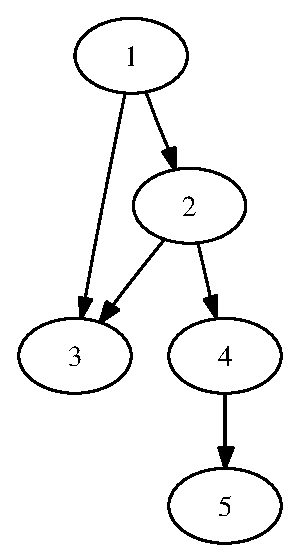
\epsfig{file=Figures/graph0,scale=0.6}

  \caption{A simple graph.}
  \label{fig:graph0}
\end{figure}



\noindent
The graph given by the relation \texttt{R} contains only the direct connections of vertices.  For example, in
the graph shown in Figure \ref{fig:graph0}, there is a direct connection from vertex $1$ to vertex $2$ and
another direct connection from vertex $2$ to vertex $4$.  Intuitively, vertex $4$ is reachable from vertex $1$,
since from vertex $1$ we can first reach vertex $2$ and from vertex $2$ we can then reach vertex $4$.  However,
there is is no direct connection between the vertices $1$ and $4$.  To make this more formal, define
a \colorbox{amethyst}{\blue{path}} 
of a graph $R$ as a list of vertices
\\[0.2cm]
\hspace*{1.3cm}
$[x_1, x_2, \cdots, x_n]$ \quad such that \quad $\pair(x_i,x_{i+1}) \in R$ \quad for all $i=1,\cdots,n-1$.
\\[0.2cm]
In this case, the path $[x_1, x_2, \cdots, x_n]$ is written as
\\[0.2cm]
\hspace*{1.3cm}
$x_1 \mapsto x_2 \mapsto \cdots \mapsto x_n$
\\[0.2cm]
and has the \blue{length} $n-1$.  It is important to note that the length of a path
$[x_1,x_2,\cdots,x_n]$ is defined as the number of edges connecting the vertices and not as the
number of vertices appearing in the path.

Furthermore,  two vertices $a$ and $b$ are said to be \colorbox{amethyst}{\blue{connected}} iff there exists a path
\\[0.2cm]
\hspace*{1.3cm}
$[x_1,\cdots,x_n]$ \quad such that \quad $a = x_1$ \quad and \quad $b = x_n$.
\\[0.2cm]
The goal of this section is to develop an algorithm that checks whether two vertices $a$ and $b$ are connected.
Furthermore, we want to be able to compute the corresponding path connecting the vertices $a$ and $b$.


\subsection{Computing the Transitive Closure of a Relation}
We have already noted that a graph can be represented as the set of its edges and hence as a \blue{relation}.
In order to decide whether there is a path connecting two vertices we have to compute the 
\href{https://en.wikipedia.org/wiki/Transitive_closure}{transitive closure} $R^+$ of a relation $R$.  
In the \href{https://github.com/karlstroetmann/Lineare-Algebra/blob/master/Script/lineare-algebra.pdf}{math lecture}
we have seen that the transitive closure $R^+$ can be computed as follows:
\\[0.2cm]
\hspace*{1.3cm}
$R^+ = \bigcup\limits_{n=1}^{\infty} R^n = R^1 \cup R^2 \cup R^3 \cup \cdots$  
\\[0.2cm]
Initially, this formula might look intimidating as it suggests an infinite computation.
Fortunately, it turns out that we do not have to compute all powers of the form $R^n$.  Let me
explain the reason that allows us to cut the computation short.  
\begin{enumerate}
\item $R$ is the set of direct connections between two vertices.
\item $R^2$ is the same as $R \circ R$ and this relational product is defined as
      \\[0.2cm]
      \hspace*{1.3cm}
       $R \circ R = \{ \pair(x,z) \mid \exists y \colon \pair(x,y) \in R \wedge \pair(y,z) \in R \}$.
      \\[0.2cm]
      Hence, $R \circ R$ contains those pairs $\pair(x,z)$ that are connected via one intermediate vertex $y$,
      i.e.~there is a path of the form $x \mapsto y \mapsto z$ that connects $x$ and $z$.  This path
      has length 2.  In general, we can show by induction that $R^n$ connect those pairs that are
      connected by a path of length $n$.  The induction step of this proof runs as follows:
\item $R^{n+1}$ is defined as $R \circ R^{n}$ and therefore we have
      \\[0.2cm]
      \hspace*{1.3cm}
      $R \circ R^n = \{ \pair(x,z) \mid \exists y \colon \pair(x,y) \in R \wedge \pair(y,z) \in R^n \}$.
      \\[0.2cm]
      As $\pair(y,z) \in R^n$, the induction hypothesis guarantees that the vertices $y$ and $z$ are
      connected by a path of length $n$.  Hence, this 
      path has the form
      \\[0.2cm]
      \hspace*{1.3cm}
      $\underbrace{y \mapsto \cdots \mapsto z}_{\mbox{\scriptsize path of length $n$.}}$
      \\[0.2cm]
      Adding $x$ at the front of this path will produce the path
      \\[0.2cm]
      \hspace*{1.3cm}
      $x \mapsto y \mapsto \cdots \mapsto z$.
      \\[0.2cm]
      This path has a length of $1 + n = n + 1$ and, furthermore, connects $x$ and $z$.  Hence $R^{n+1}$
      contains those pairs $\pair(x, z)$ that are connected by a path of length $n+1$.
\end{enumerate}
Now the important observation is the following. The set of all vertices is finite.  For the arguments sake, let
us assume there are $k$ vertices.  But then every path that has a length of  $k$ or greater must contain one
vertex that is visited at least twice and hence this path is longer than necessary, i.e.~there is a shorter path that
connects the same vertices.  Therefore, for a finite graph with $k$ vertices, the formula to compute the
transitive closure can be simplified as follows:
\\[0.2cm]
\hspace*{1.3cm} 
$\ds R^+ = \bigcup\limits_{i=1}^{k-1} R^i$.
\\[0.2cm]
While we could use this formula as its stands, it is more efficient to use a \blue{fixed-point iteration} instead.
To this end, we prove that the transitive closure $R^+$ satisfies the following equation:
\begin{equation}
  \label{fixpunkt}
  R^+ = R \cup R \circ R^+. 
\end{equation}
Let me remind you that the precedence of the operator $\circ$ 
is higher than the precedence of the operator $\cup$.  Therefore, the expression $R \cup R \circ R^+$ is parenthesized
as $R \cup (R \circ R^+)$.  Equation \ref{fixpunkt} can be proven algebraically.  We have:
\\[0.2cm]
\hspace*{1.3cm}
$
\begin{array}{cll}
    & R \cup R \circ R^+ \\[0.2cm]
  = & R \cup R \circ \bigcup\limits_{i=1}^{\infty} R^i \\[0.4cm]
  = & R \cup R \circ \bigl(R^1 \cup R^2 \cup R^3 \cup \cdots \bigr) \\[0.2cm]
  = & R \cup \bigl(R \circ R^1 \cup R \circ R^2 \cup R \circ R^3 \cup \cdots \bigr) \\[0.2cm]
  = & R \cup \bigl(R^2 \cup R^3 \cup  R^4 \cup \cdots \bigr)  \\[0.2cm]
  = & R^1 \cup \bigl(R^2 \cup R^3 \cup  R^4 \cup \cdots \bigr) \\[0.2cm]
  = & \bigcup\limits_{i=1}^{\infty} R^i \\[0.4cm]
  = & R^+.
\end{array}
$
\\[0.2cm]
Equation  \ref{fixpunkt} can now be used to compute $R^+$ via a fixed-point iteration.
To this end, let us define a sequence of relations $(T_n)_{n \in \mathbb{N}}$ by induction on $n$:
\begin{enumerate}
\item[I.A.] $n = 0$: 

            $T_0 = R$
\item[I.S.] $n \mapsto n+1$:

            $T_{n+1} = R \cup R \circ T_n$. 
\end{enumerate}
The relation  $T_n$ can be expressed via the relation $R$, we have
\begin{enumerate}
\item $T_0 = R$.
\item $T_1 = R \cup R \circ T_0 = R \cup R \circ R = R^1 \cup R^2$.
\item$\begin{array}[t]{lcl}
       T_2  & = & R \cup R \circ T_1 \\
            & = & R \cup R \circ (R^1 \cup R^2) \\
            & = & R^1 \cup R^2 \cup R^3. \\
       \end{array}
      $
\end{enumerate}
In general, we can show by induction that
\\[0.2cm]
\hspace*{1.3cm}
$T_n = \bigcup\limits_{i=1}^{n+1} R^i$
\\[0.2cm]
holds for all $n \in \mathbb{N}$.  The base case of this proof is immediate form the definition of $T_0$.
In the induction step we observe the following:
\\[0.2cm]
\hspace*{1.3cm}
$
 \begin{array}{lcll}
   T_{n+1} & = & \ds R \cup R \circ T_n & \mbox{(by definition)} \\[0.2cm]
           & = & \ds R \cup R \circ \biggl(\bigcup\limits_{i=1}^{n+1} R^i\biggr) &
                 \mbox{(by induction hypothesis)} \\[0.4cm]
           & = & \ds R \cup R \circ \left(R \cup \cdots \cup R^{n+1}\right) \\[0.2cm] 
           & = & \ds R \cup R^2 \cup \cdots \cup R^{n+2}  &
                 \mbox{(by the distributivity of $\circ$ over $\cup$)} \\[0.2cm]
           & = & \ds \bigcup\limits_{i=1}^{n+2} R^i & \Box 
   \end{array}
$
\\[0.2cm]
The sequence $(T_n)_{n\in\mathbb{N}}$ has another useful property:  It is 
\blue{monotonically increasing}.  In general, a sequence of sets $(X_n)_{n\in\mathbb{N}}$ is called
\blue{monotonically increasing} iff we have
\\[0.2cm]
\hspace*{1.3cm}
$\forall n \in \mathbb{N}: X_n \subseteq X_{n+1}$,
\\[0.2cm]
i.e.~the sets $X_n$ get bigger with growing index $n$.
The monotonicity of the sequence  $(T_n)_{n \in \mathbb{N}}$ is an immediate consequence of the equation
\\[0.2cm]
\hspace*{1.3cm}
$\ds T_n = \bigcup\limits_{i=1}^{n+1} R^i$ 
\\[0.2cm]
because we have:
\\[0.2cm]
\hspace*{1.3cm}
$
\begin{array}[t]{llcl}
                & \ds T_n \subseteq T_{n+1} \\[0.2cm]
\Leftrightarrow & \ds \bigcup\limits_{i=1}^{n+1} R^i \subseteq \bigcup\limits_{i=1}^{n+2} R^i \\[0.5cm]
\Leftrightarrow & \ds \bigcup\limits_{i=1}^{n+1} R^i \subseteq \bigcup\limits_{i=1}^{n+1} R^i \cup R^{n+2} \\
\end{array}
$
\\[0.2cm]
If the relation  $R$ is finite, then the transitive closure $R^+$ is finite, too.  The sets $T_n$ 
are all subsets of $R^+$ because we have
\\[0.2cm]
\hspace*{1.3cm}
$\ds T_n = \bigcup\limits_{i=1}^{n+1} R^i \subseteq \bigcup\limits_{i=1}^{\infty} R^i = R^+$ \quad for all $n \in \mathbb{N}$.
\\[0.2cm]
Hence the sets $T_n$ can not grow indefinitely.  Because of the monotonicity of the sequence 
$(T_n)_{n\in\mathbb{N}}$ it follows that there exists an index  $k \in \mathbb{N}$ such that the sets $T_n$ do
not grow any further once $n$ has reached $k$, i.e.~we have
\\[0.2cm]
\hspace*{1.3cm}
$\ds \forall n \in \mathbb{N}:( n \geq k \rightarrow T_n = T_k)$.
\\[0.2cm]
But this implies that
\\[0.2cm]
\hspace*{1.3cm}
$\ds T_n = \bigcup\limits_{i=1}^{n+1} R^i = \bigcup\limits_{i=1}^{\infty} R^i = R^+$ 
\quad holds for all $n \geq k$.
\\[0.2cm]
Therefore, the algorithm for computing  $R^+$ iterates the equation 
\\[0.2cm]
\hspace*{1.3cm}
$\ds T_{n+1} = R \cup R \circ T_n$
\\[0.2cm]
until the equation  $T_{n+1} = T_n$ is satisfied, since this implies that $T_n = R^+$.


\begin{figure}[!ht]
  \centering
\begin{Verbatim}[ frame         = lines, 
                  framesep      = 0.3cm, 
                  labelposition = bottomline,
                  numbers       = left,
                  numbersep     = -0.2cm,
                  xleftmargin   = 0.8cm,
                  xrightmargin  = 0.8cm,
                ]
    transClosure = procedure(R) {
        T = R;
        while (true) {
            oldT = T;
            T    = R + product(R, T);
            if (T == oldT) {
                return T;
            }
        }
    };
    product = procedure(R1, R2) {
        return { [x,z] : [x,y] in R1, [y,z] in R2 };
    };
    R = { [1,2], [2,3], [1,3], [2,4], [4,5] };
    print( "R = ", R );
    print( "Computing the transitive closure of R:" );
    T = transClosure(R);
    print( "R+ = ", T );
\end{Verbatim} 
\vspace*{-0.3cm}
\caption{Computing the transitive closure.}  
\label{fig:transitive-closure.py}
\end{figure} %\$

\noindent
The program 
\href{https://github.com/karlstroetmann/Logik/blob/master/Python/transitive-closure.py}{\texttt{transitive-closure.py}}
that is shown in Figure
\ref{fig:transitive-closure.py} on page \pageref{fig:transitive-closure.py} shows an implementation of this idea.
The program produces the following output:
\begin{verbatim}
    R = {[1, 2], [2, 3], [1, 3], [2, 4], [4, 5]}
    Computing the transitive closure of R:
    R+ = {[1, 2], [1, 3], [1, 4], [1, 5], [2, 3], [2, 4], [2, 5], [4, 5]}
\end{verbatim}
The transitive closure $R^+$ of a relation $R$ has a very intuitive interpretation:
$R^+$:  It contains all pairs $\pair(x,y)$ such that there is a path leading from 
$x$ to $y$.  
The function $\texttt{product}(R_1, R_2)$ computes the relational product $R_1\circ R_2$ 
according to the formula
\\[0.2cm]
\hspace*{1.3cm}
$R_1 \circ R_2 = \{ \langle x, z \rangle \mid \exists y: \pair(x,y) \in R_1 \wedge \pair(y,z) \in R_2 \}$.
\\[0.2cm]
The implementation of the procedure \texttt{product} shows the most general way to define a set in
\textsl{Python}.  In general, a set can be defined via an expression of the form
\\[0.2cm]
\hspace*{1.3cm}
$\{\; \textsl{expr} \;\texttt{:}\; [x^{(1)}_1, \cdots, x^{(1)}_{n(1)}] \;\texttt{in}\; s_1,
     \cdots, [x^{(k)}_1, \cdots, x^{(k)}_{n(k)}] \;\texttt{in}\; s_k \;\texttt{|}\;
     \textsl{cond} \;\}
$.
\\[0.2cm]
Here, for all $i=1, \cdots, k$ the variable $s_i$ denotes a set of lists of length $n(i)$.  When the
expression given above is evaluated, the variables $x^{(i)}_1, \cdots, x^{(i)}_{n(i)}$ are replaced
by the corresponding values in the lists from the sets  $s_i$.  For example, if we define
\begin{verbatim}
    s1 = { [ 1, 2, 3 ], [ 5, 6, 7 ] };
    s2 = { [ "a", "b" ], [ "c", "d" ] };
    m = { [ x1, x2, x3, y1, y2 ] : [ x1, x2, x3 ] in s1, [ y1, y2 ] in s2 };
\end{verbatim}
then the set  \texttt{m} has the following value:
\begin{verbatim}
    { [1, 2, 3, "a", "b"], [5, 6, 7, "c", "d"],  
      [1, 2, 3, "c", "d"], [5, 6, 7, "a", "b"] }
\end{verbatim}


\subsection{Computing the Paths}
So far, given a graph represented by a relation $R$ and two vertices $x$ and $y$, we can only check
whether there is a path leading from $x$ to $y$, but we cannot compute this path.  In this
subsection we will extend the procedure \texttt{transClosure} so that it will also compute the
corresponding path.  The main idea is to extend the notion of a relational product to the notion of
a \blue{path product}, where a \blue{path product} is defined on sets of paths.  In order to do so,
we introduce three functions for lists.
\begin{enumerate}
\item Given a list $p$, the function $\texttt{first}(p)$ returns the first element of $p$: 
      \\[0.2cm]
      \hspace*{1.3cm}
      $\texttt{first}\bigl([x_1,\cdots,x_m]\bigr) = x_1$.
\item Given a list $p$, the function $\texttt{last}(p)$ returns the last element of $p$: 
      \\[0.2cm]
      \hspace*{1.3cm}
      $\texttt{last}\bigl([x_1,\cdots,x_m]\bigl) = x_m$.
\item If $p = [ x_1, \cdots, x_m ]$ and $q =[ y_1, \cdots, y_n ]$ are two path such that
      $\texttt{first}(q) = \texttt{last}(p)$, we define the \blue{join} of $p$ and $q$ as \\[0.2cm]
      \hspace*{1.3cm}
      $p \oplus q = [x_1, \cdots, x_m, y_2, \cdots, y_n ]$.
\end{enumerate}
If $P_1$ and $P_2$ are sets of paths, we define the  \blue{path product} of
$P_1$ and $P_2$ as follows: \\[0.2cm]
\hspace*{1.3cm} 
$P_1 \bullet P_2 = 
\bigl\{\; p_1 \oplus p_2 \mid p_1 \in P_1 \wedge p_2 \in P_2 \wedge \texttt{last}(p_1) =
\texttt{first}(p_2) \;\bigr\}
$.

\begin{figure}[!ht]
  \centering
\begin{Verbatim}[ frame         = lines, 
                  framesep      = 0.3cm, 
                  labelposition = bottomline,
                  numbers       = left,
                  numbersep     = -0.2cm,
                  xleftmargin   = 0.8cm,
                  xrightmargin  = 0.8cm,
                ]
    transClosure = procedure(R) {
        P = R;
        while (true) {
            oldP = P;
            P    = R + pathProduct(R, P);
            print(P);
            if (P == oldP) {
                return P;
            }
        }
    };
    pathProduct = procedure(P, Q) {
        return { join(x, y) : x in P, y in Q | x[-1] == y[1] };
    };    
    join = procedure(p, q) {
        return p + q[2..];
    };
    R = { [1,2], [2,3], [1,3], [2,4], [4,5] };
    print( "R = ", R );
    print( "computing all paths" );
    P = transClosure(R);
    print( "P = ", P );
\end{Verbatim} 
\vspace*{-0.3cm}
\caption{Computing all connections.}  \label{fig:path.py}
\end{figure} %\$

\begin{figure}[!ht]
  \centering
  \vspace*{-9cm}

  \epsfig{file=Figures/graph-zykl,scale=0.5}
  \vspace*{-1cm}

  \caption{A graph with a cycle.}
  \label{fig:graph-zykl}
\end{figure}

Using the notion of a \blue{path product} we are able to extend the program shown in Figure
\ref{fig:transitive-closure.py} such that it computes all paths between two vertices.
The resulting program
\href{https://github.com/karlstroetmann/Logik/blob/master/Python/path.py}{\texttt{path.py}}
is shown in Figure \ref{fig:path.py} on page \pageref{fig:path.py}.
Unfortunately, the program does not work any more if the graph is \blue{cyclic}.  A graph is defined
to be \blue{cyclic} if there is a path of length greater than $1$ that starts and ends at the same
vertex.  This path is then called a \blue{cycle}.
Figure \ref{fig:graph-zykl} on page \pageref{fig:graph-zykl} shows a cyclic graph.  This graph is
cyclic because it contains the path
\\[0.2cm]
\hspace*{1.3cm}
\texttt{[1, 2, 4, 1]}
\\[0.2cm]
and this path is a cycle.
The problem with this graph is that it contains an infinite number of paths that connect the vertex
1 with the vertex 2: \\[0.2cm]
\hspace*{1.3cm}
$[ 1, 2 ]$, $[ 1, 2, 4, 1, 2 ]$, 
$[ 1, 2, 4, 1, 2, 4, 1, 2 ]$, 
$[ 1, 2, 4, 1, 2, 4, 1, 2, 4, 1, 4 ]$, $\cdots$
\\[0.2cm]
Of course, there is no point in computing a path that visits a vertex more than once as these paths
contain cycles.  Our goal is to eliminate all those paths that contain cycles.


\begin{figure}[!ht]
  \centering
\begin{Verbatim}[ numbers       = left,
                  numbersep     = -0.2cm,
                  frame         = lines, 
                  framesep      = 0.3cm, 
                  labelposition = bottomline,
                  xleftmargin   = 0.0cm,
                  xrightmargin  = 0.0cm,
                ]
    pathProduct = procedure(P, Q) {
        return { join(x,y) : x in P, y in Q | x[-1] == y[1] && noCycle(x, y) };
    };
    noCycle = procedure(L1, L2) {
        return #({ x : x in L1 } * { x : x in L2 }) == 1;
    };
\end{Verbatim} 
\vspace*{-0.3cm}
\caption{Computing the connections in a cyclic graph.}  
\label{fig:path-cyclic.py}
\end{figure} %\$

Figure \ref{fig:path-cyclic.py} on page shows how the implementation of the function
\texttt{pathProduct} has to be changed so that the resulting program
\href{https://github.com/karlstroetmann/Logik/blob/master/Python/path-cyclic.py}{\texttt{path-cyclic.py}}
works also for cyclic graphs. 
\begin{enumerate}
\item In line 2, we compute only those paths that are not cyclic.
\item Line 5 tests, whether the join  $\texttt{L1} \oplus \texttt{L2}$ is cyclic.  The join
      of \texttt{L1} and \texttt{L2} is cyclic iff the lists \texttt{L1} and \texttt{L2} have more
      than one common element. 
      The lists \texttt{L1} and \texttt{L2} will always have at least one common element, as we join
      these lists only if the last element of \texttt{L1} is equal to the first element of  \texttt{L2}.
      If there would be an another vertex common to \texttt{L1} and \texttt{L2}, then the path
      $\texttt{L1} \oplus \texttt{L2}$ would be cyclic.
\end{enumerate}

In general, we are not really interested to compute all possible paths between two given vertices
\texttt{x} and \texttt{y}.  Instead, we just want to compute the shortest path leading from \texttt{x} to \texttt{y}.
Figure \ref{fig:find-path.py} on page \pageref{fig:find-path.py} shows the procedure \texttt{reachable}. 
This procedure takes three arguments:
\begin{enumerate}
\item \texttt{x} and \texttt{y} are vertices of a graph.
\item \texttt{R} is a binary relation representing a directed graph.
\end{enumerate}
The call  \texttt{reachable(x, y, R)} checks whether \texttt{x} and \texttt{y} are connected and, furthermore,
computes the shortest path from \texttt{x} to \texttt{y}, provided such a path exists.
The complete program can be found in the file
\href{https://github.com/karlstroetmann/Logik/blob/master/Python/find-path.py}{\texttt{find-path.py}}.
Next, we discuss the implementation of the procedure  \texttt{reachable}.
\begin{enumerate}
\item Line 2 initializes the set \texttt{P}.  After $n$ iterations, this set will contain all paths
      that start in the vertex \texttt{x} and that have a length of at most $n$.

      Initially, there is just the trivial path \texttt{[x]} that starts in \texttt{x} and has
      length $0$.
\item Line 5 tries to extend all previously computed paths by one step.
      If we are lucky, the set \texttt{P} is increased in this step.
\item Line 6 selects all those paths from the set \texttt{P} that lead to the vertex \texttt{y}.
      These paths are stored in the set \texttt{Found}.
\item Line 7 checks whether we have indeed found a path ending at \texttt{y}.  This is the case if
      the set \texttt{Found} is not empty.  
      In this case, we return any of these paths.
\item If we have not yet found the vertex \texttt{y} and, furthermore, we have not been able to find
      any new paths during this iteration,  the procedure returns in line 11.
      As the \texttt{return} statement in line 11 does not return a value, the procedure will
      instead return the undefined value $\Omega$.
\end{enumerate}
The procedure call \texttt{reachable(x,y R)} will compute the \textbf{shortest} path connecting
\texttt{x} and \texttt{y} because it computes path with increasing length.  The first iteration
computes all paths starting in \texttt{x} that have a length of at most 1, the second iteration
computes all paths starting in \texttt{x} that have a length of at most 2, and in general the $n$-th
iteration computes all paths starting in \texttt{x} that have a length of at most $n$.  Hence, if
there is a path of length $n$, then this path will be found in the $n$-iteration unless a shorter path has
already been found in a previous iteration.  

\remarkEng
The algorithm described above is known as 
\href{https://en.wikipedia.org/wiki/Breadth-first_search}{breadth first search}. \eox 



\begin{figure}[!ht]
  \centering
\begin{Verbatim}[ frame         = lines, 
                  framesep      = 0.3cm, 
                  labelposition = bottomline,
                  numbers       = left,
                  numbersep     = -0.2cm,
                  xleftmargin   = 0.8cm,
                  xrightmargin  = 0.8cm,
                ]
    reachable = procedure(x, y, R) {
        P = { [x] };
        while (true) {
            oldP  = P;
            P     = P + pathProduct(P, R);
            Found = { l : l in P | l[-1] == y };
            if (Found != {}) {
                return arb(Found);
            }
            if (P == oldP) {
                return;
            }
        }
    };
\end{Verbatim} 
\vspace*{-0.3cm}
\caption{Finding the shortest path between two vertices.}  
\label{fig:find-path.py}
\end{figure}

\subsection{The Wolf, the Goat, and the Cabbage}
Next, we present an application of the theory developed so far.  We solve a problem from that has puzzled
the greatest agricultural economists for centuries.  The puzzle we want to solve is known as the 
\href{http://jeux.lulu.pagesperso-orange.fr/html/anglais/loupChe/loupChe1.htm}{wolf-goat-cabbage puzzle}:  
\vspace*{0.3cm}

\begin{minipage}[c]{14cm}
{\sl
An agricultural economist has to sell a wolf, a goat, and a cabbage on a market place.  In order to
reach the market place, she has to cross a river.  The boat that she can use is so small that it can
only accommodate either the goat, the wolf, or the cabbage in addition to the agricultural economist.
Now if the agricultural economist leaves the wolf alone with the goat, the wolf will eat the goat.
If, instead, the agricultural economist leaves the goat with the cabbage, the goat will eat the cabbage.
Is it possible for the agricultural economist to develop a schedule that allows her to cross the river
without either the goat or the cabbage being eaten?
}
\end{minipage}
\vspace*{0.3cm}

\noindent
In order to compute a schedule, we first have to model the problem.  The various \blue{states} of the problem will
be regarded as \blue{vertices} of a graph and this graph will be represented as a binary relation.
To this end we define the set
\\[0.2cm]
\hspace*{1.3cm} 
$\texttt{All} = \{ \squote{farmer}, \squote{wolf}, \squote{goat},\squote{cabbage} \}$.
\\[0.2cm]
Every node will be represented as a subset \texttt{S} of the set \texttt{All}.  The idea is that the set \texttt{S}
specifies those objects that are on the left side of the river.  We assume that initially the farmer
is on the left side of the river. 
Therefore, the set of all possible states can be defined as the set
\begin{verbatim}
        P = { S : S in 2 ** All | !problem(S) && !problem(All - S) };
\end{verbatim}
Here, we have used the procedure \texttt{problem} to check whether a given set \texttt{S} has a problem. 
Note that since \texttt{S} is the set of objects on the left side, the expression $\texttt{All - S}$
computes the set of objects on the right side of the river.

Next, a set \texttt{S} of objects has a problem if both of the following conditions
are satisfied:
\begin{enumerate}
\item The farmer is not an element of \texttt{S} and
\item either \texttt{S} contains both the goat and the cabbage or \texttt{S} contains both the wolf and the goat.
\end{enumerate}
Therefore, we can implement the function \texttt{problem} as follows:

\begin{verbatim}
    problem = procedure(S) {
        return !("farmer" in S)                                     && 
               ({"goat", "cabbage"} <= S || {"wolf", "goat"} <= S);
    };
\end{verbatim}
We proceed to compute the relation \texttt{R} that contains all possible transitions between
different states.  We will compute \texttt{R} using the formula:
\\[0.2cm]
\hspace*{0.75cm}
\texttt{R = R1 + R2;}
\\[0.2cm]
Here \texttt{R1} describes the transitions that result from the farmer crossing the river from left
to right, while \texttt{R2} describes the transitions that result from the farmer crossing the river
from right to left.  We can define the relation \texttt{R1} as follows:
\begin{verbatim}
    R1  = { [S, S - B]: S in P, B in 2 ** S
                       | S - B in P && "farmer" in B && #B <= 2
           };
\end{verbatim}
Let us explain this definition in detail:
\begin{enumerate}
\item Initially, \texttt{S} is the set of objects on the left side of the river.  Hence, \texttt{S}
      is an element of the set of all states that we have defined as \texttt{P}.
\item \texttt{B} is the set of objects that are put into the boat and that do cross the river.  Of
      course, for an object to go into the boat is has to be on the left side of the river to begin
      with.  Therefore, \texttt{B} is a subset of \texttt{S} and hence an element of the power set
      of \texttt{S}. 
\item Then  \texttt{S-B} is the set of objects that are left on the left side of the river after
      the boat has crossed.  Of course, the new state \texttt{S-B} has to be a state that does not
      have a problem.  Therefore, we check that \texttt{S-B} is an element of \texttt{P}.
\item Furthermore, the farmer has to be in the boat.  This explains the condition 
      \\[0.2cm]
      \hspace*{1.3cm}
      \texttt{\symbol{39}farmer\symbol{39} in B}.
\item Finally, the boat can only have two passengers.  Therefore, we have added the condition
      \\[0.2cm]
      \hspace*{1.3cm}
      \texttt{\#B <= 2}.
\end{enumerate}
Next, we have to define the relation \texttt{R2}.  However, as crossing the river from right to left
is just the reverse of crossing the river from left to right, \texttt{R2} is just the inverse of
\texttt{R1}.   Hence we define:
\\[0.2cm]
\hspace*{1.3cm}
\texttt{R2  = \{ [y, x] : [x, y] in R1 \};}
\\[0.2cm]
Finally, the start state has all objects on the left side.  Therefore, we have
\\[0.2cm]
\hspace*{1.3cm}
\texttt{start = All;}
\\[0.2cm]
In the end, all objects have to be on the right side of the river.  That means that nothing is left
on the left side.  Therefore, we define
\\[0.2cm]
\hspace*{1.3cm}
\texttt{goal = \{\};}
\\[0.2cm]
Figure \ref{fig:wolf-ziege} on page \pageref{fig:wolf-ziege} shows the program
\href{https://github.com/karlstroetmann/Logik/blob/master/Python/wolf-goat-cabbage.py}{\texttt{wolf-goat-cabbage.py}}
that combines the statements shown so far.  The solution computed by this program is shown in Figure
 \ref{fig:wolf-ziege-solution}.

\begin{figure}[!ht]
  \centering
\begin{Verbatim}[ codes         = {\catcode`$=3\catcode`_=8\catcode`^=7},
                  frame         = lines, 
                  framesep      = 0.3cm, 
                  labelposition = bottomline,
                  numbers       = left,
                  numbersep     = -0.2cm,
                  xleftmargin   = 0.8cm,
                  xrightmargin  = 0.8cm,
                ]
    problem = procedure(S) {
        return !("farmer" in S)                                     && 
               ({"goat", "cabbage"} <= S || {"wolf", "goat"} <= S);
    };
    
    All = { "farmer", "wolf", "goat", "cabbage" };
    P   = { S : S in 2 ** All | !problem(S) && !problem(All - S) };
    R1  = { [S, S - B]: S in P, B in 2 ** S
                       | S - B in P && "farmer" in B && #B <= 2
           };
    R2  = { [y, x] : [x, y] in R1 };
    R   = R1 + R2;
    
    start = All;
    goal  = {};
    
    path  = reachable(start, goal, R);
\end{Verbatim} 
\vspace*{-0.3cm}
\caption{Solving the wolf-goat-cabbage problem.}  
\label{fig:wolf-ziege}
\end{figure}


\begin{figure}[!ht]
  \centering
\begin{Verbatim}[ codes         = {\catcode`$=3\catcode`_=8\catcode`^=7},
                  frame         = lines, 
                  framesep      = 0.3cm, 
                  labelposition = bottomline,
                  numbers       = left,
                  numbersep     = -0.2cm,
                  xleftmargin   = 0.8cm,
                  xrightmargin  = 0.8cm,
                ]
    {"cabbage", "farmer", "goat", "wolf"}                                 {}
                             >>>> {"farmer", "goat"} >>>> 
    {"cabbage", "wolf"}                                   {"farmer", "goat"}
                             <<<< {"farmer"} <<<< 
    {"cabbage", "farmer", "wolf"}                                   {"goat"}
                             >>>> {"farmer", "wolf"} >>>> 
    {"cabbage"}                                   {"farmer", "goat", "wolf"}
                             <<<< {"farmer", "goat"} <<<< 
    {"cabbage", "farmer", "goat"}                                   {"wolf"}
                             >>>> {"cabbage", "farmer"} >>>> 
    {"goat"}                                   {"cabbage", "farmer", "wolf"}
                             <<<< {"farmer"} <<<< 
    {"farmer", "goat"}                                   {"cabbage", "wolf"}
                             >>>> {"farmer", "goat"} >>>> 
    {}                                 {"cabbage", "farmer", "goat", "wolf"}
\end{Verbatim} 
\vspace*{-0.3cm}
\caption{A schedule for the agricultural economist.}  
\label{fig:wolf-ziege-solution}
\end{figure}


\section{Terms and Matching}
So far we have seen the basic data structures of \setlx\ like numbers, string, sets, and lists.
There is one more data structure that is supported by \setlx.  This is the data structure of
\colorbox{amethyst}{\blue{terms}}.  
This data structure is especially useful when we develop programs that deal with mathematical formulas.
For example, in this section we will develop a program that reads a string like 
\\[0.2cm]
\hspace*{1.3cm}
``\texttt{x * exp(x)}'',
\\[0.2cm]
interprets this string as describing the real valued function 
\\[0.2cm]
\hspace*{1.3cm}
$x \mapsto x \cdot \exp(x)$, 
\\[0.2cm]
and then takes the derivative of this function with respect to the variable $x$.  This program is
easy to implement if real valued functions are represented as terms.  The reason is that \setlx\ provides 
\colorbox{amethyst}{\blue{matching}} for terms.  We will define this notion later.  Matching
is one of the main ingredients of the programming language \href{https://en.wikipedia.org/wiki/Prolog}{Prolog}.
This programming language was quite popular in artificial intelligence during the eighties and has
inspired the matching that is available in \textsl{Python}.


\subsection{Constructing and Manipulating Terms}
In order to build terms, we first need \colorbox{amethyst}{\blue{functors}}.  It is important not to confuse functors with
function symbols.  Therefore, functors have to be preceded by the character  
``\texttt{@}''.
For example, the following strings can be used as functors:
\\[0.2cm]
\hspace*{1.3cm}
\texttt{@f}, \quad \texttt{@FabcXYZ}, \quad \texttt{@sum}, \quad \texttt{@Hugo\_}.
\\[0.2cm]
However, in the expression ``\texttt{@f}'', the string ``\texttt{f}'' is the functor.  The
character ``\texttt{@}'' is only used as an escape character that tells us that ``\texttt{f}'' is
not a function symbol but rather a functor.  Next, we define \colorbox{amethyst}{\blue{terms}}.  If $F$ is a functor and 
$t_1$, $t_2$, $\cdots$, are any values, i.e.~they could be number, strings, lists, sets, or terms
themselves, then
\\[0.2cm]
\hspace*{1.3cm}
$\texttt{@}F(t_1, t_2, \cdots, t_n)$
\\[0.2cm]
is a term.  Syntactically, terms look very similar to function calls.  The only difference between a function call
and a term is the following: 
\begin{enumerate}
\item A function call starts with a function symbol. 
\item A term starts with a functor. 
\end{enumerate}


\examplesEng
\begin{enumerate}
\item \texttt{@Address(\symbol{39}Coblitzallee 1-9\symbol{39}, 68163, \symbol{39}Mannheim\symbol{39})}

      is a term that represents an address.
\item \texttt{@product(@variable(\symbol{39}x\symbol{39}), @exp(@variable(\symbol{39}x\symbol{39})))}

      is a term that represents the  function $x \mapsto x \cdot \exp(x)$.  
      \eox
\end{enumerate}
At this point you might ask how terms are evaluated.  The answer is that terms
\colorbox{amethyst}{are not evaluated!}  
Terms are used to represent data in a way that is both concise and readable.  Hence, terms are values like
numbers, sets or strings.  As terms are values, they don't need to be evaluated.

Let us demonstrate a very simple application of terms.  Imagine that \setlx\ wouldn't provide lists as a native data
type.  Then, we could implement lists via terms.  First, we would use a functor to represent the empty list.
Let us choose the functor \texttt{nil} for this purpose.  Hence, we have
\\[0.2cm]
\hspace*{1.3cm}
$\texttt{@nil()} \;\widehat{=}\; \texttt{[]}$,
\\[0.2cm]
where we read the symbol ``$\widehat{=}$'' as ``corresponds to''.
Note that the parentheses after the functor  \texttt{nil} are \colorbox{amethyst}{necessary!}  Next, in order to represent
a list with first element $x$ and a list $r$ of remaining elements we use the functor \texttt{cons}.
Then we have the correspondence
\\[0.2cm]
\hspace*{1.3cm}
$\texttt{@cons}(x, r) \;\widehat{=}\; \texttt{[}x\texttt{]} + r$. 
\\[0.2cm]
Concretely, the list \texttt{[1,2,3]} is represented as the term
\\[0.2cm]
\hspace*{1.3cm}
\texttt{@cons(1, @cons(2, @cons(3, @nil())))}.
\\[0.2cm]
The programming language \textsl{Prolog} represents lists internally in a similar form.

\setlx\ provides two functions that allow us to extract the components of a term.  Furthermore, there is a
function for constructing terms.  These functions are described next.
\begin{enumerate}
\item The function \texttt{fct} returns the functor of a given term.
      If  $t$ is a term of the form $\at F(s_1,\cdots,s_n)$, then the result returned by the expression
      \\[0.2cm]
      \hspace*{1.3cm}
      $\texttt{fct}(\at F(s_1,\cdots,s_n))$
      \\[0.2cm]
      is the functor $F$ of this term.  For example the expression
      \\[0.2cm]
      \hspace*{1.3cm}
      \texttt{fct(@cons(1, @cons(2, @cons(3, @nil()))))}
      \\[0.2cm]
      returns the string  \texttt{\symbol{39}cons\symbol{39}} as its result.
\item The function \texttt{args} returns the arguments of a term.
      If  $t$ is a term of the form $\at F(s_1,\cdots,s_n)$, then
      \\[0.2cm]
      \hspace*{1.3cm}
      $\mathtt{args}(\at F(s_1,\cdots,s_n))$
      \\[0.2cm]
      returns the list $[s_1, \cdots, s_n]$. For example, the expression
      \\[0.2cm]
      \hspace*{1.3cm}
      \texttt{args(\at cons(1, \at cons(2, \at cons(3, \at nil()))))}
      \\[0.2cm]
      is evaluated as
      \\[0.2cm]
      \hspace*{1.3cm}
      \texttt{[1, \at cons(2, \at cons(3, \at nil()))]}.
\item If $f$ is the name of a functor and  $l$ is a list, then the function \texttt{makeTerm} can be invoked as
      \\[0.2cm]
      \hspace*{1.3cm}
      $t \;\mathtt{=}\; \texttt{makeTerm}(f,l)$.
      \\[0.2cm]
      This expression generates a term $t$ such that $f$ is the functor and $l$ is the list of its
      arguments.  Therefore we have
      \\[0.2cm]
      \hspace*{1.3cm}
      $\mathtt{fct}(t) = f$  \quad und \quad $\mathtt{args}(t) = l$.
      \\[0.2cm]
      For example, the expression
      \\[0.2cm]
      \hspace*{1.3cm}
      \texttt{makeTerm(\symbol{39}cons\symbol{39}, [ 1, \at nil() ])}
      \\[0.2cm]
      returns the result
      \\[0.2cm]
      \hspace*{1.3cm}
      \texttt{\at cons(1, \at nil())}.
\end{enumerate}

\begin{figure}[!ht]
\centering
\begin{Verbatim}[ frame         = lines, 
                  framesep      = 0.3cm, 
                  firstnumber   = 1,
                  labelposition = bottomline,
                  numbers       = left,
                  numbersep     = -0.2cm,
                  xleftmargin   = 0.8cm,
                  xrightmargin  = 0.8cm,
                ]
    append = procedure(l, x) {
        if (fct(l) == "nil") {
            return @cons(x, @nil());  
        }
        [head, tail] = args(l);
        return @cons(head, append(tail, x));
    };
    l = @cons(1, @cons(2, @cons(3, @nil()))); // corresponds to [1,2,3]
    print(append(l, 4));
\end{Verbatim}
\vspace*{-0.3cm}
\caption{Appending an element at the end of a list.}
\label{fig:append.py}
\end{figure}

Figure \ref{fig:append.py} on page \pageref{fig:append.py} shows the
program \href{https://github.com/karlstroetmann/Logik/blob/master/Python/append.py}{\texttt{append.py}}.
This program implements the function \texttt{append}.  As its first arguments, this function takes a list \texttt{l}
that is represented as a term.  As its second argument,  it takes an object \texttt{x}.  The purpose of the expression
\\[0.2cm]
\hspace*{1.3cm}
$\texttt{append}(\texttt{l}, \texttt{x})$
\\[0.2cm]
is to append the object \texttt{x} at the end of the list \texttt{l}.  The implementation of the function \texttt{append}
assumes that the list \texttt{l} is represented as a term using the functors ``\texttt{cons}'' and ``\texttt{nil}''.
\begin{enumerate}
\item Line 2 checks whether the list  \texttt{l} is empty. The list \texttt{l} is empty iff we have
      $\texttt{l} = \texttt{\at nil()}$.  In the program we merely check the functor of the term \texttt{l}.  If the name of this functor is
      \texttt{\symbol{39}nil\symbol{39}}, then \texttt{l} is the empty list.
\item If \texttt{l} is not empty, then it must be a term of the form
      \\[0.2cm]
      \hspace*{1.3cm}
      $\texttt{l} = \texttt{\at cons(\textsl{head}, \textsl{tail})}$.
      \\[0.2cm]     
      Then, conceptually \texttt{head} is the first element of the list \texttt{l} and \texttt{tail} is the list of
      the remaining elements.  In this case, we need to recursively append \texttt{t} at the end of the list \texttt{tail}.
      Finally, the first element of the list \texttt{l}, which is called \texttt{head} in line 5, needs
      to be prepended to the list that is returned from the recursive invocation of \texttt{append}.
      This is done in line 6 by constructing the term 
      \\[0.2cm]
      \hspace*{1.3cm}
      \texttt{@cons(head, append(tail, x))}.
\end{enumerate}

\subsection{Matching}
It would be quite tedious if the functions \texttt{fct} and \texttt{args} were the only means to extract the
components of a term.  Figure \ref{fig:append-match.py} on page \pageref{fig:append-match.py}
shows the program
\href{https://github.com/karlstroetmann/Logik/blob/master/Python/append-match.py}{\texttt{append-match.py}}, 
that uses \blue{matching} to implement the function \texttt{append}.  
Line 3 checks, whether the list  \texttt{l} is empty, i.e.~whether \texttt{l} is identical to the term 
\texttt{@nil()}.  Line 4 is more interesting, as it combines two actions.
\begin{enumerate}
\item It checks, whether the list \texttt{l} is a term that starts with the functor \texttt{cons}.
\item If \texttt{l} does indeed starts with the functor \texttt{cons}, the arguments of this functor are
      extracted and assigned to the variables \texttt{head} and \texttt{tail}.
\end{enumerate}
Hence, if the \texttt{match} statement in line 4 is successful, the equation
\\[0.2cm]
\hspace*{1.3cm}
$\texttt{l} = \texttt{@cons(head, tail)}$
\\[0.2cm]
holds afterwards.


\begin{figure}[!ht]
\centering
\begin{Verbatim}[ frame         = lines, 
                  framesep      = 0.3cm, 
                  firstnumber   = 1,
                  labelposition = bottomline,
                  numbers       = left,
                  numbersep     = -0.2cm,
                  xleftmargin   = 0.8cm,
                  xrightmargin  = 0.8cm,
                ]
    append = procedure(l, x) {
        match (l) {
            case @nil():            return @cons(x, @nil());
            case @cons(head, tail): return @cons(head, append(tail, x));
        }
    };
\end{Verbatim}
\vspace*{-0.3cm}
\caption{Implementing \texttt{append} using a \texttt{match} statement.}
\label{fig:append-match.py}
\end{figure}
In general, a \texttt{match} statement has the structure that is shown in Figure \ref{fig:match}.
Here, $e$ is any expression that yields a term when evaluated.  The expressions 
$t_1$, $\cdots$, $t_n$ are so called \blue{patterns} that contain variables.  When the \texttt{match} statement
is executed, \textsl{Python} tries to bind the variables occurring in the pattern $t_1$ such that the resulting
expression is equal to $e$.  If this succeeds, the statements in  $\textsl{body}_1$ are executed and the
execution of the \texttt{match} statement ends.
Otherwise, the patterns $t_2$, $\cdots$, $t_n$ are tried one by one.  If the pattern $t_i$ is successfully
matched to $e$, the statements in $\textsl{body}_i$ are executed and the execution of the \texttt{match}
statement end.  If none of the patterns $t_1$, $\cdots$, $t_n$ can be matched with $e$, the statements in
$\textsl{body}_{n+1}$ are executed.


\begin{figure}[!ht]
  \centering
\begin{Verbatim}[ codes         = {\catcode`_=8\catcode`^=7},
                  frame         = lines, 
                  framesep      = 0.3cm, 
                  labelposition = bottomline,
                  numbers       = left,
                  numbersep     = -0.2cm,
                  commandchars  = \\\{\},
                  xleftmargin   = 0.8cm,
                  xrightmargin  = 0.8cm
                ]
      \texttt{\underline{match} (\(e\)) \{}
          \texttt{\underline{case}} \(t_1\) : \textsl{body}\(_1\) 
          \vdots
          \texttt{\underline{case}} \(t_n\) : \textsl{body}\(_n\)
          \texttt{\underline{default}:} \textsl{body}\(_{n+1}\)
      \texttt{\}}
\end{Verbatim}
\vspace*{-0.3cm}
\caption{Struktur eines \texttt{Match}-Blocks}  \label{fig:match}
\end{figure} 


\begin{figure}[!ht]
\centering
\begin{Verbatim}[ frame         = lines, 
                  framesep      = 0.3cm, 
                  firstnumber   = 1,
                  labelposition = bottomline,
                  numbers       = left,
                  numbersep     = -0.2cm,
                  xleftmargin   = 0.8cm,
                  xrightmargin  = 0.8cm,
                ]
    loadLibrary("termUtilities");  

    diff = procedure(t, x) {
        match (t) {
            case a + b :
                return diff(a, x) + diff(b, x);
            case a - b :
                return diff(a, x) - diff(b, x);
            case a * b :
                return diff(a, x) * b + a * diff(b, x);
            case a / b :
                return ( diff(a, x) * b - a * diff(b, x) ) / b * b;
            case a ** b :
                return diff( @exp(b * @ln(a)), x);
            case @ln(a) :
                return diff(a, x) / a;
            case @exp(a) :
                return diff(a, x) * @exp(a);
            case v | v == x :
                return 1;
            case y | isVariable(y) :  // must be different from x
                return 0;
            case n | isNumber(n):   
                return 0;  
         }
    };
    test = procedure(s) {
        t = parseTerm(s);
        v = parseTerm("x");
        d = diff(t, v);
        print("d/dx($s$) = $d$\n");
    };
    test("x ** x");
\end{Verbatim}
\vspace*{-0.3cm}
\caption{A function to perform symbolic differentiation.}
\label{fig:diff.py}
\end{figure}

\noindent
We close this section by showing an example that demonstrates the power of matching.
The function \texttt{diff} that is shown in Figure \ref{fig:diff.py} on page \pageref{fig:diff.py} is part
of the program
\href{https://github.com/karlstroetmann/Logik/blob/master/Python/diff.py}{\texttt{diff.py}}.
This function is called with two arguments.
\begin{enumerate}
\item The first argument \texttt{t} is a term that represents an arithmetical expression.
\item The second argument \texttt{x} is a term that represents a variable.
\end{enumerate}
The function \texttt{diff} interprets its argument \texttt{t} as a function of the variable
\texttt{x}.  We take the \href{https://en.wikipedia.org/wiki/Derivative}{derivative} of this
function with respect to the variable \texttt{x}.  For example, in order to compute the derivative of
the function
\\[0.2cm]
\hspace*{1.3cm}
$x \mapsto x^x$,
\\[0.2cm]
we can call the function  \texttt{diff} as follows:
\\[0.2cm]
\hspace*{1.3cm}
\texttt{diff(parseTerm(\symbol{39}x ** x\symbol{39}), parseTerm(\symbol{39}x\symbol{39}));}
\\[0.2cm]
Here, the function \texttt{parseTerm} is a function that is defined in the library \texttt{termUtilities}.
This function takes a string as input and converts this string into a term.  In order to use the function
\texttt{parseTerm}, we have to load the library that defines it.  This happens in line 1 of Figure
\ref{fig:diff.py}. 

Let us now discuss the implementation of the function \texttt{diff} in more detail.  
\begin{enumerate}
\item Line 5 makes use of the fact that the operator ``\texttt{+}'' can be applied to terms.
      The result is a term that has the functor ``\texttt{@@@sum}''.  However, this functor is hidden from the
      user and becomes only visible when we use the function \texttt{fct} to expose it.  For example, we can
      define a term \texttt{t} as follows:
      \\[0.2cm]
      \hspace*{1.3cm}
      \texttt{t = @f(1) + @g(2);}
      \\[0.2cm]
      Then \texttt{t} is a term that is displayed as ``\texttt{@f(1) + @g(2)}'', but the expression
      \texttt{fct(t)} returns the string
      \\[0.2cm]
      \hspace*{1.3cm}
      \texttt{"@@@sum"}.
      \\[0.2cm]
      There is no need to remember that the internal representation of the operator ``\texttt{+}'' as a functor
      is given as the string ``\texttt{@@@sum}'''.  The only thing that you have to keep in mind is
      the fact, that the operator ``\texttt{+}'' can be applied to terms.  The same is true for the
      other arithmetical operators ``\texttt{+}'', ``\texttt{-}'', ``\texttt{*}'', ``\texttt{/}'',
      ``\texttt{\symbol{37}}'', and ``\texttt{**}''.  Similarly, the logical operators
      ``\texttt{\&\&}'', ``\texttt{||}'', ``\texttt{!}'', ``\texttt{=>}'', and ``\texttt{<==>}'' can
      be used as functors.  Note, however, that the relational operators ``\texttt{<}'',
      ``\texttt{>}'', ``\texttt{<=}'', ``\texttt{>=}'' \colorbox{amethyst}{can not be used} to
      combine terms.  Finally, the operators ``\texttt{==}'' and ``\texttt{!=}'' can be used to
      check whether two terms are identical or different, respectively.  Hence, while these
      operators can be applied to terms, they return a Boolean value, not a term!
      
      As the operator ``\texttt{+}'' can be used as a functor, it can also be used in a pattern.  The
      pattern 
      \\[0.2cm]
      \hspace*{1.3cm}
      \texttt{a + b}
      \\[0.2cm]
      matches any term that can be written as a sum.  The derivative of a sum is computed by summing the
      derivatives of the components of the sum, i.e.~we have
      \\[0.2cm]
      \hspace*{1.3cm}
      $\ds \diff\bigl(f(x) + g(x)\bigr) = \diff f(x) + \diff g(x)$.
      \\[0.2cm]
      Therefore, the case where the term \texttt{t} has the form \texttt{a + b} can be dealt with by
      recursively computing the derivatives of \texttt{a} and \texttt{b} and adding them.  This
      happens in line 6.
\item Line 7 deals with the case where \texttt{t} is a difference.  Mathematically, the rule to take the
      derivative of a difference is
      \\[0.2cm]
      \hspace*{1.3cm}
      $\ds \diff\bigl(f(x) - g(x)\bigr) = \diff f(x) - \diff g(x)$.
      \\[0.2cm]
      This rule is implemented in line 8.
\item Line 9 deals with the case where \texttt{t} is a product.  The 
      \href{https://en.wikipedia.org/wiki/Product_rule}{product rule} is
      \\[0.2cm]
      \hspace*{1.3cm}
      $\ds \diff\bigl(f(x) \cdot g(x)\bigr) = \left(\diff f(x)\right)\cdot g(x) + f(x) \cdot \left(\diff g(x)\right)$.
      \\[0.2cm]
      This rule is implemented in line 10.
\item Line 11 deals with the case where \texttt{t} is a quotient.  The
      \href{https://en.wikipedia.org/wiki/Quotient_rule}{quotient rule} is 
      \\[0.2cm]
      \hspace*{1.3cm}
      $\ds \diff\left(\frac{f(x)}{g(x)}\right) = \frac{\left(\diff f(x)\right)\cdot g(x) - f(x)
        \cdot \left(\diff g(x)\right)}{g(x) \cdot g(x)}$.
      \\[0.2cm]
      This rule is implemented in line 12.
\item Line 13 deals with the case where \texttt{t} is a power.  Now in order to take the derivative of an
      expression of the form
      \\[0.2cm]
      \hspace*{1.3cm}
      $\ds f(x)^{g(x)}$
      \\[0.2cm]
      we first need to rewrite it using the following trick:
      \\[0.2cm]
      \hspace*{1.3cm}
      $\ds f(x)^{g(x)} = \exp\bigl(\ln\bigl(f(x)^{g(x)}\bigr)\bigr) = \exp\bigl(g(x) \cdot \ln(f(x))\bigr)$,
      \\[0.2cm]
      Then, we can recursively call \texttt{diff} for this expression.  This works, because the function
      \texttt{diff} can deal with both the exponential function $x \mapsto \exp(x)$ and with the natural
      logarithm $x \mapsto \ln(x)$.  This rewriting is done in line 14.
\item Line 15 deals with the case where \texttt{t} has the form $\ln\bigl(f(x)\bigr)$.  
      In order to take the derivative of this expression, we first need to know the derivative of the natural
      logarithm.  This derivative is given as 
      \\[0.2cm]
      \hspace*{1.3cm}
      $\ds \diff \ln(x) = \frac{1}{x}$.
      \\[0.2cm]
      Then, using the \href{https://en.wikipedia.org/wiki/Chain_rule}{chain rule} we have that
      \\[0.2cm]
      \hspace*{1.3cm}
      $\ds \diff \ln\bigl(f(x)\bigr) = \frac{\diff f(x)}{f(x)}$.
      \\[0.2cm]
      This rule is used in line 16.
\item Line 17 deals with the case where \texttt{t} has the form $\exp\bigl(f(x)\bigr)$.  
      In order to take the derivative of this expression, we first need to know the derivative of the 
      \href{https://en.wikipedia.org/wiki/Exponential_function}{exponential function}.  This derivative is given as 
      \\[0.2cm]
      \hspace*{1.3cm}
      $\ds \diff \exp(x) = \exp(x)$.
      \\[0.2cm]
      Then, using the \href{https://en.wikipedia.org/wiki/Chain_rule}{chain rule} we have that
      \\[0.2cm]
      \hspace*{1.3cm}
      $\ds \diff \exp\bigl(f(x)\bigr) = \left(\diff f(x)\right) \cdot \exp\bigl(f(x)\bigr)$.
      \\[0.2cm]
      This rule is used in line 18.
\item Line 19 deals with the case where \texttt{t} is a variable and happens to be the same variable as
      \texttt{x}.  This is checked using the condition
      \\[0.2cm]
      \hspace*{1.3cm}
      \texttt{v == x}
      \\[0.2cm]
      that is attached using the \blue{condition operator} ``\texttt{|}''.   Since we have
      \\[0.2cm]
      \hspace*{1.3cm}
      $\ds \frac{\mathrm{d}x}{\mathrm{d}x} = 1$,
      \\[0.2cm]
      the function \texttt{diff} returns \texttt{1} in this case.
\item Line 21 deals with the case where \texttt{t} is a variable.  As line 19 has already covered the case that
      \texttt{t} and \texttt{x} are the same variable, in this case the variable \texttt{x} must be different
      from \texttt{t}.  Therefore, with respect to \texttt{x} the term \texttt{t} can be seen as a constant and
      the derivative is \texttt{0}.
\item Line 23 covers the case where \texttt{t} is a number.  Note how we call \texttt{isNumber}
      after the condition operator ``\texttt{|}''.  As a number is a constant, the derivative is \texttt{0}.
\item Line 27 defines the procedure \texttt{test}.  This procedure takes a string \texttt{s} and transforms it
      into the term \texttt{t} via the function \texttt{parseTerm} defined in the library
      \texttt{termUtilities}.  Similarly, the string \texttt{"x"} is transformed into the term \texttt{v} that
      represents this variable.\footnote{Internally, this variable is represented as the term
      ``\texttt{@@@variable("x")}''.}
      Line 30 call the function \texttt{diff} using the term \texttt{t} and the variable \texttt{v}
      as arguments.  The resulting term is printed in line 31.
\item Line 33 shows how the function \texttt{test} can be called to compute the derivative $\diff x^x$.
\end{enumerate}


\section{Outlook}
This introductory chapter covers only a small part of the programming language  \textsl{Python}.  There are some
additional features of \setlx\ that will be discussed in the following chapters as we need them.
Furthermore,  \textsl{Python} is discussed in depth in the tutorial that can be found at the following address:
\\[0.2cm]
\hspace*{1.3cm}
\href{http://download.randoom.org/setlX/tutorial.pdf}{\texttt{http://download.randoom.org/setlX/tutorial.pdf}}


\remarkEng
Most of the algorithm that were presented in this chapter are not very efficient.  The main purpose of these
algorithms is to serve as examples that were presented for two reasons:
\begin{enumerate}
\item My first intention was to make the abstract notions introduced in set theory more accessible.  For
      example, the program to compute the transitive closure serves to illustrate both the notion of the
      relational product and the transitive closure.  Furthermore, it shows how these notions are useful in
      solving real world problems.
\item Second, these programs serve to introduce the programming language \setlx.
\end{enumerate}
Later, the lecture on
\href{https://github.com/karlstroetmann/Algorithms/blob/master/Lecture-Notes/algorithms.pdf}{algorithms}
will show how to develop efficient algorithms that are more efficient.
\vspace*{0.3cm}


\section{Reflection}
After having completed this chapter, you should be able to answer the following questions.
\begin{enumerate}
\item Which data types are supported in \textsl{Python}?
\item What are the different methods to define a set in \textsl{Python}?
\item Do you understand how to construct lists via iterator? 
\item How can lists be defined in \textsl{Python}?
\item How does \textsl{Python} support binary relations?
\item How does list slicing and list indexing work?
\item How does \textsl{Python} support terms?
\item How does a fixed-point algorithm work?
\item What type of control structures are supported in \textsl{Python}?
\item How can terms be defined and how does matching for terms work?
\end{enumerate}

%%% Local Variables: 
%%% mode: latex
%%% TeX-master: "logic"
%%% End: 


\chapter{Applications and Case Studies}
This chapter contains a number of case studies designed to deepen our understanding of \textsl{Python}.

\section{Solving Equations via Fixed-Point Algorithms}
\blue{Fixed-Point iterations} are very important, both in computer science and in mathematics.  As a first
example, we show how to solve an equation via a fixed point iteration.  Suppose we want to solve the equation  
\\[0.2cm]
\hspace*{1.3cm} $x = \cos(x)$. \\[0.2cm]
Here, $x$ is a real number that we seek to compute.  Figure \ref{fig:xEqualsCosX.pdf} on page
\pageref{fig:xEqualsCosX.pdf} shows the graphs of the two functions  
\\[0.2cm]
\hspace*{1.3cm}
$y = x$  \quad and \quad $y = \cos(x)$.
\\[0.2cm]
Since the graphs of these functions intersect, it is obvious that there exists a value $x$ such that $x = \cos(x)$. 
Furthermore, from Figure \ref{fig:xEqualsCosX.pdf} it is obvious that this value of $x$ is bigger than $0.6$
and less than $0.8$. 

\begin{figure}[!ht]
  \hspace*{-3.0cm}
  \epsfig{file=Figures/xEqualsCosX.pdf,scale=0.6}

  \caption{The functions $y = x$ and $y = cos(x)$.}
  \label{fig:xEqualsCosX.pdf}
\end{figure}



A simple approach that lets us compute the exact value of $x$ is to use a
\href{https://en.wikipedia.org/wiki/Fixed-point_iteration}{fixed-point iteration}.  To this end, we
define the sequence $\bigl(x_n\bigr)_{n\in\mathbb{N}}$ inductively as follows:
\\[0.2cm]
\hspace*{1.3cm} 
$x_0 = 0$ \quad and \quad $x_{n+1} = \mathtt{cos}(x_n)$ \quad for all $n \in \mathbb{N}$. 
\\[0.2cm]
With the help of the 
\href{https://en.wikipedia.org/wiki/Banach_fixed-point_theorem}{Banach fixed-point theorem}\footnote{
  The Banach fixed-point theorem is discussed in the lecture on
  \href{https://en.wikipedia.org/wiki/Differential_calculus}{differential calculus}.  This lecture is part of the
  second semester.
}
it can be shown that this sequence converges to a solution of the equation $x = \cos(x)$, i.e.~if we define
\\[0.2cm]
\hspace*{1.3cm}
$\bar{x} = \lim\limits_{n\rightarrow\infty} x_n$,
\\[0.2cm]
then we have
\\[0.2cm]
\hspace*{1.3cm}
$\cos\bigl(\bar{x}\bigr) = \bar{x}$.
\\[0.2cm]
Figure \ref{fig:solve.py} on page \pageref{fig:solve.py} shows the program
\href{https://github.com/karlstroetmann/Logic/blob/master/Python/solve.py}{\texttt{solve.py}}
that uses this approach to solve the equation $x = \cos(x)$.


\begin{figure}[!ht]
  \centering
\begin{Verbatim}[ frame         = lines, 
                  framesep      = 0.3cm, 
                  labelposition = bottomline,
                  numbers       = left,
                  numbersep     = -0.2cm,
                  xleftmargin   = 0.8cm,
                  xrightmargin  = 0.8cm,
                ]
    import math
    
    x     = 1.0
    old_x = 0.0
    i     = 1
    while abs(x - old_x) >= 4.0E-16:
        old_x = x
        x = math.cos(x)
        print(f'{i} : {x}')
        i += 1
\end{Verbatim} 
\vspace*{-0.3cm}
\caption{Solving the equation $x = \cos(x)$ via fixed-point iteration.}  \label{fig:solve.py}
\end{figure} %\$

In this program, the iteration stops as soon as the difference between the variables \texttt{x} and 
\texttt{old\_x} is less that $4 \cdot 10^{-16}$.  Here, \texttt{x} corresponds to $x_{n+1}$, while \texttt{old\_x}
corresponds to $x_n$.  Once the values of $x_{n+1}$ and $x_n$ are sufficiently close, the execution of the \texttt{while} loop
terminates.
\href{https://github.com/karlstroetmann/Logic/blob/master/Python/Fixed-Point-Iteration.ipynb}{Fixed-Point-Iteration.ipynb}
shows a \textsl{Jupyter} notebook that implements fixed point iteration.


\begin{figure}[!ht]
\centering
\begin{Verbatim}[ frame         = lines, 
                  framesep      = 0.3cm, 
                  firstnumber   = 1,
                  labelposition = bottomline,
                  numbers       = left,
                  numbersep     = -0.2cm,
                  xleftmargin   = 0.8cm,
                  xrightmargin  = 0.8cm,
                ]
    from math import cos
    
    def solve(f, x0):
        """
        Solve the equation f(x) = x using a fixed point iteration.
        x0 is the start value.
        """
        x = x0
        for n in range(10000):  # at most 10000 iterations
            oldX = x;
            x    = f(x);
            if abs(x - oldX) < 1.0e-15: 
                return x;
    
    print("solution to x = cos(x): ", solve(cos, 0));
    print("solution to x = 1/(1+x):", solve(lambda x: 1/(1+x), 0));
\end{Verbatim}
\vspace*{-0.3cm}
\caption{A generic implementation of the fixed-point algorithm.}
\label{fig:fixpoint.py}
\end{figure}

Figure \ref{fig:fixpoint.py} on page \pageref{fig:fixpoint.py} shows the program
\href{https://github.com/karlstroetmann/Logic/blob/master/Python/fixpoint.py}{\texttt{fixpoint.py}}.
In this program we have implemented a function \texttt{solve} that takes two arguments.
\begin{enumerate}
\item \texttt{f} is a unary function.  The purpose of the \texttt{solve} is to compute the solution of the equation
      \\[0.2cm]
      \hspace*{1.3cm}
      $f(x) = x$.
      \\[0.2cm]
      This equation is solved with the help of a fixed-point algorithm.
\item \texttt{x0} is used as the initial value for the fixed-point iteration.
\end{enumerate}
Line 11 calls \texttt{solve} to compute the solution of the equation $x = \cos(x)$.
Line 12 solves the equation 
\\[0.2cm]
\hspace*{1.3cm}
$\ds x = \bruch{1}{1+x}$. 
\\[0.2cm]
This equation is equivalent to the quadratic equation $x^2 + x = 1$.  Note that we have defined the function
 $\ds x \mapsto \frac{1}{1+x}$ via the expression
 \\[0.2cm]
\hspace*{1.3cm}
\texttt{lambda x: 1/(1+x)}.
\\[0.2cm]
This expression is called an \blue{anonymous function} since we haven't given a name to the function.  

\remarkEng
The function \texttt{solve} is only able to solve the equation $f(x) = x$ if the function $f$ is a 
\href{https://en.wikipedia.org/wiki/Contraction_mapping}{contraction mapping}.  A function 
$f:\mathbb{R} \rightarrow \mathbb{R}$
is called a \blue{contraction mapping} iff 
\\[0.2cm]
\hspace*{1.3cm}
$|f(x) - f(y)| < |x - y|$ \quad for all $x,y \in \mathbb{R}$.
\\[0.2cm]
This notion will be discussed in more detail in the lecture on 
\href{https://github.com/karlstroetmann/Analysis/blob/master/Skript/analysis.pdf}{analysis} in the second
semester. \eox  

\section{Case Study: Computation of Poker Probabilities}
In this short section we are going to show how to compute probabilities for the
\href{https://en.wikipedia.org/wiki/Texas_hold_%27em}{\textsl{Texas Hold'em}} variation of 
\href{https://en.wikipedia.org/wiki/Poker}{poker}.   Texas Hold'em poker is played with a deck of 52
cards.  Every card has a \blue{value}.  This value is an element of the set
\\[0.2cm]
\hspace*{1.3cm} 
$\textsl{Values} = \{ 2, 3, 4, 5, 6, 7, 8, 9, 10, \textsl{Jack}, \textsl{Queen}, \textsl{King}, \textsl{Ace} \}$.
\\[0.2cm]
Furthermore, every card has a \blue{suit}.  This suit is an element of the set
\\[0.2cm]
\hspace*{1.3cm} 
$\textsl{Suits} = \{ \club, \mbox{$\color{red}{\heart}$}, \mbox{$\color{red}{\diamondsuit}$}, \spade \}$.
\\[0.2cm]
These suits are pronounced \blue{club}, \blue{heart}, \blue{diamond}, and \blue{spade}.
As a card is determined by its value and its suit, a card can be represented as a pair $\pair(v,s)$, where $v$
denotes the value while $s$ is the suit of the card.  Hence, the set of all cards can be represented as the set
\\[0.2cm]
\hspace*{1.3cm} 
$\textsl{Deck} = \bigl\{ \pair(v,s) \mid v \in \textsl{Values} \wedge \textsl{s} \in \textsl{Suits} \bigr\}$.
\\[0.2cm]
At the start of a game of Texas Hold'em, every player receives two cards.  These two cards are known
as the \blue{preflop} or the \blue{hole}.  Next, there is a \blue{bidding phase} where players can bet on their
cards.   After this bidding phase, the dealer puts three cards open on the table.  These three cards are
known as \blue{flop}.  Let us assume that a player has been dealt the set of cards
\\[0.2cm]
\hspace*{1.3cm}
$\{ \pair(3, \club), \pair(3, \spade) \}$.
\\[0.2cm]
This set of cards is known as a \blue{pocket pair}.  Then the player would like to know the probability
that the flop will contain another card with value $3$, as this would greatly increase her chance of
winning the game.  In order to compute this probability we have to compute the number of possible
flops that contain a card with the value $3$ and we have to divide this number by the number of all
possible flops:
\\[0.2cm]
\hspace*{1.3cm}
$\ds \frac{\;\mbox{number of flops containing a card with value $3$}\;}{\mbox{number of all possible flops}}$
\\[0.2cm]
The program
\href{https://github.com/karlstroetmann/Logic/blob/master/Python/poker-triple.py}{poker-triple.py}
shown in Figure \ref{fig:poker-triple.py} performs this computation.  We proceed to discuss this
program line by line.


\begin{figure}[!ht]
\centering
\begin{Verbatim}[ frame         = lines, 
                  framesep      = 0.3cm, 
                  labelposition = bottomline,
                  numbers       = left,
                  numbersep     = -0.2cm,
                  xleftmargin   = 0.0cm,
                  xrightmargin  = 0.0cm,
                ]
    Values = { "2", "3", "4", "5", "6", "7", "8", "9", "T", "J", "Q", "K", "A" } 
    Suits  = { "c", "h", "d", "s" }
    Deck   = { (v, s) for v in Values for s in Suits }
    Hole   = { ("3", "c"), ("3", "s") }
    Rest   = Deck - Hole
    Flops  = { (k1, k2, k3) for k1 in Rest for k2 in Rest for k3 in Rest 
                            if  len({ k1, k2, k3 }) == 3 
             }
    Trips  = { f for f in Flops if ("3", "d") in f or ("3", "h") in f }
    print(len(Trips) / len(Flops))
\end{Verbatim}
\vspace*{-0.3cm}
\caption{Computing a probability in poker.}
\label{fig:poker-triple.py}
\end{figure}

\begin{enumerate}
\item In line 1 the set \texttt{Values} is defined to be the set of all possible values that a card
      can take.  In defining this set we have made use of the following abbreviations:
      \begin{enumerate}
      \item ``\texttt{T}'' is short for ``\blue{Ten}'',
      \item ``\texttt{J}'' is short for ``\blue{Jack}'',
      \item ``\texttt{Q}'' is short for ``\blue{Queen}'',
      \item ``\texttt{K}'' is short for ``\blue{King}'', and
      \item ``\texttt{A}'' is short for ``\blue{Ace}''.
      \end{enumerate}
\item In line 2 the set \texttt{Suits} represents the possible suits of a card.  Here, we have used
      the following abbreviations:
      \begin{enumerate}
      \item ``\texttt{c}'' is short for $\club$ (\underline{c}lub), 
      \item ``\texttt{h}'' is short for \mbox{\color{red}{$\heart$}} (\underline{h}earts), 
      \item ``\texttt{d}'' is short for \mbox{\color{red}{$\diamondsuit$}} (\underline{d}iamonds), and 
      \item ``\texttt{s}'' is short for $\spade$ (\underline{s}pades). 
      \end{enumerate} 
\item Line 3 defines the set of all cards.  This set is stored as the variable \texttt{Deck}.  Every
      card is represented as a pair of the form $(v,s)$. Here, $v$ is the value of the card, while $s$ is its suit.
\item Line 4 defines the set \texttt{Hole}.  This set represents the two cards that have been given to our player.
\item The remaining cards are defined as the variable  \texttt{Rest} in line 5.
\item Line 6 computes the set of all possible flops.  Since the order of the cards in the flop does
      not matter, we use sets to represent these flops.  However, we have to take care that the flop
      does contain three \colorbox{amethyst}{different} cards.  Hence, we have to ensure that the three
      cards \texttt{k1}, \texttt{k2}, and \texttt{k3} that make up the flop satisfy the inequalities 
      \\[0.2cm]
      \hspace*{1.3cm}
      $\mathtt{k1} \not= \mathtt{k2}$, \quad $\mathtt{k1} \not= \mathtt{k3}$,  \quad and \quad $\mathtt{k2} \not= \mathtt{k3}$.
      \\[0.2cm]
      These inequalities are satisfied if and only if the set 
      $\{ \mathtt{k1}, \mathtt{k2}, \mathtt{k3} \}$ contains exactly three elements.  Hence, when
      choosing \texttt{k1}, \texttt{k2}, and \texttt{k3} we have to make sure that the condition
      \\[0.2cm]
      \hspace*{1.3cm}
      $\texttt{len}\bigl({\{ \mathtt{k1}, \mathtt{k2}, \mathtt{k3} \} \;\mathtt{==}\; 3 }\bigr)$
      \\[0.2cm]
      holds.
\item Line 9 computes the subset \texttt{Trips} of those flops that contain at least one card with a value of 3.
      As the 3 of clubs and the 3 of spades have already been dealt to our player, the only cards
      with value 3 that are left in the deck are the 3 of diamonds and the 3 of hearts.  Therefore, we are looking for
      those flops that contain one of these two cards.
\item Finally, the probability for obtaining another card with a value of 3 in the flop is computed as
      the ratio of the number of flops containing a card with a value of 3 to the number of all possible flops.
\end{enumerate}
When we run the program we see that the probability of improving a \blue{pocket pair} on the flop to \blue{trips} or better
is about  $11.8\%$.  A \textsl{Jupyter} notebook showcasing this computation outlined above can be fount at
\href{https://github.com/karlstroetmann/Logic/blob/master/Python/Poker.ipynb}{Poker.ipynb}.

\remarkEng
The method to compute probabilities that has been sketched above only works if the sets that have to
be computed are small enough to be retained in memory.  If this condition is
not satisfied we can use the \href{https://en.wikipedia.org/wiki/Monte_Carlo_method}{\emph{Monte Carlo method}} 
to compute the probabilities instead.  This method will be discussed in the lecture on 
\href{https://github.com/karlstroetmann/Algorithms/blob/master/Lecture-Notes/algorithms.pdf}{algorithms}.


\section{Finding a Path in a Graph}
In the following section, I will present an application that is more interesting since it is practically
relevant.  In order to prepare for this, we will now discuss the problem of finding a \blue{path} in a
\href{https://en.wikipedia.org/wiki/Directed_graph}{directed graph}. 
Abstractly, a \emph{directed graph} consists of \blue{vertices} and \blue{edges} that connect these vertices.  In an application, the
vertices could be towns and villages, while the edges would be interpreted as one-way streets connecting these
villages.  To simplify matters, let us assume for now that the vertices are given as natural numbers.  As the
edges represent connections between vertices,  the edges are represented as pairs of natural numbers.  Then,
the graph can be represented as the set of its edges, as the set of vertices is implicitly given once the edges
are known.  To make things concrete, let us consider an example.  In this case, the set of edges is called
\texttt{R} and is defined as follows:  
\\[0.2cm]
\hspace*{1.3cm}
$\texttt{R}\; \mathtt{=}\; \bigl\{ \pair(1,2), \pair(2,3), \pair(1,3), \pair(2,4), \pair(4,5) \bigr\}$.
\\[0.2cm]
In this graph, the set of vertices is given as
\\[0.2cm]
\hspace*{1.3cm}
$\{ 1, 2, 3, 4, 5 \}$.
\\[0.2cm]
This graph is shown in Figure \ref{fig:graph0} on page \pageref{fig:graph0}.  You should note that the
connections between vertices that are given in this graph are \blue{unidirectional}:  While there is a connection from
vertex $1$ to vertex $2$, there is no connection from vertex $2$ to vertex $1$.

 
\begin{figure}[!ht]
  \centering
  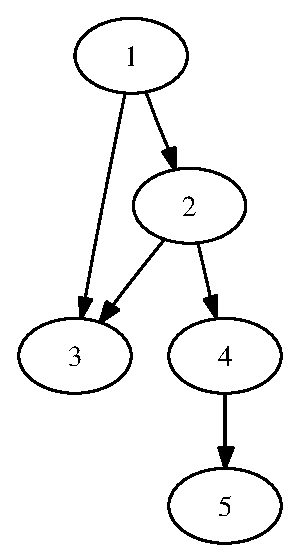
\epsfig{file=Figures/graph0,scale=0.6}

  \caption{A simple graph.}
  \label{fig:graph0}
\end{figure}



\noindent
The graph given by the relation \texttt{R} contains only the direct connections of vertices.  For example, in
the graph shown in Figure \ref{fig:graph0}, there is a direct connection from vertex $1$ to vertex $2$ and
another direct connection from vertex $2$ to vertex $4$.  Intuitively, vertex $4$ is reachable from vertex $1$,
since from vertex $1$ we can first reach vertex $2$ and from vertex $2$ we can then reach vertex $4$.  However,
there is is no direct connection between the vertices $1$ and $4$.  To make this more formal, define
a \blue{path} of a graph $R$ as a list of vertices
\\[0.2cm]
\hspace*{1.3cm}
$[x_1, x_2, \cdots, x_n]$ \quad such that \quad $\pair(x_i,x_{i+1}) \in R$ \quad for all $i=1,\cdots,n-1$.
\\[0.2cm]
In this case, the path $[x_1, x_2, \cdots, x_n]$ is written as
\\[0.2cm]
\hspace*{1.3cm}
$x_1 \mapsto x_2 \mapsto \cdots \mapsto x_n$
\\[0.2cm]
and has the \blue{length} $n-1$, since there are $n-1$ direct connections of the form $\pair(x_i,x_{i+1})$ that
make up this path.
To put it differently,  the length of a path
$[x_1,x_2,\cdots,x_n]$ is defined as the number of edges connecting the vertices and not as the
number of vertices appearing on the path.

Furthermore,  two vertices $a$ and $b$ of a graph are said to be \blue{connected} iff there exists a path
\\[0.2cm]
\hspace*{1.3cm}
$[x_1,\cdots,x_n]$ \quad such that \quad $a = x_1$ \quad and \quad $b = x_n$.
\\[0.2cm]
The goal of this section is to develop an algorithm that checks whether two vertices $a$ and $b$ are connected.
Furthermore, we want to be able to compute the corresponding path connecting the vertices $a$ and $b$.


\subsection{Computing the Transitive Closure of a Relation}
We have already noted that a graph can be represented as the set of its edges and hence as a \blue{binary relation}.
We have previously defined a \blue{binary relation} as a set of pairs.  We also need the notion of a \blue{relational product}:
If $Q$ and $R$ are binary relations, then the \blue{relational product} $Q \circ R$ of $Q$ and $R$ is defined as
\\[0.2cm]
\hspace*{1.3cm}
$Q \circ R := \Bigl\{ \pair(x, z) \Bigm| \exists y:\bigl(\pair(x,y) \in Q \wedge \pair(y,z) \in R\bigr) \Bigr\}$.
\\[0.2cm]
Furthermore, for any $n \in \mathbb{N}^*$ we can define the $n$-th power $R^n$ of the relation $R$ by induction.
\begin{description}
\item[Base Case:] $n = 1$.

             $R^1 := R$
\item[Induction Step:] $n \mapsto n+1$ 

             $R^{n+1} := R^n \circ R$.
\end{description}
The idea behind this definition is that if $\pair(x, z) \in R^n$, then there is a path of length $n$ that
starts in $x$ and ends in $z$.

In order to decide whether there is a path connecting two vertices we have to compute the 
\href{https://en.wikipedia.org/wiki/Transitive_closure}{transitive closure} $R^+$ of a relation $R$.  
To understand this notion, we first need to define the concept of \blue{transitivity}:  A relation $R$ is
transitive if and only if the following holds:
\\[0.2cm]
\hspace*{1.3cm}
$\pair(x,y) \in T \wedge \pair(y, z) \in T \rightarrow \pair(x, z) \in T$ \quad for all $x,y,z$. 
\\[0.2cm]
Now the \blue{transitive closure} $R^+$ of a binary relation $R$ is the \blue{smallest} relation $T$ such that the following
conditions hold:
\begin{itemize}
\item $R$ is a subset of $T$, i.e. we have $R \subseteq T$.
\item $T$ is transitive.
\end{itemize}
The lecture on
\href{https://github.com/karlstroetmann/Lineare-Algebra/blob/master/Skript/lineare-algebra.pdf}{Lineare Algebra} 
gives a prove that the transitive closure $R^+$ of a binary relation can be computed as follows:
\\[0.2cm]
\hspace*{1.3cm}
$R^+ = \bigcup\limits_{n=1}^{\infty} R^n = R^1 \cup R^2 \cup R^3 \cup \cdots$  
\\[0.2cm]
Initially, this formula might look intimidating as it suggests an infinite computation.
Fortunately, it turns out that we do not have to compute the powers $R^n$ for every $n \in \mathbb{N}$.  Let me
explain the reason that allows us to cut the computation short.  
\begin{enumerate}
\item $R$ is the set of direct connections between two vertices.
\item $R^2$ is the same as $R \circ R$ and this relational product is defined as
      \\[0.2cm]
      \hspace*{1.3cm}
       $R \circ R = \bigl\{ \pair(x,z) \bigm| \exists y \colon(\pair(x,y) \in R \wedge \pair(y,z)) \in R \bigr\}$.
      \\[0.2cm]
      Hence, $R \circ R$ contains those pairs $\pair(x,z)$ that are connected via one intermediate vertex $y$,
      i.e.~there is a path of the form $x \mapsto y \mapsto z$ that connects $x$ and $z$.  This path
      has length 2.  In general, we can show by induction on $n$ that $R^n$ connect those pairs that are
      connected by a path of length $n$.  The induction step of this proof runs as follows:

      $R^{n+1}$ is defined as $R^n \circ R$ and therefore we have
      \\[0.2cm]
      \hspace*{1.3cm}
      $R^n \circ R = \{ \pair(x,z) \mid \exists y \colon \pair(x,y) \in R^n \wedge \pair(y,z) \in R \}$.
      \\[0.2cm]
      As $\pair(x,y) \in R^n$, the induction hypothesis guarantees that the vertices $x$ and $y$ are
      connected by a path of length $n$.  Hence, this 
      path has the form
      \\[0.2cm]
      \hspace*{1.3cm}
      $\underbrace{x \mapsto \cdots \mapsto y}_{\mbox{\scriptsize path of length $n$.}}$
      \\[0.2cm]
      Adding $z$ at the end of this path will produce the path
      \\[0.2cm]
      \hspace*{1.3cm}
      $\underbrace{\underbrace{x \mapsto \cdots \mapsto y}_{\mbox{\scriptsize path of length $n$.}} \mapsto z}_{\mbox{\scriptsize path of length $n+1$.}}$.
      \\[0.2cm]
      This path has a length of $n + 1$ and, furthermore, connects $x$ and $z$.  Hence $R^{n+1}$
      contains those pairs $\pair(x, z)$ that are connected by a path of length $n+1$.
\end{enumerate}
Now the important observation is the following. The set of all vertices is finite.  For the arguments sake, let
us assume there are $k$ different vertices.  But then every path that has a length of $k$ or greater must
contain at least one vertex that is visited more than once and hence this path is longer than necessary,
i.e.~there is a shorter path that connects the same vertices.  Therefore, for a finite graph with $k$ vertices,
the formula to compute the transitive closure can be simplified as follows:
\\[0.2cm]
\hspace*{1.3cm} 
$\ds R^+ = \bigcup\limits_{i=1}^{k-1} R^i$.
\\[0.2cm]
While we could use this formula as its stands, it is more efficient to use a \blue{fixed-point iteration} instead.
To this end, we prove that the transitive closure $R^+$ satisfies the following equation:
\begin{equation}
  \label{fixpunkt}
  R^+ = R \cup R^+ \circ R. 
\end{equation}
The precedence of the operator $\circ$ 
is higher than the precedence of the operator $\cup$.  Therefore, the expression $R \cup R^+ \circ R$ is
equivalent to the expression $R \cup (R^+ \circ R)$.  In order to prove equation \ref{fixpunkt} we first note
that the following  \blue{law of distributivity} holds:
\\[0.2cm]
\hspace*{1.3cm}
$\ds (P \cup Q) \circ R = (P \circ R) \cup (Q \circ R)$.
\\[0.2cm]
(A proof of this equation can be found in my lecture notes on
\href{https://github.com/karlstroetmann/Lineare-Algebra/blob/master/Skript/lineare-algebra.pdf}{linear algebra}
on page 42.)  Using this law, we can prove equation \ref{fixpunkt} algebraically.  We have:
\\[0.2cm]
\hspace*{1.3cm}
$
\begin{array}{cll}
    & R \cup R^+ \circ R \\[0.2cm]
  = & R \cup \Bigl(\bigcup\limits_{i=1}^{\infty} R^i \Bigr) \circ R \\[0.4cm]
  = & R \cup \bigl(R^1 \cup R^2 \cup R^3 \cup \cdots \bigr) \circ R \\[0.2cm]
  = & R \cup \bigl(R^1 \circ R \cup R^2 \circ R \cup R^3 \circ R \cup \cdots \bigr) \\[0.2cm]
  = & R \cup \bigl(R^2 \cup R^3 \cup  R^4 \cup \cdots \bigr)  \\[0.2cm]
  = & R^1 \cup R^2 \cup R^3 \cup  R^4 \cup \cdots  \\[0.2cm]
  = & \bigcup\limits_{i=1}^{\infty} R^i \\[0.4cm]
  = & R^+.
\end{array}
$
\\[0.2cm]
Equation  \ref{fixpunkt} can now be used to compute $R^+$ via a fixed-point iteration.
To this end, let us define a sequence of relations $(T_n)_{n \in \mathbb{N}}$ by induction on $n$:
\begin{enumerate}
\item[I.A.] $n = 0$: 

            $T_0 = R$
\item[I.S.] $n \mapsto n+1$:

            $T_{n+1} = R \cup T_n \circ R $. 
\end{enumerate}
The relation  $T_n$ can be expressed via the relation $R$, we have
\begin{enumerate}
\item $T_0 = R$.
\item $T_1 = R \cup T_0 \circ R = R \cup R \circ R = R^1 \cup R^2$.
\item$\begin{array}[t]{lcl}
       T_2  & = & R \cup T_1 \circ R \\
            & = & R \cup (R^1 \cup R^2) \circ R \\
            & = & R^1 \cup R^2 \cup R^3. \\
       \end{array}
      $
\end{enumerate}
In general, we can show by induction that
\\[0.2cm]
\hspace*{1.3cm}
$\ds T_n = \bigcup\limits_{i=1}^{n+1} R^i$
\\[0.2cm]
holds for all $n \in \mathbb{N}$.  As $R^1 = R$, the base case $n=0$ of this proof is immediate from the definition of $T_0$.
In the induction step we observe the following:
\\[0.2cm]
\hspace*{1.3cm}
$
 \begin{array}{lcll}
   T_{n+1} & = & \ds R \cup T_n \circ R & \mbox{(by definition)} \\[0.2cm]
           & = & \ds R \cup \biggl(\bigcup\limits_{i=1}^{n+1} R^i\biggr) \circ R &
                 \mbox{(by induction hypothesis)} \\[0.4cm]
           & = & \ds R \cup \left(R \cup \cdots \cup R^{n+1}\right) \circ R \\[0.2cm] 
           & = & \ds R^1 \cup R^2 \cup \cdots \cup R^{n+2}  &
                 \mbox{(by the distributivity of $\circ$ over $\cup$)} \\[0.2cm]
           & = & \ds \bigcup\limits_{i=1}^{n+2} R^i & \Box 
   \end{array}
$
\\[0.2cm]
The sequence $(T_n)_{n\in\mathbb{N}}$ has another useful property:  It is 
\blue{monotonically increasing}.  In general, a sequence of sets $(X_n)_{n\in\mathbb{N}}$ is called
\blue{monotonically increasing} iff we have
\\[0.2cm]
\hspace*{1.3cm}
$\forall n \in \mathbb{N}: X_n \subseteq X_{n+1}$,
\\[0.2cm]
i.e.~the sets $X_n$ get bigger with growing index $n$.
The monotonicity of the sequence  $(T_n)_{n \in \mathbb{N}}$ is an immediate consequence of the equation
\\[0.2cm]
\hspace*{1.3cm}
$\ds T_n = \bigcup\limits_{i=1}^{n+1} R^i$ 
\\[0.2cm]
because we have:
\\[0.2cm]
\hspace*{1.3cm}
$
\begin{array}[t]{llcl}
                & \ds T_n \subseteq T_{n+1} \\[0.2cm]
\Leftrightarrow & \ds \bigcup\limits_{i=1}^{n+1} R^i \subseteq \bigcup\limits_{i=1}^{n+2} R^i \\[0.5cm]
\Leftrightarrow & \ds \bigcup\limits_{i=1}^{n+1} R^i \subseteq \left(\bigcup\limits_{i=1}^{n+1} R^i\right) \cup R^{n+2} \\
\end{array}
$
\\[0.2cm]
If the relation  $R$ is finite, then the transitive closure $R^+$ is finite, too.  All of the sets $T_n$ 
are subsets of $R^+$ because we have
\\[0.2cm]
\hspace*{1.3cm}
$\ds T_n = \bigcup\limits_{i=1}^{n+1} R^i \subseteq \bigcup\limits_{i=1}^{\infty} R^i = R^+$ \quad for all $n \in \mathbb{N}$.
\\[0.2cm]
Hence the sets $T_n$ can not grow indefinitely.  Because of the monotonicity of the sequence 
$(T_n)_{n\in\mathbb{N}}$ it follows that there exists an index  $k \in \mathbb{N}$ such that the sets $T_n$ do
not grow any further once $n$ has reached $k$, i.e.~we have
\\[0.2cm]
\hspace*{1.3cm}
$\ds \forall n \in \mathbb{N}:( n \geq k \rightarrow T_n = T_k)$.
\\[0.2cm]
But this implies that
\\[0.2cm]
\hspace*{1.3cm}
$\ds T_n = \bigcup\limits_{i=1}^{n+1} R^i = \bigcup\limits_{i=1}^{\infty} R^i = R^+$ 
\quad holds for all $n \geq k$.
\\[0.2cm]
Therefore, the algorithm for computing  $R^+$ iterates the equation 
\\[0.2cm]
\hspace*{1.3cm}
$\ds T_{n+1} = R \cup T_n \circ R$
\\[0.2cm]
until the equation  $T_{n+1} = T_n$ is satisfied, since this implies that $T_n = R^+$.


\begin{figure}[!ht]
  \centering
\begin{Verbatim}[ frame         = lines, 
                  framesep      = 0.3cm, 
                  labelposition = bottomline,
                  numbers       = left,
                  numbersep     = -0.2cm,
                  xleftmargin   = 0.8cm,
                  xrightmargin  = 0.8cm,
                ]
    def product(R1, R2):
        'Compute the relational product of R1 and R2.'
        return { (x, z) for (x, y1) in R1 for (y2, z) in R2 if y1 == y2 }
    
    def transClosure(R):
        'Compute the transitive closure of the binary relation R.'
        T = R
        while True:
            oldT = T
            T    = product(R,T) | R
            if T == oldT:
                return T
    
    R = { (1,2), (2,3), (1,3), (2,4), (4,5) }
    print( 'R  = ', R );
    print( 'Computing the transitive closure of R:' );
    T = transClosure(R);
    print( 'R+ = ', T );
\end{Verbatim} 
\vspace*{-0.3cm}
\caption{Computing the transitive closure.}  
\label{fig:transitive-closure.py}
\end{figure} %\$

\noindent
The program 
\href{https://github.com/karlstroetmann/Logic/blob/master/Python/transitive-closure.py}{\texttt{transitive-closure.py}}
that is shown in Figure
\ref{fig:transitive-closure.py} on page \pageref{fig:transitive-closure.py} shows an implementation of this idea.
The program produces the following output:
\begin{verbatim}
    R  = {(1, 2), (1, 3), (4, 5), (2, 3), (2, 4)}
    Computing the transitive closure of R:
    R+ = {(1, 2), (1, 3), (4, 5), (1, 4), (1, 5), (2, 3), (2, 5), (2, 4)}
\end{verbatim}
The transitive closure $R^+$ of a relation $R$ has a very intuitive interpretation:
It contains all pairs $\pair(x,y)$ such that there is a path leading from 
$x$ to $y$.  
The function $\texttt{product}(R_1, R_2)$ computes the relational product $R_1\circ R_2$ 
according to the formula
\\[0.2cm]
\hspace*{1.3cm}
$R_1 \circ R_2 = \Bigl\{ \langle x, z \rangle \Bigm| \exists y:\bigl(\pair(x,y) \in R_1 \wedge \pair(y,z) \in R_2\bigr) \Bigr\}$.


\subsection{Computing the Paths}
So far, given a graph represented by a relation $R$ and two vertices $x$ and $y$, we can only check
whether there is a path leading from $x$ to $y$, but we cannot compute this path.  In this
subsection we will extend the procedure \texttt{transClosure} so that it will also compute the
corresponding path.  The main idea is to extend the notion of a relational product to the notion of
a \blue{path product}, where a \blue{path product} is defined on sets of paths.  In order to do so,
we introduce three functions for tuples.
\begin{enumerate}
\item Given a tuple $T$, the function $\texttt{first}(T)$ returns the first element of $T$: 
      \\[0.2cm]
      \hspace*{1.3cm}
      $\texttt{first}\bigl(\langle x_1,\cdots,x_m\rangle\bigr) = x_1$.
\item Given a tuple $T$, the function $\texttt{last}(T)$ returns the last element of $T$: 
      \\[0.2cm]
      \hspace*{1.3cm}
      $\texttt{last}\bigl(\langle x_1,\cdots,x_m\rangle\bigl) = x_m$.
\item If $S = \langle x_1, \cdots, x_m\rangle$ and $T = \langle y_1, \cdots, y_n \rangle$ are two tuples  such that
      $\texttt{first}(S) = \texttt{last}(S)$, we define the \blue{join} $S \oplus T$ of $S$ and $T$ as \\[0.2cm]
      \hspace*{1.3cm}
      $S \oplus T = \langle x_1, \cdots, x_m, y_2, \cdots, y_n \rangle$.
\end{enumerate}
If $\mathcal{P}_1$ and $\mathcal{P}_2$ are sets of tuples representing paths, we define the \blue{path product} of
$\mathcal{P}_1$ and $\mathcal{P}_2$ as follows: \\[0.2cm]
\hspace*{1.3cm} 
$\mathcal{P}_1 \bullet \mathcal{P}_2 = 
\bigl\{\; T_1 \oplus T_2 \mid T_1 \in \mathcal{P}_1 \wedge T_2 \in \mathcal{P}_2 \wedge \texttt{last}(T_1) = \texttt{first}(T_2) \;\bigr\}
$.

\begin{figure}[!ht]
  \centering
\begin{Verbatim}[ frame         = lines, 
                  framesep      = 0.3cm, 
                  labelposition = bottomline,
                  numbers       = left,
                  numbersep     = -0.2cm,
                  xleftmargin   = 0.8cm,
                  xrightmargin  = 0.8cm,
                ]
    def findPaths(R):
        P = R;
        while True:
            oldP = P
            P    = R | pathProduct(P, R)
            if P == oldP:
                return P

    def pathProduct(P, Q):
        return { join(S, T) for S in P for T in Q if S[-1] == T[0] }
    
    def join(S, T):
        return S + T[1:]
    
    R = { (1,2), (2,3), (1,3), (2,4), (4,5) }
    print('R = ', R)
    print('Computing all paths:' )
    P = findPaths(R)
    print('P = ', P)
\end{Verbatim} 
\vspace*{-0.3cm}
\caption{Computing all connections.}  \label{fig:path.py}
\end{figure} %\$

\begin{figure}[!ht]
  \centering
  \vspace*{-9cm}

  \epsfig{file=Figures/graph-zykl,scale=0.5}
  \vspace*{-1cm}

  \caption{A graph with a cycle.}
  \label{fig:graph-zykl}
\end{figure}

Using the notion of a \blue{path product} we are able to extend the program shown in Figure
\ref{fig:transitive-closure.py} such that it computes all paths between two vertices.
The resulting program
\href{https://github.com/karlstroetmann/Logic/blob/master/Python/path.py}{\texttt{path.py}}
is shown in Figure \ref{fig:path.py} on page \pageref{fig:path.py}.
Unfortunately, the program does not work any more if the graph is \blue{cyclic}.  A graph is defined
to be \blue{cyclic} if there is a path of length greater than $1$ that starts and ends at the same
vertex.  This path is then called a \blue{cycle}.
Figure \ref{fig:graph-zykl} on page \pageref{fig:graph-zykl} shows a cyclic graph.  This graph is
cyclic because it contains the path
\\[0.2cm]
\hspace*{1.3cm}
$\langle 1, 2, 4, 1 \rangle$
\\[0.2cm]
and this path is a cycle.
The problem with this graph is that it contains an infinite number of paths that connect the vertex
1 with the vertex 2: \\[0.2cm]
\hspace*{1.3cm}
$\langle 1, 2 \rangle$, $\langle 1, 2, 4, 1, 2 \rangle$, 
$\langle 1, 2, 4, 1, 2, 4, 1, 2 \rangle$, 
$\langle 1, 2, 4, 1, 2, 4, 1, 2, 4, 1, 2 \rangle$, $\cdots$
\\[0.2cm]
Of course, there is no point in computing a path that visits a vertex more than once as these paths
contain cycles.  Our goal is to eliminate all those paths that contain cycles.


\begin{figure}[!ht]
  \centering
\begin{Verbatim}[ numbers       = left,
                  numbersep     = -0.2cm,
                  frame         = lines, 
                  framesep      = 0.3cm, 
                  labelposition = bottomline,
                  xleftmargin   = 0.0cm,
                  xrightmargin  = 0.0cm,
                ]
    def pathProduct(P, Q):
        return { join(S, T) for S in P for T in Q
                            if S[-1] == T[0] and noCycle(S, T)
               }
    
    def noCycle(T1, T2):
        return len({ x for x in T1 }.intersection({ x for x in T2 })) == 1
\end{Verbatim} 
\vspace*{-0.3cm}
\caption{Computing the connections in a cyclic graph.}  
\label{fig:path-cyclic.py}
\end{figure} %\$

Figure \ref{fig:path-cyclic.py} on page shows how the implementation of the function
\texttt{pathProduct} has to be changed so that the resulting program
\href{https://github.com/karlstroetmann/Logic/blob/master/Python/path-cyclic.py}{\texttt{path-cyclic.py}}
works also for cyclic graphs. 
\begin{enumerate}
\item In line 2 and 3, we compute only those paths that are not cyclic.
\item Line 6 defines a function \texttt{noCycle} that tests, whether the join  $\texttt{T1} \oplus \texttt{T2}$ is cyclic.  The join
      of \texttt{T1} and \texttt{T2} is cyclic iff the tuples \texttt{T1} and \texttt{T2} have more
      than one common element.  The tuples \texttt{T1} and \texttt{T2} will always have at least one common element, as we join
      these tuples only if the last element of \texttt{T1} is equal to the first element of  \texttt{T2}.
      If there would be an another vertex common to both \texttt{T1} and \texttt{T2}, then the path
      $\texttt{T1} \oplus \texttt{T2}$ would be cyclic.
\end{enumerate}

In general, we are not really interested to compute all possible paths between two given vertices
\texttt{x} and \texttt{y}.  Instead, we just want to compute the shortest path leading from \texttt{x} to \texttt{y}.
Figure \ref{fig:find_path.py} on page \pageref{fig:find_path.py} shows the procedure \texttt{reachable}. 
This procedure takes three arguments:
\begin{enumerate}
\item \texttt{start} and \texttt{goal} are vertices of a graph.
\item \texttt{R} is a binary relation representing a directed graph.
\end{enumerate}
The call  \texttt{reachable(start, goal, R)} checks whether \texttt{start} and \texttt{goal} are connected and, furthermore,
computes the shortest path from \texttt{start} to \texttt{goal}, provided such a path exists.
The complete program can be found in the file
\href{https://github.com/karlstroetmann/Logic/blob/master/Python/find\_path.py}{\texttt{find\_path.py}}.
Next, we discuss the implementation of the procedure  \texttt{reachable}.
\begin{enumerate}
\item Line 2 initializes the set \texttt{P}.  After $n$ iterations, this set will contain all paths
      that start with the vertex \texttt{start} and that have a length of at most $n$.

      Initially, there is just the trivial path $\langle\texttt{start}\rangle$ that starts with vertex
      \texttt{start} and has length $0$.
\item Line 5 tries to extend all previously computed paths by one step.
\item Line 6 selects all those paths from the set \texttt{P} that lead to the vertex \texttt{goal}.
      These paths are stored in the set \texttt{Found}.
\item Line 7 checks whether we have indeed found a path ending at \texttt{goal}.  This is the case if
      the set \texttt{Found} is not empty.  
      In this case, we return any of these paths.
\item If we have not yet found the vertex \texttt{goal} and, furthermore, we have not been able to find
      any new paths during this iteration,  the procedure returns in line 10.
      As the \texttt{return} statement in line 11 does not return a value, the procedure will
      instead return the value \texttt{None}.
\end{enumerate}
The procedure call \texttt{reachable(start,goal R)} will compute the \textbf{shortest} path connecting
\texttt{start} and \texttt{goal} because it computes path with increasing length.  The first iteration
computes all paths starting in \texttt{start} that have a length of at most 1, the second iteration
computes all paths starting in \texttt{start} that have a length of at most 2, and in general the $n$-th
iteration computes all paths starting in \texttt{start} that have a length of at most $n$.  Hence, if
there is a path of length $n$, then this path will be found in the $n$-iteration unless a shorter path has
already been found in a previous iteration.  

\remarkEng
The algorithm described above is known as 
\href{https://en.wikipedia.org/wiki/Breadth-first_search}{breadth first search}. \eox 

\begin{figure}[!ht]
  \centering
\begin{Verbatim}[ frame         = lines, 
                  framesep      = 0.3cm, 
                  labelposition = bottomline,
                  numbers       = left,
                  numbersep     = -0.2cm,
                  xleftmargin   = 0.8cm,
                  xrightmargin  = 0.8cm,
                ]
    def reachable(start, goal, R):
        P = { (start,) }
        while True:
            oldP  = P
            P     = P | path_product(P, R)
            Found = { T for T in P if T[-1] == goal }
            if Found != set():
                return Found.pop()
            if P == oldP:
                return
                
    def path_product(P, R):
        return set( add(T1, T2) for T1 in P for T2 in R
                             if T1[-1] == T2[0] and noCycle(T1, T2)
                  )
    
    def noCycle(T1, T2):
        return len(set(T1).intersection(set(T2))) == 1
    
    def add(T, P):
        return T + (P[-1],)
\end{Verbatim} 
\vspace*{-0.3cm}
\caption{Finding the shortest path between two vertices.}  
\label{fig:find_path.py}
\end{figure}

\subsection{The Wolf, the Goat, and the Cabbage}
Next, we present an application of the theory developed so far.  We solve a problem that has puzzled
the greatest agricultural economists for centuries.  The puzzle we want to solve is known as the 
\href{http://jeux.lulu.pagesperso-orange.fr/html/anglais/loupChe/loupChe1.htm}{wolf-goat-cabbage puzzle}:  
\vspace*{0.3cm}

\begin{minipage}[c]{16cm}
{\sl
An agricultural economist has to sell a wolf, a goat, and a cabbage on a market place.  In order to
reach the market place, she has to cross a river.  The boat that she can use is so small that it can
only accommodate either the goat, the wolf, or the cabbage in addition to the agricultural economist.
Now if the agricultural economist leaves the wolf alone with the goat, the wolf will eat the goat.
If, instead, the agricultural economist leaves the goat with the cabbage, the goat will eat the cabbage.
Is it possible for the agricultural economist to develop a schedule that allows her to cross the river
without either the goat or the cabbage being eaten?
}
\end{minipage}
\vspace*{0.3cm}

\noindent
In order to compute a schedule, we first have to model the problem.  The various \blue{states} of the problem will
be regarded as \blue{vertices} of a graph and this graph will be represented as a binary relation.
To this end we define the set
\begin{verbatim}
  All = {'farmer', 'wolf, 'goat', 'cabbage'}
\end{verbatim}
Every node will be represented as a subset \texttt{S} of the set \texttt{All}.  The idea is that the set \texttt{S}
specifies those objects that are on the left side of the river.  We assume that initially the farmer and his goods
are on the left side of the river. 
Therefore, the set of all possible states can be defined as the set
\begin{verbatim}
  States = {S for S in power(All) if not problem(S) and not problem(All-S)}
\end{verbatim}
Here, we have used the procedure \texttt{problem} to check whether a given set \texttt{S} has a problem. 
Note that since \texttt{S} is the set of objects on the left side, the expression $\texttt{All-S}$
computes the set of objects on the right side of the river.

Next, a set \texttt{S} of objects has a problem if both of the following conditions
are satisfied:
\begin{enumerate}
\item The farmer is not an element of \texttt{S} and
\item either \texttt{S} contains both the goat and the cabbage or \texttt{S} contains both the wolf and the goat.
\end{enumerate}
Therefore, we can implement the function \texttt{problem} as follows:
\begin{verbatim}
  def problem(S):
      return ('farmer' not in S) and             \
             (('goat' in S and 'cabbage' in S) or   # goat eats cabbage
              ('wolf' in S and 'goat'    in S)   )  # wolf eats goat
\end{verbatim}
We proceed to compute the relation \texttt{R} that contains all possible transitions between
different states.  We will compute \texttt{R} using the formula:
\\[0.2cm]
\hspace*{0.75cm}
\texttt{R = R1 + R2;}
\\[0.2cm]
Here \texttt{R1} describes the transitions that result from the farmer crossing the river from left
to right, while \texttt{R2} describes the transitions that result from the farmer crossing the river
from right to left.  We can define the relation \texttt{R1} as follows:
\begin{verbatim}
  R1 = { (S, S-B) for S in States for B in power(S)
                  if S-B in States and 'farmer' in B and len(B) <= 2
       }
\end{verbatim}
Let us explain this definition in detail:
\begin{enumerate}
\item Initially, \texttt{S} is the set of objects on the left side of the river.  Hence, \texttt{S}
      is an element of the set of all states that we have defined as \texttt{P}.
\item \texttt{B} is the set of objects that are put into the boat and that do cross the river.  Of
      course, for an object to go into the boat is has to be on the left side of the river to begin
      with.  Therefore, \texttt{B} is a subset of \texttt{S} and hence an element of the power set
      of \texttt{S}. 
\item Then  \texttt{S-B} is the set of objects that are left on the left side of the river after
      the boat has crossed.  Of course, the new state \texttt{S-B} has to be a state that does not
      have a problem.  Therefore, we check that \texttt{S-B} is an element of \texttt{States}.
\item Furthermore, the farmer has to be inside the boat.  This explains the condition 
      \\[0.2cm]
      \hspace*{1.3cm}
      \texttt{\symbol{39}farmer\symbol{39} in B}.
\item Finally, the boat can only have two passengers.  Therefore, we have added the condition
      \\[0.2cm]
      \hspace*{1.3cm}
      \texttt{len(B) <= 2}.
\end{enumerate}
Next, we have to define the relation \texttt{R2}.  However, as crossing the river from right to left
is just the reverse of crossing the river from left to right, \texttt{R2} is just the \blue{inverse} of
\texttt{R1}.   Hence we define:
\begin{verbatim}
  R2 = { (S2, S1) for (S1, S2) in R1 }
\end{verbatim}
Next, the relation \texttt{R} is the union of \texttt{R1} and \texttt{R2}:
\begin{verbatim}
  R = R1 | R2
\end{verbatim}
Finally, the start state has all objects on the left side.  Therefore, we have
\begin{verbatim}
  start = All
\end{verbatim}
In the end, all objects have to be on the right side of the river.  That means that nothing is left
on the left side.  Therefore, we define
\begin{verbatim}
  goal = {}
\end{verbatim}


\begin{figure}[h]
  \centering

  \epsfig{file=Figures/wolf-goat-cabbage, scale=0.4}

  \caption{The relation \texttt{R} shown as a directed graph.}
  \label{fig:wolf-goat-cabbage.pdf}
\end{figure}




Figure \ref{fig:wolf-ziege} on page \pageref{fig:wolf-ziege} shows the program
\href{https://github.com/karlstroetmann/Logic/blob/master/Python/wolf-goat-cabbage.py}{\texttt{wolf-goat-cabbage.py}}
that combines the statements shown so far.  The solution computed by this program is shown in Figure
 \ref{fig:wolf-ziege-solution}.

\begin{figure}[!ht]
  \centering
\begin{Verbatim}[ codes         = {\catcode`$=3\catcode`_=8\catcode`^=7},
                  frame         = lines, 
                  framesep      = 0.3cm, 
                  labelposition = bottomline,
                  numbers       = left,
                  numbersep     = -0.2cm,
                  xleftmargin   = 0.3cm,
                  xrightmargin  = 0.3cm,
                ]
    def problem(S):
        return ('farmer' not in S) and             \
               (('goat' in S and 'cabbage' in S) or   # goat eats cabbage
                ('wolf' in S and 'goat'    in S)   )  # wolf eats goat
    
    All   = frozenset( {'farmer', 'wolf', 'goat', 'cabbage'} )
    R1    = { (S, S - B) for S in States for B in power(S)
                         if S - B in States and 'farmer' in B and len(B) <= 2
            }
    R2    = { (S2, S1) for (S1, S2) in R1 }
    R     = R1 | R2
    start = All
    goal  = frozenset()
    Path  = findPath(start, goal, R)
\end{Verbatim} 
\vspace*{-0.3cm}
\caption{Solving the wolf-goat-cabbage problem.}  
\label{fig:wolf-ziege}
\end{figure}


\begin{figure}[!ht]
  \centering
\begin{Verbatim}[ codes         = {\catcode`$=3\catcode`_=8\catcode`^=7},
                  frame         = lines, 
                  framesep      = 0.3cm, 
                  labelposition = bottomline,
                  numbers       = left,
                  numbersep     = -0.2cm,
                  xleftmargin   = 0.8cm,
                  xrightmargin  = 0.8cm,
                ]
    {'cabbage', 'farmer', 'goat', 'wolf'}                                 {}
                             >>>> {'farmer', 'goat'} >>>> 
    {'cabbage', 'wolf'}                                   {'farmer', 'goat'}
                             <<<< {'farmer'} <<<< 
    {'cabbage', 'farmer', 'wolf'}                                   {'goat'}
                             >>>> {'farmer', 'wolf'} >>>> 
    {'cabbage'}                                   {'farmer', 'goat', 'wolf'}
                             <<<< {'farmer', 'goat'} <<<< 
    {'cabbage', 'farmer', 'goat'}                                   {'wolf'}
                             >>>> {'cabbage', 'farmer'} >>>> 
    {'goat'}                                   {'cabbage', 'farmer', 'wolf'}
                             <<<< {'farmer'} <<<< 
    {'farmer', 'goat'}                                   {'cabbage', 'wolf'}
                             >>>> {'farmer', 'goat'} >>>> 
    {}                                 {'cabbage', 'farmer', 'goat', 'wolf'}
\end{Verbatim} 
\vspace*{-0.3cm}
\caption{A schedule for the agricultural economist.}  
\label{fig:wolf-ziege-solution}
\end{figure}
\pagebreak
\vspace*{\fill}



\section{Symbolic Differentiation}
In this section we will develop a program that reads an arithmetic expression like 
\\[0.2cm]
\hspace*{1.3cm}
\texttt{\symbol{34}x * exp(x)\symbol{34}},
\\[0.2cm]
interprets this string as describing the real valued function 
\\[0.2cm]
\hspace*{1.3cm}
$x \mapsto x \cdot \exp(x)$, 
\\[0.2cm]
and then takes the derivative of this function with respect to the variable $x$.  In order to specify the input
of this program more clearly, we first define the notion of an \blue{arithmetic expression} inductively.
\begin{enumerate}
\item Every number $c \in \mathbb{R}$ is an arithmetic expression.
\item Every variable $v$ is an arithmetic expression.
\item If $s$ and $t$ are arithmetic expressions, then
      \\[0.2cm]
      \hspace*{1.3cm}
      $s + t$, \quad $s - t$, \quad $s * t$, \quad $s / t$, \quad and \quad $s \,\mathtt{**}\, t$
      \\[0.2cm]
      are arithmetic expressions.  Here $s \,\mathtt{**}\, t$ is interpreted as $s^t$.
      
\item If $e$ is an arithmetic expression, then both
      \\[0.2cm]
      \hspace*{1.3cm}
      $\exp(e)$ \quad and \quad $\ln(e)$
      \\[0.2cm]
      are arithmetic expressions.
\end{enumerate}
We want do implement a function \texttt{diff} that takes two arguments:
\begin{enumerate}
\item The first argument \texttt{expr} is an arithmetic expression.
\item The second argument \texttt{var} is the name of a variable.
\end{enumerate}
The function call \texttt{diff(expr, var)} will then compute the derivative of \texttt{expr} with respect to the variable \texttt{var}.  For example, the function call \texttt{diff(\symbol{34}x*exp(x)\symbol{34}, \symbol{34}x\symbol{34})} will compute the output
\\[0.2cm]
\hspace*{1.3cm}
\symbol{34}\texttt{1*exp(x) + x*exp(x)}\symbol{34}
\\[0.2cm]
because we have:
$$ \frac{\mathrm{d}\;}{\mathrm{d}x} \bigl( x \cdot \mathrm{e}^x \bigr) = 1 \cdot x + x \cdot \mathrm{e}^x $$
It would be very tedious to \blue{represent} arithmetic expressions as strings.  Instead, we will represent
arithmetic expressions as \blue{nested tuples}.  The notion of a \emph{nested tuple} is defined inductively:
\begin{itemize}
\item $\langle x_1, x_2, \cdots, x_n \rangle$ is a nested tuple if each of the components $x_i$ is either a
      number, a string, or is itself a nested tuple.
\end{itemize}
For example, the arithmetic expression ``\texttt{x*exp(x)}'' is represented as the nested tuple
\\[0.2cm]
\hspace*{1.3cm}
$\bigl\langle\texttt{\symbol{34}}*\texttt{\symbol{34}}, \texttt{\symbol{34}}x\texttt{\symbol{34}}, \langle \texttt{\symbol{34}}\mathtt{exp}\texttt{\symbol{34}}, \texttt{\symbol{34}}x\texttt{\symbol{34}} \rangle\bigr\rangle$.
\\[0.2cm]
In order to be able to convert string into nested tuples, we need a \blue{parser}.  A parser is a program that
takes a string as input and transforms this string into a nested tuple, which is then returned as a result.
I have implemented a parser in the file ``\texttt{exprParser.py}''.  The details of the implementation of this
parser will be discussed in the lecture on algorithms.

\noindent
The function \texttt{diff} that is shown in Figure \ref{fig:diff.py} on page \pageref{fig:diff.py} is part
of the program
\href{https://github.com/karlstroetmann/Logic/blob/master/Python/diff.py}{\texttt{diff.py}}.
This function is called with one argument:
The argument \texttt{e} is an arithmetic expression.
The function \texttt{diff} interprets its argument \texttt{e} as a function of the variable
\texttt{x}.  We take the \href{https://en.wikipedia.org/wiki/Derivative}{derivative} of this
function with respect to the variable \texttt{x}.  For example, in order to compute the derivative of
the function
\\[0.2cm]
\hspace*{1.3cm}
$x \mapsto x^x$,
\\[0.2cm]
we can call the function  \texttt{diff} as follows:
\\[0.2cm]
\hspace*{1.3cm}
\texttt{diff(\symbol{34}x ** x\symbol{34})}.
\\[0.2cm]
Let us now discuss the implementation of the function \texttt{diff} in more detail.  
\begin{enumerate}
\item The lines 3 - 6 implement the rule: 
      $$\frac{\mathrm{d}\;}{\mathrm{d}x}\bigl(f(x) + g(x)\bigr) = \frac{\mathrm{d}\;}{\mathrm{d}x} f(x) + \frac{\mathrm{d}\;}{\mathrm{d}x} g(x)$$
\item Line 7 - 10 implement the rule:
      $$\frac{\mathrm{d}\;}{\mathrm{d}x}\bigl(f(x) - g(x)\bigr) = \frac{\mathrm{d}\;}{\mathrm{d}x} f(x) - \frac{\mathrm{d}\;}{\mathrm{d}x} g(x)$$      
\item Line 11 - 14 deals with the case where \texttt{e} is a product.  The 
      \href{https://en.wikipedia.org/wiki/Product\_rule}{product rule} is      
      $$ \frac{\mathrm{d}\;}{\mathrm{d}x}\bigl(f(x) \cdot g(x)\bigr) = \left(\frac{\mathrm{d}\;}{\mathrm{d}x} f(x)\right)\cdot g(x) + f(x) \cdot \left(\frac{\mathrm{d}\;}{\mathrm{d}x} g(x)\right)
      $$
\item Line 15 - 17 deals with the case where \texttt{e} is a quotient.  The
      \href{https://en.wikipedia.org/wiki/Quotient\_rule}{quotient rule} is
      $$ \frac{\mathrm{d}\;}{\mathrm{d}x}\left(\frac{f(x)}{g(x)}\right) = 
         \frac{\displaystyle\left(\frac{\mathrm{d}\;}{\mathrm{d}x} f(x)\right)\cdot g(x) - 
         f(x) \cdot \left(\frac{\mathrm{d}\;}{\mathrm{d}x} g(x)\right)}{g(x) \cdot g(x)}
      $$      
\item Line 19 - 21 deals with the case where \texttt{e} is a power.  Now in order to take the derivative of an
      expression of the form
      $$  f(x)^{g(x)} $$
      we first need to rewrite this expression using the following trick:
      $$ f(x)^{g(x)} = \exp\bigl(\ln\bigl(f(x)^{g(x)}\bigr)\bigr) = \exp\bigl(g(x) \cdot \ln(f(x))\bigr) $$
      Then, we can recursively call \texttt{diff} for this expression.  This works, because the function
      \texttt{diff} can deal with both the exponential function $x \mapsto \exp(x)$ and with the natural
      logarithm $x \mapsto \ln(x)$.  This rewriting is done in line 21.      
\item Line 22-25 deals with the case where \texttt{e} has the form 
      $$\ln\bigl(f(x)\bigr)$$  
      In order to take the derivative of this expression, we first need to know the derivative of the natural
      logarithm.  This derivative is given as     
      $$ \frac{\mathrm{d}\;}{\mathrm{d}x} \ln(x) = \frac{1}{x}$$
      Then, using the \href{https://en.wikipedia.org/wiki/Chain\_rule}{chain rule} we have that
      $$ \frac{\mathrm{d}\;}{\mathrm{d}x} \ln\bigl(f(x)\bigr) = \frac{\frac{\mathrm{d}\;}{\mathrm{d}x} f(x)}{f(x)}$$     
\item Line 26 - 29 deals with the case where \texttt{e} has the form $\exp\bigl(f(x)\bigr)$.  
      In order to take the derivative of this expression, we first need to know the derivative of the 
      \href{https://en.wikipedia.org/wiki/Exponential\_function}{exponential function}.  
      This derivative is given as 
      $$ \frac{\mathrm{d}\;}{\mathrm{d}x} \exp(x) = \exp(x)$$    
      Then, using the \href{https://en.wikipedia.org/wiki/Chain\_rule}{chain rule} we have that
      $$\frac{\mathrm{d}\;}{\mathrm{d}x} \exp\bigl(f(x)\bigr) = \left(\frac{\mathrm{d}\;}{\mathrm{d}x} f(x)\right) \cdot \exp\bigl(f(x)\bigr) $$
\item Line 30-31 deals with the case where \texttt{e} is a variable and happens to be the same variable as
      \texttt{x}.  This is checked using the condition    
      \texttt{e == x}.  As we have
      $$\frac{\mathrm{d}x}{\mathrm{d}x} = 1,$$
      the function \texttt{diff} returns \texttt{1} in this case.  
\item Otherwise, the expression is assumed to be a constant and hence we return 0.
\end{enumerate}


\begin{figure}[!ht]
\centering
\begin{Verbatim}[ frame         = lines, 
                  framesep      = 0.3cm, 
                  firstnumber   = 1,
                  labelposition = bottomline,
                  numbers       = left,
                  numbersep     = -0.2cm,
                  xleftmargin   = 0.8cm,
                  xrightmargin  = 0.8cm,
                ]
    def diff(e):
        'differentiate the expressions e with respect to the variable x'
        if e[0] == '+':
            f , g  = e[1:]
            fs, gs = diff(f), diff(g)
            return ('+', fs, gs)
        if e[0] == '-':
            f , g  = e[1:]
            fs, gs = diff(f), diff(g)
            return ('-', fs, gs)
        if e[0] == '*':
            f , g  = e[1:]
            fs, gs = diff(f), diff(g)
            return ('+', ('*', fs, g), ('*', f, gs))
        if e[0] == '/':
            f , g  = e[1:]
            fs, gs = diff(f), diff(g)
            return ('/', ('-', ('*', fs, g), ('*', f, gs)), ('*', g, g))
        if e[0] == '**':
            f , g  = e[1:]
            return diff(('exp', ('*', g, ('ln', f))))
        if e[0] == 'ln':
            f  = e[1]
            fs = diff(f) 
            return ('/', fs, f)
        if e[0] == 'exp':
            f  = e[1]
            fs = diff(f) 
            return ('*', fs, e)
        if e == 'x':
            return '1'
        return 0                  
\end{Verbatim}
\vspace*{-0.3cm}
\caption{A function for symbolic differentiation}
\label{fig:diff.py}
\end{figure}


In order to test this function we can implement a function \texttt{test} as shown in Figure \ref{fig:test-diff.py}.
Then the expression
\\[0.2cm]
\hspace*{1.3cm}
\texttt{diff(\symbol{34}x ** x\symbol{34})}
\\[0.2cm]
yields the result:
\\[0.2cm]
\hspace*{1.3cm}
d/dx x ** x = (1*ln(x) + x*1/x)*exp(x*ln(x))
\\[0.2cm]
This shows that
\\[0.2cm]
\hspace*{1.3cm}
$\ds \frac{\mathrm{d}\;}{\mathrm{d}x} x^x = \bigl(\ln(x) + 1\bigr) \cdot \exp\bigl(x \cdot \ln(x)\bigr) =
 \bigl(\ln(x) + 1\bigr) \cdot x^x
$.


\begin{figure}[!ht]
\centering
\begin{Verbatim}[ frame         = lines, 
                  framesep      = 0.3cm, 
                  firstnumber   = 1,
                  labelposition = bottomline,
                  numbers       = left,
                  numbersep     = -0.2cm,
                  xleftmargin   = 0.8cm,
                  xrightmargin  = 0.8cm,
                ]
    import exprParser as ep

    def test(s):
        t = ep.ExprParser(s).parse()
        d = diff(t)
        print(f'd/dx {s} = {ep.toString(d)}')
\end{Verbatim}
\vspace*{-0.3cm}
\caption{Testing symbolic differentiation.}
\label{fig:test-diff.py}
\end{figure}





%%% Local Variables:
%%% mode: latex
%%% TeX-master: "logic"
%%% End:

\chapter{Grenzen der Berechenbarkeit}
\section{Das Halte-Problem}
In diesem Abschnitt werden wir eine konkrete Funktion angeben, die
nicht durch ein \texttt{C}-Programm implementiert werden kann.  Vorweg geben wir eine Definition, die
wir ben"otigen, um das Halte-Problem konkret formulieren zu k"onnen.
\begin{Definition}[Test-Funktion] {\em Ein String $t$ ist eine \emph{Test-Funktion} mit Namen $n$ wenn $t$ ein
String der Form \\[0.3cm]
\hspace*{1.3cm} {\tt int $n$(char* x) \{ $\cdots$ \}} \\[0.3cm]
ist, der sich als Definition einer $C$-Funktion parsen l"a\3t.  Die Menge der
Test-Funktionen bezeichnen wir mit $T\!F$.  Ist $t \in T\!F$ und hat den Namen $n$, so
schreiben wir $\mathtt{name}(t) = n$.} \hspace*{\fill} $\Box$
\end{Definition}

\noindent
\textbf{Beispiele}:  
\begin{enumerate}
\item $s_1$ = ``{\tt int simple(char* x) \{ return 0; \}}''

      $s_1$ ist eine (sehr einfache) Test-Funktion mit dem Namen \texttt{simple}.
\item $s_2$ = ``{\tt int loop(char* x) \{ while (1) ++x; \}}''

      $s_2$ ist eine Test-Funktion mit dem Namen \texttt{loop}. 
\item $s_3$ = ``{\tt int loop(char* x);}''

      $s_3$ ist keine Test-Funktion, denn es ist lediglich eine Deklaration einer
      \texttt{C}-Funktion und keine Definition.
\item $s_4$ = ``{\tt int hugo(char* x) begin i := 1; end;}''

      $s_4$ ist keine Test-Funktion, denn es l"a\3t sich mit einem
      \texttt{C}-Compiler nicht fehlerfrei parsen.
\item $s_5$ = ``{\tt int hugo(int x) \{ return i*i; \}}''

      $s_5$ ist auch keine Test-Funktion, denn der Typ des Arguments ist \texttt{int}
      und nicht \texttt{char*}.
\end{enumerate}
Um das Halte-Problem "ubersichtlicher formulieren zu k"onnen, f"uhren wir noch drei
zus"atzliche Notationen ein.
\begin{Notation}[$\leadsto$, $\downarrow$, $\uparrow$]
{\em
Ist $n$ der Name einer \texttt{C}-Funktion und sind $a_1$, $\cdots$, $a_n$ Argumente, die
vom Typ her der Deklaration von $n$ entsprechen, so schreiben wir \\[0.3cm]
\hspace*{1.3cm} $n(a_1, \cdots, a_n) \leadsto r$ \\[0.3cm]
wenn der Aufruf $n(a_1, \cdots, a_n)$ das Ergebnis $r$ liefert.  Sind wir an dem Ergebnis
selbst nicht interessiert, sondern wollen nur angeben, da\3 ein Ergebnis existiert, so
schreiben wir \\[0.3cm]
\hspace*{1.3cm} $n(a_1, \cdots, a_n) \,\downarrow$ \\[0.3cm]
Terminiert der Aufruf $n(a_1, \cdots, a_n)$ nicht, so schreiben wir \\[0.3cm]
\hspace*{1.3cm} $n(a_1, \cdots, a_n) \,\uparrow$ \hspace*{\fill} $\Box$
}
\end{Notation}

\noindent
\textbf{Beispiele}: Legen wir die Funktions-Definitionen zugrunde, die wir im Anschlu\3 an
die Definition des Begriffs der Test-Funktion gegeben haben, so gilt:
\begin{enumerate}
\item {\tt simple(\symbol{34}emil\symbol{34}) $\leadsto 0$}
\item {\tt simple(\symbol{34}emil\symbol{34}) $\downarrow$}
\item {\tt loop(\symbol{34}hugo\symbol{34}) $\uparrow$}
\end{enumerate}

\noindent
Wir betrachten jetzt ein \texttt{C}-Funktion \texttt{stops}, die folgende Deklaration
hat:
\begin{verbatim}
      int stops(char* t, char* a);
\end{verbatim}
Wir nehmen einmal an, dass es eine Implementierung dieser Funktion g"abe, die das Halte-Problem l"ost.  Genauer sagen wir, dass
f"ur den Aufruf \texttt{stops($t$, $a$)} folgendes gelten soll:
\begin{enumerate}
\item $t \not\in T\!F \quad\rightarrow\quad \mathtt{stops}(t, a) \leadsto 2$.

      In Worten: Wenn $t$ keine Test-Funktion ist, dann liefert der Aufruf \\
      \texttt{stops($t$, $a$)} den Wert 2 zur"uck.
\item $t \in T\!F \,\wedge\, \mathtt{name}(t) = n \,\wedge\, n(a)\downarrow \quad\rightarrow\quad
       \mathtt{stops}(t, a) \leadsto 1$.

      In Worten: Wenn $t$ eine Test-Funktion mit Namen $n$ ist und der Aufruf $n(a)$ terminiert,
      dann liefert der Aufruf \texttt{stops($t$, $a$)} den Wert 1 zur"uck.
\item $t \in T\!F \,\wedge\, \mathtt{name}(t) = n \,\wedge\, n(a)\uparrow \quad\rightarrow\quad
       \mathtt{stops}(t, a) \leadsto 0$.

      In Worten: Wenn $t$ eine Test-Funktion mit Namen $n$ ist und der Aufruf $n(a)$ \underline{nicht} terminiert,
      dann liefert der Aufruf \texttt{stops($t$, $a$)} den Wert 0 zur"uck. 
\end{enumerate}

Als n"achstes betrachten wir eine etwas seltsame Test-Funktion, die den Namen
\texttt{strange} tr"agt. Diese Funktion ist in Abbildung \ref{fig:strange} zu sehen.
Die Zeilen in der Abbildung sind numeriert.  Diese Zeilennummern sind aber nicht Teil der
\texttt{C}-Funktion und dienen nur der folgenden Erl"auterung.
\begin{figure}[!h]
\begin{verbatim}
 01   int strange(char* x) {
 02       int result;
 03       result = stops(x, x);
 04       if (result == 1) 
 05           while (1) 
 06               ++result;
 07       return result;
 08   }
\end{verbatim}
  \caption{Die Test-Funktion \texttt{strange}.}
  \label{fig:strange}
\end{figure}

Zun"achst "uberzeugen wir uns davon, dass die abgebildete Funktion sich als $C$-Funktion parsen
l"a\3t.  Dies k"onnen wir beispielsweise dadurch tun, dass wir die Funktion mit einem
\texttt{C}-Compiler "ubersetzen.  Als n"achstes bezeichnen wir den String in Abbildung 
\ref{fig:strange} mit $Strange$.  Wir definieren also \\[0.3cm]
\hspace*{1.3cm} $Strange$ = ``{\tt int strange(char* x) \{} \\
\hspace*{3.8cm}  {\tt       int result;} \\
\hspace*{3.8cm}  {\tt       result = stops(x, x);} \\
\hspace*{3.8cm}  {\tt       if (result == 1) } \\
\hspace*{4.3cm}  {\tt           while (1) } \\
\hspace*{4.8cm}  {\tt               ++result;} \\
\hspace*{3.8cm}  {\tt       return result;} \\
\hspace*{3.3cm}  {\tt   \}}'' \\[0.3cm]
und stellen fest, dass gilt: \\[0.3cm]
\hspace*{1.3cm} $Strange \in T\!F \;\wedge\; \mathtt{name}(Strange) = \mathtt{strange}$. \\[0.3cm]
Damit sind wir in der Lage, den String $Strange$ als Eingabe der Funktion \texttt{stops}
zu verwenden.  Wir betrachten nun den folgenden Aufruf: \\[0.3cm]
\hspace*{1.3cm} \texttt{stops($Strange$, $Strange$)}. \\[0.3cm]
Es k"onnen drei F"alle auftreten:
\begin{enumerate}
\item $\mathtt{stops}(Strange, Strange) \leadsto 0$. 

      Nach der Spezifikation von \texttt{stops} bedeutet dies \\[0.3cm]
      \hspace*{1.3cm} $\mathtt{strange}(Strange) \uparrow$ \\[0.3cm]
      Schauen wir nun, was wirklich beim Aufruf \texttt{strange($Strange$)} passiert:
      In Zeile 3 erh"alt die Variable \texttt{result} den Wert 0 zugewiesen.  In Zeile 4
      wird dann getestet, ob \texttt{result} den Wert 1 hat.  Dieser Test schl"agt fehl.
      Daher wird der Block der \texttt{if}-Anweisung nicht ausgef"uhrt und die Funktion liefert als
      n"achstes in Zeile 7 den Wert 0 zur"uck.  Insbesondere terminiert der Aufruf also, im
      Widerspruch zu dem, was die Funktion \texttt{stops} behauptet hat.
\item  $\mathtt{stops}(Strange, Strange) \leadsto 1$. 

      Aus der Spezifikation der Funktion \texttt{stops} folgt: \\[0.3cm]
      \hspace*{1.3cm} $\mathtt{strange}(Strange) \downarrow$ \\[0.3cm]
      Schauen wir nun, was wirklich beim Aufruf \texttt{strange($Strange$)} passiert:
      In Zeile 3 erh"alt die Variable \texttt{result} den Wert 1 zugewiesen.  In Zeile 4
      wird dann getestet, ob \texttt{result} den Wert 1 hat.  Diesmal gelingt der Test.
      Daher wird der Block der \texttt{if}-Anweisung ausgef"uhrt.  Dieser Block
      besteht aber nur aus einer Endlos-Schleife, aus der wir nie wieder zur"uck kommen.
      Das steht im Widerspruch zu dem, was die Funktion \texttt{stops} behauptet hat.
\item  $\mathtt{stops}(Strange, Strange) \leadsto 2$. 

      Dann m"u\3te aber der Programmtext $Strange$ einen Syntax-Fehler enthalten, was nicht
      der Fall ist.
\end{enumerate}
Insgesamt haben wir also in jedem Fall einen Widerspruch erhalten.  
Wir haben diesen Widerspruch aus der Annahme erhalten, dass die \texttt{C}-Funktion \texttt{stops}
das Halte-Problem l"ost.  Daher haben wir gezeigt, dass es keine \texttt{C}-Funktion
geben kann, die das Halte-Problem l"ost.

An dieser Stelle k"onnen wir uns fragen, ob es vielleicht eine andere Programmier-Sprache
gibt, in der wir das Halte-Problem dann vielleicht doch l"osen k"onnten.  
Wenn es in dieses Programmier-Sprache Unterprogramme gibt, und wenn wir dort
Programm-Texte als Argumente von Funktionen "ubergeben k"onnen, dann ist leicht zu sehen,
dass der obige Beweis der 
Unl"osbarkeit des Halte-Problems sich durch geeignete syntaktische Modifikationen auch auf
die andere Programmier-Sprache "ubertragen l"a\3t.

\section{Die Church'sche These}
In diesem Zusammenhang sollten wir noch die \emph{Church'sche These}\footnote{
Diese These wurde 1936 von Alonzo Church (1903-1995) aufgestellt.} erw"ahnen.  F"ur unsere Zwecke k"onnen wir diese wie folgt formulieren:
\begin{center}
\begin{tabular}{|l|}
 \hline
 \hline
    \rule{0pt}{14pt}
    Ist $f$ eine Funktion die wir mit einer beliebigen, geeigneten \\
    Programmier-Sprache berechnen k"onnen, so k"onnen wir $f$ \\
        auch durch ein geeignetes  \texttt{C}-Programm 
    berechnen.     
    \rule[-6pt]{0pt}{14pt}
    \\
 \hline
 \hline
\end{tabular}
\end{center}
Es kann nat"urlich durchaus sein, dass eine bestimmte Programmier-Sprache wesentlich
geeigneter ist, um ein gegebenes Problem zu l"osen.  F"ur ein gegebenes Problem ist es
leicht m"oglich, dass das \texttt{C}-Programm deutlich l"anger und komplizierter
ist, als ein Programm, das in einer geeigneteren Sprache entwickelt wird.  Nur gibt es
eben kein l"osbares Problem, das wir nicht schon in \texttt{C} l"osen k"onnen, auch wenn das
vielleicht viel m"uhsamer ist als in einer anderen Sprache.

Die Church'sche These ist ihrer Natur nach nicht formal beweisbar, weil jeder Beweis eine
irgendwie geartete Formalisierung des Berechenbarkeits-Begriffs voraussetzen w"urde.  
In der Literatur wird die Church'sche These in der Regel nicht durch Bezug auf die
Programmier-Sprache \texttt{C} formuliert. Stattdessen greift man dort auf den Begriff der
\emph{Turing-Berechenbarkeit}  zur"uck.  Diesem Begriff liegt das Konzept eines sehr
primitiven Computers zugrunde, der sogenannten \emph{Turing-Maschine}\footnote{
Dieses Modell eines Computers geht auf Alan Turing (1912-1954) zur"uck.}.
  Die Tatsache, dass es nie gelungen ist Programmier-Sprachen
zu entwickeln, die mehr berechnen k"onnen als eine Turing-Maschine berechnen kann, hat
zur allgemeinen Akzeptanz der Church'schen These gef"uhrt.

\section{Andere nicht berechenbare Funktionen}
Es gibt noch eine ganze Reihe anderer Funktionen, die nicht berechenbar sind.  In der
Regel werden wir den Nachweis, dass eine bestimmt Funktion nicht berechenbar ist dadurch f"uhren, dass
wir zun"achst annehmen, dass die gesuchte Funktion doch implementierbar ist.  Unter dieser Annahme
konstruieren wir dann eine Funktion, die das Halte-Problem l"ost, was im Widerspruch zu dem am Anfang dieses Abschnitts
bewiesen Sachverhalts steht.
Dieser Widerspruch zwingt uns zu der Folgerung, dass die gesuchte Funktion nicht implementierbar ist.
Wir werden dieses Verfahren an einem Beispiel demonstrieren. Vorweg ben"otigen wir aber
noch eine Definition.

\begin{Definition}[$\simeq$] 
{\em 
Es seien $n_1$ und $n_2$ zwei \texttt{C}-Funktionen und
  $a_1$, $\cdots$, $a_n$ seien Argumente, mit denen wir diese Funktionen f"uttern k"onnen. Wir definieren \\[0.3cm]
\hspace*{1.3cm} $n_1(a_1,\cdots,a_n) \simeq n_2(a_1,\cdots,a_n)$ \\[0.3cm]
g.d.w. einer der beiden folgen F"alle auftritt:
\begin{enumerate}
\item $n_1(a_1,\cdots,a_n)\uparrow \quad\wedge\quad n_2(a_1,\cdots,a_n)\uparrow$
\item $\exists r: \Bigl(n_1(a_1,\cdots,a_n) \leadsto r \quad\wedge\quad n_2(a_1,\cdots,a_n) \leadsto r\Bigr)$
  \hspace*{\fill} $\Box$
\end{enumerate}}
\end{Definition}

\noindent
Wir kommen jetzt zum \emph{"Aquivalenz-Problem}.  Die Funktion
\begin{verbatim}
       int equal(char* p1, char* p2, char* a)
\end{verbatim}
m"oge folgender Spezifikation gen"ugen:
\begin{enumerate}
\item $p_1 \not\in T\!F \;\vee\; p_2 \not\in T\!F \quad\rightarrow\quad \mathtt{equal}(p_1, p_2, a) \leadsto 2$.
\item Falls 
  \begin{enumerate}
  \item $p_1 \in T\!F \;\wedge\; \mathtt{name}(p_1) = n_1$,
  \item $p_2 \in T\!F \;\wedge\; \mathtt{name}(p_2) = n_2$ \quad und
  \item $n_1(a) \simeq n_2(a)$
  \end{enumerate}
    gilt, dann mu\3 gelten: \\[0.3cm]
   \hspace*{1.3cm}  $\mathtt{equal}(p_1, p_2, a) \leadsto 0$.
\item Ansonsten gilt \\[0.1cm]
      \hspace*{1.3cm} $\mathtt{equal}(p_1, p_2, a) \leadsto 1$.
\end{enumerate}
Wir sagen, dass eine Funktion, die der eben angegebenen Spezifikation gen"ugt, das
\emph{"Aquivalenz-Problem} l"ost.

Machen wir uns also an die Arbeit und zeigen, dass es keine Funktion geben kann, die das
"Aquivalenz-Problem l"ost.  Wie oben skizziert f"uhren wir den Beweis indirekt und nehmen
an, dass es doch eine Implementierung der Funktion \texttt{equal} gibt, die das
"Aquivalenz-Problem l"ost.  Wir betrachten die in Abbildung 
\ref{fig:stops} angegeben Implementierung der Funktion \texttt{stops}.
\begin{figure}[!h]
\begin{verbatim}
01 int stops(char* p, char* a) {
02    return equal("int loop(char* x) { while (1) ++x; }", p, a);
03 }
\end{verbatim}
  \caption{Eine Implementierung der Funktion \texttt{stops}.}
  \label{fig:stops}
\end{figure}

Zu beachten ist, dass in Zeile 2 die Funktion \texttt{equal} mit einem String aufgerufen
wird, der eine Test-Funktion ist, und zwar mit dem Namen \texttt{loop}.  Diese hat die
folgende Form:
\begin{verbatim}
      int loop(char* x) { while (1) ++x; }
\end{verbatim}
Es ist offensichtlich, dass die Funktion \texttt{loop} f"ur kein Ergebnis terminiert.
Ist also das Argument $p$ eine Test-Funktion mit Namen $n$, so liefert die Funktion \texttt{equal} immer dann den Wert 0,
wenn $n(a)$ nicht terminiert, andernfalls mu\3 sie den Wert 1 zur"uck geben.
Damit w"urde aber die Funktion \texttt{stops} das Halte-Problem l"osen und die Annahme,
dass \texttt{equal} das "Aquivalenz-Problem l"ost, ist widerlegt.
\pagebreak

%%% Local Variables: 
%%% mode: latex
%%% TeX-master: "informatik-script.tex"
%%% End: 

\chapter{Aussagenlogik}
\section{�berblick}
Die Aussagenlogik besch�ftigt sich mit der Verkn�pfung \blue{einfacher Aussagen} durch
\emph\blue{Junktoren}.  Dabei sind Junktoren Worte wie ``\blue{und}'', ``\blue{oder}'',
``\blue{nicht}'', ``\blue{wenn $\cdots$, dann}'', und ``\blue{genau dann, wenn}''.
\blue{Einfache Aussagen} sind dabei S�tze, die 
\begin{itemize}
\item einen Tatbestand ausdr�cken, der entweder wahr oder falsch ist und 
\item selber keine Junktoren enthalten.
\end{itemize}
Beispiele f�r einfache Aussagen sind
\begin{enumerate}
\item ``\textsl{Die Sonne scheint.}''
\item ``\textsl{Es regnet.}''
\item ``\textsl{Am Himmel ist ein Regenbogen.}''
\end{enumerate}
Einfache Aussagen dieser Art bezeichnen wir auch als \blue{atomare} Aussagen, weil sie sich nicht weiter in Teilaussagen
zerlegen lassen.  Atomare Aussagen lassen sich mit Hilfe der eben angegebenen Junktoren zu 
\blue{zusammengesetzten Aussagen} verkn�pfen.  
Ein Beispiel f�r eine zusammengesetzte Aussage w�re \\[0.2cm]
\hspace*{1.3cm} \textsl{Wenn die Sonne scheint und es regnet, dann ist ein Regenbogen am Himmel.} 
\hspace*{\fill} (1)
\\[0.2cm]
Die Aussage ist aus den drei atomaren Aussagen ``\textsl{Die Sonne scheint.}'', ``\textsl{Es regnet.}'', und
 ``\textsl{Am Himmel ist ein Regenbogen.}'' mit Hilfe der Junktoren ``\textsl{und}'' und ``\textsl{wenn $\cdots$, dann}''
aufgebaut worden.
Die Aussagenlogik untersucht, wie sich der Wahrheitswert zusammengesetzter Aussagen
aus dem Wahrheitswert der einzelnen Teilaussagen berechnen l�sst.  Darauf
aufbauend wird dann gefragt, in welcher Art und Weise wir aus gegebenen Aussagen neue 
Aussagen logisch folgern k�nnen.

Um die Struktur komplexerer Aussagen �bersichtlich darstellen zu k�nnen, f�hren wir in der Aussagenlogik zun�chst sogenannte
\blue{Aussage-Variablen} ein.  Diese Variablen sind Namen, die f�r atomare Aussagen stehen.
Zus�tzlich f�hren wir f�r die Junktoren
``\textsl{nicht}'', ``\textsl{und}'', ``\textsl{oder}'', ``\textsl{wenn, $\cdots$ dann}'', und ``\textsl{genau dann, wenn}'' die
folgenden Symbole als Abk�rzungen ein:
\begin{enumerate}
\item $\neg a$ \quad\quad\ steht f�r \quad \textsl{nicht} $a$ 
      \vspace*{-0.2cm}

\item $a \wedge b$ \,\quad\ steht f�r \quad $a$ \textsl{und} $b$
      \vspace*{-0.2cm}

\item $a \vee b$ \,\quad\ steht f�r \quad $a$ \textsl{oder} $b$
      \vspace*{-0.2cm}

\item $a \rightarrow b$   \quad steht f�r \quad \textsl{wenn} $a$, \textsl{dann} $b$
      \vspace*{-0.2cm}

\item $a \leftrightarrow b$ \quad steht f�r \quad  $a$ \textsl{genau dann, wenn} $b$
\end{enumerate}
Aussagenlogische Formeln werden aus Aussage-Variablen mit Hilfe von Junktoren aufgebaut
und k�nnen beliebig komplex sein.  Die Aussage (1) k�nnen wir mit Hilfe der Junktoren  k�rzer als
 \\[0.2cm]
\hspace*{1.3cm}
$\texttt{SonneScheint} \wedge \texttt{EsRegnet} \rightarrow \texttt{Regenbogen}$ 
\\[0.2cm]
schreiben.  Aus den Aussagen
\begin{enumerate}
\item $\texttt{SonneScheint}$
\item $\texttt{EsRegnet}$
\item $\texttt{SonneScheint} \wedge \texttt{EsRegnet} \rightarrow \texttt{Regenbogen}$
\end{enumerate}
\blue{folgt logisch} die Aussage \\[0.2cm]
\hspace*{1.3cm}  \texttt{Regenbogen}. 
\\[0.2cm]
Diesen Beweis k�nnen wir �bersichtlicher wie folgt angeben: 
$$ \schluss{\texttt{SonneScheint} \quad\quad \texttt{EsRegnet} \quad\quad \texttt{SonneScheint} \wedge \texttt{EsRegnet} \rightarrow
       \texttt{Regenbogen}}{\texttt{Regenbogen}} 
$$
Die Aussagen �ber dem Bruchstrich bezeichnen wir als die \blue{Pr�missen}, die Aussage unter dem Bruchstrich ist die \blue{Konklusion}.
Das Paar, das aus den Pr�missen und der Konklusion besteht, bezeichnen wir als \blue{Schluss-Regel}.

 Wir stellen fest, dass die obige Schluss-Regel unabh�ngig von dem Wahrheitswert der Aussagen in dem folgenden Sinne
g�ltig ist: Wenn alle Pr�missen g�ltig sind, dann folgt aus rein logischen Gr�nden auch die G�ltigkeit der Konklusion. 
 Um dieses weiter formalisieren zu k�nnen, ersetzen wir die Aussage-Variablen
 \texttt{SonneScheint}, \texttt{EsRegnet} und \texttt{Regenbogen} durch die
 \blue{Meta-Variablen} $p$, $q$ und $r$, die f�r beliebige aussagenlogische Formeln stehen.
  Die obige Schluss-Regel ist dann eine Instanz der folgenden allgemeinen Schluss-Regel:
$$ \schluss{p \quad q \quad p \wedge q \rightarrow r}{r}  $$

\exercise
Formalisieren Sie die Schluss-Regel, die in dem folgenden Argument verwendet wird.
\begin{center}
\begin{minipage}[c]{7.9cm}
\textsl{Wenn es regnet, ist die Stra�e nass.  Es regnet nicht.  Also ist die Stra�e nicht nass. \eox} 
\end{minipage}  
\end{center}

\solution
Es wird die folgende Schluss-Regel verwendet: \\[0.2cm]
\hspace*{1.3cm}
$\schluss{p \rightarrow q \quad\quad \neg p}{\neg q}$
\\[0.2cm]
Diese Schluss-Regel ist logisch \red{\textbf{nicht}} korrekt.  Wenn Sie das nicht einsehen, sollten Sie bei
strahlendem Sonnenschein einen Eimer Wasser auf die Stra�e kippen.  \qed
\vspace*{0.1cm}

Dadurch, dass wir ausgehend von Beobachtungen und als wahr erkannten Tatsachen und Zusammenh�ngen
mehrere \blue{logische Schl�sse} aneinander f�gen, erhalten wir einen \blue{Beweis}. 
Die als wahr erkannten Tatsachen und Beobachtungen bezeichnet wir dabei als \blue{Axiome}.
Wir verwenden in diesem Zusammenhang die folgende  Notation: \\[0.2cm]
\hspace*{1.3cm} $M \vdash r$. \\[0.2cm]
Hierbei gilt:
\begin{itemize}
\item $M$ ist eine Menge von Aussagen.
\item $\vdash$ bezeichnet ein System von Schluss-Regeln.  Eine solches System bezeichnen wir auch als \blue{Kalk�l}.
\item $r$ ist eine Aussage.  
\end{itemize}
Die Schreibweise $M \vdash r$ w�re dann als \\[0.2cm]
\hspace*{1.3cm} ``\blue{Aus den Axiomen der Menge $M$ kann die Aussage $r$ hergeleitet werden}'' \\[0.2cm]
zu interpretieren.  Wir lesen  $M \vdash r$ als ``\blue{$M$ leitet $r$ her}''.
Damit ist gemeint, dass wir ausgehend von den Axiomen in $M$ durch sukzessives
Anwenden verschiedener Schluss-Regeln die Aussage $r$ beweisen k�nnen.
Das Zeichen $\vdash$  symbolisiert dabei den \blue{Herleitungs-Begriff}, den wir auch
als \blue{Kalk�l} bezeichnen.   
Wir werden in einem sp�teren Abschnitt den Herleitungs-Begriff formal definieren.
F�r den Moment k�nnen Sie einfach annehmen, dass ein Kalk�l nichts anderes als ein System von
\blue{Spielregeln} ist, mit dem wir aus gegebenen Formeln rein mechanisch neue Formeln herleiten
k�nnen, ohne dass wir dabei die Formeln im Detail verstehen m�ssen.  Beispielsweise k�nnte eine Schluss-Regel
die Form
\\[0.2cm]
\hspace*{1.3cm}
$\schluss{p \rightarrow q \quad\quad q \rightarrow r}{p \rightarrow r}$
\\[0.2cm]
haben.  Wenn wir dann beispielsweise die Formeln
\\[0.2cm]
\hspace*{1.3cm}
$A \rightarrow B$  \quad\quad und \quad\quad $B \rightarrow C$
\\[0.2cm]
hergeleitet haben, wobei $A$, $B$ und $C$ beliebig komplexe Formeln sind, dann k�nnen wir auf die G�ltigkeit
der Formel
\\[0.2cm]
\hspace*{1.3cm}
$A \rightarrow C$
\\[0.2cm]
schlie�en.  Durch den Umstand, dass
sich die Spielregeln rein schematisch anwenden lassen, ist es dann m�glich, einen solchen Kalk�l 
durch ein Programm zu implementieren.  Daher ist der Herleitungs-Begriff ein rein \blue{syntaktischer}
Begriff, der keine inhaltliche Interpretation hat.

Parallel zu dem syntaktischen Herleitungs-Begriff gibt es auch den inhaltlichen \blue{Folgerungs-Begriff}.
Wir schreiben 
\\[0.2cm]
\hspace*{1.3cm}
 $M \models r$, 
\\[0.2cm]
wenn die Aussage $r$ logisch aus den Aussagen $M$ folgt.  Der Folgerungs-Begriff ist ein
inhaltlicher Begriff, wir sprechen auch von einem \blue{semantischen} Begriff,
denn beim Folgerungs-Begriff geht es um die \blue{Bedeutung} der Formeln.
Die Notation $M \models r$ wird gelesen als ``\blue{$r$ folgt aus $M$}''.
Das k�nnen wir anders auch so
formulieren:  Immer wenn alle Aussagen aus $M$ wahr sind, dann ist auch die Aussage $r$ wahr.
Wir k�nnen den Begriff der \blue{logischen Folgerung} aber
erst dann pr�zise definieren, wenn wir die Semantik der Junktoren mathematisch festgelegt haben.

Ziel der Aussagenlogik ist es, einen
Herleitungsbegriff zu finden, der die folgenden beiden Bedingungen erf�llt:
\begin{enumerate}
\item Der Herleitungsbegriff sollte \underline{\color{red}korrekt} sein, es sollte nicht m�glich sein,
      Unsinn zu beweisen.  Damit muss gelten: \\[0.2cm]
      \hspace*{1.3cm} Aus $M \vdash r$ folgt $M \models r$. 
      \\[0.2cm]
      Wenn wir die Aussage $r$ aus den Axiomen der Menge $M$ herleiten k�nnen, dann folgt
      $r$ auch aus $M$.
\item Der Herleitungsbegriff sollte \underline{\color{red}vollst�ndi}{\color{red}g} sein, d.h.~wenn eine Aussage $r$
      aus einer Menge von anderen Aussagen $M$ logisch folgt, dann m�chten wir in der Lage sein, die Aussage
      aus $M$ herzuleiten: \\[0.2cm]
      \hspace*{1.3cm} Aus $M \models r$ folgt $M \vdash r$. 
      \\[0.2cm]
      Wenn die Aussage $r$ aus $M$ folgt, dann soll $r$ auch aus der Menge $M$
      hergeleitet werden k�nnen.
\end{enumerate}

Neben dem Herleitungs-Begriff gibt es noch einen anderen wichtigen Begriff, den wir untersuchen wollen:
Bestimmte aussagenlogische Formeln sind offenbar immer wahr, egal was
 wir f�r die einzelnen Teilaussagen einsetzen.  Beispielsweise ist eine Formel der Art
\\[0.2cm]
\hspace*{1.3cm}
$p \vee \neg p$
\\[0.2cm]
unabh�ngig von dem Wahrheitswert der Aussage $p$ immer wahr.  Eine aussagenlogische
Formel, die immer wahr ist, bezeichnen wir als eine \blue{Tautologie}.  Andere
aussagenlogische Formeln sind nie wahr, beispielsweise ist die Formel
\\[0.2cm]
\hspace*{1.3cm}
$p \wedge \neg p$
\\[0.2cm]
immer falsch.  Eine Formel hei�t \blue{erf�llbar}, wenn es wenigstens eine M�glichkeit
gibt, bei der die Formel wahr wird.  Im Rahmen der Vorlesung werden wir verschiedene Verfahren
entwickeln, mit denen es m�glich ist zu entscheiden, ob eine aussagenlogische Formel eine
Tautologie ist oder ob Sie wenigstens erf�llbar ist.  Solche Verfahren spielen
in der Praxis eine wichtige Rolle.

\section{Anwendungen der Aussagenlogik}
Die Aussagenlogik bildet nicht nur die Grundlage f�r die Pr�dikatenlogik, sondern sie hat auch wichtige prak\-tische
Anwendungen.  Aus der gro�en Zahl der industriellen Anwendungen m�chte ich stellvertretend vier Beispiele nennen:
\begin{enumerate}
\item Analyse und Design digitaler Schaltungen.

      Komplexe digitale Schaltungen bestehen heute aus Milliarden von logischen Gattern.\footnote{Die Seite 
      \href{https://en.wikipedia.org/wiki/Transistor_count}{\texttt{https://en.wikipedia.org/wiki/Transistor\_count}}
      gibt einen �berblick �ber die Komplexit�t moderner Prozessoren.}
      Ein Gatter ist dabei, aus logischer Sicht betrachtet, ein Baustein, der einen
      der logischen Junktoren wie ``\textsl{und}'', ``\textsl{oder}'', ``\textsl{nicht}'',
      etc.~auf elektronischer Ebene repr�sentiert. 
  
      Die Komplexit�t solcher Schaltungen w�re ohne den Einsatz
      rechnergest�tzter Verfahren zur Verifikation nicht mehr beherrschbar.  Die
      dabei eingesetzten Verfahren sind Anwendungen der Aussagenlogik. 

      Eine ganz konkrete Anwendung ist der Schaltungs-Vergleich.  Hier werden zwei
      digitale Schaltungen als aussagenlogische Formeln dargestellt.
      Anschlie�end wird versucht, mit aussagenlogischen Mitteln die �quivalenz dieser
      Formeln zu zeigen. Software-Werkzeuge, die f�r die Verifikation digitaler
      Schaltungen eingesetzt werden, kosten zum Teil mehr als $100\,000\,\symbol{36}$.
      Die Firma Magma bietet beispielsweise den \blue{Equivalence-Checker}
      \textsl{Quartz Formal} zum Preis von $150\,000\, \symbol{36}$ pro Lizenz an.
      Eine solche Lizenz ist dann drei Jahre lang g�ltig.
\item Erstellung von Einsatzpl�nen (\blue{crew scheduling}).

      International t�tige Fluggesellschaften m�ssen bei der Einteilung ihrer Crews
      einerseits gesetzlich vorgesehene Ruhezeiten einhalten, wollen aber andererseits ihr Personal
      m�glichst effizient einsetzen.  Das f�hrt zu Optimierungs-Problemen, die sich mit Hilfe
      aussagenlogischer Formeln beschreiben und l�sen lassen.
\item Erstellung von Verschlusspl�nen f�r die Weichen und Signale von Bahnh�fen.

      Bei einem gr��eren Bahnhof gibt es einige hundert Weichen und Signale, die st�ndig
      neu eingestellt werden m�ssen, um sogenannte \blue{Fahrstra�en} f�r die Z�ge zu
      realisieren.  Verschiedene Fahrstra�en d�rfen sich aus Sicherheitsgr�nden nicht kreuzen.  
      Die einzelnen Fahrstra�en werden durch sogenannte \blue{Verschlusspl�ne} beschrieben.
      Die Korrektheit solcher Verschlusspl�ne kann durch aussagenlogische Formeln ausgedr�ckt werden.
\item Eine Reihe kombinatorischer Puzzles lassen sich als aussagenlogische Formeln
      kodieren und k�nnen dann mit Hilfe aussagenlogischer Methoden gel�st werden.  Als ein
      Beispiel werden wir in der Vorlesung das 
      \href{https://en.wikipedia.org/wiki/Eight_queens_puzzle}{8-Damen-Problem} behandeln.  Dabei
      geht es um die Frage, ob 8 Damen so auf einem Schachbrett angeordnet werden k�nnen, dass
      keine der Damen eine andere Dame bedroht.
\end{enumerate}

\section{Formale Definition der aussagenlogischen Formeln}
Wir behandeln zun�chst die \blue{Syntax} der Aussagenlogik und besprechen anschlie�end die
\blue{Semantik}.  Die \blue{Syntax} gibt an, wie Formeln geschrieben werden und wie sich Formeln zu
\blue{Beweisen} verkn�pfen lassen.  Die \blue{Semantik} befasst sich mit der Bedeutung der Formeln.
Nachdem wir die Semantik der aussagenlogischen Formeln mit Hilfe der Mengenlehre definiert haben, zeigen wir
anschlie�end, wie sich diese Semantik in \textsc{SetlX} implementieren l�sst.

\subsection{Syntax der aussagenlogischen Formeln}
Wir betrachten eine Menge $\mathcal{P}$ von  \blue{Aussage-Variablen} als gegeben.
Typischerweise besteht $\mathcal{P}$ aus der Menge der kleinen lateinischen Buchstaben, die
zus�tzlich noch indiziert sein d�rfen.  Beispielsweise werden wir
\\[0.2cm]
\hspace*{1.3cm}
$p$, $q$, $r$, $p_1$, $p_2$, $p_3$
\\[0.2cm]
als Aussage-Variablen verwenden.
Aussagenlogische Formeln sind dann W�rter, die aus dem Alphabet
$$ 
  \mathcal{A} := \mathcal{P} \cup \bigl\{ \verum, \falsum, \neg, \vee, \wedge,
   \rightarrow, \leftrightarrow, (, ) \bigr\}
$$
gebildet werden.  Wir definieren die Menge der aussagenlogischen Formeln
$\mathcal{F}$ durch eine induktive Definition:
\begin{enumerate}
\item $\verum \in \mathcal{F}$ und $\falsum \in \mathcal{F}$.

      Hier steht $\verum$ f�r die Formel, die immer wahr ist, w�hrend $\falsum$ f�r die 
      Formel steht, die immer falsch ist.  Die Formel $\verum$ tr�gt den Namen
      \blue{Verum},
      f�r $\falsum$ sagen wir  \blue{Falsum}.
\item Ist $p \in \mathcal{P}$, so gilt auch $p \in \mathcal{F}$.

      Jede aussagenlogische Variable ist also auch eine aussagenlogische Formel.
\item Ist $f \in \mathcal{F}$, so gilt auch $\neg f \in \mathcal{F}$.

      Die Formel $\neg f$ bezeichnen wir auch als die \blue{Negation} von $f$.
\item Sind $f_1, f_2 \in \mathcal{F}$, so gilt auch
      \begin{tabbing}
        $(f_1 \vee f_2) \in \mathcal{F}$ \hspace*{0.5cm} \= (\textsl{gelesen}: \quad \= $f_1$ oder $f_2$ \hspace*{2.5cm} \=
         auch: \blue{Disjunktion} von $f_1$ und $f_2$),            \\
        $(f_1 \wedge f_2) \in \mathcal{F}$                 \> (\textsl{gelesen}:       \> $f_1$ und $f_2$ \>
         auch: \blue{Konjunktion} von $f_1$ und $f_2$),            \\
        $(f_1 \rightarrow f_2) \in \mathcal{F}$                \> (\textsl{gelesen}:       \> wenn $f_1$, dann $f_2$ \>
         auch: \blue{Implikation} von $f_1$ und $f_2$),            \\
        $(f_1 \leftrightarrow f_2) \in \mathcal{F}$                \> (\textsl{gelesen}:       \> $f_1$ genau dann, wenn $f_2$ \>
         auch: \blue{Bikonditional} von $f_1$ und $f_2$).            
      \end{tabbing}
\end{enumerate}
Die Menge $\blue{\mathcal{F}}$ der Formeln ist nun die kleinste Teilmenge der aus dem Alphabet $\mathcal{A}$
gebildeten W�rter, die den oben aufgestellten Forderungen gen�gt.

\example 
Gilt $\mathcal{P} = \{ p, q, r \}$, so haben wir beispielsweise:
\begin{enumerate}
\item $p \in \mathcal{F}$,
\item $(p \wedge q) \in \mathcal{F}$,
\item $((\neg p \rightarrow q) \vee (q \rightarrow \neg p)) \in \mathcal{F}$.  \qed
\end{enumerate}

\noindent
Um Klammern zu sparen, vereinbaren wir die folgenden Regeln:
\begin{enumerate}
\item �u�ere Klammern werden weggelassen, wir schreiben also beispielsweise \\[0.2cm]
      \hspace*{1.3cm} $p \wedge q$ \quad statt \quad $(p \wedge q)$.
\item Der Junktor $\neg$ bindet am st�rker als alle anderen Junktoren.
\item Die Junktoren  $\vee$ und $\wedge$ werden implizit links geklammert, d.h.~wir
      schreiben 
      \\[0.2cm]
      \hspace*{1.3cm} $p \wedge q \wedge r$ \quad statt \quad $(p \wedge q) \wedge r$.
      \\[0.2cm]
      Operatoren, die implizit nach links geklammert werden, nennen wir \blue{links-assoziativ}.

      \underline{\color{red}Beachten} Sie, dass wir f�r diese Vorlesung vereinbaren, dass die Junktoren
      $\wedge$ und $\vee$ dieselbe Bindungsst�rke haben.  Das ist anders als in den Sprache \textsc{SetlX} und
      \texttt{C}, denn dort bindet der Operator ``\texttt{\&\&}'' st�rker als der Operator ``\texttt{||}''.
\item Der Junktor $\rightarrow$ wird implizit rechts geklammert, d.h.~wir
      schreiben \\[0.2cm]
      \hspace*{1.3cm} $p \rightarrow q \rightarrow r$ \quad statt \quad $p \rightarrow (q \rightarrow r)$.
      \\[0.2cm]
      Operatoren, die implizit nach rechts geklammert werden, nennen wir \blue{rechts-assoziativ}.
\item Die Junktoren $\vee$ und $\wedge$ binden st�rker als $\rightarrow$, wir schreiben
      also \\[0.2cm]
      \hspace*{1.3cm} $p \wedge q \rightarrow r$ \quad statt \quad $(p \wedge q) \rightarrow r$
\item Der Junktor $\rightarrow$ bindet st�rker als $\leftrightarrow$, wir schreiben
      also \\[0.2cm]
      \hspace*{1.3cm} $p \rightarrow q \leftrightarrow r$ \quad statt \quad $(p \rightarrow q) \leftrightarrow
      r$.
\item Beachten Sie, dass der Junktor $\leftrightarrow$ weder rechts- noch links-assoziativ ist.  Daher ist ein
      Ausdruck der Form
      \\[0.2cm]
      \hspace*{1.3cm}
      $p \leftrightarrow q \leftrightarrow r$
      \\[0.2cm]
      undefiniert und muss geklammert werden.  Wenn Sie eine solche Formel in einem Buch sehen, ist dies
      in der Regel als Abk�rzung f�r die Formel
      \\[0.2cm]
      \hspace*{1.3cm}
      $(p \leftrightarrow q) \wedge (q \leftrightarrow r)$
      \\[0.2cm]
      zu verstehen.
\end{enumerate}

\remark
Wir werden im Rest dieser Vorlesung eine Reihe von Beweisen f�hren, bei denen es darum geht,
mathematische Aussagen �ber Formeln nachzuweisen.  Bei diesen Beweisen werden wir nat�rlich
ebenfalls aussagenlogische Junktoren wie ``\blue{genau dann, wenn}'' oder 
``\blue{wenn $\cdots$,  dann}'' verwenden.  Dabei entsteht dann die Gefahr, dass wir die Junktoren,
die wir in unseren Beweisen verwenden, mit den Junktoren, die in den aussagenlogischen Formeln
auftreten, verwechseln.  Um dieses Problem zu umgehen vereinbaren wir:
\begin{enumerate}
\item Innerhalb einer aussagenlogischen Formel wird der Junktor  
      ``\blue{wenn $\cdots$,  dann}'' als ``$\rightarrow$''  geschrieben.
\item Bei den Beweisen, die wir �ber aussagenlogische Formeln f�hren, schreiben wir f�r diesen
      Junktor stattdessen ``$\Rightarrow$''.
\end{enumerate}
Analog wird der Junktor ``\blue{genau dann, wenn}'' innerhalb einer aussagenlogischen Formel als
``$\leftrightarrow$'' geschrieben, aber wenn wir dieser Junktor als Teil eines Beweises verwenden,
schreiben wir stattdessen ``$\Leftrightarrow$''. \eox

\subsection{Semantik der aussagenlogischen Formeln}
Um aussagenlogischen Formeln einen \blue{Wahrheitswert} zuordnen zu k�nnen, definieren wir
zun�chst die Menge $\mathbb{B}$ der Wahrheitswerte:  \\[0.2cm] 
\hspace*{1.3cm} $\mathbb{B} := \{ \texttt{true}, \texttt{false} \}$. \\[0.2cm]
Damit k�nnen wir nun
den Begriff einer \blue{aussagenlogischen Interpretation} festlegen.

\begin{Definition}[Aussagenlogische Interpretation]
  Eine \blue{aussagenlogische Interpretation} ist eine Funktion \\[0.2cm]
  \hspace*{1.3cm} $\mathcal{I}:\mathcal{P} \rightarrow \mathbb{B}$, \\[0.2cm]
  die jeder Aussage-Variablen $p\in \mathcal{P}$ einen Wahrheitswert $\mathcal{I}(p) \in \mathbb{B}$ zuordnet.
  \eox
\end{Definition}
Eine aussagenlogische Interpretation wird oft auch als \blue{Belegung} der
Aussage-Variablen mit Wahr\-heits-Werten bezeichnet.  

Eine aussagenlogische Interpretation $\mathcal{I}$ interpretiert die Aussage-Variablen.
Um nicht nur Variablen sondern auch aussagenlogische Formel interpretieren zu k�nnen, 
ben�tigen wir eine
Interpretation der Junktoren ``$\neg$'', ``$\wedge$'', ``$\vee$'', ``$\rightarrow$'' und
``$\leftrightarrow$''.  Zu diesem Zweck definieren wir auf der Menge $\mathbb{B}$ der Wahr\-heits-Werte
Funktionen
$\circneg$, $\circwedge$, $\circvee$, $\circright$ und $\circleftright$,
mit deren Hilfe wir die aussagenlogischen Junktoren interpretieren k�nnen:
\begin{enumerate}
\item $\circneg: \mathbb{B} \rightarrow \mathbb{B}$
\item $\circwedge: \mathbb{B} \times \mathbb{B} \rightarrow \mathbb{B}$
\item $\circvee: \mathbb{B} \times \mathbb{B} \rightarrow \mathbb{B}$
\item $\circright: \mathbb{B} \times \mathbb{B} \rightarrow \mathbb{B}$
\item $\circleftright: \mathbb{B} \times \mathbb{B} \rightarrow \mathbb{B}$
\end{enumerate}
Wir haben in der Mengenlehre gesehen, dass Funktionen als spezielle Relationen
aufgefasst werden k�nnen.  Die Funktion $\circneg$ dreht die Wahrheits-Werte um und
kann daher als Relation wie folgt geschrieben werden:
\\[0.2cm]
\hspace*{1.3cm}
$\ds\circneg = \bigl\{ \pair(\texttt{true},\texttt{false}), \pair(\texttt{false},\texttt{true}) \bigr\}$. 
\\[0.2cm]
Wir k�nnten auch die Funktionen $\circwedge$, $\circvee$, $\circright$ und $\circleftright$ als
Relationen definieren, es ist aber anschaulicher, wenn wir die Werte dieser
Funktionen durch die folgende Tabelle (Tabelle \ref{tab:aussagen-logik}) festgelegt.  


\begin{table}[!ht]
  \centering
\framebox{
  \begin{tabular}{|l|l|l|l|l|l|}
\hline
   $p$            & $q$            & $\circvee\;(p, q)$ & $\circwedge\;(p, q)$ & $\circright\;(p, q)$ & $\circleftright\;(p, q)$
   \\
\hline
\hline
   \texttt{true}  & \texttt{true}   & \texttt{true}  & \texttt{true}  & \texttt{true}     & \texttt{true}  \\
\hline
   \texttt{true}  & \texttt{false}  & \texttt{true}  & \texttt{false} & \texttt{false}    & \texttt{false}  \\
\hline
   \texttt{false} & \texttt{true}   & \texttt{true}  & \texttt{false} & \texttt{true}     & \texttt{false} \\
\hline
   \texttt{false} & \texttt{false}  & \texttt{false} & \texttt{false} & \texttt{true}     & \texttt{true}  \\
\hline
  \end{tabular}}
  \caption{Interpretation der Junktoren.}
  \label{tab:aussagen-logik}
\end{table}
Nun k�nnen wir den Wert, den eine aussagenlogische Formel $f$ unter einer gegebenen
aussagenlogischen Interpretation $\mathcal{I}$ annimmt, durch Induktion nach dem Aufbau
der Formel $f$ definieren.  Wir werden diesen Wert mit $\widehat{\mathcal{I}}(f)$
bezeichnen.  Wir setzen:
\begin{enumerate}
\item $\widehat{\mathcal{I}}(\falsum) := \texttt{false}$.
\item $\widehat{\mathcal{I}}(\verum) := \texttt{true}$.
\item $\widehat{\mathcal{I}}(p) := \mathcal{I}(p)$ f�r alle $p \in \mathcal{P}$.
\item $\widehat{\mathcal{I}}(\neg f) := \circneg\;\bigl(\widehat{\mathcal{I}}(f)\bigr)$ f�r alle $f \in \mathcal{F}$.
\item $\widehat{\mathcal{I}}(f \wedge g) := \circwedge\;\bigl(\widehat{\mathcal{I}}(f), \widehat{\mathcal{I}}(g)\bigr)$ 
      f�r alle $f, g \in \mathcal{F}$.
\item $\widehat{\mathcal{I}}(f \vee g) := \circvee\;\bigl(\widehat{\mathcal{I}}(f), \widehat{\mathcal{I}}(g)\bigr)$ 
      f�r alle $f, g \in \mathcal{F}$.
\item $\widehat{\mathcal{I}}(f \rightarrow g) := \circright\;\bigl(\widehat{\mathcal{I}}(f), \widehat{\mathcal{I}}(g)\bigr)$ 
      f�r alle $f, g \in \mathcal{F}$.
\item $\widehat{\mathcal{I}}(f \leftrightarrow g) := \circleftright\;\bigl(\widehat{\mathcal{I}}(f), \widehat{\mathcal{I}}(g)\bigr)$ 
      f�r alle $f, g \in \mathcal{F}$.
\end{enumerate}
Um die Schreibweise nicht �berm��ig kompliziert werden zu lassen, unterscheiden wir in
Zukunft nicht  mehr zwischen der Funktion $\widehat{\mathcal{I}}$ und der Funktion $\mathcal{I}$, wir werden das H�tchen �ber dem
$\mathcal{I}$ also weglassen.

\noindent
\textbf{Beispiel}: Wir zeigen, wie sich der Wahrheits-Wert der Formel
$$  (p \rightarrow q) \rightarrow (\neg p \rightarrow q) \rightarrow q $$
f�r die aussagenlogische Interpretation $\mathcal{I}$, die durch 
$\mathcal{I}(p) = \texttt{true}$ und $\mathcal{I}(q) = \texttt{false}$ definiert ist,
berechnen l�sst: 
\\[0.2cm]
\hspace*{1.3cm}
$
  \begin{array}{lcl}
   \mathcal{I}\Bigl( (p \rightarrow q) \rightarrow (\neg p \rightarrow q) \rightarrow q  \Bigr) 
   & = &  \circright\Bigl( \mathcal{I}\bigl( (p \rightarrow q) \bigr),\, \mathcal{I}\bigl((\neg p \rightarrow q) \rightarrow q\bigr) \Bigr) \\[0.2cm]
   & = & \circright\Bigl( \circright\bigl( \mathcal{I}(p), \mathcal{I}(q) \bigr),\, \mathcal{I}\bigl((\neg p \rightarrow q) \rightarrow q\bigr) \Bigr) \\[0.2cm]
   & = & \circright\Bigl( \circright\bigl( \texttt{true}, \texttt{false} \bigr),\, \mathcal{I}\bigl((\neg p \rightarrow q) \rightarrow q\bigr) \Bigr) \\[0.2cm]
   & = & \circright\Bigl( \texttt{false}, \, \mathcal{I}\bigl((\neg p \rightarrow q) \rightarrow q\bigr) \Bigr) \\[0.2cm]
   & = & \texttt{true} \\
  \end{array}
$
\\[0.2cm]
Beachten Sie, dass wir bei der Berechnung gerade soviele Teile der Formel ausgewertet
haben, wie notwendig waren um den Wert der Formel zu bestimmen.  Trotzdem ist die
eben durchgef�hrte Rechnung f�r die Praxis zu umst�ndlich.  Stattdessen wird der Wert
einer Formel direkt mit Hilfe der Tabelle \ref{tab:aussagen-logik} auf Seite
\pageref{tab:aussagen-logik} berechnet.  Wir zeigen exemplarisch, wie wir den
Wahrheits-Wert der Formel
$$  (p \rightarrow q) \rightarrow (\neg p \rightarrow q) \rightarrow q $$
f�r beliebige Belegungen $\mathcal{I}$ �ber diese Tabelle berechnen k�nnen.
 Um nun die Wahrheitswerte 
dieser Formel unter einer gegebenen Belegung der Aussage-Variablen bestimmen zu k�nnen,
 bauen wir eine  Tabelle auf, die f�r jede in der Formel
auftretende Teilformel eine Spalte enth�lt.  Tabelle \ref{tab:tautologie} auf Seite
\pageref{tab:tautologie} zeigt die entstehende Tabelle.
\begin{table}[!ht]
  \centering
\framebox{
  \begin{tabular}{|l|l|l|l|l|l|l|}
\hline
   $p$ & $q$ & $\neg p$ & $p \rightarrow q$ & $\neg p \rightarrow q$ & $(\neg p \rightarrow q) \rightarrow q$ & $ (p \rightarrow q) \rightarrow (\neg p \rightarrow q) \rightarrow q$
   \\
\hline
\hline
   \texttt{true}  & \texttt{true}  & \texttt{false} & \texttt{true}  & \texttt{true}  & \texttt{true}     & \texttt{true}  \\
\hline
   \texttt{true}  & \texttt{false} & \texttt{false} & \texttt{false}  & \texttt{true} & \texttt{false}    & \texttt{true}  \\
\hline
   \texttt{false} & \texttt{true}  & \texttt{true}  & \texttt{true}  & \texttt{true} & \texttt{true}     & \texttt{true} \\
\hline
   \texttt{false} & \texttt{false} & \texttt{true}  & \texttt{true} & \texttt{false} & \texttt{true}     & \texttt{true}  \\
\hline
  \end{tabular}}
  \caption{Berechnung der Wahrheitswerte von $(p \rightarrow q) \rightarrow (\neg p \rightarrow q) \rightarrow q$.}
  \label{tab:tautologie}
\end{table}

Betrachten wir die letzte Spalte der Tabelle so sehen wir, dass dort immer der Wert
\texttt{true} auftritt.  Also liefert die Auswertung der Formel
$(p \rightarrow q) \rightarrow (\neg p \rightarrow q) \rightarrow q $
f�r jede aussagenlogische Belegung $\mathcal{I}$ den Wert \texttt{true}.  
Formeln, die immer wahr sind, haben in der Aussagenlogik eine besondere Bedeutung und
werden als \href{https://en.wikipedia.org/wiki/Tautology_(logic)}{Tautologien} bezeichnet.

Wir erl�utern die Aufstellung dieser Tabelle anhand der zweiten Zeile.  In dieser Zeile sind zun�chst die
aussagenlogischen Variablen $p$ auf \texttt{true} und $q$ auf \texttt{false} gesetzt.  Bezeichnen wir die
aussagenlogische Interpretation mit $\mathcal{I}$, so gilt also\\[0.2cm]
\hspace*{1.3cm} $\mathcal{I}(p) = \texttt{true}$ und $\mathcal{I}(q) = \texttt{false}$. \\[0.2cm]
Damit erhalten wir folgende Rechnung:
\begin{enumerate}
\item $\mathcal{I}(\neg p) = \circneg\,(\mathcal{I}(p)) = \circneg\,( \texttt{true}) = \texttt{false}$
\item $\mathcal{I}(p \rightarrow q) = \circright\,(\mathcal{I}(p), \mathcal{I}(q)) = \circright\,(\texttt{true}, \texttt{false}) = \texttt{false}$
\item $\mathcal{I}(\neg p \rightarrow q) = \circright\bigl( \mathcal{I}(\neg p), \mathcal{I}(q)\bigr) = \circright(\texttt{false}, \texttt{false}) = \texttt{true}$
\item $\mathcal{I}\bigl((\neg p \rightarrow q) \rightarrow q\bigr) = 
          \circright\bigl( \mathcal{I}(\neg p \rightarrow q), \mathcal{I}(q) \bigr) = 
          \circright( \texttt{true}, \texttt{false} ) = \texttt{false}$
\item $\mathcal{I}\bigl((p \rightarrow q) \rightarrow  (\neg p \rightarrow q) \rightarrow q\bigr) = 
      \circright\bigl( \mathcal{I}(p \rightarrow q),  \mathcal{I}((\neg p \rightarrow q) \rightarrow q)\bigr) = 
       \circright\,( \texttt{false},  \texttt{false} ) = \texttt{true}$
\end{enumerate}
F�r komplexe Formeln ist die Auswertung von Hand viel zu m�hsam und
fehleranf�llig um praktikabel zu sein.  Wir zeigen deshalb sp�ter, wie
sich dieser Prozess mit Hilfe der Sprache \textsc{SetlX} automatisieren l�sst.

\subsection{Extensionale und intensionale Interpretationen der Aussagenlogik}
Die Interpretation des aussagenlogischen Junktoren ist rein \blue{extensional}:
Wenn wir den Wahrheitswert der Formel
\\[0.2cm]
\hspace*{1.3cm}
$\mathcal{I}(f \rightarrow g)$ 
\\[0.2cm]
berechnen wollen, so m�ssen wir die Details der Teilformeln $f$ und $g$ nicht kennen, es reicht,
wenn wir die Werte $\mathcal{I}(f)$ und $\mathcal{I}(g)$ kennen.   Das ist problematisch,
denn in der Umgangssprache hat der Junktor
``\textsl{wenn $\cdots$, dann}'' auch eine \blue{kausale} Bedeutung.  Mit der extensionalen
Implikation wird der Satz
\\[0.2cm]
\hspace*{1.3cm}
``\textsl{Wenn $3 \cdot 3 = 8$, dann schneit es.}''
\\[0.2cm]
als wahr interpretiert, denn die Formel $3 \cdot 3 = 8$ ist ja falsch.  Dass ist problematisch, weil wir diesen Satz in der Umgangssprache 
als sinnlos erkennen.  Insofern ist die extensionale Interpretation des sprachlichen Junktors
``\textsl{wenn $\cdots$, dann}'' nur eine \blue{Approximation} der umgangssprachlichen Interpretation, die sich f�r die
Mathematik und die Informatik aber als ausreichend erwiesen hat.

Es gibt durchaus auch andere Logiken, in denen die Interpretation des Operators ``$\rightarrow$'' von der
hier gegebenen Definition abweicht.  Solche Logiken werden als
\href{https://en.wikipedia.org/wiki/Intensional_logic}{intensionale Logiken} bezeichnet.  Diese Logiken spielen
zwar durchaus auch in der Informatik eine wichtige Rolle, aber da die Untersuchung intensionaler Logiken wesentlich
aufw�ndiger ist als die Untersuchung der extensionalen Logik, werden wir uns auf die Analyse der
extensionalen Logik beschr�nken.   

\subsection{Implementierung in \textsc{SetlX}} 
Um die bisher eingef�hrten Begriffe nicht zu abstrakt werden zu lassen,
entwickeln wir in \textsc{SetlX} ein Programm, mit dessen Hilfe sich Formeln
auswerten lassen.  
Jedes Mal, wenn wir ein Programm zur Berechnung irgendwelcher Werte entwickeln wollen,
m�ssen wir uns als erstes fragen, wie wir die Argumente der zu implementierenden Funktion und die
Ergebnisse dieser Funktion in der verwendeten Programmier-Sprache darstellen k�nnen.
In diesem Fall m�ssen wir uns also �berlegen, wie wir eine
aussagenlogische Formel in \textsc{SetlX} repr�sentieren k�nnen, denn Ergebnisswerte
\texttt{true} und \texttt{false} stehen ja als Wahrheitswerte unmittelbar zur Verf�gung.
Zusammengesetzte Daten-Strukturen k�nnen in \textsc{SetlX} am einfachsten als
\blue{Terme} dargestellt werden und das ist auch der Weg, den wir f�r die aussagenlogischen
Formeln  beschreiten werden.  Wir definieren die Repr�sentation von
aussagenlogischen Formeln formal dadurch, dass wir eine Funktion
\\[0.2cm]
\hspace*{1.3cm}
$\textsl{rep}: \mathcal{F} \rightarrow \textsc{SetlX}$
\\[0.2cm]
definieren, die einer aussagenlogischen Formel $f$ einen Term $\textsl{rep}(f)$ zuordnet.  Wir
werden dabei die in \textsc{SetlX} bereits vorhandenen logischen Operatoren
``\texttt{!}'', ``\texttt{\&\&}'', ``\texttt{||}'', ``\texttt{=>}'' und
``\texttt{<==>}'' benutzen, denn damit k�nnen wir die aussagenlogischen Formeln in sehr nat�rlicher
Weise darstellen.
\begin{enumerate}
\item $\verum$ wird repr�sentiert durch den Wahrheitswert \texttt{true}.
      \\[0.2cm]
      \hspace*{1.3cm}
      $\textsl{rep}(\verum) := \texttt{true}$
\item $\falsum$  wird repr�sentiert durch den Wahrheitswert \texttt{false}.
      \\[0.2cm]
      \hspace*{1.3cm}
      $\textsl{rep}(\falsum) := \texttt{false}$
\item Eine aussagenlogische Variable $p \in \mathcal{P}$ repr�sentieren wir 
      durch einen Term der Form
      \\[0.2cm]
      \hspace*{1.3cm}
      \texttt{@variable(p)}.
      \\[0.2cm]
      Damit haben wir also
      \\[0.2cm]
      \hspace*{1.3cm}
      $\textsl{rep}(p) := \texttt{@variable}(p)$ \quad f�r alle $p \in \mathcal{P}$.
      \\[0.2cm]
      Da wir sp�ter die Funktion \texttt{parseTerm} verwenden um einen String in einen Term umzuwandeln,
      k�nnen wir lateinische Buchstaben als Variablen verwenden.  Diese Funktion verwandelt einen String der
      Form \texttt{"x"} automatisch in den Term \texttt{@variable("x")}.
\item Ist $f$ eine aussagenlogische Formel, so repr�sentieren wir $\neg f$ mit Hilfe des Operators
      ``\texttt{!}'': \\[0.2cm]
      \hspace*{1.3cm} 
      $\textsl{rep}(\neg f) := \texttt{!} \textsl{rep}(f)$.
\item Sind $f_1$ und $f_2$ aussagenlogische Formel, so repr�sentieren wir $f_1 \vee f_2$ mit
      Hilfe des Operators  ``\texttt{||}'': \\[0.2cm]
      \hspace*{1.3cm} 
      $\textsl{rep}(f \vee g) := \textsl{rep}(f) \;\texttt{||}\; \textsl{rep}(g)$.
\item Sind $f_1$ und $f_2$ aussagenlogische Formel, so repr�sentieren wir $f_1 \wedge f_2$ mit
      Hilfe des Operators ``\texttt{\&\&}'': \\[0.2cm]
      \hspace*{1.3cm} 
      $\textsl{rep}(f \wedge g) := \textsl{rep}(f) \;\texttt{\&\&}\; \textsl{rep}(g)$.
\item Sind $f_1$ und $f_2$ aussagenlogische Formel, so repr�sentieren wir $f_1 \rightarrow f_2$ mit Hilfe
      des Operators  ``\texttt{=>}'': \\[0.2cm]
      \hspace*{1.3cm} 
      $\textsl{rep}(f \rightarrow g) := \textsl{rep}(f) \;\texttt{=>}\; \textsl{rep}(g)$.
\item Sind $f_1$ und $f_2$ aussagenlogische Formel, so repr�sentieren wir 
      $f_1 \leftrightarrow f_2$ mit Hilfe des Operators ``\texttt{<==>}'': \\[0.2cm] 
      \hspace*{1.3cm} 
      $\textsl{rep}(f \leftrightarrow g) := 
       \textsl{rep}(f) \;\texttt{<==>}\; \textsl{rep}(g)$.
\end{enumerate}
Bei der Wahl der Repr�sentation, mit der wir eine Formel in \setl\ rep�sentieren,
sind wir weitgehend frei.  Wir h�tten oben sicher auch eine andere Repr�sentation
verwenden k�nnen.  Beispielsweise wurden in einer fr�heren Version dieses Skriptes die
aussagenlogischen Formeln als Listen repr�sentiert.
Eine gute Repr�sentation sollte einerseits m�glichst \blue{intuitiv} sein, andererseits ist
es auch wichtig, dass die Repr�sentation f�r die zu entwickelnden Algorithmen \blue{ad�quat}
ist.  Im Wesentlichen hei�t dies, dass es einerseits einfach sein sollte, auf
die Komponenten einer Formel zuzugreifen, andererseits sollte es auch leicht sein,
die entsprechende Repr�sentation zu erzeugen.  Da wir zur Darstellung der
aussagenlogischen Formeln dieselben Operatoren verwenden, die auch in \textsc{SetlX} selber
benutzt werden, k�nnen wir die in \textsc{SetlX} in der Bibliothek \texttt{termUtilities} 
vordefinierte Funktion \texttt{parseTerm}
benutzen um einen String in eine Formel umzuwandeln.  Beispielweise liefert der Aufruf
\\[0.2cm]
\hspace*{1.3cm}
\texttt{f := parseTerm(\symbol{34}p => p || !q\symbol{34});}
\\[0.2cm]
f�r $f$ die Formel
\\[0.2cm]
\hspace*{1.3cm}
\texttt{p => p || !q}.
\\[0.2cm]
Als n�chstes geben wir an, wie wir eine aussagenlogische Interpretation in \textsc{SetlX}
darstellen.  Eine aussagenlogische Interpretation ist eine Funktion \\[0.2cm]
\hspace*{1.3cm} ${\cal I}: {\cal P} \rightarrow \mathbb{B}$ \\[0.2cm]
von der Menge der Aussage-Variablen ${\cal P}$ in die Menge der Wahrheitswerte 
$\mathbb{B}$.  Ist eine Formel $f$ gegeben, so ist klar, dass bei der
Interpretation ${\cal I}$ nur die Aussage-Variablen $p$ eine Rolle spielen,
die auch in der Formel $f$ auftreten.  Wir k�nnen daher die Interpretation
${\cal I}$ durch eine funktionale Relation darstellen, also durch eine Menge von
Paaren der Form \texttt{[ $p$, $b$ ]}, f�r die $p$ eine Aussage-Variable ist und f�r die zus�tzlich
$b \in \mathbb{B}$ gilt:
\[ \mathcal{I} \subseteq \mathcal{P} \times \mathbb{B}. \]
Damit k�nnen wir jetzt eine einfache Funktion schreiben, die den Wahrheitswert
einer aussagenlogischen Formel $f$ unter einer gegebenen aussagenlogischen
Interpretation ${\cal I}$ berechnet. Die Funktion
\href{https://github.com/karlstroetmann/Logic/blob/master/SetlX/evaluate.stlx}{\texttt{evaluate.stlx}}
ist in Abbildung \ref{fig:evaluate.stlx} auf Seite \pageref{fig:evaluate.stlx} gezeigt.
Die Funktion \texttt{evaluate} erwartet zwei Argumente:
\begin{enumerate}
\item Das erste Argument $f$ ist eine aussagenlogische Formel, die so durch einen Term dargestellt
      wird, wie wir das weiter oben beschrieben haben.
\item Das zweite Argument $I$ ist eine aussagenlogische Interpretation, die als funktionale Relation
      dargestellt wird.  F�r eine aussagenlogische Variable mit dem Namen $p$ k�nnen wir den Wert,
      der dieser Variablen durch $I$ zugeordnet wird, mittels des Ausdrucks $I[p]$ berechnen.
\end{enumerate}

\begin{figure}[!ht]
  \centering
\begin{Verbatim}[ frame         = lines, 
                  framesep      = 0.3cm, 
                  labelposition = bottomline,
                  numbers       = left,
                  numbersep     = -0.2cm,
                  xleftmargin   = 0.3cm,
                  xrightmargin  = 0.3cm
                ]
    loadLibrary("termUtilities");
    evaluate := procedure(f, I) {
        match (f) {
            case true:              return true;
            case false:             return false;
            case p | isVariable(p): return I[varName(p)];
            case !g:                return !evaluate(g, I);
            case g && h:            return  evaluate(g, I) && evaluate(h, I);
            case g || h:            return  evaluate(g, I) || evaluate(h, I);
            case g => h:            return  evaluate(g, I) => evaluate(h, I);
            case g <==> h:          return  evaluate(g, I) == evaluate(h, I);
            default:                abort("syntax error in evaluate($f$, $I$)");
        }
    };
\end{Verbatim}
\vspace*{-0.3cm}
  \caption{Auswertung einer aussagenlogischen Formel.}
  \label{fig:evaluate.stlx}
\end{figure} 

\noindent
Wir diskutieren jetzt die Implementierung der Funktion \texttt{evaluate()} Zeile f�r
Zeile:
\begin{enumerate}
\item Falls die Formel $f$ den Wert \texttt{true} hat, so rep�sentiert $f$ die Formel $\verum$.
      Also ist das Ergebnis der Auswertung unabh�ngig von der aussagenlogischen
      Interpretation $I$ immer \texttt{true}. 
\item Falls die Formel $f$ den Wert \texttt{false} hat, so rep�sentiert $f$ die Formel
      $\falsum$.  Also ist das Ergebnis der
      Auswertung unabh�ngig von der aussagenlogischen Interpretation $I$ immer \texttt{false}.
\item In Zeile 6 betrachten wir den Fall, dass das Argument $f$ eine aussagenlogische
      Variable repr�sentiert.   

      In diesem Fall m�ssen wir die Belegung $I$, die ja eine Funktion
      von den aussagenlogischen Variablen in die Wahrheitswerte ist, auf die Variable $f$
      anwenden.  Da wir die Belegung als eine funktionale Relation dargestellt haben,
      k�nnen wir diese Relation durch den Ausdruck \texttt{I[varName(p)]} auswerten.  Die vordefinierte
      Funktion \texttt{varName} extrahiert hierbei aus einem Term der Form \texttt{@variable("x")} den
      Variablen-Namen \texttt{"x"}.  
\item In Zeile 7 betrachten wir den Fall, dass $f$ die Form $\texttt{!}g$
      hat und folglich die Formel $\neg g$ repr�sentiert.
      In diesem Fall werten wir erst $g$ unter der Belegung $I$ aus und negieren dann das Ergebnis.
\item In Zeile 8 betrachten wir den Fall, dass $f$ die Form 
      $g_1 \;\texttt{\&\&}\; g_2$ hat und folglich die 
      Formel $g_1 \wedge g_2$ repr�sentiert.
      In diesem Fall werten wir zun�chst $g_1$ und $g_2$ unter der Belegung $I$ 
      aus und verkn�pfen  das Ergebnis mit dem Operator ``\texttt{\&\&}''.
\item In Zeile 9 betrachten wir den Fall, dass $f$ die Form 
      $g_1 \;\texttt{||}\; g_2$ hat und folglich die Formel $g_1 \vee g_2$ repr�sentiert.
      In diesem Fall werten wir zun�chst $g_1$ und $g_2$ unter der Belegung $I$ 
      aus und verkn�pfen  das Ergebnis mit dem Operator ``\texttt{||}''.
\item In Zeile 10 betrachten wir den Fall, dass $f$ die Form 
       $g_1 \;\texttt{=>}\; g_2$ hat und folglich die 
      Formel $g_1 \rightarrow g_2$       repr�sentiert.
      In diesem Fall werten wir zun�chst $g_1$ und $g_2$ unter der Belegung $I$ 
      aus und benutzen dann den Operator ``\texttt{=>}'' der Sprache \textsc{SetlX}.
\item In Zeile 11 f�hren wir die Auswertung einer Formel $g_1 \;\texttt{<==>}\; g_2$
      auf die Gleichheit zur�ck: Die Formel $f \leftrightarrow g$ ist genau dann wahr,
      wenn $f$ und $g$ den selben Wahrheitswert haben.
\item Wenn keiner der vorhergehenden F�lle greift, liegt ein Syntax-Fehler vor, 
      auf den wir in Zeile 12 hinweisen.
\end{enumerate}


\subsection{Eine Anwendung}
Wir betrachten eine spielerische Anwendung der Aussagenlogik.  Inspektor Watson wird zu
einem Juweliergesch�ft gerufen, in das eingebrochen worden ist.
In der unmittelbaren Umgebung werden drei Verd�chtige Anton, Bruno und Claus festgenommen.
Die Auswertung der Akten ergibt folgendes:
\begin{enumerate}
\item Einer der drei Verd�chtigen muss die Tat begangen haben: \\[0.2cm]
      \hspace*{1.3cm} 
      $f_1 := a \vee b \vee c$.
\item Wenn Anton schuldig ist, so hat er genau einen Komplizen. 

      Diese Aussage zerlegen wir zun�chst in zwei Teilaussagen:
      \begin{enumerate}
      \item Wenn Anton schuldig ist, dann hat er mindestens einen Komplizen: \\[0.2cm]
            \hspace*{1.3cm} $f_2 := a \rightarrow b \vee c$ 
      \item Wenn Anton schuldig ist, dann hat er h�chstens einen Komplizen: \\[0.2cm]
           \hspace*{1.3cm} $f_3 := a \rightarrow \neg (b \wedge c)$
      \end{enumerate}
\item Wenn Bruno unschuldig ist, dann ist auch Claus unschuldig: \\[0.2cm]
      \hspace*{1.3cm} $f_4 :=  \neg b \rightarrow \neg c$ 
\item Wenn genau zwei schuldig sind, dann ist Claus einer von ihnen.

      Es ist nicht leicht zu sehen, wie diese Aussage sich aussagenlogisch
      formulieren l�sst.  Wir behelfen uns mit einem Trick und �berlegen uns, wann die
      obige Aussage falsch ist.  Wir sehen, die Aussage ist dann falsch,
      wenn Claus nicht schuldig ist und wenn gleichzeitig Anton und Bruno schuldig sind.
      Damit lautet die Formalisierung der obigen Aussage: \\[0.2cm]
      \hspace*{1.3cm} $f_5 := \neg ( \neg c  \wedge a \wedge b )$ 
\item Wenn Claus unschuldig ist, ist Anton schuldig. \\[0.2cm]
      \hspace*{1.3cm} $f_6 := \neg c \rightarrow a$
\end{enumerate}
Wir haben nun eine Menge $F = \{ f_1, f_2, f_3, f_4, f_5, f_6 \}$ von Formeln.
Wir fragen uns nun, f�r welche Belegungen $\mathcal{I}$ alle Formeln aus der Menge $F$ wahr werden.
Wenn es genau eine Belegungen gibt, f�r die dies der Fall ist, dann liefert uns die
Belegung den oder die T�ter.  Eine Belegung entspricht dabei 1-zu-1 der Menge der T�ter.
H�tten wir beispielsweise \\[0.2cm]
\hspace*{1.3cm} 
$\mathcal{I} = \bigl\{ \pair(a,\texttt{false}), \pair(b,\texttt{false}), \pair(c,\texttt{true}) \bigr\}$,
\\[0.2cm]
so w�re Claus der alleinige T�ter.  Diese Belegung l�st unser Problem allerdings
nicht, denn Sie widerspricht der dritten Aussage: Da Bruno unschuldig w�re, w�re dann auch
Claus unschuldig.  Da es zu zeitraubend ist, alle Belegungen von Hand auszuprobieren,
schreiben wir besser ein Programm, das die notwendigen Berechnungen f�r uns durchf�hrt.
Abbildung \ref{fig:watson.stlx} zeigt das Programm
\href{https://github.com/karlstroetmann/Logic/blob/master/SetlX/watson.stlx}{\texttt{watson.stlx}}.
Wir diskutieren diese Programm nun Zeile f�r Zeile.

\begin{figure}[!ht]
  \centering
\begin{Verbatim}[ frame         = lines, 
                  framesep      = 0.3cm, 
                  labelposition = bottomline,
                  numbers       = left,
                  numbersep     = -0.2cm,
                  xleftmargin   = 0.8cm,
                  xrightmargin  = 0.8cm
                ]
    createValuation := procedure(M, V) {
        return { [ x, x in M ] : x in V };
    };
    // Austin, Brian, or Colin is guilty.
    f1 := parse("a || b || c");
    // If Austin is guilty, he has exactly one accomplice.
    f2 := parse("a => b || c");    // at least one accomplice
    f3 := parse("a => !(b && c)"); // at most  one accomplice
    // If Brian is innocent, then Colin is innocent, too.
    f4 := parse("!b => !c"); 
    // If exactly two are guilty, then Colin is one of them.
    f5 := parse("!(a && b && !c)"); 
    // If Colin is innocent, then Austin is guilty.
    f6 := parse("!c => a");
    fs := { f1, f2, f3, f4, f5, f6 };
    v  := { "a", "b", "c" };
    All := 2 ** v;
    print("All = ", All);
    // b is the set of all propositional valuations.
    B  := { createValuation(m, v) : m in All };
    s  := { I : I in B | forall (f in fs | evaluate(f, I)) };
    print("Set of all valuations satisfying all facts: ", s);
    if (#s == 1) {
        I := arb(s);
        offenders := { x : x in v | I[x] };
        print("Set of offenders: ", offenders);
    }
\end{Verbatim}
\vspace*{-0.3cm}
  \caption{Programm zur Aufk�rung des Einbruchs.}
  \label{fig:watson.stlx}
\end{figure}

\begin{enumerate}
\item In den Zeilen 7 -- 17 definieren wir die Formeln $f_1$, $\cdots$, $f_6$      .
      Wir m�ssen hier die Formeln in die \textsc{SetlX}-Repr�sentation bringen.
      Diese Arbeit wird uns durch die Benutzung der Funktion \texttt{parse} leicht gemacht.
\item Als n�chstes m�ssen wir uns �berlegen, wie wir alle Belegungen aufz�hlen k�nnen. 
      Wir hatten oben schon beobachtet, dass die Belegungen 1-zu-1 zu den m�glichen Mengen der T�ter
      korrespondieren.  Die Mengen der m�glichen T�ter sind aber alle Teilmengen der Menge
      \\[0.2cm]
      \hspace*{1.3cm}
      $\{ \squote{a}, \squote{b}, \squote{c} \}$. 
      \\[0.2cm]
      Wir berechnen daher in Zeile 20 zun�chst die Menge aller dieser Teilmengen.
\item Wir brauchen jetzt eine M�glichkeit, eine Teilmenge in eine Belegung umzuformen.
      In den Zeilen 3 -- 5 haben wir eine Prozedur implementiert, die genau dies
      leistet.  Um zu verstehen, wie diese Funktion arbeitet, betrachten wir ein Beispiel
      und nehmen an, dass wir aus der Menge \\[0.2cm]
      \hspace*{1.3cm} $m = \{\squote{a}, \squote{c} \}$ \\[0.2cm]
      eine Belegung $\mathcal{I}$ erstellen sollen.  Wir erhalten dann \\[0.2cm]
      \hspace*{1.3cm} 
      $\mathcal{I} = \{ \pair(\squote{a},\texttt{true}), 
                        \pair(\squote{b},\texttt{false}),
                        \pair(\squote{c},\texttt{true}) 
       \bigr\}
      $. 
      \\[0.2cm]
      Das allgemeine Prinzip ist offenbar, dass f�r eine aussagenlogische Variable
      $x$ das Paar $\pair(x,\texttt{true})$ genau dann in der Belegung $\mathcal{I}$
      enthalten ist, wenn $x \el m$ ist, andernfalls ist das Paar $\pair(x,\texttt{false})$
      in $\mathcal{I}$.  Damit k�nnten wir die Menge aller Belegungen, die genau die
      Elemente aus $m$ wahrmachen, wie folgt schreiben:
      \\[0.2cm]
      \hspace*{1.3cm}      
      \texttt{\{ [ x, true ] : x in m \} + \{ [ x, false ] : x in all | !(x in m) \}}
      \\[0.2cm]
      Es geht aber einfacher, denn wir k�nnen beide F�lle zusammenfassen, indem wir fordern,
      dass das Paar $\pair(x, x \el m)$ ein Element der Belegung $\mathcal{I}$ ist. Genau
      das steht in Zeile 5.
\item In Zeile 23 sammeln wir in der Menge $b$ alle m�glichen Belegungen auf.
\item In Zeile 24 berechnen wir die Menge $s$ aller der Belegungen $I$, f�r die alle 
      Formeln aus der Menge $\textsl{fs}$ wahr werden. 
\item Falls es genau eine Belegung gibt, die alle Formeln wahr macht, 
      dann haben wir das Problem l�sen k�nnen.  In diesem Fall
      extrahieren wir in Zeile 26 diese Belegungen aus der Menge $s$ und geben
      anschlie�emd die Menge der T�ter aus.
\end{enumerate}
Lassen wir das Programm laufen, so erhalten wir als Ausgabe
\begin{verbatim}
    Set of offenders: {"b", "c"}
\end{verbatim}
Damit liefern unsere urspr�nglichen Formeln ausreichende Information um die T�ter zu �berf�hren:
Bruno und Claus sind schuldig.


\section{Tautologien}
Die Tabelle in Abbildung \ref{tab:tautologie} zeigt, dass die Formel
$$  (p \rightarrow q) \rightarrow (\neg p \rightarrow q) \rightarrow q $$
f�r jede aussagenlogische Interpretation wahr ist, denn in der letzten Spalte dieser Tabelle steht immer der
Wert \texttt{true}.  Formeln mit dieser Eigenschaft  bezeichnen wir als \blue{Tautologie}.
\begin{Definition}[Tautologie]
  Ist $f$ eine aussagenlogische Formel und gilt \\[0.2cm]
  \hspace*{1.3cm} $\mathcal{I}(f) = \texttt{true}$ \quad f�r jede aussagenlogische Interpretation $\mathcal{I}$, \\[0.2cm]
  dann ist $f$ eine \blue{Tautologie}.  In diesem Fall schreiben wir \\[0.2cm]
  \hspace*{1.3cm} $\models f$.
  \eox
\end{Definition}

\noindent
Ist eine Formel $f$ eine Tautologie, so sagen wir auch, dass $f$
\blue{allgemeing�ltig} ist.

\noindent
\textbf{Beispiele}:
\begin{enumerate}
\item $\models p \vee \neg p$
\item $\models p \rightarrow p$
\item $\models p \wedge q \rightarrow p$
\item $\models p \rightarrow p \vee q$
\item $\models (p \rightarrow \falsum) \;\leftrightarrow\; \neg p$
\item $\models p \wedge q \;\leftrightarrow\; q \wedge p$
\end{enumerate}
Wir k�nnen die Tatsache, dass es sich bei diesen Formeln um Tautologien handelt, durch
eine Tabelle nachweisen, die analog zu der auf Seite \pageref{tab:tautologie} gezeigten
Tabelle \ref{tab:tautologie} aufgebaut ist.  Dieses Verfahren ist zwar konzeptuell sehr
einfach, allerdings zu ineffizient, wenn die Anzahl der aussagenlogischen Variablen gro�
ist.  Ziel dieses Kapitels ist daher die Entwicklung eines effizienteren Verfahren.

Die letzten beiden Beispiele in der obigen Aufz�hlung geben Anlass zu einer neuen Definition.
\begin{Definition}[�quivalent]
  Zwei Formeln $f$ und $g$ hei�en \blue{�quivalent} g.d.w.  \\[0.2cm]
  \hspace*{1.3cm} $\models f \leftrightarrow g$ 
  \\[0.1cm]
  gilt.
  \eox
\end{Definition}

\noindent
\textbf{Beispiele}:  Es gelten die folgenden �quivalenzen: \\[0.3cm]
\hspace*{0.3cm} 
$\begin{array}{lll}
\models \neg \falsum \leftrightarrow \verum & \models \neg \verum \leftrightarrow \falsum &  \\[0.2cm]
 \models p \vee   \neg p \leftrightarrow \verum & \models p \wedge \neg p \leftrightarrow \falsum & \mbox{Tertium-non-Datur} \\[0.2cm]
 \models p \vee   \falsum \leftrightarrow p & \models p \wedge \verum  \leftrightarrow p & \mbox{Neutrales Element}\\[0.2cm]
 \models p \vee   \verum  \leftrightarrow \verum & \models p \wedge \falsum \leftrightarrow \falsum &  \\[0.2cm]
 \models p \wedge p \leftrightarrow p  & \models p \vee p \leftrightarrow p &  \mbox{Idempotenz} \\[0.2cm]
 \models p \wedge q \leftrightarrow q \wedge p & \models p \vee   q \leftrightarrow q \vee p & \mbox{Kommutativit�t} \\[0.2cm]
 \models (p \wedge q) \wedge r \leftrightarrow p \wedge (q \wedge r) & \models (p \vee   q) \vee r \leftrightarrow p \vee   (q \vee r)  &
 \mbox{Assoziativit�t} \\[0.2cm]
 \models \neg \neg p \leftrightarrow p & & \mbox{Elimination von $\neg \neg$} \\[0.2cm]
 \models p \wedge (p \vee q)   \leftrightarrow p & \models p \vee   (p \wedge q) \leftrightarrow p &  \mbox{\blue{Absorption}} \\[0.2cm]
 \models p \wedge (q \vee r)   \leftrightarrow (p \wedge q) \vee   (p \wedge r) & 
 \models p \vee   (q \wedge r) \leftrightarrow (p \vee q)   \wedge (p \vee   r) & \mbox{Distributivit�t} \\[0.2cm]
 \models \neg (p \wedge q) \leftrightarrow  \neg p \vee   \neg q &  \models \neg (p \vee   q) \leftrightarrow  \neg p \wedge \neg q &
 \mbox{\blue{DeMorgan'sche Regeln}}  \\[0.2cm]
 \models (p \rightarrow q) \leftrightarrow \neg p \vee q & &  \mbox{Elimination von $\rightarrow$} \\[0.2cm]
 \models (p \leftrightarrow q) \leftrightarrow (\neg p \vee q) \wedge (\neg q \vee p) & & \mbox{Elimination von $\leftrightarrow$}
\end{array}$ \\[0.3cm]
Wir k�nnen diese �quivalenzen nachweisen, indem wir in einer Tabelle s�mtliche Belegungen
durchprobieren.  Eine solche Tabelle hei�t auch \blue{Wahrheits-Tafel}.
Wir demonstrieren dieses Verfahren anhand der ersten DeMorgan'schen Regel.
\begin{table}[!ht]
  \centering
\framebox{
  \begin{tabular}{|l|l|l|l|l|l|l|}
\hline
   $p$            & $q$            &  $\neg p$      &  $\neg q$    & $p \wedge q$   & $\neg (p \wedge q)$ & $\neg p \vee \neg q$ \\
\hline
\hline
   \texttt{true}  & \texttt{true}  & \texttt{false} & \texttt{false}  & \texttt{true}  & \texttt{false}  & \texttt{false}  \\
\hline
   \texttt{true}  & \texttt{false} & \texttt{false} & \texttt{true}  & \texttt{false} & \texttt{true}    & \texttt{true}  \\
\hline
   \texttt{false} & \texttt{true}  & \texttt{true}  & \texttt{false}  & \texttt{false} & \texttt{true}     & \texttt{true} \\
\hline
   \texttt{false} & \texttt{false} & \texttt{true}  & \texttt{true} & \texttt{false} & \texttt{true}     & \texttt{true}  \\
\hline
  \end{tabular}}
  \caption{Nachweis der ersten DeMorgan'schen Regel.}
  \label{tab:deMorgan}
\end{table}
Wir erkennen, dass in Abbildung \ref{tab:deMorgan} in den letzten beiden Spalten in jeder Zeile dieselben Werte
stehen.  Daher sind die Formeln, die zu diesen Spalten geh�ren, �quivalent.

\subsection{Testen der Allgemeing�ltigkeit in \textsc{SetlX}}
\noindent
 Die manuelle �berpr�fung der Frage, ob eine gegebene Formel $f$ eine Tautologie ist, 
l�uft auf die Erstellung umfangreicher Wahrheitstafeln heraus.   Solche Wahrheitstafeln
von Hand zu erstellen ist viel zu zeitaufwendig. 
Wir wollen daher nun ein \textsc{SetlX}-Programm entwickeln, mit dessen Hilfe wir die
obige Frage automatisch beantworten k�nnen.   Die Grundidee ist, dass wir die zu untersuchende
Formel f�r alle m�glichen Belegungen auswerten und �berpr�fen, ob sich bei der Auswertung
jedes Mal der Wert \texttt{true} ergibt.  Dazu m�ssen wir zun�chst einen Weg finden, alle
m�glichen Belegungen einer Formel zu berechnen.  Wir haben fr�her schon gesehen, dass
Belegungen $\mathcal{I}$ zu Teilmengen $M$ der Menge der aussagenlogischen Variablen
$\mathcal{P}$ korrespondieren, denn f�r jedes $M \subseteq \mathcal{P}$ k�nnen wir eine
aussagenlogische Belegung $\mathcal{I}(M)$ wie folgt definieren:
\\[0.2cm]
\hspace*{1.3cm}
$\mathcal{I}(M)(p) := \left\{
\begin{array}[c]{ll}
  \texttt{true}  & \mbox{falls $p \in M$;} \\
  \texttt{false} & \mbox{falls $p \notin M$.}
\end{array}
\right.
$
\\[0.2cm]
Um die aussagenlogische Belegung $\mathcal{I}$ in \textsc{SetlX} darstellen zu k�nnen,
fassen wir die Belegung $\mathcal{I}$ als eine bin�re Relation
$\mathcal{I} \subseteq \mathcal{P} \times \mathbb{B}$ auf, die links-total und rechts-eindeutig ist.  Dann haben wir
\\[0.2cm]
\hspace*{1.3cm}
$\mathcal{I} = \bigl\{ \pair(p, \texttt{true} ) \mid p \in    M \bigr\} \cup 
               \bigl\{ \pair(p, \texttt{false}) \mid p \notin M \bigr\}
$.
\\[0.2cm]
Dies l�sst sich noch zu
\\[0.2cm]
\hspace*{1.3cm}
$\mathcal{I} = \bigl\{ \langle p, p \el M\rangle \mid  p \in \mathcal{P} \bigr\}$
\\[0.2cm]
vereinfachen.  Mit dieser Idee k�nnen wir nun eine Prozedur implementieren, die f�r eine
gegebene aussagenlogische Formel \texttt{F} testet, of \texttt{F} eine Tautologie ist.

\begin{figure}[!ht]
  \centering
\begin{Verbatim}[ frame         = lines, 
                  framesep      = 0.3cm, 
                  labelposition = bottomline,
                  numbers       = left,
                  numbersep     = -0.2cm,
                  xleftmargin   = 0.0cm,
                  xrightmargin  = 0.0cm
                ]
    tautology := procedure(F) {
        P := collectVars(F);
        // A is the set of all propositional valuations.
        A := { { [x, x in M] : x in P } : M in 2 ** P };
        if (forall (I in A | evaluate(F, I))) {
            return true;
        } else {
            return arb({ I : I in A | !evaluate(F, I) });
        }
    };
    collectVars := procedure(F) {
        match (F) {
            case true:              return {};
            case false:             return {};
            case p | isVariable(p): return { p };
            case !G:                return collectVars(G);
            case G && H:            return collectVars(G) + collectVars(H);
            case G || H:            return collectVars(G) + collectVars(H);
            case G => H:            return collectVars(G) + collectVars(H);
            case G <==> H:          return collectVars(G) + collectVars(H);
            default:                abort("syntax error in collectVars($F$)");
        }
    };
\end{Verbatim}
\vspace*{-0.3cm}
  \caption{�berpr�fung der Allgemeing�ltigkeit einer aussagenlogischen Formel.}
  \label{fig:tautology.stlx}
\end{figure} 

\noindent
Die in Abbildung \ref{fig:tautology.stlx} auf Seite \pageref{fig:tautology.stlx}
gezeigte Funktion
\href{https://github.com/karlstroetmann/Logic/blob/master/SetlX/tautology.stlx}{\texttt{tautology}}
testet, ob die als Argument �bergebene
aussagenlogische Formel \texttt{F} allgemeing�ltig ist.   
Die Prozedur verwendet die Funktion 
\href{https://github.com/karlstroetmann/Logic/blob/master/SetlX/evaluate.stlx}{\texttt{evaluate}}
aus dem in Abbildung
\ref{fig:evaluate.stlx} auf Seite \pageref{fig:evaluate.stlx} gezeigten Programm.
Wir diskutieren die Definition der Funktion \texttt{tautology} nun Zeile f�r Zeile:
\begin{enumerate}
\item In Zeile 2 sammeln wir alle aussagenlogischen Variablen auf, die in der zu
      �berpr�fenden Formel auftreten.  Die dazu ben�tigte Prozedur \texttt{collectVars}
      ist in den Zeilen 11 -- 23 gezeigt.  Diese Prozedur ist durch Induktion �ber den
      Aufbau einer Formel definiert und liefert als Ergebnis die Menge aller Aussage-Variablen,
      die in der aussagenlogischen Formel \texttt{F} auftreten.

      Es ist klar, das bei der Berechnung von ${\cal I}(\texttt{f})$ f�r eine Formel \texttt{F}
      und eine aussagenlogische Interpretation ${\cal I}$ nur die Werte von
      ${\cal I}(p)$ eine Rolle spielen, f�r welche die Variable $p$ in der Formel \texttt{F}
      auftritt.  Zur Analyse von \texttt{F} k�nnen wir uns also auf aussagenlogische 
      Interpretationen  der Form \\[0.2cm]
      \hspace*{1.3cm} 
      ${\cal I}:\mathcal{P} \rightarrow \mathbb{B}$ \quad mit \quad $\mathcal{P} = \texttt{collectVars}(\texttt{F})$ 
      \\[0.2cm]
      beschr�nken.
\item In Zeile 4 berechnen wir die Menge aller aussagenlogischen
      Interpretationen �ber der Menge $\mathcal{P}$ der aussagenlogischen Variablen.  
      Wir berechnen f�r eine Menge $M$ von aussagenlogischen Variablen
      die Interpretation ${\cal I}(M)$ wie oben diskutiert mit Hilfe der Formel
      \\[0.2cm]
      \hspace*{1.3cm}
      ${\cal I}(M) := \{ \pair(x, x \!\in\! M) \mid x \in \mathcal{P} \}$.  
      \\[0.2cm]
      Betrachten wir zur Verdeutlichung als Beispiel die Formel \\[0.2cm]
      \hspace*{1.3cm} $\neg (p \wedge q) \leftrightarrow \neg p \vee \neg q$. \\[0.2cm]
      Die Menge $\mathcal{P}$ der aussagenlogischen Variablen, die in dieser Formel auftreten,
      ist \\[0.2cm]
      \hspace*{1.3cm} $\mathcal{P} = \{ p, q \}$. \\[0.2cm]
      Die Potenz-Menge der Menge $\mathcal{P}$ ist \\[0.2cm]
      \hspace*{1.3cm} $2^\mathcal{P} = \bigl\{ \{\}, \{p\}, \{q\}, \{p,q\} \bigr\}$. \\[0.2cm]
      Wir bezeichnen die vier Elemente der Potenz-Menge mit $M_1$, $M_2$, $M_3$, $M_4$: \\[0.2cm]
      \hspace*{1.3cm} $M_1 := \{\},\; M_2 :=\{p\},\; M_3 :=\{q\},\; M_4 :=\{p,q\}$. \\[0.2cm]
      Aus jeder dieser vier Mengen $M_i$ gewinnen wir nun eine aussagenlogische Interpretation 
      $\mathcal{I}(M_i)$: 

      $\mathcal{I}(M_1) := \bigl\{ \bigl\langle x, x \!\in\! \{\} \bigl\rangle\, |\, x \!\in\! \{p,q\} = \bigl\{ \bigl\langle p, p \!\in\! \{\} \bigl\rangle,\, \bigl\langle q, q \!\in\! \{\} \bigl\rangle \bigr\} = \bigl\{ \bigl\langle p, \texttt{false} \bigl\rangle,\, \bigl\langle q, \texttt{false} \bigl\rangle \bigr\}$,

      $\mathcal{I}(M_2) := \bigl\{ \bigl\langle x, x \!\in\! \{p\} \bigl\rangle\, |\, x \!\in\! \{p,q\} \bigr\} = \bigl\{ \bigl\langle p, p \!\in\! \{p\} \bigl\rangle,\, \bigl\langle q, q \!\in\! \{p\} \bigl\rangle \bigr\} = \bigl\{ \bigl\langle p, \texttt{true} \bigl\rangle,\, \bigl\langle q, \texttt{false} \bigl\rangle \bigr\}$,

      $\mathcal{I}(M_3) := \bigl\{ \bigl\langle x, x \!\in\! \{q\} \bigl\rangle\, |\, x \!\in\! \{p,q\} \bigr\} = \bigl\{ \bigl\langle p, p \!\in\! \{q\} \bigl\rangle,\, \bigl\langle q, q \!\in\! \{q\} \bigl\rangle \bigr\} = \bigl\{ \bigl\langle p, \texttt{false} \bigl\rangle,\, \bigl\langle q, \texttt{true} \bigl\rangle \bigr\}$,

      $\mathcal{I}(M_4) := \bigl\{ \bigl\langle x, x \!\in\! \{p,q\} \bigl\rangle\, |\, x \!\in\! \{p,q\} \bigr\} = \bigl\{ \bigl\langle p, p \!\in\! \{p,q\} \bigl\rangle,\, \bigl\langle q, q \!\in\! \{p,q\} \bigl\rangle \bigr\} = \bigl\{ \bigl\langle p, \texttt{true} \bigl\rangle,\, \bigl\langle q, \texttt{true} \bigl\rangle \bigr\}$.

      Damit haben wir alle m�glichen Interpretationen der Variablen $p$ und $q$ gefunden. 
\item In Zeile 5 testen wir, ob die Formel \texttt{F} f�r alle m�glichen Interpretationen $I$
      aus der Menge \texttt{A} aller Interpretationen wahr ist.  Ist dies der Fall,
      so geben wir die leere Menge als Ergebnis zur�ck.

      Falls es allerdings eine Belegungen $I$ in der Menge \texttt{A} gibt, f�r welche die
      Auswertung von \texttt{F} den Wert \texttt{false} liefert, so bilden wir in Zeile 8 die
      Menge aller solcher Belegungen und w�hlen mit Hilfe der Funktion
      $\texttt{arb}$ eine beliebige Belegungen aus dieser Menge aus.  Diese Belegung ist dann ein
      \blue{Gegenbeispiel} f�r die Behauptung, dass die Formel \texttt{F} eine Tautologie ist.  
      Dieses Gegenbeispiel wird als Ergebnis zur�ck gegeben.
\end{enumerate}

\subsection{Nachweis der Allgemeing�ltigkeit durch �quivalenz-Umformungen}
Wollen wir nachweisen, dass eine Formel eine Tautologie ist, k�nnen wir uns prinzipiell
immer einer Wahrheits-Tafel bedienen. 
Aber diese Methode hat einen Haken: Kommen in der Formel $n$
verschiedene Aussage-Variablen vor, so hat die Tabelle $2^n$ Zeilen.  Beispielsweise hat
die Tabelle zum Nachweis eines der Distributiv-Gesetze bereits 
$8$ Zeilen, da hier 3 verschiedene Variablen auftreten.
Das gleiche Problem tritt auch in der im letzten Abschnitt diskutierten Funktion
\href{https://github.com/karlstroetmann/Logic/blob/master/SetlX/tautology.stlx}{\texttt{tautology}} auf,
denn dort berechnen wir die Potenz-Menge der Menge aller aussagenlogischen Variablen, die in der dort
vorgegebenen aussagenlogischen Formel \texttt{F} auftreten.  Auch hier gilt:  Treten in der Formel \texttt{F}
insgesamt $n$ verschiedene aussagenlogische Variablen auf, so hat die Potenz-Menge $2^n$ verschiedene Elemente
und daher ist dieses Programm f�r solche Formeln, in denen viele verschiedenen Variablen auftreten, unbrauchbar.

Eine andere M�glichkeit nachzuweisen, dass eine Formel eine Tautologie ist, ergibt sich dadurch, dass wir
die Formel mit Hilfe der im letzten Abschnitt aufgef�hrten �quivalenzen \blue{vereinfachen}.  Wenn es gelingt,
eine Formel $F$ unter Verwendung 
dieser �quivalenzen zu $\verum$ zu vereinfachen, dann ist gezeigt, dass $F$ eine Tautologie ist.  
Wir demonstrieren das Verfahren zun�chst an einem Beispiel. 
Mit Hilfe einer Wahrheits-Tafel hatten wir schon gezeigt, dass die Formel \\[0.2cm]
\hspace*{1.3cm} $(p \rightarrow q) \rightarrow (\neg p \rightarrow q) \rightarrow q$ \\[0.2cm]
eine Tautologie ist.  Wir zeigen nun, wie wir diesen Tatbestand auch durch eine Kette von
�quivalenz-Umformungen einsehen k�nnen:\\[0.2cm]
\hspace*{1.3cm} 
$ 
\begin{array}[c]{lcr}
                 & (p \rightarrow q) \rightarrow (\neg p \rightarrow q) \rightarrow q  & \quad(\mbox{Elimination von $\rightarrow$}) \\    
 \Leftrightarrow & (\neg p \vee q) \rightarrow (\neg p \rightarrow q) \rightarrow q    & \quad(\mbox{Elimination von $\rightarrow$})\\     
 \Leftrightarrow & (\neg p \vee q) \rightarrow (\neg \neg p \vee q) \rightarrow q      & \quad(\mbox{Elimination der Doppelnegation})\\    
 \Leftrightarrow & (\neg p \vee q) \rightarrow (p \vee q) \rightarrow q                & \quad(\mbox{Elimination von $\rightarrow$})\\     
 \Leftrightarrow & \neg(\neg p \vee q) \vee ((p \vee q) \rightarrow q)                 & \quad(\mbox{DeMorgan})\\                          
 \Leftrightarrow & (\neg\neg p \wedge \neg q) \vee ((p \vee q) \rightarrow q)          & \quad(\mbox{Elimination der Doppelnegation})\\    
 \Leftrightarrow & (p \wedge \neg q) \vee ((p \vee q) \rightarrow q)                   & \quad(\mbox{Elimination von $\rightarrow$})\\     
 \Leftrightarrow & (p \wedge \neg q) \vee (\neg(p \vee q) \vee q)                      & \quad(\mbox{DeMorgan})\\                          
 \Leftrightarrow & (p \wedge \neg q) \vee ((\neg p \wedge \neg q) \vee q)              & \quad(\mbox{Distributivit�t}) \\
 \Leftrightarrow & (p \wedge \neg q) \vee ((\neg p \vee q) \wedge (\neg q \vee q))     & \quad(\mbox{Tertium-non-Datur})\\               
 \Leftrightarrow & (p \wedge \neg q) \vee ((\neg p \vee q) \wedge \verum)                & \quad(\mbox{Neutrales Element})\\                 
 \Leftrightarrow & (p \wedge \neg q) \vee (\neg p \vee q)                              & \quad(\mbox{Distributivit�t})\\                   
 \Leftrightarrow & (p \vee (\neg p \vee q)) \wedge (\neg q \vee (\neg p \vee q))       & \quad(\mbox{Assoziativit�t}) \\                   
 \Leftrightarrow & ((p \vee \neg p) \vee q) \wedge (\neg q \vee (\neg p \vee q))       & \quad(\mbox{Tertium-non-Datur})\\               
 \Leftrightarrow & (\verum \vee q) \wedge (\neg q \vee (\neg p \vee q))                  & \quad(\mbox{Neutrales Element}) \\                
 \Leftrightarrow & \verum \wedge (\neg q \vee (\neg p \vee q))                           & \quad(\mbox{Neutrales Element}) \\                
 \Leftrightarrow & \neg q \vee (\neg p \vee q)                                         & \quad(\mbox{Assoziativit�t})\\                    
 \Leftrightarrow & (\neg q \vee \neg p) \vee q                                         & \quad(\mbox{Kommutativit�t})\\                    
 \Leftrightarrow & (\neg p \vee \neg q) \vee q                                         & \quad(\mbox{Assoziativit�t})\\                    
 \Leftrightarrow & \neg p \vee (\neg q  \vee q)                                        & \quad(\mbox{Tertium-non-Datur})\\               
 \Leftrightarrow & \neg p \vee \verum                                                   \\                
 \Leftrightarrow & \verum \\
\end{array}
$

Die Umformungen in dem obigen Beweis sind nach einem bestimmten System durchgef�hrt worden.  Um dieses System
pr�zise formulieren zu k�nnen, ben�tigen wir noch einige Definitionen.

\begin{Definition}[Literal]
  Eine aussagenlogische Formel $f$ hei�t \blue{Literal} g.d.w. einer der folgenden F�lle vorliegt:
  \begin{enumerate}
  \item $f = \verum$ oder $f = \falsum$.
  \item $f = p$, wobei $p$ eine aussagenlogische Variable ist.

        In diesem Fall sprechen wir von einem \blue{positiven} Literal.
  \item $f = \neg p$, wobei $p$ eine aussagenlogische Variable ist. 

        In diesem Fall sprechen wir von einem \blue{negativen} Literal.
  \end{enumerate}
  Die Menge aller Literale bezeichnen wir mit $\blue{\mathcal{L}}$.
  \eox
\end{Definition}

Sp�ter werden wird noch den Begriff des \blue{Komplements} eines Literals ben�tigen.
Ist $l$ ein Literal, so wird das Komplement von $l$ mit $\komplement{\,l\,}$
bezeichnet.  Das Komplement wird durch Fall-Unterscheidung definiert:
\begin{enumerate}
\item $\komplement{\verum} = \falsum$ \quad und \quad $\komplement{\falsum} = \verum$. 
\item $\komplement{p} := \neg p$, \quad falls $p \in \mathcal{P}$.
\item $\komplement{\neg p} := p$, \quad falls $p \in \mathcal{P}$.
\end{enumerate}
Wir sehen, dass das Komplement $\komplement{\,l\,}$ eines Literals $l$ �quivalent zur
Negation von $l$ ist, wir haben also
\\[0.2cm]
\hspace*{1.3cm}
$\models \komplement{\,l\,} \leftrightarrow \neg l$.

\begin{Definition}[Klausel]
  Eine aussagenlogische Formel $K$ ist eine \blue{Klausel} wenn $K$ die Form \\[0.2cm]
  \hspace*{1.3cm} $K = l_1 \vee \cdots \vee l_r$ \\[0.2cm]
  hat, wobei $l_i$ f�r alle $i=1,\cdots,r$ ein Literal ist.  Eine Klausel ist also eine
  Disjunktion von Literalen. 
  Die Menge aller Klauseln bezeichnen wir mit $\blue{\mathcal{K}}$.
  \eox
\end{Definition}

Oft werden Klauseln auch einfach als \blue{Mengen} von Literalen betrachtet.  
Durch diese Sichtweise abstrahieren wir von der Reihenfolge und der Anzahl des Auftretens
der Literale in der Disjunktion.  Dies ist m�glich aufgrund der Assoziativit�t, Kommutativit�t und
Idempotenz des Junktors ``$\vee$''.  F�r die Klausel $l_1 \vee \cdots \vee l_r$ schreiben
wir also in Zukunft auch 
\\[0.2cm]
\hspace*{1.3cm} $\{ l_1, \cdots, l_r \}$.
\\[0.2cm]
Diese Art, eine Klausel als Menge ihrer Literale darzustellen, bezeichnen wir als
\blue{Mengen-Schreibweise}.  
Das folgende Beispiel illustriert die N�tzlichkeit der Mengen-Schreibweise von Klauseln.
Wir betrachten die beiden Klauseln
\\[0.2cm]
\hspace*{1.3cm}
$p \vee q \vee \neg r \vee p$ \quad und \quad $\neg r \vee q \vee \neg r \vee p$. 
\\[0.2cm]
Die beiden Klauseln sind zwar �quivalent, aber rein syntaktisch sind die Formeln verschieden.
�berf�hren wir die beiden Klauseln in Mengen-Schreibweise, so erhalten wir
\\[0.2cm]
\hspace*{1.3cm}
$\{p, q, \neg r \}$ \quad und \quad $\{ \neg r, q, p \}$. 
\\[0.2cm]
In einer Menge kommt jedes Element h�chstens einmal vor und die Reihenfolge, in der die
Elemente auftreten, spielt auch keine Rolle.  Daher sind die beiden obigen Mengen gleich!
Durch die Tatsache, dass Mengen von der Reihenfolge und der Anzahl der Elemente
abstrahieren, implementiert die Mengen-Schreibweise die Assoziativit�t, Kommutativit�t und
Idempotenz der Disjunktion.  �ber\-tragen wir die  aussagenlogische �quivalenz
\\[0.2cm]
\hspace*{1.3cm}
$l_1 \vee \cdots \vee l_r \vee \falsum \leftrightarrow l_1 \vee \cdots \vee l_r$
\\[0.2cm]
in Mengen-Schreibweise, so erhalten wir
\\[0.2cm]
\hspace*{1.3cm}
$\{ l_1, \cdots, l_r, \falsum \} \leftrightarrow \{ l_1, \cdots, l_r \}$.
\\[0.2cm]
Dies zeigt, dass wir das Element $\falsum$ in einer Klausel getrost weglassen k�nnen.
Betrachten wir die letzten �quivalenz f�r den Fall, dass $r=0$ ist, so haben wir
\\[0.2cm]
\hspace*{1.3cm}
$\{\falsum \} \leftrightarrow \{\}$.
\\[0.2cm]
Damit sehen wir, dass die leere Menge von Literalen als $\falsum$ zu interpretieren ist.

\begin{Definition}
  Eine Klausel $K$ ist \blue{trivial}, wenn einer der beiden folgenden F�lle vorliegt:
  \begin{enumerate}
  \item $\verum \in K$.
  \item Es existiert $p \in \mathcal{P}$ mit $p \in K$ und $\neg p \in K$.

        In diesem Fall bezeichnen wir $p$ und $\neg p$ als \blue{komplement�re Literale}.
        \eox
\end{enumerate}
\end{Definition}

\begin{Satz} \label{satz:trivial}
  Eine Klausel ist genau dann eine Tautologie, wenn sie trivial ist.
\end{Satz}
\textbf{Beweis}:  Wir nehmen zun�chst an, dass die Klausel $K$ trivial ist.
Falls nun $\verum \el K$ ist, dann gilt wegen der G�ltigkeit der �quivalenz 
$f \vee \verum \leftrightarrow \verum$
offenbar $K \leftrightarrow \verum$.   Ist $p$ eine Aussage-Variable, so dass
sowohl $p \el K$ als auch $\neg p \el K$ gilt, dann folgt aufgrund der �quivalenz $p \vee
\neg p \leftrightarrow \verum$ sofort $K \leftrightarrow \verum$.

Wir nehmen nun an, dass die Klausel $K$ eine Tautologie ist.  Wir f�hren den Beweis
indirekt und nehmen an, dass $K$ nicht trivial ist.  Damit gilt  $\verum \notin K$ und
$K$ kann auch keine komplement�ren Literale enthalten.  Damit hat $K$ dann die Form
\\[0.2cm]
\hspace*{1.3cm} 
$K = \{ \neg p_1, \cdots, \neg p_m, q_1, \cdots, q_n \}$ \quad mit $p_i
\not= q_j$ f�r alle $i \in \{ 1,\cdots,m\}$ und $j \in \{1, \cdots, n\}$.
\\[0.2cm]
Dann k�nnten wir eine Interpretation $\mathcal{I}$ wie folgt definieren:
\begin{enumerate}
\item $\mathcal{I}(p_i) = \texttt{true}$ f�r alle $i = 1, \cdots, m$ und
\item $\mathcal{I}(q_j) = \texttt{false}$ f�r alle $j = 1, \cdots, n$,
\end{enumerate}
Mit dieser Interpretation w�rde offenbar $\mathcal{I}(K) = \texttt{false}$ gelten und damit k�nnte $K$ keine
Tautologie sein.  Also ist die Annahme, dass $K$ nicht trivial ist, falsch.
\hspace*{\fill}  $\Box$

\begin{Definition}[Konjunktive Normalform]  
  Eine Formel $F$ ist in \blue{konjunktiver Normalform} (kurz KNF)
  genau dann, wenn $F$ eine Konjunktion von Klauseln ist, wenn also gilt \\[0.2cm]
  \hspace*{1.3cm} $F = K_1 \wedge \cdots \wedge K_n$, \\[0.2cm]
  wobei die $K_i$ f�r alle $i=1,\cdots,n$ Klauseln sind. \eox
\end{Definition}

\noindent
Aus der Definition der KNF folgt sofort:
\begin{Korollar} \label{korollar:knf}
  Ist $F = K_1 \wedge \cdots \wedge K_n$ in konjunktiver Normalform, so gilt\\[0.2cm]
  \hspace*{1.3cm} $\models F$ \quad genau dann, wenn \quad $\models K_i$ \quad f�r alle $i=1,\cdots,n$. \qed
\end{Korollar}

Damit k�nnen wir f�r eine Formel $F = K_1 \wedge \cdots \wedge K_n$ in konjunktiver
Normalform leicht entscheiden, ob $F$ eine Tautologie ist, denn $F$ ist genau dann eine
Tautologie, wenn alle Klauseln $K_i$ trivial sind.
\vspace*{0.2cm}

Da f�r die Konjunktion analog zur Disjunktion das Assoziativ-, Kommutativ- und Idempotenz-Gesetz
gilt, ist es zweckm��ig, auch f�r Formeln in konjunktiver Normalform wie folgt eine
\blue{Mengen-Schreibweise} einzuf�hren:  Ist die Formel
\\[0.2cm]
\hspace*{1.3cm}
$F = K_1 \wedge \cdots \wedge K_n$
\\[0.2cm]
in konjunktiver Normalform, so repr�sentieren wir diese
Formel  durch die Menge ihrer Klauseln und schreiben \\[0.2cm]
\hspace*{1.3cm} 
$F = \{ K_1, \cdots, K_n \}$. 
\\[0.2cm]
Wir geben ein Beispiel:  Sind $p$, $q$ und $r$ Aussage-Variablen, so ist die Formel
\\[0.2cm]
\hspace*{1.3cm}
$(p \vee q \vee \neg r) \wedge (q \vee \neg r \vee p \vee q)\wedge (\neg r \vee p \vee \neg q)$
\\[0.2cm]
in konjunktiver Normalform.  In Mengen-Schreibweise wird daraus
\\[0.2cm]
\hspace*{1.3cm}
$\bigl\{ \{p, q, \neg r \},\, \{ p, \neg q, \neg r \} \bigr\}$.
\\[0.2cm]
Wir stellen nun ein Verfahren vor, mit dem sich jede Formel $F$ in KNF transformieren l�sst.  Nach
dem oben Gesagten k�nnen wir dann leicht entscheiden, ob $F$ eine Tautologie ist.
\begin{enumerate}
\item Eliminiere alle Vorkommen des Junktors ``$\leftrightarrow$'' mit Hilfe der �quivalenz \\[0.2cm]
      \hspace*{1.3cm} 
      $(F \leftrightarrow G) \leftrightarrow (F \rightarrow G) \wedge (G \rightarrow F)$
\item Eliminiere alle Vorkommen des Junktors ``$\rightarrow$'' mit Hilfe der �quivalenz \\[0.2cm]
      \hspace*{1.3cm} 
      $(F \rightarrow G) \leftrightarrow \neg F \vee G$
\item Schiebe die Negationszeichen soweit es geht nach innen.  Verwende dazu die folgenden �quivalenzen:
      \begin{enumerate}
      \item $\neg \falsum \leftrightarrow \verum$
      \item $\neg \verum \leftrightarrow \falsum$
      \item $\neg \neg F \leftrightarrow F$
      \item $\neg (F \wedge G) \leftrightarrow  \neg F \vee \neg G$ 
      \item $\neg (F \vee   G) \leftrightarrow  \neg F \wedge \neg G$ 
      \end{enumerate}
      In dem Ergebnis, das wir nach diesem Schritt erhalten, stehen die Negationszeichen
      nur noch unmittelbar vor den aussagenlogischen Variablen.  Formeln mit dieser
      Eigenschaft bezeichnen wir auch als Formeln in \blue{Negations-Normalform}.
\item Stehen in der Formel jetzt ``$\vee$''-Junktoren �ber ``$\wedge$''-Junktoren, so k�nnen wir durch
      \blue{Ausmultiplizieren}, sprich Verwendung der �quivalenz \\[0.2cm]
      \hspace*{1.3cm} 
      $
      \begin{array}{cl}
                      & (F_1 \wedge \cdots \wedge F_m) \vee (G_1 \wedge \cdots \wedge G_n) \\[0.2cm]
      \leftrightarrow & (F_1 \vee G_1) \wedge \cdots \wedge (F_1 \vee G_n) \;\wedge \;\cdots\; \wedge\;
                        (F_m \vee G_1) \wedge \cdots \wedge (F_m \vee G_n)
      \end{array}
      $
      \\[0.2cm]
      den Junktor ``$\vee$'' nach innen schieben.
\item In einem letzten Schritt �berf�hren wir die Formel nun in Mengen-Schreibweise, indem
      wir zun�chst die Disjunktionen aller Literale als Mengen zusammenfassen und anschlie�end
      alle so entstandenen Klauseln wieder in einer Menge zusammen fassen.
\end{enumerate}
Hier sollten wir noch bemerken, dass die Formel beim Ausmultiplizieren stark anwachsen kann.
Das liegt daran, dass die Formel $F$ auf der rechten Seite der �quivalenz 
$F \vee (G \wedge H) \leftrightarrow (F \vee G) \wedge (F \vee H)$ zweimal auftritt, w�hrend sie
links nur einmal vorkommt. 

Wir demonstrieren das Verfahren am Beispiel der Formel\\[0.2cm]
\hspace*{1.3cm} $(p \rightarrow q) \rightarrow (\neg p \rightarrow \neg q)$.
\begin{enumerate}
\item Da die Formel den Junktor ``$\leftrightarrow$'' nicht enth�lt,
      ist im ersten Schritt nichts zu tun.
\item Die Elimination von ``$\rightarrow$'' liefert \\[0.2cm]
      \hspace*{1.3cm} $\neg (\neg p \vee q) \vee (\neg \neg p \vee \neg q)$.
\item Die Umrechnung auf Negations-Normalform liefert \\[0.2cm]
      \hspace*{1.3cm} $(p \wedge \neg q) \vee (p \vee \neg q)$.
\item Durch ``Ausmultiplizieren'' erhalten wir \\[0.2cm]
      \hspace*{1.3cm} $\bigl(p \vee (p \vee \neg q)\bigr) \wedge \bigl(\neg q \vee (p \vee \neg q)\bigr)$.
\item Die �berf�hrung in die Mengen-Schreibweise ergibt zun�chst als Klauseln die beiden Mengen \\[0.2cm]
      \hspace*{1.3cm} $\{p, p, \neg q\}$ \quad und \quad $\{\neg q,  p,  \neg q\}$. \\[0.2cm]
      Da die Reihenfolge der Elemente einer Menge aber unwichtig ist und au�erdem eine Menge
      jedes Element nur einmal enth�lt, stellen wir fest, dass diese beiden Klauseln gleich sind.
      Fassen wir jetzt die Klauseln noch in einer Menge zusammen, so erhalten wir \\[0.2cm]
      \hspace*{1.3cm} $\bigl\{ \{p, \neg q\} \bigr\}$. \\[0.2cm]
      Beachten Sie, dass sich die Formel durch die �berf�hrung in 
      Mengen-Schreibweise noch einmal deutlich vereinfacht hat.
\end{enumerate}
Damit ist die Formel in KNF �berf�hrt.

\subsection{Berechnung der konjunktiven Normalform in \textsc{SetlX}}
Wir geben nun eine Reihe von Prozeduren an, mit deren Hilfe sich eine gegebene
Formel $F$ in konjunktive Normalform �berf�hren l�sst.  Diese Prozeduren sind Teil des Programms
\href{https://github.com/karlstroetmann/Logic/blob/master/SetlX/knf.stlx}{knf.stlx}.
Wir beginnen mit der
Prozedur 
\\[0.2cm]
\hspace*{1.3cm}
$\texttt{elimGdw}: \mathcal{F} \rightarrow \mathcal{F}$
\\[0.2cm]
welche die Aufgabe hat, eine vorgegebene aussagenlogische Formel \texttt{F} in eine �quivalente Formel
umzuformen, die den Junktor ``$\leftrightarrow$'' nicht mehr enth�lt.  Die Funktion
$\texttt{elimGdw}(\mathtt{F})$ wird durch Induktion �ber den Aufbau der aussagenlogischen Formel \texttt{F} definiert.
Dazu stellen wir zun�chst rekursive Gleichungen auf,
die das Verhalten der Funktion $\texttt{elimGdw}()$ beschreiben:
\begin{enumerate}
\item Wenn \texttt{F} eine
      Aussage-Variable $p$ ist, so ist nichts zu tun:
      \\[0.2cm]
      \hspace*{1.3cm}
      $\texttt{elimGdw}(p) = p$ \quad f�r alle $p \in \mathcal{P}$.
\item Hat \texttt{F} die Form $\mathtt{F} = \neg \texttt{G}$, so eliminieren wir den Junktor
      ``$\leftrightarrow$'' aus der Formel \texttt{G} und negieren die resultierende Formel: \\[0.2cm]
      \hspace*{1.3cm} 
      $\texttt{elimGdw}(\neg \texttt{G}) = \neg \texttt{elimGdw}(\texttt{G})$.
\item Im Falle $\texttt{F} = \texttt{G}_1 \wedge \texttt{G}_2$ eliminieren wir den Junktor
      ``$\leftrightarrow$'' aus den Formeln $\texttt{G}_1$ und $\texttt{G}_2$: \\[0.2cm]
      \hspace*{1.3cm} 
      $\texttt{elimGdw}(\texttt{G}_1 \wedge \texttt{G}_2) = \texttt{elimGdw}(\texttt{G}_1) \wedge \texttt{elimGdw}(\texttt{G}_2)$.
\item Im Falle $\texttt{F} = \texttt{G}_1 \vee \texttt{G}_2$ eliminieren wir den Junktor
      ``$\leftrightarrow$'' aus den Formeln $\texttt{G}_1$ und $\texttt{G}_2$: \\[0.2cm]
      \hspace*{1.3cm} 
      $\texttt{elimGdw}(\texttt{G}_1 \vee \texttt{G}_2) = \texttt{elimGdw}(\texttt{G}_1) \vee \texttt{elimGdw}(\texttt{G}_2)$.
\item Im Falle $\texttt{F} = \texttt{G}_1 \rightarrow \texttt{G}_2$ eliminieren wir den Junktor
      ``$\leftrightarrow$'' aus den Formeln $\texttt{G}_1$ und $\texttt{G}_2$: \\[0.2cm]
      \hspace*{1.3cm} 
      $\texttt{elimGdw}(\texttt{G}_1 \rightarrow \texttt{G}_2) = \texttt{elimGdw}(\texttt{G}_1) \rightarrow \texttt{elimGdw}(\texttt{G}_2)$.
\item Hat \texttt{F} die Form $\texttt{F} = \texttt{G}_1 \leftrightarrow \texttt{G}_2$, so benutzen wir die
      �quivalenz \\[0.2cm]
      \hspace*{1.3cm} 
      $(G_1 \leftrightarrow G_2) \leftrightarrow \bigl( (G_1 \rightarrow G_2) \wedge (G_2 \rightarrow G_1)\bigr)$.
      \\[0.2cm]
      Das f�hrt auf die Gleichung:
      \\[0.2cm]
      \hspace*{1.3cm} 
      $\texttt{elimGdw}(\texttt{G}_1 \leftrightarrow \texttt{G}_2) = \texttt{elimGdw}\bigl( (\texttt{G}_1 \rightarrow \texttt{G}_2) \wedge (\texttt{G}_2 \rightarrow \texttt{G}_1)\bigr)$. 
      \\[0.2cm]
      Der Aufruf von \texttt{elimGdw} auf der rechten Seite der Gleichung ist notwendig,
      denn der Junktor ``$\leftrightarrow$'' kann ja noch in $\texttt{G}_1$ und $\texttt{G}_2$ auftreten.
\end{enumerate}
Abbildung
\ref{fig:eliminate-gdw} auf Seite \pageref{fig:eliminate-gdw} zeigt die Implementierung der
Prozedur 
\href{https://github.com/karlstroetmann/Logic/blob/master/SetlX/knf.stlx}{\texttt{elimGdw}}.

\begin{figure}[!ht]
  \centering
\begin{Verbatim}[ frame         = lines, 
                  framesep      = 0.3cm, 
                  labelposition = bottomline,
                  numbers       = left,
                  numbersep     = -0.2cm,
                  xleftmargin   = 0.0cm,
                  xrightmargin  = 0.0cm
                ]
    elimGdw := procedure(F) {
        match (F) {
            case !G       : return !elimGdw(G);
            case G && H   : return elimGdw(G) && elimGdw(H);
            case G || H   : return elimGdw(G) || elimGdw(H);
            case G => H   : return elimGdw(G) => elimGdw(H);
            case G <==> H : return elimGdw((G => H) && (H => G));
            default       : return F;  // F must be a propositional variable
        }
    };
\end{Verbatim}
\vspace*{-0.3cm}
  \caption{Elimination von $\leftrightarrow$.}
  \label{fig:eliminate-gdw}
\end{figure} 

Als n�chstes betrachten wir die Prozedur zur Elimination des Junktors ``$\rightarrow$''. 
Abbildung
\ref{fig:eliminate-folgt} auf Seite \pageref{fig:eliminate-folgt} zeigt die
Implementierung der Funktion
\href{https://github.com/karlstroetmann/Logic/blob/master/SetlX/knf.stlx}{\texttt{elimFolgt}}.
Die der Implementierung zu Grunde liegende Idee ist dieselbe wie bei der Elimination des
Junktors ``$\leftrightarrow$''.  Der einzige Unterschied besteht darin, dass wir jetzt die
�quivalenz \\[0.2cm]
\hspace*{1.3cm} $(G_1 \rightarrow G_2) \leftrightarrow (\neg G_1 \vee G_2)$ \\[0.2cm]
benutzen.  Au�erdem k�nnen wir bei der Implementierung dieser Funktion voraussetzen, dass der Junktor ``$\leftrightarrow$''
bereits aus der aussagenlogischen Formel \texttt{F}, die als Argument �bergeben wird, eliminiert worden ist.
Dadurch entf�llt bei der Implementierung ein Fall. 

\begin{figure}[!ht]
  \centering
\begin{Verbatim}[ frame         = lines, 
                  framesep      = 0.3cm, 
                  labelposition = bottomline,
                  numbers       = left,
                  numbersep     = -0.2cm,
                  xleftmargin   = 0.0cm,
                  xrightmargin  = 0.0cm
                ]
    elimFolgt := procedure(F) {
        match (F) {
            case !G     : return !elimFolgt(G);
            case G && H : return  elimFolgt(G) && elimFolgt(H);
            case G || H : return  elimFolgt(G) || elimFolgt(H);
            case G => H : return  elimFolgt(!G || H);
            default     : return F; 
        }
    };
\end{Verbatim}
\vspace*{-0.3cm}
  \caption{Elimination von $\rightarrow$.}
  \label{fig:eliminate-folgt}
\end{figure}
 
Als n�chstes zeigen wir die Routinen zur Berechnung der Negations-Normalform.
Abbildung
\ref{fig:nnf} auf Seite \pageref{fig:nnf} zeigt die Implementierung der Funktionen
\href{https://github.com/karlstroetmann/Logic/blob/master/SetlX/knf.stlx}{\texttt{nnf}} und
\href{https://github.com/karlstroetmann/Logic/blob/master/SetlX/knf.stlx}{\texttt{neg}},
die sich wechselseitig aufrufen.  Dabei berechnet \texttt{neg(F)}
die Negations-Normalform von $\neg \texttt{F}$, w�hrend \texttt{nnf(F)} die
Negations-Normalform von \texttt{F} berechnet, es gilt also
\\[0.2cm]
\hspace*{1.3cm}
$\texttt{neg}(\texttt{F}) = \texttt{nnf}(\neg \texttt{F})$.
\\[0.2cm]
  Die eigentliche Arbeit wird dabei in der
Funktion \texttt{neg} erledigt, denn dort werden die beiden DeMorgan'schen Gesetze 
\\[0.2cm]
\hspace*{1.3cm}
$\neg (F \wedge G) \leftrightarrow (\neg F \vee \neg G)$ \quad und \quad 
$\neg (F \vee G) \leftrightarrow (\neg F \wedge \neg G)$ 
\\[0.2cm]
angewendet.  Wir beschreiben die Umformung in Negations-Normalform durch 
die folgenden Gleichungen:
\begin{enumerate}
\item $\texttt{nnf}(\neg \texttt{F}) = \texttt{neg}(\texttt{F})$,
\item $\texttt{nnf}(\texttt{F}_1 \wedge \texttt{F}_2) = \texttt{nnf}(\texttt{F}_1) \wedge \texttt{nnf}(\texttt{F}_2)$,
\item $\texttt{nnf}(\texttt{F}_1 \vee \texttt{F}_2) = \texttt{nnf}(\texttt{F}_1) \vee \texttt{nnf}(\texttt{F}_2)$.
\end{enumerate}
Die Hilfsprozedur \texttt{neg}, die die Negations-Normalform von $\neg F$ berechnet,
spezifizieren wir ebenfalls durch rekursive Gleichungen:
\begin{enumerate}
\item $\texttt{neg}(p) = \texttt{nnf}(\neg p) = \neg p$ f�r alle Aussage-Variablen $p$.
\item $\texttt{neg}(\neg F) = \texttt{nnf}(\neg \neg F) = \texttt{nnf}(F)$.
\item $\begin{array}[t]{cl}
         & \texttt{neg}\bigl(F_1 \wedge F_2 \bigr) \\[0.1cm]
       = & \texttt{nnf}\bigl(\neg(F_1 \wedge F_2)\bigr) \\[0.1cm]
       = & \texttt{nnf}\bigl(\neg F_1 \vee \neg F_2\bigr) \\[0.1cm]
       = & \texttt{nnf}\bigl(\neg F_1\bigr) \vee \texttt{nnf}\bigl(\neg F_2\bigr) \\[0.1cm]
       = & \texttt{neg}(F_1) \vee \texttt{neg}(F_2).
       \end{array}
      $

      Also haben wir: \hspace*{3cm} $\texttt{neg}\bigl(F_1 \wedge F_2 \bigr) = \texttt{neg}(F_1) \vee \texttt{neg}(F_2)$.
\item $\begin{array}[t]{cl}
         & \texttt{neg}\bigl(F_1 \vee F_2 \bigr)        \\[0.1cm]
       = & \texttt{nnf}\bigl(\neg(F_1 \vee F_2) \bigr)  \\[0.1cm]
       = & \texttt{nnf}\bigl(\neg F_1 \wedge \neg F_2 \bigr)  \\[0.1cm]
       = & \texttt{nnf}\bigl(\neg F_1\bigr) \wedge \texttt{nnf}\bigl(\neg F_2 \bigr)  \\[0.1cm]
       = & \texttt{neg}(F_1) \wedge \texttt{neg}(F_2). 
       \end{array}
      $

      Also haben wir: \hspace*{3cm} $\texttt{neg}\bigl(F_1 \vee F_2 \bigr) = \texttt{neg}(F_1) \wedge \texttt{neg}(F_2)$.
\end{enumerate}

\begin{figure}[!ht]
  \centering
\begin{Verbatim}[ frame         = lines, 
                  framesep      = 0.3cm, 
                  labelposition = bottomline,
                  xleftmargin   = 0.0cm,
                  xrightmargin  = 0.0cm,
                  numbers       = left,
                  numbersep     = -0.2cm,
                ]
    nnf := procedure(F) {
        match (F) {
            case !G     : return neg(G);
            case G && H : return nnf(G) && nnf(H);
            case G || H : return nnf(G) || nnf(H);
            default     : return F; 
        }
    };
    neg := procedure(F) {
        match (F) {
            case !G     : return nnf(G);
            case G && H : return neg(G) || neg(H);
            case G || H : return neg(G) && neg(H);
            default     : return !F; 
        }
    };
\end{Verbatim}
\vspace*{-0.3cm}
  \caption{Berechnung der Negations-Normalform.}
  \label{fig:nnf}
\end{figure}


Als letztes stellen wir die Prozeduren vor, mit denen die Formeln, die bereits in
Negations-Normalform sind, ausmultipliziert und dadurch in konjunktive
Normalform gebracht werden.  Gleichzeitig werden  die zu normalisierenden Formeln dabei
in die Mengen-Schreibweise transformiert, d.h.~die Formeln werden als Mengen von Mengen 
von Literalen dargestellt.  Dabei interpretieren wir eine Menge von Literalen als
Disjunktion der Literale und eine Menge von Klauseln interpretieren wir als Konjunktion
der Klauseln.
Abbildung \ref{fig:knf} auf Seite \pageref{fig:knf} zeigt die Implementierung der Funktion
\href{https://github.com/karlstroetmann/Logic/blob/master/SetlX/knf.stlx}{\texttt{cnf}}.
(Der Name \texttt{cnf} ist die Abk�rzung von \emph{\underline{c}onjunctive \underline{n}ormal \underline{f}orm}.)
\begin{enumerate}
\item Falls die Formel \texttt{F}, die wir in KNF transformieren wollen, die Form \\[0.2cm]
      \hspace*{1.3cm} $F = \neg G$ \\[0.2cm]
      hat, so muss $G$ eine Aussage-Variable sein, denn \texttt{F} ist ja bereits in
      Negations-Normalform und damit kann das Negations-Zeichen nur noch vor einer aussagenlogischen Variablen
      stehen.  Damit k�nnen wir \texttt{F} in eine Klausel in Mengen-Schreibweise transformieren,  
      indem wir $\mathtt{F}$ als die Menge $\{ !\texttt{G}\}$ darstellen.   Da eine KNF eine Menge von Klauseln ist, ist dann 
      $\bigl\{\{ !\texttt{G} \}\bigr\}$ das Ergebnis, das wir in Zeile 3 zur�ck geben.
\item Falls $F = F_1 \wedge F_2$ ist, transformieren wir zun�chst $F_1$ und $F_2$ in KNF.
      Dabei erhalten wir \\[0.2cm]
      \hspace*{1.3cm} 
      $\texttt{cnf}(F_1) = \{ H_1, \cdots, H_m \}$ \quad und \quad
      $\texttt{cnf}(F_2) = \{ K_1, \cdots, K_n \}$. \\[0.2cm]
      Dabei sind die $H_i$ und die $K_j$ Klauseln.  Da wir eine Menge von Klauseln als Konjunktion
      der in der Menge enthaltenen Klauseln interpretieren, reicht es aus, 
      die Vereinigung der Mengen $\texttt{cnf}(F_1)$ und $\texttt{cnf}(F_2)$ zu bilden,
      wir haben also \\[0.2cm]
      \hspace*{1.3cm} $\texttt{cnf}(F_1 \wedge F_2) = \texttt{cnf}(F_1) \cup  \texttt{cnf}(F_2)$.
      \\[0.2cm]
      Das liefert Zeile 4 der Implementierung.
\item Falls $F = F_1 \vee F_2$ ist, transformieren wir zun�chst $F_1$ und $F_2$ in KNF.
      Dabei erhalten wir \\[0.2cm]
      \hspace*{1.3cm} 
      $\texttt{cnf}(F_1) = \{ H_1, \cdots, H_m \}$ \quad und \quad
      $\texttt{cnf}(F_2) = \{ K_1, \cdots, K_n \}$. \\[0.2cm]
      Dabei sind die $H_i$ und die $K_j$ Klauseln.  Um nun die KNF von $F_1 \vee F_2$ zu
      bilden, rechnen wir wie folgt: 
      $$
      \begin{array}[c]{ll}
        & F_1 \vee F_2  \\[0.2cm]
      \Leftrightarrow & (H_1 \wedge \cdots \wedge H_m) \vee (K_1 \wedge \cdots \wedge K_n) \\[0.2cm]
      \Leftrightarrow & (H_1 \vee K_1) \quad \wedge \quad \cdots \quad \wedge \quad (H_m \vee K_1) \quad \wedge \\ 
                      & \qquad \vdots     \hspace*{4cm} \vdots                \\
                      & (H_1 \vee K_n) \quad \wedge \quad \cdots \quad \wedge \quad (H_m \vee K_n) \\[0.2cm] 
      \Leftrightarrow & \bigl\{ H_i \vee K_j : i \in \{ 1, \cdots, m\}, j \in \{ 1, \cdots, n \} \bigr\} \\ 
      \end{array}
      $$
      Ber�cksichtigen wir noch, dass Klauseln in der Mengen-Schreibweise als Mengen von
      Literalen aufgefasst werden, die implizit disjunktiv verkn�pft werden, so k�nnen wir
      f�r $H_i \vee K_j$ auch $H_i \cup K_j$ schreiben.  
      Insgesamt erhalten wir damit \\[0.2cm]
      \hspace*{1.3cm} 
      $\texttt{cnf}(F_1 \vee F_2) = \bigl\{ H \cup K \mid H \in \texttt{cnf}(F_1) \;\wedge\; K \in \texttt{cnf}(F_2) \bigr\}$.
      \\[0.2cm]
      Das liefert die Zeile 5 der Implementierung der Prozedur \texttt{cnf}.
\item Falls die Formel \texttt{F}, die wir in KNF transformieren wollen, eine Aussage-Variable
      ist, so transformieren wir \texttt{F} zun�chst in eine Klausel. Das liefert $\{F\}$.  
      Da eine KNF eine Menge von Klauseln ist, ist die KNF dann $\bigl\{\{F\}\bigr\}$.
      Dieses Ergebnis geben wir in Zeile 6 zur�ck.
\end{enumerate}

\begin{figure}[!ht]
  \centering
\begin{Verbatim}[ frame         = lines, 
                  framesep      = 0.3cm, 
                  labelposition = bottomline,
                  numbers       = left,
                  numbersep     = -0.2cm,
                  xleftmargin   = 0.0cm,
                  xrightmargin  = 0.0cm
                ]
    cnf := procedure(f) {
        match (f) {
            case !g     : return { { !g } };
            case g && h : return cnf(g) + cnf(h);
            case g || h : return { k1 + k2 : k1 in cnf(g), k2 in cnf(h) };
            default     : return { { f } }; // f is a variable
        }
    };
\end{Verbatim}
\vspace*{-0.3cm}
  \caption{Berechnung der konjunktiven Normalform.}
  \label{fig:knf}
\end{figure}

Zum Abschluss zeigen wir in Abbildung \ref{fig:normalize} auf Seite \pageref{fig:normalize}
wie die einzelnen Funktionen zusammenspielen.  Die Funktion \texttt{normalize} eliminiert
zun�chst die Junktoren ``$\leftrightarrow$'' und ``$\rightarrow$'' und bringt die Formel
in Negations-Normalform.  Die Negations-Normalform wird nun mit Hilfe der Funktion
\texttt{cnf} in konjunktive Normalform gebracht, wobei gleichzeitig die Formel in
Mengen-Schreibweise �berf�hrt wird.  Schlie�lich entfernt die Funktion \texttt{simplify}
alle Klauseln aus der Menge \texttt{N4}, die trivial sind.  Die Funktion \texttt{isTrivial}
�berpr�ft, ob eine Klausel $C$, die in Mengen-Schreibweise vorliegt, sowohl eine Variable $p$
als auch die Negation $\neg p$ dieser Variablen enth�lt, denn dann ist diese Klausel trivial.  
Das vollst�ndige Programm zur Berechnung der konjunktiven Normalform finden Sie als die Datei
\href{https://github.com/karlstroetmann/Logic/blob/master/SetlX/knf.stlx}{\texttt{knf.stlx}} 
unter GitHub.

\begin{figure}[!ht]
  \centering
\begin{Verbatim}[ frame         = lines, 
                  framesep      = 0.3cm, 
                  labelposition = bottomline,
                  numbers       = left,
                  numbersep     = -0.2cm,
                  xleftmargin   = 0.0cm,
                  xrightmargin  = 0.0cm
                ]
    normalize := procedure(f) {
        n1 := elimGdw(f);
        n2 := elimFolgt(n1);
        n3 := nnf(n2);
        n4 := cnf(n3);
        return simplify(n4);
    };
    simplify := procedure(F) {
        return { C : C in F | !isTrivial(C) };
    };
    isTrivial := procedure(C) {
        return exists(p in C | !p in C);
    };
\end{Verbatim} 
\vspace*{-0.3cm}
  \caption{Normalisierung einer Formel}
  \label{fig:normalize}
\end{figure}


\section{Der Herleitungs-Begriff}
Ist $\{F_1,\cdots,F_n\}$ eine Menge von Formeln, und $G$ eine weitere Formel, so
k�nnen wir uns fragen, ob  die  Formel $G$ aus $F_1$, $\cdots$, $F_n$ \blue{folgt}, ob
also 
\[ \models F_1 \wedge \cdots \wedge F_n \rightarrow G \]
gilt.
Es gibt verschiedene M�glichkeiten, diese Frage zu beantworten.  Ein Verfahren kennen wir
schon: Zun�chst �berf�hren wir die Formel  $F_1 \wedge \cdots \wedge F_n \rightarrow G$ in
konjunktive Normalform.  Wir erhalten dann eine Menge
$\{K_1,\cdots,K_n\}$ von Klauseln, deren Konjunktion zu der  Formel
\\[0.2cm]
\hspace*{1.3cm} $F_1 \wedge \cdots \wedge F_n \rightarrow G$
\\[0.2cm] 
�quivalent ist.  Diese Formel ist nun genau dann eine Tautologie, wenn
jede der Klauseln $K_1$, $\cdots$, $K_n$ trivial ist.  

Das oben dargestellte Verfahren ist aber sehr aufwendig.  Wir zeigen dies anhand eines
Beispiels und wenden das Verfahren
an, um zu entscheiden, ob $p \rightarrow r$ aus den beiden Formeln $p \rightarrow q$ und
$q \rightarrow r$ folgt.   Wir bilden also die konjunktive Normalform der Formel 
\[ H := (p \rightarrow q) \wedge (q \rightarrow r) \rightarrow p \rightarrow r
\]
und erhalten nach m�hsamer Rechnung
\[
   (p \vee \neg p \vee r \vee \neg r) \wedge (\neg q \vee \neg p \vee r \vee \neg r) \wedge
   (\neg q \vee \neg p \vee q \vee r) \wedge (p \vee \neg p \vee q \vee r). 
\]
Zwar k�nnen wir jetzt sehen, dass die Formel $H$ eine Tautologie ist, aber angesichts der
Tatsache, dass wir mit blo�em Auge sehen, dass  $p \rightarrow r$ aus den Formeln $p \rightarrow q$ und
$q \rightarrow r$ folgt, ist die Rechnung  doch  sehr aufwendig.

Wir stellen daher nun eine weiteres Verfahren vor, mit dessen Hilfe wir entscheiden
k�nnen, ob eine Formel aus einer gegebenen Menge von Formeln folgt.  Die Idee bei diesem Verfahren
ist es, die Formel $F$ mit Hilfe von \blue{Schluss-Regeln} aus den gegebenen Formeln 
$F_1, \cdots, F_n$ \blue{herzuleiten}.
  Das Konzept einer Schluss-Regel wird in der nun folgenden Definition festgelegt.
\begin{Definition}[Schluss-Regel]
    Eine \blue{Schluss-Regel} ist eine Paar  $\langle \{F_1, \cdots, F_N\}, K \rangle$.
    Dabei ist 
    $\{F_1, \cdots, F_n\}$ eine Menge von Formeln und $K$ ist eine einzelne Formel.  
    Die Formeln $F_1$, $\cdots$, $F_n$ bezeichnen wir als
    \blue{Pr�missen}, die Formel $K$ hei�t die \blue{Konklusion} der Schluss-Regel.
    Ist das Paar 
    $\langle \{F_1, \cdots, F_n\}, K \rangle$ eine Schluss-Regel, so schreiben wir
    dies als: 
    \\[0.3cm]
    \hspace*{1.3cm}      
    $\schluss{F_1 \quad \cdots \quad F_n}{K}$.
    \\[0.3cm]
    Wir lesen diese Schluss-Regel wie folgt: 
    ``\textsl{Aus $F_1$, $\cdots$, $F_n$ kann auf $K$ geschlossen werden.}''
    \eox
\end{Definition}
\vspace*{0.3cm}

\noindent
\textbf{Beispiele} f�r Schluss-Regeln: 
\\[0.2cm]
\hspace*{1.3cm}            
\begin{tabular}[t]{|c|c|c|}
\hline
\rule{0pt}{15pt} \href{https://en.wikipedia.org/wiki/Modus_ponens}{Modus Ponens} & \href{https://en.wikipedia.org/wiki/Modus_tollens}{Modus Tollens} & \blue{Unfug} \\[0.3cm]
\hline
$
\rule[-15pt]{0pt}{40pt}\schluss{F \quad\quad F \rightarrow G}{G}$ &
$\schluss{\neg G \quad\quad F \rightarrow G}{\neg F}$ &
$\schluss{\neg F \quad\quad F \rightarrow G}{\neg G}$ \\[0.3cm]
\hline
\end{tabular}
\\[0.3cm]

\noindent
Die Definition der Schluss-Regel schr�nkt zun�chst die Formeln, die als Pr�missen
bzw.~Konklusion verwendet werden k�nnen, nicht weiter ein.  Es ist aber sicher nicht
sinnvoll, beliebige Schluss-Regeln zuzulassen.  Wollen wir Schluss-Regeln in Beweisen
verwenden, so sollten die Schluss-Regeln in dem in der folgenden Definition erkl�rten
Sinne \blue{korrekt} sein.

\begin{Definition}[Korrekte Schluss-Regel]
  Eine Schluss-Regel der Form \\[0.2cm]
  \hspace*{1.3cm} $\schluss{F_1 \quad \cdots \quad F_n}{K}$ \\[0.2cm]
  ist genau dann \blue{korrekt}, wenn 
  $\models F_1 \wedge \cdots \wedge F_n \rightarrow K$ gilt. \eox
\end{Definition}
Mit dieser Definition sehen wir, dass 
die oben als ``\blue{Modus Ponens}'' und ``\blue{Modus  Tollens}'' bezeichneten
Schluss-Regeln korrekt sind, w�hrend die als  ``\blue{Unfug}'' bezeichnete
Schluss-Regel nicht korrekt ist.

Im Folgenden gehen wir davon aus, dass alle Formeln Klauseln sind.  Einerseits ist dies
keine echte Einschr�nkung, denn wir k�nnen ja jede Formel in eine �quivalente Menge von
Klauseln umrechnen.  Andererseits haben die Formeln bei vielen in der Praxis auftretenden aussagenlogischen
Problemen ohnehin die Gestalt von Klauseln.  Daher stellen wir jetzt eine Schluss-Regel vor, in der
sowohl die Pr�missen als auch die Konklusion Klauseln sind.
     
\begin{Definition}[Schnitt-Regel]
    Ist $p$ eine aussagenlogische Variable und sind $K_1$ und $K_2$ Mengen von Literalen,
    die wir als Klauseln interpretieren, so bezeichnen wir die folgende Schluss-Regel
    als die \blue{Schnitt-Regel}: 
    \\[0.2cm]
    \hspace*{1.3cm}
    $\ds \schluss{ K_1 \cup \{p\} \quad \{\neg p\} \cup K_2 }{K_1 \cup K_2}$. 
    \eox
\end{Definition}

\noindent
Die Schnitt-Regel ist sehr allgemein.  Setzen wir in der obigen Definition f�r $K_1 = \{\}$ und  $K_2 = \{q\}$ 
ein, so erhalten wir die folgende Regel als Spezialfall: \\[0.2cm]
\hspace*{1.3cm} $\schluss{\{\} \cup \{p\} \quad\quad \{\neg p\} \cup \{ q \} }{ \{\} \cup \{q\} }$ \\[0.2cm]
Interpretieren wir nun die Mengen als Disjunktionen, so haben wir: \\[0.2cm]
\hspace*{1.3cm}  $\schluss{p \quad\quad \neg p \vee q }{ q }$ \\[0.2cm]
Wenn wir jetzt noch ber�cksichtigen, dass die Formel $\neg p \vee q$ �quivalent zu der
Formel $p \rightarrow q$ ist, dann ist das nichts anderes als \blue{Modus Ponens}.  
Die Regel \blue{Modus Tollens} ist ebenfalls ein Spezialfall der Schnitt-Regel.  Wir
erhalten diese Regel, wenn wir in der Schnitt-Regel $K_1 = \{ \neg q \}$ und $K_2 = \{\}$ setzen.

\begin{Satz}
  Die Schnitt-Regel ist korrekt.
\end{Satz}
\textbf{Beweis}:  Wir m�ssen zeigen, dass \\[0.2cm]
\hspace*{1.3cm} $\models (K_1 \vee p) \wedge (\neg p \vee K_2) \rightarrow K_1 \vee K_2$ \\[0.2cm]
gilt.  Dazu �berf�hren wir die obige Formel in konjunktive Normalform:
$$
\begin{array}{ll}
  & (K_1 \vee p) \wedge (\neg p \vee K_2) \rightarrow K_1 \vee K_2  \\[0.2cm]
\Leftrightarrow  & 
    \neg \bigl( (K_1 \vee p) \wedge (\neg p \vee K_2) \bigr) \vee K_1 \vee K_2 \\[0.2cm]
\Leftrightarrow  & 
    \neg (K_1 \vee p) \vee \neg (\neg p \vee K_2) \vee K_1 \vee K_2 \\[0.2cm]
\Leftrightarrow  & 
     (\neg K_1 \wedge \neg p) \vee  (p \wedge \neg K_2) \vee K_1 \vee K_2 \\[0.2cm]
\Leftrightarrow  & 
     (\neg K_1 \vee p \vee K_1 \vee K_2)  \wedge 
     (\neg K_1 \vee \neg K_2 \vee K_1 \vee K_2)  \wedge 
     (\neg p \vee p \vee K_1 \vee K_2)  \wedge 
     (\neg p \vee \neg K_2 \vee K_1 \vee K_2) 
      \\[0.2cm]
\Leftrightarrow  & 
     \verum  \wedge 
     \verum  \wedge 
     \verum  \wedge 
     \verum 
      \\[0.2cm]
\Leftrightarrow  & 
     \verum    \hspace*{13.5cm} _\Box
      \\
\end{array}
$$



\begin{Definition}[Herleitungs-Begriff, $\vdash$]
    Es sei $M$ eine Menge von Klauseln  und $F$ sei eine einzelne Klausel.  
    Die Formeln aus $M$ bezeichnen wir als unsere \blue{Pr�missen}, die Formel
    $F$ hei�t \blue{Konklusion}.  Unser Ziel ist es, mit den Pr�missen aus $M$
    die Konklusion $F$ zu beweisen.  Dazu definieren wir induktiv die Relation \\[0.2cm]
    \hspace*{1.3cm}
    $\blue{M \vdash f}$. \\[0.2cm]
    Wir lesen ``$M \vdash F$'' als ``\blue{$M$ leitet $F$ her}''.  Die induktive Definition ist
    wie folgt:
    \begin{enumerate}
    \item Aus einer Menge $M$ von Annahmen kann jede der Annahmen hergeleitet werden: \\[0.2cm]
          \hspace*{1.3cm} 
          Falls $F \el M$ ist, dann gilt  $M \vdash F$.
    \item Sind $K_1 \cup \{p\}$ und $\{ \neg p \} \cup K_2$ Klauseln, die aus $M$
          hergeleitet werden k�nnen, so kann mit der Schnitt-Regel auch die Klausel $K_1 \cup K_2$ aus $M$
          hergeleitet werden: \\[0.2cm]
          \hspace*{1.3cm} 
          Falls sowohl $M \vdash K_1 \cup \{p\}$ als auch $M \vdash \{ \neg p \} \cup K_2$
          gilt, dann gilt auch $M \vdash K_1 \cup K_2$.
    \eox
    \end{enumerate}
\end{Definition}



\noindent
\textbf{Beispiel}:  Um den Beweis-Begriff zu veranschaulichen geben wir ein Beispiel und
zeigen 
\[ \bigl\{\; \{\neg p, q\},\; \{ \neg q, \neg p \},\; \{ \neg q, p \},\; \{ q, p \}\; \bigr\} \vdash \falsum.
\]
Gleichzeitig zeigen wir anhand des Beispiels, wie wir Beweise zu Papier bringen:
\begin{enumerate}
\item Aus $\{\neg p, q \}$ und $\{ \neg q, \neg p \}$ folgt mit der Schnitt-Regel   
      $\{ \neg p, \neg p \}$.   Wegen $\{ \neg p, \neg p \} = \{ \neg p \}$
      schreiben wir dies als 
      \[ \{\neg p, q \}, \{ \neg q, \neg p \} \;\vdash\; \{ \neg p \}. \]
      Dieses Beispiel zeigt, dass die Klausel $K_1 \cup K_2$ durchaus auch weniger
      Elemente enthalten kann als die Summe $\symbol{35}K_1 + \symbol{35}K_2$.  Dieser
      Fall tritt genau dann ein, wenn es Literale gibt, die sowohl in $K_1$ als auch in
      $K_2$ vorkommen.
\item $\{\neg q, \neg p \},\; \{ p, \neg q \} \;\vdash\; \{ \neg q \}$. 
\item $\{ p, q \},\; \{ \neg q \} \;\vdash\; \{ p \}$. 
\item $\{ \neg p \},\; \{ p \} \;\vdash\; \{\}$. 
\end{enumerate}
Als weiteres Beipiel zeigen wir nun, dass $p \rightarrow r$ aus $p \rightarrow q$ und $q \rightarrow r$ 
folgt.  Dazu �berf�hren wir zun�chst alle Formeln in Klauseln: 
\[ \texttt{cnf}(p \rightarrow q) = \bigl\{ \{ \neg p, q \} \bigr\}, \quad
   \texttt{cnf}(q \rightarrow r) = \bigl\{ \{ \neg q, r \} \bigr\}, \quad 
   \texttt{cnf}(p \rightarrow r) = \bigl\{ \{ \neg p, r \} \bigr\}.
\]
Wir haben also $M = \bigl\{\, \{ \neg p, q \},\; \{ \neg q, r \}\,\bigr\}$ und m�ssen zeigen, dass
\[ M \vdash  \{ \neg p, r \} \]
gilt.  Der Beweis besteht aus einer einzigen Anwendung der Schnitt-Regel: 
\[ \{ \neg p, q \},\; \{ \neg q, r \} \;\vdash\; \{ \neg p, r \}. \]

\subsection{Eigenschaften des Herleitungs-Begriffs}
Die Relation $\vdash$ hat zwei wichtige Eigenschaften:

\begin{Satz}[\blue{Korrektheit}]
  Ist $\{K_1, \cdots, K_n \}$ eine Menge von Klauseln und $K$ eine einzelne Klausel,
  so haben wir: \\[0.2cm]
  \hspace*{3.3cm} Wenn $\{K_1, \cdots, K_n \} \vdash K$ gilt, dann gilt auch $\models K_1 \wedge \cdots \wedge K_n \rightarrow K$.  
\end{Satz}

\noindent
\textbf{Beweis}:  Der Beweis verl�uft durch eine Induktion nach der Definition der Relation $\vdash$. 
\begin{enumerate}
\item Fall: Es gilt $\{ K_1, \cdots, K_n \} \vdash K$, weil $K \in \{ K_1, \cdots, K_n \}$ ist.  
      Dann gibt es also ein $i \in \{1,\cdots,n\}$, so dass $K = K_i$ ist.  In diesem Fall
      m�ssen wir
      \\[0.2cm]
      \hspace*{1.3cm}
      $\models K_1 \wedge \cdots \wedge K_i \wedge \cdots \wedge K_n \rightarrow K_i$
      \\[0.2cm]
      zeigen, was offensichtlich ist.
\item Fall: Es gilt $\{ K_1, \cdots, K_n \} \vdash K$, weil es eine aussagenlogische
      Variable $p$ und Klauseln $G$ und $H$ gibt, so dass 
      \\[0.2cm]
      \hspace*{1.3cm}
      $\{ K_1, \cdots, K_n \} \vdash G \cup \{ p \} \quad \mathrm{und} \quad
         \{ K_1, \cdots, K_n \} \vdash H \cup \{ \neg p \}
      $
      \\[0.2cm]
      gilt und daraus haben wir mit der Schnitt-Regel auf
      \\[0.2cm]
      \hspace*{1.3cm}
      $\{ K_1, \cdots, K_n \} \vdash G \cup H$
      \\[0.2cm]
      geschlossen, wobei $K = G \cup H$ gilt.  Wir m�ssen nun zeigen, dass 
      \\[0.2cm]
      \hspace*{1.3cm}
      $\models K_1 \wedge \cdots \wedge K_n \rightarrow G \vee H$
      \\[0.2cm]
      gilt.  Es sei also $\mathcal{I}$ eine aussagenlogische Interpretation, so dass
      \\[0.2cm]
      \hspace*{1.3cm}
      $\mathcal{I}(K_1 \wedge \cdots \wedge K_n) = \mathtt{true}$  
      \\[0.2cm]
      ist. Dann m�ssen wir zeigen, dass 
      \\[0.2cm]
      \hspace*{1.3cm}
      $\mathcal{I}(G) = \mathtt{true}$ \quad oder \quad $\mathcal{I}(H) = \mathtt{true}$
      \\[0.2cm]
      ist.  Nach Induktions-Voraussetzung wissen wir
      \\[0.2cm]
      \hspace*{1.3cm}
      $\models K_1 \wedge \cdots \wedge K_n \rightarrow G \vee p \quad \mathrm{und} \quad 
         \models K_1 \wedge \cdots \wedge K_n \rightarrow H \vee \neg p
      $.
      \\[0.2cm]
      Wegen $\mathcal{I}(K_1 \wedge \cdots \wedge K_n) = \mathtt{true}$ folgt dann
      \\[0.2cm]
      \hspace*{1.3cm}
      $\mathcal{I}(G \vee p) = \mathtt{true}$ \quad und \quad $\mathcal{I}(H \vee \neg p) = \mathtt{true}$.
      \\[0.2cm]
      Nun gibt es zwei F�lle:
      \begin{enumerate}[(a)]
      \item Fall: $\mathcal{I}(p) = \mathtt{true}$.

            Dann ist $\mathcal{I}(\neg p) = \mathtt{false}$ und daher folgt aus der Tatsache, dass 
            $\mathcal{I}(H \vee \neg p) = \mathtt{true}$ ist, dass
            \\[0.2cm]
            \hspace*{1.3cm}
            $\mathcal{I}(H) = \mathtt{true}$
            \\[0.2cm]
            sein muss.  Daraus folgt aber sofort
            \\[0.2cm]
            \hspace*{1.3cm}
            $\mathcal{I}(G \vee H) = \mathtt{true}$.  ${\color{green}\surd}$
      \item Fall: $\mathcal{I}(p) = \mathtt{false}$.

            Nun folgt aus $\mathcal{I}(G \vee p) = \mathtt{true}$, dass
            \\[0.2cm]
            \hspace*{1.3cm}
            $\mathcal{I}(G) = \mathtt{true}$
            \\[0.2cm]
            gelten muss.  Also gilt auch in diesem Fall
            \\[0.2cm]
            \hspace*{1.3cm}
            $\mathcal{I}(G \vee H) = \mathtt{true}$.  ${\color{green}\surd}$ 
            \qed
      \end{enumerate}
\end{enumerate}

\noindent
Die Umkehrung dieses Satzes gilt leider nur in abgeschw�chter Form und zwar dann, wenn $K$
die leere Klausel ist, also im Fall $K = \falsum$.
\begin{Satz}[\blue{Widerlegungs-Vollst�ndigkeit}] \label{widerlegungs-vollstaendig}
  Ist  $M = \{K_1, \cdots, K_n \}$ eine Menge von Klauseln,
  so haben wir: \\[0.1cm]
  \hspace*{1.3cm} 
  Wenn $\models K_1 \wedge \cdots \wedge K_n \rightarrow \falsum$ gilt, dann gilt auch  $M \vdash \{\}$.
\end{Satz}

\remark
Es gibt alternative Definitionen des Herleitungs-Begriffs, die nicht nur \blue{widerlegungs-vollst�ndig} sondern
tats�chlich \blue{vollst�ndig} sind, d.h.~immer wenn $\models F_1 \wedge \cdots \wedge F_n \rightarrow G$ gilt, dann gilt auch
\\[0.2cm]
\hspace*{1.3cm}
$\{ F_1, \cdots, F_n \} \vdash G$.
\\[0.2cm]  
Diese Herleitungs-Begriffe sind allerdings wesentlich komplexer und daher umst�ndlicher zu implementieren.  Wir
werden sp�ter sehen, dass die Widerlegungs-Vollst�ndigkeit f�r unsere Zwecke ausreichend ist.
\eox

\subsection{Beweis der Widerlegungs-Vollst�ndigkeit}
Der Beweis der Widerlegungs-Vollst�ndigkeit der Aussagenlogik ben�tigt den  Begriff der
\blue{Erf�llbarkeit}, den wir jetzt formal einf�hren. 

\begin{Definition}[Erf�llbarkeit]
  Es sei $M$ eine Menge von aussagenlogischen Formeln.
  Falls es eine aussagen\-logische Interpretation $\I$ gibt, die alle Formeln aus $M$ erf�llt, f�r die also
  \\[0.2cm]
  \hspace*{1.3cm}
  $\mathcal{I}(F) = \mathtt{true}$ \quad f�r alle $F \in M$
  \\[0.2cm]
  gilt, so nennen wir $M$ \blue{erf�llbar}. 

  Weiter sagen wir, dass $M$ \blue{unerf�llbar} ist und schreiben 
  \\[0.2cm]
  \hspace*{1.3cm}
  $\blue{M \models \falsum}$,
  \\[0.2cm]
  wenn es keine aussagenlogische Interpretation $\I$ gibt, die gleichzeitig alle Formel aus $M$ erf�llt.
  Bezeichnen wir die Menge der aussagenlogischen Interpretationen mit
  \textsc{\blue{Ali}}, so schreibt sich das formal als
  \\[0.2cm]
  \hspace*{1.3cm}
  $\blue{M \models \falsum}$ \quad g.d.w. \quad 
  $\forall \I \in \textsc{Ali}: \exists G \in M: \I(G) = \texttt{false}$.   
  \eox
\end{Definition}

\remark 
Ist $M = \{ K_1, \cdots, K_n \}$ eine Menge von Klauseln, so k�nnen Sie sich leicht �berlegen, dass
$M$ genau dann nicht erf�llbar ist, wenn
\\[0.2cm]
\hspace*{1.3cm}
$\models K_1 \wedge \cdots \wedge K_n \rightarrow \falsum$
\\[0.2cm]
gilt. \eox

Wir f�hren den Bewies der Widerlegungs-Vollst�ndigkeit mit Hilfe eines Programms, das in den
Abbildungen \ref{fig:completeness.stlx-1}, \ref{fig:completeness.stlx-2} und
\ref{fig:completeness.stlx-3} auf den folgenden Seiten gezeigt ist.  Sie finden dieses Programm unter der Adresse
\\[0.2cm]
\hspace*{0.8cm}
\href{https://github.com/karlstroetmann/Logic/blob/master/SetlX/completeness.stlx}{\texttt{https://github.com/karlstroetmann/Logic/blob/master/SetlX/completeness.stlx}}
\\[0.2cm]
im Netz.  Die Grundidee
bei diesem Programm besteht darin, dass wir versuchen, aus einer gegebenen Menge $M$ von Klauseln
alle Klauseln herzuleiten, die mit der Schnittregel aus $M$ herleitbar sind.  Wenn wir dabei auch
die leere Klausel herleiten, dann ist $M$ aufgrund der Korrektheit der Schnitt-Regel offenbar
unerf�llbar.  Falls es uns aber nicht gelingt, die leere Klausel aus $M$ abzuleiten, dann konstruieren wir
aus der Menge aller Klauseln, die wir aus $M$ hergeleitet haben, eine aussagenlogische Interpretation
$\I$, die alle Klauseln aus $M$ erf�llt.  Damit haben wir dann die Unerf�llbarkeit der Menge $M$ widerlegt.
Wir diskutieren zun�chst die Hilfsprozeduren, die in Abbildung \ref{fig:completeness.stlx-1} gezeigt
sind. 
\begin{enumerate}
\item Die Funktion \texttt{complement} erh�lt als Argument ein Literal $l$ und berechnet das
      \blue{Komplement} $\komplement{l}$ dieses Literals.  Falls $l$ die Form $\neg p$ mit einer
      aussagenlogischen Variablen $p$ hat, so gilt $\komplement{\neg p} = p$.   Falls das Literal
      $l$ eine aussagenlogische Variable $p$ ist, haben wir $\komplement{p} = \neg p$.
\item Die Funktion \texttt{extractVar} extrahiert die aussagenlogische Variable, die in einem Literal $l$
      enthalten ist.  Die Implementierung verl�uft analog zur Implementierung der Funktion
      \texttt{complement} �ber eine Fallunterscheidung, bei der wir ber�cksichtigen, dass $l$ entweder die Form
      $\neg p$ oder die Form $p$ hat, wobei $p$ die zu extrahierende aussagenlogische Variable ist.
\item Die Funktion \texttt{collectVars} erh�lt als Argument eine Menge $M$ von Klauseln, wobei die
      einzelnen Klauseln  \mbox{$C \!\in\! M$} als Mengen von Literalen dargestellt werden.  Aufgabe der
      Funktion \texttt{collectVars} ist es, die Menge aller aussagenlogischen Variablen zu
      berechnen, die in einer der Klauseln $C$ aus $M$ vorkommen.  Bei der Implementierung iterieren
      wir zun�chst �ber die Klauseln $C$ der Menge $M$ und dann f�r jede Klausel $C$ �ber die in $C$
      vorkommenden Literale $l$, wobei die Literale mit Hilfe der Funktion \texttt{extractVar} in
      aussagenlogische Variablen umgewandelt werden.
\item Die Funktion \texttt{cutRule} erh�lt als Argumente zwei Klauseln $C_1$ und $C_2$ und berechnet
      \underline{\color{red}alle} die Klauseln, die mit Hilfe der Schnittregel aus $C_1$ und $C_2$ gefolgert werden
      k�nnen.  Beispielsweise k�nnen wir aus den beiden Klauseln
      \\[0.2cm]
      \hspace*{1.3cm}
      $\{ p, q \}$ \quad und \quad $\{ \neg p, \neg q \}$ 
      \\[0.2cm]
      mit der Schnitt-Regel sowohl die Klausel
      \\[0.2cm]
      \hspace*{1.3cm}
      $\{q, \neg q\}$ \quad als auch die Klausel \quad $\{p, \neg p \}$
      \\[0.2cm]
      herleiten.
\end{enumerate}

\begin{figure}[!ht]
\centering
\begin{Verbatim}[ frame         = lines, 
                  framesep      = 0.3cm, 
                  firstnumber   = 1,
                  labelposition = bottomline,
                  numbers       = left,
                  numbersep     = -0.2cm,
                  xleftmargin   = 0.0cm,
                  xrightmargin  = 0.0cm,
                ]
    complement := procedure(l) {
        match (l) {
            case !p : return  p;
            case  p : return !p;
        }
    };
    extractVar := procedure(l) {
        match (l) {
            case !p : return p;
            case  p : return p;
        }
    };
    collectVars := procedure(M) {
        return { extractVar(l) : C in M, l in C };
    };
    cutRule := procedure(C1, C2) {
        return { (C1-{l})+(C2-{complement(l)}) : l in C1 | complement(l) in C2 };
    };
\end{Verbatim}
\vspace*{-0.3cm}
\caption{Verschiedene Hilfsprozeduren, die in Abbildung \ref{fig:completeness.stlx-2} genutzt werden.}
\label{fig:completeness.stlx-1}
\end{figure}
\pagebreak

Abbildung \ref{fig:completeness.stlx-2} zeigt die Funktion \texttt{saturate}.  Diese Funktion erh�lt
als Eingabe eine Menge \texttt{Clauses} von aus\-sagenlogischen Klauseln, die als Mengen von Literalen
dargestellt werden.  Aufgabe der Funktion ist es, alle Klauseln herzuleiten, die mit Hilfe der
Schnittregel auf direktem oder indirekten Wege aus der Menge \texttt{Clauses} hergeleitet werden
k�nnen.  Genauer sagen wir, dass die Menge $S$ der Klauseln, die von der Funktion \texttt{saturate}
zur�ck gegeben wird, unter Anwendung der Schnitt-Regel \blue{saturiert} ist, was formal wie folgt
definiert ist:
\begin{enumerate}
\item Falls $S$ die leere Klausel $\{\}$ enth�lt, dann ist $S$ saturiert.
\item Andernfalls muss \texttt{Clauses} eine Teilmenge von $S$ sein und es muss zus�tzlich Folgendes
      gelten: Falls $C_1 \cup \{ l \}$ und  $C_2 \cup \bigl\{ \komplement{l} \bigr\}$ Klauseln aus $S$
      sind, dann ist auch die Klausel $C_1 \cup C_2$ ein Element der Klausel\-menge $S$:
      \\[0.2cm]
      \hspace*{1.3cm}
      $C_1 \cup \{ l \} \in S \;\wedge\; C_2 \cup \bigl\{ \komplement{l} \bigr\} \in S \;\Rightarrow\; C_1 \cup C_2 \in S$ 
\end{enumerate}
\begin{figure}[!ht]
\centering
\begin{Verbatim}[ frame         = lines, 
                  framesep      = 0.3cm, 
                  firstnumber   = last,
                  labelposition = bottomline,
                  numbers       = left,
                  numbersep     = -0.2cm,
                  xleftmargin   = 0.0cm,
                  xrightmargin  = 0.0cm,
                ]
    saturate := procedure(Clauses) {
        while (true) {
            Derived := {} +/ { cutRule(C1, C2) : C1 in Clauses, C2 in Clauses };
            if ({} in Derived) {
                return { {} };  // clauses are inconsistent
            }
            Derived -= Clauses;
            if (Derived == {}) {
                return Clauses;  // no new clauses found
            }
            Clauses += Derived;
        }
    };
\end{Verbatim}
\vspace*{-0.3cm}
\caption{Die Funktion \texttt{saturate}.}
\label{fig:completeness.stlx-2}
\end{figure}

Wir erl�utern nun die Implementierung der Funktion \texttt{saturate}.
\begin{enumerate}
\item Die \texttt{while}-Schleife, die in Zeile 20 beginnt, hat die Aufgabe, die Schnitt-Regel
      so lange wie m�glich anzuwenden, um mit Hilfe der Schnitt-Regel neue Klauseln aus den gegebenen
      Klauseln herzuleiten.  Da die Bedingung dieser Schleife den Wert \texttt{true} hat, kann diese
      Schleife nur durch die Ausf�hrung einer der beiden \texttt{return}-Befehle (Zeile 23 bzw.~Zeile 27)
      abgebrochen werden. 
\item In Zeile 21 wird die Menge \texttt{Derived} als die Menge der Klauseln definiert, die mit Hilfe der
      Schnitt-Regel aus zwei der Klauseln in der Menge \texttt{Clauses} gefolgert werden k�nnen.
\item Falls die Menge \texttt{Derived} die leere Klausel enth�lt, dann ist die Menge
      \texttt{Clauses} widerspr�chlich und die Funktion \texttt{saturate} gibt als Ergebnis die
      Menge $\bigl\{ \{\} \bigr\}$ zur�ck.
\item Andernfalls ziehen wir in Zeile 25 von der Menge \texttt{Derived} zun�chst die Klauseln
      ab, die schon in der Menge \texttt{Clauses} vorhanden waren, denn es geht uns darum
      festzustellen, ob wir im letzten Schritt tats�chlich 
      \underline{neue} Klauseln gefunden haben, oder ob alle Klauseln, die wir im letzten Schritt in Zeile 21
      hergeleitet haben, eigentlich schon vorher bekannt waren.
\item Falls wir nun in Zeile 26 feststellen, dass wir keine neuen Klauseln hergeleitet haben,
      dann ist die Menge \texttt{Clauses} \blue{saturiert} und wir geben diese Menge in Zeile 27 zur�ck.
\item Andernfalls f�gen wir in Zeile 29 die Klauseln, die wir neu gefunden haben, zu der Menge
      \texttt{Clauses} hinzu und setzen die \texttt{while}-Schleife fort.
\end{enumerate}
An dieser Stelle m�ssen wir uns �berlegen, dass die \texttt{while}-Schleife tats�chlich irgendwann
abbricht.  Das hat zwei Gr�nde:  
\begin{enumerate}
\item In jeder Iteration der Schleife wird die Anzahl der Elemente der Menge \texttt{Clauses}
      mindestens um Eins erh�ht, denn wir wissen ja, dass die Menge \texttt{Derived}, die wir zu
      \texttt{Clauses} hinzuf�gen, einerseits nicht leer ist und andererseits auch nur solche
      Klauseln enth�lt, die nicht bereits in \texttt{Clauses} auftreten.
\item Die Menge \texttt{Clauses}, mit der wir urspr�nglich starten, enth�lt eine bestimmte Anzahl $n$
      von aussagenlogischen Variablen.  Bei der Anwendung der Schnitt-Regel werden aber keine neue
      Variablen erzeugt.  Daher bleibt die Anzahl der aussagenlogischen Variablen, die in
      \texttt{Clauses} auftreten, immer gleich.  Damit ist nat�rlich auch die Anzahl der Literale,
      die in \texttt{Clauses} auftreten, beschr�nkt: Wenn es nur $n$ aussagenlogische Variablen gibt,
      dann kann es auch h�chstens $2 \cdot n$ Literale geben.  Jede Klausel aus \texttt{Clauses} ist
      aber eine Teilmenge der Menge aller Literale.  Da eine Menge mit $k$ Elementen insgesamt $2^k$
      Teilmengen hat, gibt es h�chstens $2^{2 \cdot n}$ verschiedene Klauseln, die in
      \texttt{Clauses} auftreten k�nnen.  
\end{enumerate}
Aus den beiden oben angegebenen Gr�nden k�nnen wir schlie�en, dass die \texttt{while}-Schleife in
Zeile 20 sp�testens nach $2^{2 \cdot n}$ Iterationen abgebrochen wird. 

\begin{figure}[!ht]
\centering
\begin{Verbatim}[ frame         = lines, 
                  framesep      = 0.3cm, 
                  firstnumber   = last,
                  labelposition = bottomline,
                  numbers       = left,
                  numbersep     = -0.2cm,
                  xleftmargin   = 0.0cm,
                  xrightmargin  = 0.0cm,
                ]
    findValuation := procedure(Clauses) {
        Variables := collectVars(Clauses);
        Clauses   := saturate(Clauses);
        if ({} in Clauses) {
            return false;
        }
        Literals  := {};
        for (p in Variables) {
            if (exists(C in Clauses |
                       p in C && C - {p} <= {complement(l) : l in Literals})
               ) {
                Literals += { p };
            } else {
                Literals += { !p };
            }
        }
        return Literals;
    };
\end{Verbatim}
\vspace*{-0.3cm}
\caption{Die Funktion \texttt{findValuation}.}
\label{fig:completeness.stlx-3}
\end{figure}

Als n�chstes diskutieren wir die Implementierung der Funktion \texttt{findValuation}, die in
Abbildung \ref{fig:completeness.stlx-3} gezeigt ist.  Diese Funktion erh�lt als Eingabe eine Menge
\texttt{Clauses} von Klauseln.  Falls diese Menge widerspr�chlich ist, soll die Funktion
das Ergebnis \texttt{false} zur�ck geben.  Andernfalls soll eine aussagenlogische Belegung $\I$ berechnet werden,
unter der alle Klauseln aus der Menge \texttt{Clauses} erf�llt sind.  Im Detail arbeitet die
Funktion \texttt{findValuation} wie folgt.
\begin{enumerate}
\item Zun�chst berechnen wir in Zeile 33 die Menge aller aussagenlogischen Variablen, die in
      der Menge \texttt{Clauses} auftreten.  Wir ben�tigen diese Menge, denn wir m�ssen diese
      Variablen ja auf die Menge $\{ \texttt{true}, \texttt{false} \}$ abbilden.
\item In Zeile 34 saturieren wir die Menge \texttt{Clauses} und berechnen alle Klauseln, die aus der
      urspr�nglich gegebenen Menge von Klauseln mit Hilfe der Schnitt-Regel hergeleitet werden
      k�nnen.  Hier k�nnen zwei F�lle auftreten:
      \begin{enumerate}
      \item Falls die leere Klausel hergeleitet werden kann, dann folgt aus der Korrektheit der Schnitt-Regel,
            dass die urspr�nglich gegebene Menge von Klauseln widerspr�chlich ist und wir geben als Ergebnis an
            Stelle einer Belegung den Wert \texttt{false} zur�ck, denn eine widerspr�chliche Menge von Klauseln
            ist sicher nicht erf�llbar.
      \item Andernfalls berechnen wir nun eine aussagenlogische Belegung, unter der alle Klauseln aus
            der Menge \texttt{Clauses} wahr werden.  Zu diesem Zweck berechnen wir zun�chst eine Menge von
            Literalen, die wir in der Variablen \texttt{Literals} abspeichern.  Die Idee ist dabei, dass wir
            die aussagenlogische Variable \texttt{p} genau dann in die Menge \texttt{Literals} aufnehmen, wenn
            die gesuchte Belegung $\I$ die aussagenlogische
            Variable \texttt{p} zu \texttt{true} auswertet.  Andernfalls nehmen wir an Stelle von \texttt{p} das
            Literal $\neg \texttt{p}$ in der Menge \texttt{Literals} auf.  Als Ergebnis geben wir daher in
            Zeile 50 die Menge \texttt{Literals} zur�ck.  Die gesuchte aussagenlogische Belegung
            $\mathcal{I}$ kann dann gem�� der Formel  
            \\[0.2cm]
            \hspace*{1.3cm}
            $\mathcal{I}(\texttt{p}) = \left\{
             \begin{array}{ll}
               \texttt{true}  & \mbox{falls $\;\texttt{p} \in \texttt{Literals}$} \\
               \texttt{false} & \mbox{falls $!\texttt{p} \in \texttt{Literals}$}
             \end{array}\right.
            $
            \\[0.2cm]
            berechnet werden.
      \end{enumerate}
\item Die Berechnung der Menge \texttt{Literals} erfolgt nun �ber eine \texttt{for}-Schleife.
      Dabei ist der Gedanke, dass wir f�r eine aussagenlogische Variable \texttt{p} genau dann das Literal
      $\texttt{p}$ zu der Menge \texttt{Literals} hinzuf�gen, wenn die Belegung $\I$ die Variable \texttt{p}
      auf \texttt{true} abbilden muss, um die Klauseln zu erf�llen.  Andernfalls f�gen wir stattdessen das Literal 
     \texttt{!p} zu dieser Menge hinzu.

      Die Bedingung daf�r ist wie folgt: Angenommen, wir haben bereits Werte f�r die Variablen
      $p_1$, $\cdots$, $p_n$ in der Menge \texttt{Literals}  gefunden.
      Die Werte dieser Variablen seien durch die Literale $l_1$, $\cdots$, $l_n$ in der Menge \texttt{Literals}
      wie folgt festgelegt: Wenn $l_i = p_i$ ist, dann gilt $\I(p_i) = \texttt{true}$ 
      und falls $l_i = \neg p_i$ gilt, so haben wir $\I(p_i) = \texttt{false}$.
      Nehmen wir nun weiter an, dass eine Klausel $C$ in der Menge \texttt{Clauses} existiert, so dass
      \\[0.2cm]
      \hspace*{1.3cm}
      $C \backslash \{p\} \subseteq \{ \komplement{l_1}, \cdots, \komplement{l_n} \}$ \quad und \quad $\texttt{p} \in C$
      \\[0.2cm]
      gilt.  Wenn $\I(C) = \texttt{true}$ gelten soll, dann muss $\I(\texttt{p}) = \texttt{true}$ gelten, denn
      nach Konstruktion von $\I$ gilt 
      \\[0.2cm]
      \hspace*{1.3cm}
      $\I\bigl(\komplement{l_i}) = \texttt{false}$ \quad f�r alle $i \in \{1,\cdots,n\}$
      \\[0.2cm]
      und damit ist \texttt{p} das einzige Literal in der Klausel $C$, das wir mit Hilfe der Belegung $\I$
      �berhaupt noch wahr machen k�nnen.  In diesem Fall f�gen wir also das Literal
      $\texttt{p}$ in die Menge \texttt{Literals} ein. 
\end{enumerate}
Der entscheidende Punkt ist nun der Nachweis, dass die Funktion \texttt{findValuation} in dem Falle,
dass in Zeile 36 nicht der Wert \texttt{false} zur�ck gegeben wird, eine aussagenlogische Belegung $\I$ berechnet, bei der
alle Klauseln aus der Menge \texttt{Clauses} den Wert \texttt{true} erhalten.  Um diesen Nachweis zu
erbringen, nummerieren wie die aussagenlogischen Variablen, die in der Menge \texttt{Clauses}
auftreten, in derselben Reihenfolge durch, in der diese Variablen in der \texttt{for}-Schleife in Zeile
39 betrachtet werden.  Wir bezeichnen diese Variablen als
\\[0.2cm]
\hspace*{1.3cm}
 $p_1, p_2, p_3, \cdots, p_k$
\\[0.2cm]
und zeigen durch Induktion nach $n$, dass nach $n$ Durchl�ufen der Schleife f�r jede Klausel $D \in \texttt{Clauses}$, 
in der nur die Variablen $p_1$, $\cdots$, $p_n$ vorkommen, 
\\[0.2cm]
\hspace*{1.3cm}
$\I(D) = \texttt{true}$
\\[0.2cm]
gilt.
\begin{enumerate}
\item[I.A.:] $n = 0$.

             Die einzige Klausel, in der �berhaupt keine Variablen vorkommen, ist die leere Klausel.
             Da wir aber vorausgesetzt haben, dass \texttt{Clauses} die leere Klausel nicht enth�lt,
             ist die zu zeigende Behauptung tri\-vialerweise wahr.
\item[I.S.:] $n \mapsto n+1$.

             Wir setzen nun voraus, dass die Behauptung vor dem $(n\!+\!1)$-ten Durchlauf der
             \texttt{for}-Schleife gilt und haben zu zeigen, dass die Behauptung dann auch nach
             diesem Durchlauf erf�llt ist.  Sei dazu $D$ eine Klausel, in der nur die Variablen
             $p_1$, $\cdots$, $p_n$, $p_{n+1}$ vorkommen.  Die Klausel ist dann eine Teilmenge einer
             Menge der Form
             \\[0.2cm]
             \hspace*{1.3cm}
             $\{ l_1, \cdots, l_n, l_{n+1} \}$, \quad wobei $l_i \in \{ p_i, \neg p_i \}$ f�r alle
             $i \in \{1,\cdots, n+1\}$ gilt.
             \\[0.2cm]
             Nun gibt es mehrere M�glichkeiten, die wir getrennt untersuchen.
             \begin{enumerate}[(a)]
             \item Es gibt ein $i \in \{1,\cdots,n\}$, so dass $l_i \in D$ und  $\I(l_i) =
               \texttt{true}$ ist.  

                   Da eine Klausel als Disjunktion ihrer Literale aufgefasst wird, gilt dann auch
                   $\I(D) = \texttt{true}$ unabh�ngig davon, ob $\I(p_{n+1})$ den Wert \texttt{true} oder
                   \texttt{false} hat.
             \item F�r alle $i \in \{1,\cdots,n\}$ mit $l_i \in D$ gilt $\I(l_i) = \texttt{false}$ und es gilt $l_{n+1} = p_{n+1}$.
                   
                   Dann gilt f�r die Klausel $D$ gerade die Bedingung
                   \\[0.2cm]
                   \hspace*{1.3cm}
                   $C \backslash \{ p_{n+1} \} \subseteq \bigl\{ \komplement{l_1}, \cdots, \komplement{l_n} \bigr\}$
                   \quad und \quad $p_{n+1} \in C$
                   \\[0.2cm]
                   und daher wird in Zeile 44 der Funktion \texttt{findValuation} das Literal $p_{n+1}$ 
                   zu der Menge \texttt{Literals} hinzugef�gt.  Nach Definition der Belegung $\I$, 
                   die von der Funktion \texttt{findValuation} zur�ck gegeben wird, hei�t dies
                   gerade, dass 
                   \\[0.2cm]
                   \hspace*{1.3cm}
                   $\I(p_{n+1}) = \texttt{true}$
                   \\[0.2cm]
                   ist und dann gilt nat�rlich auch $\I(D) = \texttt{true}$.
             \item F�r alle $i \in \{1,\cdots,n\}$ mit $l_i \in D$ gilt $\I(l_i) = \texttt{false}$ und es gilt $l_{n+1} = \neg p_{n+1}$.

                   An dieser Stelle ist eine weitere Fall-Unterscheidung notwendig.
                   \begin{enumerate}[(i)]
                   \item Es gibt eine weitere Klausel $C$ in der Menge \texttt{Clauses}, so dass
                         \\[0.2cm]
                         \hspace*{1.3cm}
                         $C \backslash \{ p_{n+1} \} \subseteq \bigl\{ \komplement{l_1}, \cdots,
                         \komplement{l_n} \bigr\}$ \quad und \quad $p_{n+1} \in C$
                         \\[0.2cm]
                         gilt.  Hier sieht es zun�chst so aus, als ob wir ein Problem h�tten, denn
                         in diesem Fall w�rde um die Klausel $C$ wahr zu machen das Literal $p_{n+1}$ zur Menge
                         \texttt{Literals} hinzugef�gt und damit w�re zun�chst $\I(p_{n+1}) = \texttt{true}$ 
                         und damit $\I(\neg p_{n+1}) = \texttt{false}$, woraus insgesamt 
                         $\I(D) = \texttt{false}$ folgern w�rde.  In diesem Fall w�rden sich
                         die Klauseln $C$ und $D$  in der Form
                         \\[0.2cm]
                         \hspace*{1.3cm}
                         $C = C' \cup \{p_{n+1}\}$, \quad $D = D' \cup \{ \neg p_{n+1} \}$
                         \\[0.2cm]
                         schreiben lassen, wobei 
                         \\[0.2cm]
                         \hspace*{1.3cm}
                         $C' \subseteq \bigl\{ \komplement{l} \mid l \in \texttt{Literals} \bigr\}$  \quad und \quad
                         $D' \subseteq \bigl\{ \komplement{l} \mid l \in \texttt{Literals} \bigr\}$
                         \\[0.2cm]
                         gelten w�rde.  Daraus w�rde sowohl
                         \\[0.2cm]
                         \hspace*{1.3cm}
                         $\I(C') = \texttt{false}$ \quad als auch \quad $\I(D') = \texttt{false}$
                         \\[0.2cm]
                         folgen und das w�rde auch
                         \\[0.2cm]
                         \hspace*{1.3cm}
                         $\I(C' \cup D') = \texttt{false}$ \hspace*{\fill} $(*)$
                         \\[0.2cm]
                         implizieren.
                         Die entscheidende Beobachtung ist nun, dass die Klausel $C' \cup D'$ mit
                         Hilfe der Schnitt-Regel aus den beiden Klauseln
                         \\[0.2cm]
                         \hspace*{1.3cm}
                         $C = C' \cup \{p_{n+1}\}$, \quad $D = D' \cup \{ \neg p_{n+1} \}$, 
                         \\[0.2cm]
                         gefolgert werden kann.  Das hei�t dann aber, dass die Klausel $C' \cup D'$ ein
                         Element der Menge \texttt{Clauses} sein muss, denn die Menge
                         \texttt{Clauses} ist ja saturiert!  Da die Klausel $C' \cup D'$ au�erdem
                         nur die aussagenlogischen Variablen $p_1, \cdots, p_n$ enth�lt, gilt nach
                         Induktions-Voraussetzung 
                         \\[0.2cm]
                         \hspace*{1.3cm}
                         $\I(C' \cup D') = \texttt{true}$.
                         \\[0.2cm]
                         Dies steht aber im Widerspruch zu $(*)$.  Dieser Widerspruch zeigt, dass 
                         es keine Klausel $C \in \texttt{Clauses}$ mit 
                         \\[0.2cm]
                         \hspace*{1.3cm}
                         $C \subseteq \bigl\{ \komplement{l} \mid l \in \texttt{Literals} \bigr\} \cup
                         \{p_{n+1}\}$ 
                         \quad und \quad $p_{n+1} \in C$
                         \\[0.2cm]
                         geben kann und damit tritt der hier untersuchte Fall gar nicht auf. 
                   \item Es gibt \underline{keine} Klausel $C$ in der Menge \texttt{Clauses}, so dass
                         \\[0.2cm]
                         \hspace*{1.3cm}
                         $C \subseteq \bigl\{ \komplement{l} \mid l \in \texttt{Literals} \bigr\} \cup \{p_{n+1}\}$ 
                         \quad und \quad $p_{n+1} \in C$
                         \\[0.2cm]
                         gilt.  In diesem Fall wird das Literal $\neg p_{n+1}$ zur Menge \texttt{Literals}
                         hinzugef�gt und damit gilt zun�chst $\I(p_{n+1}) = \texttt{false}$ und folglich
                         $\I(\neg p_{n+1}) = \texttt{true}$, woraus schlie�lich $\I(D) = \texttt{true}$ folgt.
                   \end{enumerate}
                   Wir sehen, dass der erste Fall der vorherigen Fall-Unterscheidung nicht
                   auftritt und dass im zweiten Fall $\I(D) = \texttt{true}$ gilt, womit wir insgesamt 
                   $\I(D) = \texttt{true}$ gezeigt haben.  Damit ist der Induktions-Schritt
                   abgeschlossen.
             \end{enumerate}
             Da jede Klausel $C \in \texttt{Clauses}$ nur eine endliche Anzahl von Variablen
             enth�lt, haben wir insgesamt gezeigt, dass f�r alle diese Klauseln 
             $\I(C) = \texttt{true}$ gilt. \qed
\end{enumerate}

\noindent
\textbf{Beweis der Widerlegungs-Vollst�ndigkeit der Schnitt-Regel:}
Wir haben nun alles Material zusammen um zeigen zu k�nnen, dass die Schnitt-Regel
widerlegungs-vollst�ndig ist.  Wir nehmen also an, dass $M$ eine endliche Menge von Klauseln ist,  die nicht
erf�llbar ist, was wir als
\\[0.2cm]
\hspace*{1.3cm}
$M \models \falsum$ 
\\[0.2cm]
schreiben.  Wir rufen die Funktion \texttt{findValuation} mit dieser Menge $M$ als Argument auf.
Jetzt gibt es zwei M�glichkeiten:
\begin{enumerate}
\item Fall: Die Funktion \texttt{findValuation} liefert als Ergebnis \texttt{false}.  Nach
      Konstruktion der Funktionen \texttt{findValuation} \texttt{saturate} tritt dieser Fall nur
      ein, wenn sich die leere Klausel $\{\}$ aus den Klauseln der Menge $M$ mit Hilfe der
      Schnitt-Regel herleiten l�sst.  Dann haben wir also
      \\[0.2cm]
      \hspace*{1.3cm}
      $M \vdash \{\}$,
      \\[0.2cm]
      was zu zeigen war.
\item Fall: Die Funktion \texttt{findValuation} liefert als Ergebnis eine aussagenlogische Belegung
      $\I$.  Bei der Diskussion der Funktion \texttt{findValuation} haben wir gezeigt, dass f�r
      alle Klauseln $D \in \texttt{Clauses}$
      \\[0.2cm]
      \hspace*{1.3cm}
      $\I(D) = \texttt{true}$
      \\[0.2cm]
      gilt.  Die Menge $M$ ist aber eine Teilmenge der Menge \texttt{Clauses} und damit sehen wir, dass die
      Menge $M$ erf�llbar ist.  Dies steht im Widerspruch zu $M \models \falsum$ und folglich kann der
      zweite Fall nicht auftreten. 
\end{enumerate}
Folglich liefert die Funktion \texttt{findValuation} f�r eine unerf�llbare Menge von Klauseln immer
das Ergebnis \texttt{false}, was impliziert, dass $M \vdash \{\}$ gilt.  \qed

\section{Das Verfahren von Davis und Putnam}
In der Praxis stellt sich oft die Aufgabe, f�r eine gegebene Menge von Klauseln $K$ eine aussagenlogische
Belegung $\I$ zu berechnen, so dass 
\\[0.2cm]
\hspace*{1.3cm} $\texttt{eval}(C,\I) = \texttt{true}$ \quad f�r alle $C\in K$ \\[0.2cm]
gilt.  In diesem Fall sagen wir auch, dass die Belegung $\I$ eine \blue{L�sung} der
 Klausel-Menge $K$ ist.  Im letzten Abschnitt haben wir bereits die Prozedur \texttt{findValuation}
 kennengelernt, mit der wir eine solche Belegung berechnen k�nnten.
Bedauerlicherweise ist diese Prozedur f�r eine praktische Anwendung nicht effizient genug.
Wir werden daher in diesem Abschnitt ein Verfahren vorstellen, mit dem die Berechnung einer L�sung
einer aussagenlogischen Klausel-Menge auch in der Praxis m�glich ist.
Dieses Verfahren geht auf Davis und Putnam
\cite{davis:1960, davis:1962} zur�ck.  Verfeinerungen dieses Verfahrens werden beispielsweise
eingesetzt, um die Korrektheit digitaler elektronischer Schaltungen nachzuweisen.  

Um das Verfahren zu motivieren, �berlegen wir zun�chst, bei welcher Form der Klausel-Menge $K$
unmittelbar klar ist, ob es eine Belegung gibt, die $K$ l�st und wie diese Belegung
aussieht.  Betrachten wir dazu ein Beispiel: \\[0.2cm]
\hspace*{1.3cm} 
$K_1 = \bigl\{\; \{p\},\; \{\neg q\},\; \{r\},\; \{\neg s\}, \; \{\neg t\} \;\bigr\}$ 
\\[0.2cm]
Die Klausel-Menge $K_1$ entspricht der aussagenlogischen Formel
\\[0.2cm]
\hspace*{1.3cm}
$p \wedge \neg q \wedge r \wedge \neg s \wedge \neg t$.
\\[0.2cm]
Daher ist $K_1$ l�sbar und die Belegung  \\[0.2cm]
\hspace*{1.3cm} 
$\I = \bigl\{\; \pair(p, \texttt{true}),\; \pair(q, \texttt{false}),\;\pair(r, \texttt{true}),\; \pair(s, \texttt{false}),\; \pair(t, \texttt{false})\;\}$
\\[0.2cm]
ist eine L�sung.  Betrachten wir eine weiteres Beispiel: \\[0.2cm]
\hspace*{1.3cm} 
$K_2 = \bigl\{\; \{\}, \{p\},\; \{\neg q\},\; \{r\}\; \bigr\}$ 
\\[0.2cm]
Diese Klausel-Menge entspricht der Formel
\\[0.2cm]
\hspace*{1.3cm}
$\falsum \wedge p \wedge \neg q \wedge r$.
\\[0.2cm]
Offensichtlich ist $K_2$ unl�sbar.  Als letztes Beispiel betrachten wir 
\\[0.2cm]
\hspace*{1.3cm} $K_3 = \bigl\{ \{p\}, \{\neg q\}, \{\neg p\} \bigr\}$.
\\[0.2cm]
Diese Klausel-Menge kodiert die Formel
\\[0.2cm]
\hspace*{1.3cm}
$p \wedge \neg q \wedge \neg p $
\\[0.2cm]
Offenbar ist $K_3$ ebenfalls unl�sbar, denn eine L�sung $\I$ m�sste die aussagenlogische Variable $p$ gleichzeitig
wahr und falsch machen.
Wir nehmen die an den letzten drei Beispielen gemachten Beobachtungen zum Anlass f�r zwei Definitionen.

\begin{Definition}[Unit-Klausel]
  Eine Klausel $C$ hei�t \blue{Unit-Klausel}, wenn $C$ nur aus einem Literal besteht.
  Es gilt dann entweder
  \\[0.2cm]
  \hspace*{1.3cm}
  $C = \{p\}$ \quad oder \quad $C = \{\neg p\}$ 
  \\[0.2cm]
  f�r eine geeignete Aussage-Variable $p$. \eox
\end{Definition}

\begin{Definition}[Triviale Klausel-Mengen]
  Eine Klausel-Menge $K$ hei�t \blue{trivial} wenn einer der beiden folgenden F�lle
  vorliegt.
  \begin{enumerate}
  \item $K$ enth�lt die leere Klausel: \qquad $\{\} \el K$.

        In diesem Fall ist $K$ offensichtlich unl�sbar.
  \item $K$ enth�lt nur Unit-Klauseln mit \underline{\red{verschiedenen}} Aussage-Variablen. d.h. es kann nicht
        sein, dass es eine aussagenlogische Variable $p$ gibt, so dass $K$ sowohl die Klausel $\{p\}$, als auch die
        Klausel $\{\neg p \}$ enth�lt.  Bezeichnen wir die Menge der aussagenlogischen Variablen mit $\mathcal{P}$,
        so schreibt sich diese Bedingung als 
        \\[0.3cm]
        \hspace*{1.3cm}
        $\bigl(\forall C \el K: \texttt{card}(C) = 1\bigr) \;\wedge\;
         \forall p \el \mathcal{P}: \neg\bigl( \{p\} \in K \wedge \{\neg p\} \in K\bigr)$.
        \\[0.3cm]
        In diesem Fall ist die aussagenlogische Belegung
        \\[0.2cm]
        \hspace*{1.3cm}
        $ \I = \bigl\{ \pair(p, \texttt{true}) \mid \{p\} \in K \bigr\} \,\cup\, \bigl\{
             \pair(p, \texttt{false}) \mid \{\neg p\} \in K \bigr\} 
        $
        \\[0.2cm]
        eine \blue{L�sung} der Klausel-Menge $K$. \eox
  \end{enumerate}
\end{Definition}


Wie k�nnen wir nun eine Menge von Klauseln so vereinfachen, dass die Menge schlie�lich nur
noch aus Unit-Klauseln besteht?  Es gibt drei
M�glichkeiten, Klauselmengen zu vereinfachen:
\begin{enumerate}
\item \blue{Schnitt-Regel},
\item \blue{Subsumption} und
\item \blue{Fallunterscheidung}.
\end{enumerate}
Wir betrachten diese M�glickeiten jetzt der Reihe nach.

\subsection{Vereinfachung mit der Schnitt-Regel}
Eine typische Anwendung der Schnitt-Regel hat die Form: \\[0.2cm]
\hspace*{1.3cm} $\schluss{ C_1 \cup \{p\} \quad \{\neg p\} \cup C_2}{C_1 \cup C_2}$
\\[0.2cm]
Die hierbei erzeugte Klausel $C_1 \cup C_2$ wird in der Regel mehr Literale enthalten
als die Pr�missen $C_1 \cup \{p\}$ und $\bigl\{\neg p\} \cup C_2$.  Enth�lt die
Klausel $C_1 \cup \{p\}$ insgesamt $m+1$ Literale und enth�lt die Klausel
$\bigl\{\neg p\} \cup C_2$ insgesamt $n+1$ Literale, so kann die Konklusion $C_1 \cup C_2$ 
bis zu $m + n$ Literale enthalten.  Nat�rlich k�nnen es auch weniger Literale 
sein, und zwar dann, wenn es Literale gibt, die sowohl in $C_1$ als auch in $C_2$
auftreten.  Im allgemeinen ist $m + n$ gr��er als $m + 1$ und als $n + 1$.  Die
Klauseln wachsen nur dann sicher nicht, wenn  $n = 0$ oder $m = 0$ ist.
Dieser Fall liegt vor, wenn einer der beiden Klauseln nur aus einem Literal besteht
und folglich eine \blue{Unit-Klausel} ist.  Da es unser Ziel ist, die Klausel-Mengen
zu vereinfachen, lassen wir nur solche Anwendungen der Schnitt-Regel zu, bei denen
eine der Klausel eine Unit-Klausel ist.  Solche Schnitte bezeichnen wir als
\blue{Unit-Schnitte}.  Um alle mit einer gegebenen Unit-Klausel $\{l\}$ m�glichen Schnitte
durchf�hren zu k�nnen, definieren wir eine Funktion
\\[0.2cm]
\hspace*{1.3cm}
$\texttt{unitCut}: 2^\mathcal{K} \times \mathcal{L} \rightarrow 2^\mathcal{K}$
\\[0.2cm]
so, dass f�r eine Klausel-Menge $K$ und ein Literal $l$ die Funktion
$\texttt{unitCut}(K,l)$ die Klausel-Menge $K$ soweit wie m�glich mit Unit-Schnitten mit der Klausel
$\{l\}$ vereinfacht:
\\[0.2cm]
\hspace*{1.3cm}
$\texttt{unitCut}(K,l) = \Bigl\{ C \backslash \bigl\{ \komplement{\,l\,} \bigr\} \;\Big|\; C \in K \Bigr\}$.
\\[0.2cm]
Beachten Sie, dass die Menge $\texttt{unitCut}(K,l)$ genauso viele Klauseln enth�lt wie die Menge
$K$.  Allerdings sind die Klauseln aus der Menge $K$, die das Literal $\komplement{\,l\,}$
enthalten, verkleinert worden.   Alle anderen Klauseln aus $K$ bleiben unver�ndert.

\subsection{Vereinfachung durch Subsumption}
Das Prinzip der Subsumption demonstrieren wir zun�chst an einem Beispiel.
Wir betrachten \\[0.2cm]
\hspace*{1.3cm} $K = \bigl\{ \{p, q, \neg r\}, \{p\} \bigr\} \cup M$. \\[0.2cm]
Offenbar impliziert die Klausel $\{p\}$ die Klausel $\{p, q, \neg r\}$, denn immer wenn
$\{p\}$ erf�llt ist, ist automatisch auch $\{q, p, \neg r\}$ erf�llt.  Das liegt daran, dass 
\\[0.2cm]
\hspace*{1.3cm} $\models p \rightarrow q \vee p \vee \neg r$
\\[0.2cm]
gilt.  Allgemein sagen wir, dass eine Klausel $C$
 von einer Unit-Klausel $U$ \blue{subsumiert} wird, wenn
\\[0.2cm]
\hspace*{1.3cm} $U \subseteq C$ \\[0.2cm]
gilt.  Ist $K$ eine Klausel-Menge mit $C \in K$ und $U \in K$ und wird
$C$ durch $U$ subsumiert, so k�nnen wir die Menge $K$ durch Unit-Subsumption zu der Menge $K - \{ C \}$
verkleinern, wir k�nnen also die Klausel $C$ aus $K$ l�schen.  Allgemein definieren wir eine Funktion
\\[0.2cm]
\hspace*{1.3cm}
$\texttt{subsume}: 2^\mathcal{K} \times \mathcal{L} \rightarrow 2^\mathcal{K}$
\\[0.2cm]
die eine gegebene Klauselmenge $K$, welche die Unit-Klausel $\{l\}$ enth�lt, mittels Subsumption 
dadurch vereinfacht, dass alle durch $\{l\}$ subsumierten Klauseln aus $K$ gel�scht werden.
Die Unit-Klausel $\{l\}$ selbst behalten wir nat�rlich.  Daher definieren wir:
\\[0.2cm]
\hspace*{1.3cm}
$\texttt{subsume}(K, l) := 
\bigl(K \backslash \bigl\{ C \in K \mid l \in C \bigr\}\bigr) \cup \bigl\{\{l\}\bigr\} = 
\bigl\{ C \in K \mid l \not\in C \bigr\} \cup \bigl\{\{l\}\bigr\}$.
\\[0.2cm]
In der obigen Definition muss $\{l\}$ in das Ergebnis eingef�gt werden, weil die Menge
\mbox{$\bigl\{ C \in K \mid l \not\in C \bigr\}$} die Unit-\-Klausel $\{l\}$ nicht enth�lt.  Die beiden Klausel-Mengen
$\mathtt{subsume}(K,l)$ und $K$ sind genau dann �quivalent, wenn $\{l\} \in K$ gilt.

\subsection{Vereinfachung durch Fallunterscheidung}
Ein Kalk�l, der nur mit Unit-Schnitten und Subsumption arbeitet, ist nicht 
widerlegungs-vollst�ndig.  Wir brauchen 
daher eine weitere M�glichkeit, Klausel-Mengen zu vereinfachen.
Eine solche M�glichkeit bietet das Prinzip der
\blue{Fallunterscheidung}.  Dieses Prinzip basiert auf dem folgenden
Satz.

\begin{Satz}
  Ist $K$ eine Menge von Klauseln und ist $p$ eine aussagenlogische Variable, 
  so ist $K$ genau dann erf�llbar, wenn $K \cup \bigl\{\{p\}\bigr\}$ oder 
  $K \cup \bigl\{\{\neg p\}\bigr\}$ erf�llbar ist.  
\end{Satz}

\noindent
\textbf{Beweis}: 
Ist $K$ erf�llbar durch eine
Belegung $\I$, so gibt es f�r  $\I(p)$ zwei M�glichkeiten:  Falls $\I(p) = \texttt{true}$ ist, ist
damit auch die Menge $K \cup \bigl\{\{p\}\bigr\}$ erf�llbar, andernfalls ist
$K \cup \bigl\{\{\neg p\}\bigr\}$ erf�llbar. 

Da $K$ sowohl eine Teilmenge von $K \cup \bigl\{\{p\}\bigr\}$ als auch von 
$K \cup \bigl\{\{\neg p\}\bigr\}$ ist, ist klar, dass $K$ erf�llbar
ist, wenn eine dieser Mengen erf�llbar sind.  
\qed

Wir k�nnen nun eine Menge $K$ von Klauseln dadurch vereinfachen, dass wir eine
aussagenlogische Variable $p$ w�hlen, die in $K$ vorkommt.
Anschlie�end bilden wir die Mengen \\[0.2cm]
\hspace*{1.3cm} $K_1 := K \cup \bigl\{\{p\}\bigr\}$ \quad und \quad $K_2 := K \cup
\bigl\{\{\neg p\}\bigr\}$
\\[0.2cm]
und untersuchen rekursiv ob $K_1$ erf�llbar ist.  Falls wir eine L�sung f�r $K_1$ finden,
ist dies auch eine L�sung f�r die urspr�ngliche Klausel-Menge $K$ und wir haben unser Ziel
erreicht.
Andernfalls untersuchen wir rekursiv ob $K_2$ erf�llbar ist.
Falls wir nun eine L�sung finden, ist dies auch eine L�sung von $K$ und wenn wir weder
f�r $K_1$ noch f�r $K_2$ eine L�sung finden, dann kann auch $K$ keine L�sung haben,
denn jede L�sung $\mathcal{I}$ von $K$ muss die Variable $p$ entweder wahr oder falsch machen.
Die rekursive Untersuchung von $K_1$ bzw.~$K_2$ ist leichter als die Untersuchung von $K$,
weil wir ja in $K_1$ und $K_2$ mit den Unit-Klausel $\{p\}$ bzw.~$\{\neg p\}$
sowohl Unit-Subsumptionen als auch Unit-Schnitte durchf�hren k�nnen.


\subsection{Der Algorithmus}
Wir k�nnen jetzt den Algorithmus von Davis und Putnam skizzieren.
Gegeben sei eine Menge $K$ von Klauseln.  Gesucht ist dann eine L�sung von $K$.  Wir
suchen  also eine Belegung $\I$, so dass gilt: \\[0.2cm]
\hspace*{1.3cm} $\I(k) = \texttt{true}$ \quad f�r alle $C \in K$.\\[0.2cm]
Das Verfahren von Davis und Putnam besteht nun aus den folgenden Schritten.
\begin{enumerate}
\item F�hre alle Unit-Schnitte und Unit-Subsumptionen aus, die mit Klauseln aus $K$ m�glich sind.
\item Falls $K$ nun trivial ist, sind wir fertig.
\item Andernfalls w�hlen wir eine aussagenlogische Variable $p$, die in $K$ auftritt.
      \begin{enumerate}
      \item Jetzt versuchen  wir rekursiv  die Klausel-Menge \\[0.2cm]
            \hspace*{1.3cm}  $K \cup \bigl\{\{p\}\bigr\}$ \\[0.2cm]
            zu l�sen. Falls diese gelingt, haben wir eine L�sung von $K$.
      \item Andernfalls versuchen wir  die Klausel-Menge \\[0.2cm]
            \hspace*{1.3cm} $K \cup \bigl\{\{\neg p\}\bigr\}$ \\[0.2cm]
            zu l�sen.  Wenn auch dies fehlschl�gt, ist $K$ unl�sbar, andernfalls
            haben wir eine L�sung von $K$.
      \end{enumerate}
\end{enumerate}
F�r die Implementierung ist es zweckm��ig, die beiden oben definierten Funktionen $\texttt{unitCut}()$ und
$\texttt{subsume}()$ zu einer Funktion zusammen zu fassen.  Wir definieren daher die Funktion
\\[0.2cm]
\hspace*{1.3cm}
$\texttt{reduce}: 2^\mathcal{K} \times \mathcal{L} \rightarrow 2^\mathcal{K}$
\\[0.2cm]
wie folgt: 
\\[0.2cm]
\hspace*{1.3cm}
$\texttt{reduce}(K,l)  = 
 \bigl\{\, C \backslash \{\komplement{l}\} \;|\; C \in K \wedge \komplement{l} \in C \,\bigr\} 
       \,\cup\, \bigl\{\, C \in K \mid \komplement{l} \not\in C \wedge l \not\in C \} \cup \bigl\{\{l\}\bigr\}.
$
\\[0.2cm]
Die Menge enth�lt also einerseits die Ergebnisse von Schnitten mit
der Unit-Klausel $\{l\}$ und andererseits nur die Klauseln $C$,
die mit $l$ nichts zu tun haben, weil weder $l \in C$ noch $\komplement{l} \in C$
gilt.  Au�erdem f�gen wir noch die Unit-Klausel $\{l\}$ hinzu.
Dadurch erreichen wir, dass die beiden Mengen $K$ und $\texttt{reduce}(K,l)$
logisch �quivalent sind, falls $\{l\} \in K$ gilt.

\subsection{Ein Beispiel}
Zur Veranschaulichung demonstrieren wir das Verfahren von Davis und Putnam an einem Beispiel.
Die Menge $K$ sei wie folgt definiert: \\[0.2cm]
\hspace*{0.3cm}
 $K := \Big\{ \{p, q, s\},\; \{\neg p, r, \neg t\},\;  \{r, s\},\; \{\neg r, q, \neg p\}, 
               \{\neg s, p\},\; \{\neg p, \neg q, s, \neg r\},\; \{p, \neg q, s\},\; \{\neg r, \neg s\},\;
             \{\neg p, \neg s\} 
        \Big\}$. 
\\[0.2cm]
Wir zeigen nun mit dem Verfahren von Davis und Putnam, dass $K$ nicht l�sbar ist.  Da die
Menge $K$ keine Unit-Klauseln enth�lt, ist im ersten Schritt nichts zu tun.  Da $K$ nicht
trivial ist, sind wir noch nicht fertig.  Also gehen wir jetzt zu Schritt 3 und w�hlen
eine aussagenlogische Variable, die in $K$ auftritt.  An dieser Stelle ist es sinnvoll
eine Variable zu w�hlen, die in m�glichst vielen Klauseln von $K$ auftritt.  Wir w�hlen
daher die aussagenlogische Variable $p$.
\begin{enumerate}
\item Zun�chst bilden wir die Menge \\[0.2cm]
      \hspace*{1.3cm} $K_0 := K \cup \bigl\{ \{p\} \bigr\}$       \\[0.2cm]
      und versuchen, diese Menge zu l�sen.  Dazu bilden wir \\[0.2cm]
      \hspace*{0.3cm} 
      $K_1 := \texttt{reduce}\bigl(K_0,p\bigr) = 
          \Big\{ \{r, \neg t\},\; \{r, s\},\; \{\neg r, q\},\; \{\neg q, s, \neg r\},\; \{\neg r, \neg s\},\; \{ \neg s\},\;\{p\}\, \Big\}$.
      \\[0.2cm]
      Die Klausel-Menge $K_1$ enth�lt die Unit-Klausel $\{\neg s\}$,
      so dass wir als n�chstes mit dieser Klausel reduzieren k�nnen: \\[0.2cm]
      \hspace*{1.3cm} 
      $K_2 := \texttt{reduce}\bigl(K_1,\neg s\bigr) = 
              \Big\{ \{r, \neg t\},\; \{r\},\; \{\neg r, q\},\; \{\neg q, \neg r\},\; \{ \neg s\},\; \{p\} \Big\}$.
      \\[0.2cm]
      Hier haben wir nun die neue Unit-Klausel $\{r\}$, mit der wir weiter reduzieren:
      \\[0.2cm]
      \hspace*{1.3cm} 
      $K_3 := \textsl{reduce}\bigl(K_2, r\bigr) = 
              \Big\{ \{r\},\; \{q\},\; \{\neg q\},\; \{ \neg s\},\; \{p\} \Big\}$
      \\[0.2cm]
      Da $K_3$ die Unit-Klausel $\{q\}$ enth�lt, reduzieren wir jetzt mit $q$: \\[0.2cm]
      \hspace*{1.3cm} 
      $K_4 := \textsl{reduce}\bigl(K_2, q\bigr) = 
              \Big\{ \{r\},\; \{q\},\; \{\},\; \{ \neg s\},\; \{p\} \Big\}$.
      \\[0.2cm]
      Die Klausel-Menge $K_4$ enth�lt die leere Klausel und ist damit unl�sbar.
     
\item Also bilden wir jetzt die Menge \\[0.2cm]
      \hspace*{1.3cm} $K_5 := K \cup \bigl\{ \{\neg p\} \bigr\}$ \\[0.2cm]
      und versuchen, diese Menge zu l�sen.  Dazu bilden wir
      \\[0.2cm]
      \hspace*{1.3cm} 
      $K_6 = \textsl{reduce}\bigl(K_5, \neg p\bigr) =\Big\{ \{q, s\},\; \{r, s\},\;\{\neg s\},\; \{\neg q, s\},\; \{\neg r, \neg s\},\;\{\neg p\}\, \Big\}$.
      \\[0.2cm]
      Die Menge $K_6$ enth�lt die  Unit-Klausel $\{\neg s\}$.  Wir bilden daher \\[0.2cm]
      \hspace*{1.3cm} 
      $K_7 = \textsl{reduce}\bigl(K_6, \neg s\bigr) =\Big\{ \{q\},\; \{r\},\;\{\neg s\},\; \{\neg q\},\;\{\neg p\}\, \Big\}$.
      \\[0.2cm]
      Die Menge $K_7$ enth�lt die neue Unit-Klausel $\{q\}$, mit der wir als n�chstes reduzieren:\\[0.2cm]
      \hspace*{1.3cm} 
      $K_8 = \textsl{reduce}\bigl(K_7, q \bigr) =\Big\{ \{q\},\; \{r\},\;\{\neg s\},\; \{\},\;\{\neg p\}\, \Big\}$.
      \\[0.2cm]
      Da $K_8$ die leere Klausel enth�lt, ist $K_8$ und damit auch die urspr�nglich
      gegebene Menge $K$ unl�sbar.
\end{enumerate}
Bei diesem Beispiel hatten wir Gl�ck, denn wir mussten nur eine einzige Fallunterscheidung
durchf�hren. Bei komplexeren Beispielen ist es h�ufig so, dass wir innerhalb einer Fallunterscheidung eine
weitere Fallunterscheidungen durchf�hren m�ssen.

\subsection{Implementierung des Algorithmus von Davis und Putnam}
Wir zeigen jetzt die Implementierung der Prozedur 
\href{https://github.com/karlstroetmann/Logic/blob/master/SetlX/davis-putnam.stlx}{\texttt{davisPutnam}}, 
mit der die Frage, ob eine Menge von Klauseln erf�llbar ist, beantwortet werden kann. Die
Implementierung ist in Abbildung \ref{fig:davisPutnam} auf Seite \pageref{fig:davisPutnam}
gezeigt.  Die Prozedur erh�lt zwei Argumente: Die Mengen \texttt{Clauses} und \texttt{Literals}.
Hier ist \texttt{Clauses} eine Menge von Klauseln und \texttt{Literals} ist eine Menge von
Literalen.  Falls  die Vereinigung dieser beiden Mengen erf�llbar ist, so liefert
der Aufruf 
\\[0.2cm]
\hspace*{1.3cm}
\texttt{davisPutnam(Clauses, Literals)} 
\\[0.2cm]
eine Menge von Unit-Klauseln \texttt{R}, so
dass jede Belegung $\I$, die alle Unit-Klauseln aus \texttt{R} erf�llt, auch alle Klauseln aus
der Menge  $\texttt{Clauses}$ erf�llt.  Falls die Menge $\texttt{Clauses}$ nicht erf�llbar ist, liefert der Aufruf
\\[0.2cm]
\hspace*{1.3cm}
\texttt{davisPutnam(Clauses, Literals)} 
\\[0.2cm]
als Ergebnis die Menge $\bigl\{ \{\} \bigr\}$ zur�ck, denn die leere Klausel repr�sentiert die unerf�llbare Formel $\falsum$.

Sie fragen sich vielleicht, wozu wir in der Prozedur \texttt{davisPutnam} die Menge
\texttt{Literals} brauchen.  Der Grund ist, dass wir uns bei den rekursiven Aufrufen
merken m�ssen, welche Literale wir schon benutzt haben.  Diese Literale sammeln wir in der
Menge \texttt{Literals}.

Die in Abbildung \ref{fig:davisPutnam} gezeigte Implementierung funktioniert wie folgt:
\begin{enumerate}
\item In Zeile 2 reduzieren wir mit Hilfe der Methode \texttt{saturate} 
      solange wie m�glich die gegebene Klausel-Menge \texttt{Clauses} mit Hilfe
      von Unit-Schnitten und entfernen alle Klauseln, die durch Unit-Klauseln
      subsumiert werden.
\item Anschlie�end testen wir in Zeile 3, ob die so vereinfachte Klausel-Menge
      die leere Klausel enth�lt und geben in diesem Fall als Ergebnis die Menge 
      $\bigl\{\{\}\bigr\}$ zur�ck.
\item Dann testen wir in Zeile 6, ob bereits alle Klauseln $C$ aus der Menge
      \texttt{Clauses} Unit-Klauseln sind.  Wenn dies so ist,
      dann ist die Menge \texttt{Clauses} trivial und wir geben diese Menge als Ergebnis zur�ck.
\item Andernfalls w�hlen wir in Zeile 9 ein Literal $\texttt{l}$ aus der Menge \texttt{Clauses}, 
      dass wir noch nicht benutzt haben.
      Wir untersuchen dann in Zeile 10 rekursiv, ob die Menge \\[0.2cm]
      \hspace*{1.3cm} 
      $\texttt{Clauses} \cup \bigl\{\{\texttt{l}\}\bigr\}$ 
      \\[0.2cm]
      l�sbar ist.  Dabei gibt es zwei F�lle:
      \begin{enumerate}
      \item Falls diese Menge l�sbar ist, geben wir die L�sung dieser Menge als Ergebnis zur�ck.

      \item Sonst  pr�fen wir rekursiv, ob die Menge 
            \\[0.2cm]
            \hspace*{1.3cm}
            $\texttt{Clauses} \cup \Bigl\{ \bigl\{ \komplement{\texttt{l}} \bigr\} \Bigr\}$ 
            \\[0.2cm]
            l�sbar ist.  Ist diese Menge l�sbar, so ist diese L�sung auch eine
            L�sung der Menge $\texttt{Clauses}$ und wir geben diese L�sung zur�ck.  Ist die
            Menge unl�sbar, dann muss auch die Menge $\texttt{Clauses}$ unl�sbar sein.
      \end{enumerate}
\end{enumerate}
\begin{figure}[!ht]
  \centering
\begin{Verbatim}[ frame         = lines, 
                  framesep      = 0.3cm, 
                  labelposition = bottomline,
                  numbers       = left,
                  numbersep     = -0.2cm,
                  xleftmargin   = 0.2cm,
                  xrightmargin  = 0.2cm
                ]
    davisPutnam := procedure(Clauses, Literals) {
        Clauses := saturate(Clauses);
        if ({} in Clauses) {
            return { {} };
        }
        if (forall (C in Clauses | #C == 1)) {
            return Clauses;
        }
        l := selectLiteral(Clauses, Literals);
        S := davisPutnam(Clauses + { {l} }, Literals + { l });
        if (S != { {} }) {
            return S;  // solution found
        }     
        notL := negateLiteral(l);    
        return davisPutnam(Clauses + { {notL} }, Literals + { notL });
    };
\end{Verbatim}
\vspace*{-0.3cm}
  \caption{Die Prozedur \texttt{davisPutnam}.}
  \label{fig:davisPutnam}
\end{figure} 

Wir diskutieren nun die Hilfsprozeduren, die bei der Implementierung der Prozedur
\texttt{davisPutnam} verwendet wurden.
Als erstes besprechen wir die Funktion \texttt{saturate}.  Diese Prozedur erh�lt eine
Menge $S$ von Klauseln als Eingabe und f�hrt alle m�glichen Unit-Schnitte und
Unit-Subsumptionen durch.  
Die Prozedur \texttt{saturate} ist in Abbildung \ref{fig:saturate} auf Seite \pageref{fig:saturate}
gezeigt.

\begin{figure}[!ht]
  \centering
\begin{Verbatim}[ frame         = lines, 
                  framesep      = 0.3cm, 
                  labelposition = bottomline,
                  numbers       = left,
                  numbersep     = -0.2cm,
                  xleftmargin   = 0.8cm,
                  xrightmargin  = 0.8cm
                ]
    saturate := procedure(S) {
        Units := { C : C in S | #C == 1 };
        Used  := {};
        while (Units != {}) {
            Unit  := arb(Units);
            Used  += { Unit };
            l     := arb(Unit);
            S     := reduce(S, l);
            Units := { C : C in S | #C == 1 && !(C in Used) };        
        }
        return S;
    };
\end{Verbatim}
\vspace*{-0.3cm}
  \caption{Die Prozedur \texttt{saturate}.}
  \label{fig:saturate}
\end{figure} 
Die Implementierung von \texttt{saturate} funktioniert wie folgt: 
\begin{enumerate}
\item Zun�chst berechnen wir in Zeile 2 die Menge \texttt{Units} aller Unit-Klauseln.  
\item Dann initialisieren wir in Zeile 3 die Menge \texttt{Used} als die leere Menge.
      In dieser Menge merken wir uns, welche Unit-Klauseln wir schon f�r Unit-Schnitte und
      Subsumptionen benutzt haben.
\item Solange die Menge \texttt{Units} der Unit-Klauseln nicht leer ist, w�hlen wir in Zeile 5
      mit Hilfe der Funktion $\texttt{arb}$ eine beliebige Unit-Klausel \texttt{Unit} aus der Menge
      \texttt{Units} aus. 
\item In Zeile 6 f�gen wir die Klausel \texttt{Unit} zu der Menge
      \texttt{Used} der benutzten Klausel hinzu.  
\item In Zeile 7 extrahieren mit der Funktion \texttt{arb} das Literal \texttt{l} der Klausel
      \texttt{Unit}.  Die Funktion $\texttt{arb}$ liefert ein beliebiges Element der Menge zur�ck,
      das dieser Funktion als Argument �bergeben wird.  Enth�lt diese Menge nur ein Element, so
      wird also dieses Element zur�ck gegeben.
\item In Zeile 8 wird  die eigentliche Arbeit durch einen Aufruf der Prozedur
      \texttt{reduce} geleistet.  Diese Funktion berechnet alle Unit-Schnitte, die mit der
      Unit-Klausel $\{\texttt{l}\}$ m�glich sind und entfernt dar�ber hinaus alle Klauseln, die
      durch die Unit-Klausel $\{\texttt{l}\}$ subsumiert werden.
\item Wenn die Unit-Schnitte mit der Unit-Klausel $\{\texttt{l}\}$ berechnet werden, k�nnen neue
      Unit-Klauseln entstehen, die wir in Zeile 9 aufsammeln.  Wir sammeln dort aber nur die Unit-Klauseln auf,
       die wir noch nicht benutzt haben. 
\item Die Schleife in den Zeilen 4 -- 10 wird nun solange durchlaufen, wie wir 
      Unit-Klauseln finden, die wir noch nicht benutzt haben.
\item Am Ende geben wir die verbliebende Klauselmenge als Ergebnis zur�ck.
\end{enumerate}
Die dabei verwendete Prozedur $\texttt{reduce}()$ ist in Abbildung \ref{fig:reduce} gezeigt.
Im vorigen Abschnitt hatten wir die Funktion $\textsl{reduce}(S, l)$, die eine
Klausel-Menge $S$ mit Hilfe des Literals $l$ reduziert, als
\\[0.2cm]
\hspace*{1.3cm}
$\textsl{reduce}(S,l)  = 
 \Bigl\{\, C \backslash \bigl\{\komplement{l}\bigr\} \;|\; C \in S \wedge \komplement{l} \in C \,\Bigr\} 
       \,\cup\, \Bigl\{\, C \in S \mid \komplement{l} \not\in C \wedge l \not\in C \Bigr\} \cup \Bigl\{\{l\}\Bigr\}
$
\\[0.2cm]
definiert.
Die Implementierung setzt diese Definition unmittelbar um.  


\begin{figure}[!ht]
  \centering
\begin{Verbatim}[ frame         = lines, 
                  framesep      = 0.3cm, 
                  labelposition = bottomline,
                  numbers       = left,
                  numbersep     = -0.2cm,
                  xleftmargin   = 0.8cm,
                  xrightmargin  = 0.8cm
                ]
    reduce := procedure(S, l) {
        notL := negateLiteral(l);
        return   { C - { notL } : C in S | notL in C } 
               + { C : C in S | !(notL in C) && !(l in C) } 
               + { {l} };
    };
\end{Verbatim}
\vspace*{-0.3cm}
  \caption{Die Prozedur \texttt{reduce}.}
  \label{fig:reduce}
\end{figure} 

Die Implementierung des Algorithmus von Davis und Putnam benutzt au�er den bisher diskutierten Prozeduren
noch zwei weitere Hilfsprozeduren, deren Implementierung in 
Abbildung \ref{fig:solve-aux} auf Seite \pageref{fig:solve-aux} gezeigt wird.
\begin{enumerate}
\item Die Prozedur \texttt{selectLiteral} w�hlt ein beliebiges Literal aus 
      einer gegeben Menge $\texttt{S}$ von Klauseln aus, das au�erdem nicht in der Menge
      \texttt{Used} von Literalen vorkommen darf, die bereits benutzt worden sind.
      Dazu werden alle Klauseln, die ja Mengen von Literalen sind, vereinigt.  Von dieser
      Menge wird dann die Menge der bereits benutzten Literalen abgezogen und aus der
      resultierenden Menge wird mit Hilfe der Funktion $\texttt{rnd}()$ zuf�llig ein Literal
      ausgew�hlt.  An Stelle der Funktion $\texttt{rnd}()$ h�tten wir hier auch die Funktion 
      $\texttt{arb}()$ benutzen k�nnen.   Ich habe experimentell herausgefunden, dass
      der Davis-Putnam Algorithmus im Allgemeinen deutlich effizienter wird,  wenn wir das Literal
      mit Hilfe der Funktion $\texttt{rnd}()$ ausw�hlen.  Allerdings f�hrt die zuf�llige Auswahl des Literals
      auch dazu, dass die Zeiten, die der Algorithmus ben�tigt, bei verschiedenen Aufrufen unterschiedlich sein
      k�nnen. 
\item Die Prozedur \texttt{negateLiteral} bildet das Komplement $\komplement{l}$ 
      eines gegebenen Literals $l$.  
\end{enumerate}
\begin{figure}[!ht]
  \centering
\begin{Verbatim}[ frame         = lines, 
                  framesep      = 0.3cm, 
                  labelposition = bottomline,
                  numbers       = left,
                  numbersep     = -0.2cm,
                  xleftmargin   = 0.8cm,
                  xrightmargin  = 0.8cm
                ]
    selectLiteral := procedure(S, Used) {
        return rnd({} +/ S - Used);  // use rnd instead of arb for efficiency
    };
    negateLiteral := procedure(l) {
        match (l) {
            case !p : return  p;
            case  p : return !p;
        }
    };
\end{Verbatim}
\vspace*{-0.3cm}
  \caption{Die Prozeduren \texttt{select} und \texttt{negateLiteral}.}
  \label{fig:solve-aux}
\end{figure}

Die oben dargestellte Version des Verfahrens von Davis und Putnam l�sst sich in vielerlei
Hinsicht verbessern.  Aus Zeitgr�nden k�nnen wir auf solche Verbesserungen leider nicht
weiter eingehen. Der interessierte Leser sei hier auf die Arbeit \cite{moskewicz01}  verwiesen:
\\[0.2cm]
\hspace*{1.3cm} \textsl{Chaff: Engineering an Efficient SAT Solver} \\
\hspace*{1.3cm} von \blue{M. Moskewicz, C. Madigan, Y. Zhao, L. Zhang, S. Malik} 


\section{Das 8-Damen-Problem}
In diesem Abschnitt zeigen wir, wie bestimmte kombinatorische Problem in aussagenlogische Probleme umformuliert
werden k�nnen.  Diese k�nnen dann anschlie�end mit dem Algorithmus von Davis und Putnam bzw gel�st werden.  Als
konkretes Beispiel betrachten wir das \href{https://en.wikipedia.org/wiki/Eight_queens_puzzle}{8-Damen-Problem}.  
Dabei geht es darum, 8 Damen so auf einem Schach-Brett aufzustellen, dass keine Dame eine andere Dame schlagen kann.
Beim \href{https://en.wikipedia.org/wiki/Chess}{Schach-Spiel} kann eine Dame dann eine andere Figur schlagen,
wenn diese Figur entweder 
\begin{itemize}
\item in derselben Zeile,
\item in derselben Spalte  oder
\item in derselben Diagonale
\end{itemize}
wie die Dame steht.  Abbildung \ref{fig:queens-problem} auf Seite \pageref{fig:queens-problem}
zeigt ein Schachbrett, in dem sich in der dritten Zeile in der vierten Spalte
eine Dame befindet.  Diese Dame kann auf alle die Felder ziehen, die mit Pfeilen markierte
sind, und kann damit Figuren, die sich auf diesen Feldern befinden, schlagen.

\begin{figure}[!ht]
  \centering
\setlength{\unitlength}{1.0cm}
\begin{picture}(10,9)
\thicklines
\put(1,1){\line(1,0){8}}
\put(1,1){\line(0,1){8}}
\put(1,9){\line(1,0){8}}
\put(9,1){\line(0,1){8}}
\put(0.9,0.9){\line(1,0){8.2}}
\put(0.9,9.1){\line(1,0){8.2}}
\put(0.9,0.9){\line(0,1){8.2}}
\put(9.1,0.9){\line(0,1){8.2}}
\thinlines
\multiput(1,2)(0,1){7}{\line(1,0){8}}
\multiput(2,1)(1,0){7}{\line(0,1){8}}
\put(4.15,6.15){{\chess Q}}
\multiput(5.25,6.5)(1,0){4}{\vector(1,0){0.5}}
\multiput(3.75,6.5)(-1,0){3}{\vector(-1,0){0.5}}
\multiput(5.25,7.25)(1,1){2}{\vector(1,1){0.5}}
\multiput(5.25,5.75)(1,-1){4}{\vector(1,-1){0.5}}
\multiput(3.75,5.75)(-1,-1){3}{\vector(-1,-1){0.5}}
\multiput(3.75,7.25)(-1,1){2}{\vector(-1,1){0.5}}
\multiput(4.5,7.25)(0,1){2}{\vector(0,1){0.5}}
\multiput(4.5,5.75)(0,-1){5}{\vector(0,-1){0.5}}
\end{picture}
\vspace*{-1.0cm}
  \caption{Das 8-Damen-Problem.}
  \label{fig:queens-problem}
\end{figure}

Als erstes �berlegen wir uns, wie wir ein Schach-Brett mit den darauf
positionierten Damen aussagenlogisch repr�sentieren k�nnen.  Eine M�glichkeit besteht darin, 
f�r jedes Feld eine aussagenlogische Variable einzuf�hren.  Diese Variable dr�ckt
aus, dass auf dem entsprechenden Feld eine Dame steht.  Wir ordnen diesen Variablen wie
folgt Namen zu:  Die Variable, die das $j$-te Feld in der $i$-ten
Zeile bezeichnet, stellen wir durch den Term 
\\[0.2cm]
\hspace*{1.3cm}
 $\texttt{@Var}(i,j)$ \quad mit $i,j \in \{1, \cdots, 8\}$ 
\\[0.2cm]
dar. Wir nummerieren die Zeilen dabei von oben beginnend von 1 bis 8 durch, w�hrend die
Spalten von links nach rechts numeriert werden.  Abbildung \ref{fig:queens-assign} auf
Seite \pageref{fig:queens-assign} zeigt die Zuordnung der Variablen zu den Feldern.  Zur
Vereinfachung habe ich dort statt $\texttt{@Var}(i,j)$ nur $\texttt{Var}(i,j)$ geschrieben.

\begin{figure}[!ht]
  \centering
\setlength{\unitlength}{1.8cm}
\begin{picture}(10,9)
\thicklines
\put(0.9,0.9){\line(1,0){8.2}}
\put(0.9,9.1){\line(1,0){8.2}}
\put(0.9,0.9){\line(0,1){8.2}}
\put(9.1,0.9){\line(0,1){8.2}}
\put(1,1){\line(1,0){8}}
\put(1,1){\line(0,1){8}}
\put(1,9){\line(1,0){8}}
\put(9,1){\line(0,1){8}}
\thinlines
\multiput(1,2)(0,1){7}{\line(1,0){8}}
\multiput(2,1)(1,0){7}{\line(0,1){8}}

%%  for (i = 1; i <= 8; i = i + 1) {
%%for (j = 1; j <= 8; j = j + 1) \{
%%   \put(\$j.15,<9-$i>.35){{\Large p<$i>\$j}}
%%\}
%%  }

\put(1.15,8.40){{ Var(1,1) }}
\put(2.15,8.40){{ Var(1,2) }}
\put(3.15,8.40){{ Var(1,3) }}
\put(4.15,8.40){{ Var(1,4) }}
\put(5.15,8.40){{ Var(1,5) }}
\put(6.15,8.40){{ Var(1,6) }}
\put(7.15,8.40){{ Var(1,7) }}
\put(8.15,8.40){{ Var(1,8) }}
\put(1.15,7.40){{ Var(2,1) }}
\put(2.15,7.40){{ Var(2,2) }}
\put(3.15,7.40){{ Var(2,3) }}
\put(4.15,7.40){{ Var(2,4) }}
\put(5.15,7.40){{ Var(2,5) }}
\put(6.15,7.40){{ Var(2,6) }}
\put(7.15,7.40){{ Var(2,7) }}
\put(8.15,7.40){{ Var(2,8) }}
\put(1.15,6.40){{ Var(3,1) }}
\put(2.15,6.40){{ Var(3,2) }}
\put(3.15,6.40){{ Var(3,3) }}
\put(4.15,6.40){{ Var(3,4) }}
\put(5.15,6.40){{ Var(3,5) }}
\put(6.15,6.40){{ Var(3,6) }}
\put(7.15,6.40){{ Var(3,7) }}
\put(8.15,6.40){{ Var(3,8) }}
\put(1.15,5.40){{ Var(4,1) }}
\put(2.15,5.40){{ Var(4,2) }}
\put(3.15,5.40){{ Var(4,3) }}
\put(4.15,5.40){{ Var(4,4) }}
\put(5.15,5.40){{ Var(4,5) }}
\put(6.15,5.40){{ Var(4,6) }}
\put(7.15,5.40){{ Var(4,7) }}
\put(8.15,5.40){{ Var(4,8) }}
\put(1.15,4.40){{ Var(5,1) }}
\put(2.15,4.40){{ Var(5,2) }}
\put(3.15,4.40){{ Var(5,3) }}
\put(4.15,4.40){{ Var(5,4) }}
\put(5.15,4.40){{ Var(5,5) }}
\put(6.15,4.40){{ Var(5,6) }}
\put(7.15,4.40){{ Var(5,7) }}
\put(8.15,4.40){{ Var(5,8) }}
\put(1.15,3.40){{ Var(6,1) }}
\put(2.15,3.40){{ Var(6,2) }}
\put(3.15,3.40){{ Var(6,3) }}
\put(4.15,3.40){{ Var(6,4) }}
\put(5.15,3.40){{ Var(6,5) }}
\put(6.15,3.40){{ Var(6,6) }}
\put(7.15,3.40){{ Var(6,7) }}
\put(8.15,3.40){{ Var(6,8) }}
\put(1.15,2.40){{ Var(7,1) }}
\put(2.15,2.40){{ Var(7,2) }}
\put(3.15,2.40){{ Var(7,3) }}
\put(4.15,2.40){{ Var(7,4) }}
\put(5.15,2.40){{ Var(7,5) }}
\put(6.15,2.40){{ Var(7,6) }}
\put(7.15,2.40){{ Var(7,7) }}
\put(8.15,2.40){{ Var(7,8) }}
\put(1.15,1.40){{ Var(8,1) }}
\put(2.15,1.40){{ Var(8,2) }}
\put(3.15,1.40){{ Var(8,3) }}
\put(4.15,1.40){{ Var(8,4) }}
\put(5.15,1.40){{ Var(8,5) }}
\put(6.15,1.40){{ Var(8,6) }}
\put(7.15,1.40){{ Var(8,7) }}
\put(8.15,1.40){{ Var(8,8) }}

\end{picture}
\vspace*{-1.0cm}
  \caption{Zuordnung der Variablen.}
  \label{fig:queens-assign}
\end{figure}

Als n�chstes �berlegen wir uns, wie wir die einzelnen Bedingungen des 8-Damen-Problems 
als aussagenlogische
Formeln kodieren k�nnen.  Letztlich lassen sich alle Aussagen der Form
\begin{itemize}
\item ``in einer Zeile steht h�chstens eine Dame'', 
\item ``in einer Spalte steht h�chstens eine Dame'', oder 
\item ``in einer Diagonale steht h�chstens eine Dame'' 
\end{itemize}
auf dasselbe Grundmuster zur�ckf�hren:
Ist eine Menge von aussagenlogischen Variablen \\[0.2cm]
\hspace*{1.3cm} $V = \{ x_1, \cdots, x_n \}$ \\[0.2cm]
gegeben, so brauchen wir eine Formel die aussagt, dass \blue{h�chstens} eine der Variablen aus
$V$ den Wert \texttt{true} hat.  Das ist aber gleichbedeutend damit, dass f�r jedes Paar
$x_i, x_j \in V$ mit $x_i \not= x_j$ die folgende Formel gilt: \\[0.2cm]
\hspace*{1.3cm} $\neg (x_i \wedge x_j)$. \\[0.2cm]
Diese Formel dr�ckt aus, dass die Variablen $x_i$ und $x_j$ nicht gleichzeitig den Wert
\texttt{true} annehmen.  Nach den De\-Morgan'schen Gesetzen gilt
\\[0.2cm]
\hspace*{1.3cm}
$\neg (x_i \wedge x_j) \leftrightarrow \neg x_i \vee \neg x_j$
\\[0.2cm]
und die Klausel auf der rechten Seite dieser �quivalenz schreibt sich in Mengen-Schreibweise als
\\[0.2cm]
\hspace*{1.3cm}  $\{\neg x_i, \neg x_j \}$. \\[0.2cm]
Die Formel, die f�r eine Variablen-Menge $V$ ausdr�ckt, dass keine zwei verschiedenen
Variablen gleichzeitig wahr sind, kann daher als Klausel-Menge in der Form
\\[0.2cm]
\hspace*{1.3cm}
$\bigl\{\, \{ \neg p, \neg q \} \;|\; p \in V \wedge\ q \in V \wedge p \not= q \bigr\}$
\\[0.2cm]
geschrieben werden.
Wir setzen diese �berlegungen in eine \textsc{SetlX}-Prozedur um.  Die in Abbildung \ref{fig:atMostOne}
gezeigte Prozedur \texttt{atMostOne}() bekommt als Eingabe eine Menge $S$ von
aussagenlogischen Variablen.  Der Aufruf $\texttt{atMostOne}(S)$ berechnet eine Menge von
Klauseln.  Diese Klauseln sind genau dann wahr, wenn h�chstens eine der Variablen aus $S$
den Wert \texttt{true} hat.

\begin{figure}[!ht]
  \centering
\begin{Verbatim}[ frame         = lines, 
                  framesep      = 0.3cm, 
                  labelposition = bottomline,
                  numbers       = left,
                  numbersep     = -0.2cm,
                  xleftmargin   = 0.8cm,
                  xrightmargin  = 0.8cm
                ]
    atMostOne := procedure(S) {
        return { { !p, !q } : p in S, q in S | p != q };
    };
\end{Verbatim}
\vspace*{-0.3cm}
  \caption{Die Prozedur \texttt{atMostOne}.}
  \label{fig:atMostOne}
\end{figure}

Mit Hilfe der Prozedur \texttt{atMostOne} k�nnen wir nun die Prozedur
\texttt{atMostOneInRow} implementieren.  Der Aufruf \\[0.2cm]
\hspace*{1.3cm} 
\texttt{atMostOneInRow(row, n)} \\[0.2cm]
berechnet f�r eine gegebene Zeile \texttt{row} bei einer Brettgr��e von \texttt{n} eine Formel,
die ausdr�ckt, dass in der Zeile \texttt{row} h�chstens eine Dame steht.
Abbildung \ref{fig:atMostOneInRow} zeigt die
Prozedur \texttt{atMostOneInRow}: Wir sammeln alle Variablen der durch \texttt{row}
spezifizierten Zeile
in der Menge 
\\[0.2cm]
\hspace*{1.3cm}
$\bigl\{ \texttt{Var}(\texttt{row},j) \mid j \in \{1, \cdots, n \} \bigr\}$
\\[0.2cm]
 auf und rufen mit dieser Menge die Funktion $\texttt{atMostOne}()$ auf, die das Ergebnis
als Menge von Klauseln liefert.

\begin{figure}[!ht]
  \centering
\begin{Verbatim}[ frame         = lines, 
                  framesep      = 0.3cm, 
                  labelposition = bottomline,
                  numbers       = left,
                  numbersep     = -0.2cm,
                  xleftmargin   = 0.8cm,
                  xrightmargin  = 0.8cm
                ]
    atMostOneInRow := procedure(row, n) {
        return atMostOne({ @Var(row, j) : j in {1 .. n} });
    };
\end{Verbatim}
\vspace*{-0.3cm}
  \caption{Die Prozedur \texttt{atMostOneInRow}.}
  \label{fig:atMostOneInRow}
\end{figure}

Als n�chstes berechnen wir eine Formel die aussagt, dass \blue{mindestens} eine Dame in einer gegebenen
Spalte steht.  F�r die erste Spalte h�tte diese Formel im Falle eine $8 \times 8$-Bretts die Form 
\\[0.2cm]
\hspace*{1.3cm}
$\texttt{@Var}(1,1) \vee \texttt{@Var}(2,1) \vee \texttt{@Var}(3,1) \vee \texttt{@Var}(4,1) \vee \texttt{@Var}(5,1) \vee
\texttt{@Var}(6,1) \vee \texttt{@Var}(7,1) \vee \texttt{@Var}(8,1)$
\\[0.2cm]
und wenn allgemein eine Spalte $c$ mit $c \in \{1,\cdots,8\}$ gegeben ist, lautet die Formel
\\[0.2cm]
\hspace*{1.3cm}
$\texttt{@Var}(1,c) \vee \texttt{@Var}(2,c) \vee \texttt{@Var}(3,c) \vee \texttt{@Var}(4,c) \vee \texttt{@Var}(5,c) \vee
\texttt{@Var}(6,c) \vee \texttt{@Var}(7,c) \vee \texttt{@Var}(8,c)$.
\\[0.2cm]
Schreiben wir diese Formel in der Mengenschreibweise als Menge von Klauseln, so erhalten wir
\\[0.2cm]
\hspace*{1.3cm}
$\bigl\{ \{\texttt{@Var}(1,c) , \texttt{@Var}(2,c) , \texttt{@Var}(3,c) , \texttt{@Var}(4,c) , \texttt{@Var}(5,c) ,
\texttt{@Var}(6,c) , \texttt{@Var}(7,c) , \texttt{@Var}(8,c) \}\bigr\}$.
\\[0.2cm]
Abbildung \ref{fig:oneInColumn} zeigt eine \textsc{SetlX}-Prozedur, die f�r eine gegebene Spalte
\texttt{column} und eine gegebene Brettgr��e \texttt{n }die entsprechende Klausel-Menge berechnet.
Der Schritt, von einer einzelnen Klausel 
zu einer Menge von Klauseln �berzugehen ist notwendig, denn unsere Implementierung des Algorithmus von
Davis und Putnam arbeitet mit einer Menge von Klauseln.

\begin{figure}[!ht]
  \centering
\begin{Verbatim}[ frame         = lines, 
                  framesep      = 0.3cm, 
                  labelposition = bottomline,
                  numbers       = left,
                  numbersep     = -0.2cm,
                  xleftmargin   = 0.8cm,
                  xrightmargin  = 0.8cm
                ]
    oneInColumn := procedure(column, n) {
        return { { @Var(row, column) : row in { 1 .. n } } };
    };
\end{Verbatim}
\vspace*{-0.3cm}
  \caption{Die Prozedur \texttt{oneInColumn}.}
  \label{fig:oneInColumn}
\end{figure}

An dieser Stelle erwarten Sie vielleicht, dass wir noch Formeln angeben die
ausdr�cken, dass in einer gegebenen Spalte h�chstens eine Dame steht und dass in jeder
Zeile mindestens eine Dame steht.
Solche Formeln sind aber unn�tig, denn wenn wir wissen, dass in jeder Spalte mindestens
eine Dame steht, so wissen wir bereits, dass auf dem Brett mindestens 8 Damen stehen.
Wenn wir nun zus�tzlich wissen, dass in jeder Zeile h�chstens eine Dame steht, so ist
automatisch klar, dass h�chstens 8 Damen auf dem Brett stehen.  Damit stehen also insgesamt genau
8 Damen auf dem Brett.  Dann kann aber in jeder Spalte nur h�chstens eine Dame stehen und genauso muss
in jeder Zeile mindestens eine Dame stehen, denn sonst w�rden wir nicht auf 8 Damen kommen.


Als n�chstes �berlegen wir uns, wie wir die Variablen, die auf derselben \blue{Diagonale}
stehen, charakterisieren k�nnen.  Es gibt grunds�tzlich zwei verschiedene Arten von
Diagonalen: \blue{Absteigende} Diagonalen und \blue{aufsteigende} Diagonalen.  Wir betrachten zun�chst
die aufsteigenden Diagonalen.  Die l�ngste aufsteigende Diagonale, wir sagen dazu auch
\blue{Hauptdiagonale}, besteht im Fall eines $8 \times 8$-Bretts aus den
Variablen \\[0.2cm]
\hspace*{1.3cm} 
$\texttt{@Var}(8,1),\; \texttt{@Var}(7,2),\; \texttt{@Var}(6,3),\; \texttt{@Var}(5,4),\; \texttt{@Var}(4,5),\; \texttt{@Var}(3,6),\; 
 \texttt{@Var}(2,7),\; \texttt{@Var}(1,8)$. 
\\[0.2cm]
Die Indizes $r$ und $c$ der Variablen $\texttt{@Var}(r,c)$ erf�llen offenbar
die Gleichung \\[0.2cm]
\hspace*{1.3cm} $r + c = 9$. \\[0.2cm]
Allgemein erf�llen die Indizes der Variablen einer aufsteigenden Diagonale, die mehr als ein Feld enth�lt, die
Gleichung \\[0.2cm] 
\hspace*{1.3cm} $r + c = k$, \\[0.2cm]
wobei $k$ einen Wert aus der Menge $\{3, \cdots, 15 \}$ annimmt.  Den Wert $k$ geben wir als Argument bei der
Prozedur \texttt{atMostOneInUpperDiagonal} mit.  Diese Prozedur ist in Abbildung
\ref{fig:atMostOneInUpperDiagonal} gezeigt. 

\begin{figure}[!ht]
  \centering
\begin{Verbatim}[ frame         = lines, 
                  framesep      = 0.3cm, 
                  labelposition = bottomline,
                  numbers       = left,
                  numbersep     = -0.2cm,
                  xleftmargin   = 0.0cm,
                  xrightmargin  = 0.0cm
                ]
    atMostOneInUpperDiagonal := procedure(k, n) {
        S := { @Var(row, col) : row in [1..n], col in [1..n] | row + col == k };
        return atMostOne(S);
    };
\end{Verbatim}
\vspace*{-0.3cm}
  \caption{Die Prozedur \texttt{atMostOneInUpperDiagonal}.}
  \label{fig:atMostOneInUpperDiagonal}
\end{figure}

Um zu sehen, wie die Variablen einer fallenden Diagonale
charakterisiert werden k�nnen, betrachten wir die fallende Hauptdiagonale, die aus den
Variablen \\[0.2cm]
\hspace*{1.3cm} 
$\texttt{@Var}(1,1),\; \texttt{@Var}(2,2),\; \texttt{@Var}(3,3),\; \texttt{@Var}(4,4),\; \texttt{@Var}(5,5),\; 
 \texttt{@Var}(6,6),\; \texttt{@Var}(7,7),\; \texttt{@Var}(8,8)$ 
\\[0.2cm]
besteht. Die Indizes  $r$ und $c$ dieser Variablen erf�llen offenbar
die Gleichung \\[0.2cm]
\hspace*{1.3cm} $r - c = 0$. \\[0.2cm]
Allgemein erf�llen die Indizes der Variablen einer absteigenden Diagonale die Gleichung \\[0.2cm]
\hspace*{1.3cm} $r - c = k$, \\[0.2cm]
wobei $k$ einen Wert aus der Menge $\{-6, \cdots, 6 \}$ annimmt.  Den Wert $k$ geben wir als Argument bei der
Prozedur \texttt{atMostOneInLowerDiagonal} mit. Diese Prozedur ist in Abbildung
\ref{fig:atMostOneInLowerDiagonal} gezeigt. 

\begin{figure}[!ht]
  \centering
\begin{Verbatim}[ frame         = lines, 
                  framesep      = 0.3cm, 
                  labelposition = bottomline,
                  numbers       = left,
                  numbersep     = -0.2cm,
                  xleftmargin   = 0.0cm,
                  xrightmargin  = 0.0cm
                ]
    atMostOneInLowerDiagonal := procedure(k, n) {
        S := { @Var(row, col) : row in [1..n], col in [1..n] | row - col == k };
        return atMostOne(S);
    };
\end{Verbatim}
\vspace*{-0.3cm}
  \caption{Die Prozedur \texttt{atMostOneInLowerDiagonal}.}
  \label{fig:atMostOneInLowerDiagonal}
\end{figure}

Jetzt sind wir in der Lage, unsere Ergebnisse zusammen zu fassen:  Wir k�nnen eine
Menge von Klauseln konstruieren, die das 8-Damen-Problem vollst�ndig beschreiben.
Abbildung \ref{fig:allClauses} zeigt die Implementierung der Prozedur \texttt{allClauses}.
Der Aufruf \\[0.2cm]
\hspace*{1.3cm} $\texttt{allClauses}(n)$ \\[0.2cm]
rechnet f�r ein Schach-Brett der Gr��e $n$ eine Menge von Klauseln aus, die
genau dann erf�llt sind, wenn auf dem Schach-Brett
\begin{enumerate}
\item in jeder Zeile h�chstens eine Dame steht (Zeile 2),
\item in jeder absteigenden Diagonale h�chstens eine Dame steht (Zeile 3),
\item in jeder aufsteigenden Diagonale h�chstens eine Dame steht (Zeile 4) und
\item in jeder Spalte mindestens eine Dame steht (Zeile 5).
\end{enumerate}
Die Ausdr�cke in den einzelnen Zeilen liefern Mengen, deren Elemente
Klausel-Mengen sind.  Was wir als Ergebnis brauchen ist aber eine Klausel-Menge
und keine Menge von Klausel-Mengen.  Daher bilden wir mit dem Operator ``\texttt{+/}''
die Vereinigung dieser Mengen.

\begin{figure}[!ht]
  \centering
\begin{Verbatim}[ frame         = lines, 
                  framesep      = 0.3cm, 
                  labelposition = bottomline,
                  numbers       = left,
                  numbersep     = -0.2cm,
                  xleftmargin   = 0.3cm,
                  xrightmargin  = 0.3cm
                ]
    allClauses := procedure(n) {
        return   +/ { atMostOneInRow(row, n)         : row in {1..n}        }
               + +/ { atMostOneInLowerDiagonal(k, n) : k in {-(n-2) .. n-2} }
               + +/ { atMostOneInUpperDiagonal(k, n) : k in {3 .. 2*n - 1}  }
               + +/ { oneInColumn(column, n)         : column in {1 .. n}   };
    };
\end{Verbatim}
\vspace*{-0.3cm}
  \caption{Die Prozedur \texttt{allClauses}.}
  \label{fig:allClauses}
\end{figure}

Als letztes zeigen wir in Abbildung \ref{fig:davisPutnam:solve} die Prozedur
\texttt{solve}, mit der wir das 8-Damen-Problem l�sen k�nnen.
Hierbei ist $\texttt{printBoard}()$ eine Prozedur, welche die L�sung in lesbarere Form als Schachbrett
ausdruckt.  Das funktioniert allerdings nur, wenn ein Font verwendet wird, bei dem alle Zeichen die
selbe Breite haben.  Diese Prozedur ist der Vollst�ndigkeit halber in Abbildung \ref{fig:printBoard}
gezeigt, wir wollen die Implementierung aber nicht weiter diskutieren.
Das vollst�ndige Programm finden Sie auf meiner Webseite unter dem Namen
\href{https://github.com/karlstroetmann/Logic/blob/master/SetlX/queens.stlx}{\texttt{queens.stlx}}.


\begin{figure}[!ht]
\centering
\begin{Verbatim}[ frame         = lines, 
                  framesep      = 0.3cm, 
                  firstnumber   = 1,
                  labelposition = bottomline,
                  numbers       = left,
                  numbersep     = -0.2cm,
                  xleftmargin   = 0.8cm,
                  xrightmargin  = 0.8cm,
                ]
    solve := procedure(n) {
        Clauses  := allClauses(n);
        Solution := davisPutnam(Clauses, {});
        if (Solution != { {} }) {
            printBoard(Solution, n);
        } else {
            print("The problem is not solvable for $n$ queens!");
            print("Try to increase the number of queens.");
        }
    };
\end{Verbatim}
\vspace*{-0.3cm}
\caption{Die Prozedur \texttt{solve}.}
\label{fig:davisPutnam:solve}
\end{figure}


\begin{figure}[!ht]
\centering
\begin{Verbatim}[ frame         = lines, 
                  framesep      = 0.3cm, 
                  labelposition = bottomline,
                  numbers       = left,
                  numbersep     = -0.2cm,
                  xleftmargin   = 0.8cm,
                  xrightmargin  = 0.8cm,
                ]
    printBoard := procedure(I, n) {
        if (I == { {} }) {
            return;
        }
        print("-" * (8*n+1));
        for (row in [1..n]) {
            printEmptyLine(n);
            line := "|";
            for (col in [1..n]) {
                if ({ @Var(row, col) } in I) {
                    line += "   Q   |";
                } else {
                    line += "       |";
                }
            }
            print(line);
            printEmptyLine(n);
            print("-" * (8*n+1));
        }
    };
    printEmptyLine := procedure(n) {
        line := "|";
        for (col in [1..n]) {
            line += "       |";
        }
        print(line);
    };
\end{Verbatim}
\vspace*{-0.3cm}
\caption{Die Prozedur $\texttt{printBoard}()$.}
\label{fig:printBoard}
\end{figure}



Die durch den Aufruf $\texttt{davisPutnam}(\textsl{Clauses}, \{\})$ 
berechnete Menge \texttt{solution} enth�lt f�r jede der Variablen $\texttt{@Var}(\texttt{r},\texttt{c})$
entweder die Unit-Klausel $\{\texttt{@Var}(\texttt{r},\texttt{c})\}$  (falls auf diesem Feld eine Dame steht) oder
aber die Unit-Klausel  $\{ \texttt{!@Var}(\texttt{r},\texttt{c})\}$ (falls das Feld leer bleibt).
Eine graphische Darstellung des durch die berechnete Belegung dargestellten Schach-Bretts
sehen Sie in Abbildung \ref{fig:queens-solution}. 

\begin{figure}[!ht]
  \centering
\hspace*{0.0cm}
\vbox{\offinterlineskip
   \hrule height1pt
   \hbox{\vrule width1pt\bigchess
         \vbox{\hbox{0Z0L0Z0Z}
               \hbox{Z0Z0Z0ZQ}
               \hbox{QZ0Z0Z0Z}
               \hbox{Z0L0Z0Z0}
               \hbox{0Z0Z0L0Z}
               \hbox{ZQZ0Z0Z0}
               \hbox{0Z0Z0ZQZ}
               \hbox{Z0Z0L0Z0}}%
         \vrule width1pt}
   \hrule height1pt}

  \caption{Eine L�sung des 8-Damen-Problems.}
  \label{fig:queens-solution}
\end{figure}


Das 8-Damen-Problem ist nat�rlich nur eine spielerische Anwendung der Aussagen-Logik.
Trotzdem zeigt es die Leistungsf�higkeit des Algorithmus von Davis
und Putnam sehr gut, denn die Menge der Klauseln, die von der Prozedur \texttt{allClauses}
berechnet wird, f�llt unformatiert f�nf Bildschirm-Seiten, falls diese  eine Breite von 80
Zeichen haben.  In dieser Klausel-Menge kommen 64 verschiedene Variablen vor.


In der Praxis gibt es viele Probleme, die sich in ganz �hnlicher Weise auf die L�sung einer
Menge von Klauseln zur�ckf�hren lassen.  Dazu geh�rt zum Beispiel das Problem, einen
Stundenplan zu erstellen, der gewissen Nebenbedingungen gen�gt.  Verallgemeinerungen des
Stundenplan-Problems werden in der Literatur als \blue{Scheduling-Problemen} bezeichnet.
Die effiziente L�sung solcher Probleme ist Gegenstand der aktuellen Forschung.

\section{Reflexion}
\begin{enumerate}
\item Wie haben wir die Menge der aussagenlogischen Formeln definiert?
\item Wie ist die Semantik der aussagenlogischen Formeln festgelegt worden?
\item Wie k�nnen wir aussagenlogische Formeln in \textsc{SetlX} darstellen?
\item Was ist eine Tautologie?
\item Wie k�nnen Sie die konjunktive Normalform einer gegebenen aussagenlogischen Formel berechnen und wie l�sst
      sich diese Berechnung in \textsc{SetlX} implementieren?
\item Wie haben wir den Beweis-Begriff $M \vdash C$ definiert?
\item Welche Eigenschaften hat der Beweis-Begriff $\vdash$?
\item Wie funktioniert das Verfahren von Davis und Putnam?
\end{enumerate}

%\section{Der Kompaktheits-Satz der Aussagen-Logik}
Das Ziel dieses Abschnittes ist der Beweis des Kompaktheits-Satzes der Aussagen-Logik.  
Dieser Satz liegt tiefer als alle bisher behandelten S\"{a}tze.  Wir ben\"{o}tigen den Kompaktheits-Satz
sp\"{a}ter, um die Widerlegungs-Vollst\"{a}ndigkeit der Pr\"{a}dikaten-Logik beweisen zu k\"{o}nnen.
Wir folgen bei unserer Darstellung des Kompaktheits-Satzes dem Artikel von Jon Barwise
\cite{barwise:1991a} aus dem Handbuch der mathematischen Logik \cite{barwise:1991}.

\begin{Definition}[endlich erf\"{u}llbar, maximal endlich erf\"{u}llbar]
  {\em Eine Menge $M$ von aussagenlogischen Formeln hei\3t \emph{endlich erf\"{u}llbar} (abgek\"{u}rzt: e.e.) genau
    dann, wenn jede endliche Teilmenge von $M$ erf\"{u}llbar ist:
    \\[0.2cm]
    \hspace*{1.3cm} 
    $M$ e.e. \quad g.d.w. \quad 
    $\forall E \subseteq M: \textsl{card}(E) < \infty \rightarrow 
    \exists \mathcal{I} \in \textsc{Ali}: \forall f \in E: \mathcal{I}(f) = \mathtt{true}$
    \\[0.2cm]
    Eine Menge $M$ von aussagenlogischen Formeln hei\3t \emph{maximal endlich erf\"{u}llbar}
    (abgek\"{u}rzt m.e.e.) genau dann, wenn $M$ endlich erf\"{u}llbar ist und wenn au\3erdem f\"{u}r
    jede aussagenlogische Formel $f$ entweder $f$ oder die Negation $\neg f$ ein Element von $M$ ist:
    \\[0.2cm]
    \hspace*{1.3cm}
    $M$ m.e.e. \quad g.d.w. \quad 
    $M$ e.e.$\;$ und $\;\forall f \el \mathcal{F}: f \el M \,\vee\, (\neg f) \el M$. \qed
  }
\end{Definition}

\begin{Satz} \label{satz28}
{\em
  Es sei $M$ maximal endlich erf\"{u}llbar.  Dann gilt 
  \\[0.2cm]
  \hspace*{1.3cm}
  $(f \wedge g) \el M$ \quad g.d.w. \quad $f \el M$ und $g \el M$.
}
\end{Satz}

\noindent
\textbf{Beweis}: Wir beweisen beide Richtungen des ``g.d.w.'' getrennt.
\begin{description}
\item[``$\Rightarrow$''] Sei $(f \wedge g) \el M$.  Wir f\"{u}hren den Beweis indirekt und
  nehmen an, es gelte $f \notel M$. Da
  $M$ maximal endlich erf\"{u}llbar ist, muss dann die Formel $\neg f$ ein Element der Menge
  $M$ sein.  Damit enth\"{a}lt $M$ aber die endliche Teilmenge 
  \\[0.2cm]
  \hspace*{1.3cm}
  $E := \{ f \wedge g, \neg f\}$, 
  \\[0.2cm]
  die offenbar nicht erf\"{u}llbar ist, denn jede Belegung, die $f \wedge g$ wahr macht, macht
  sicher auch $f$ wahr und damit $\neg f$ falsch.  Die Unerf\"{u}llbarkeit von $E$ steht im
  Widerspruch zur endlichen Erf\"{u}llbarkeit von $M$.  Damit muss die Annahme $f \notel M$
  falsch sein und wir haben $f \el M$ gezeigt. 

  Der Nachweis von $g \el M$ kann analog gef\"{u}hrt werden.
\item[``$\Leftarrow$''] Sei nun $f \el M$ und $g \el M$.  
  Wir f\"{u}hren den Beweis indirekt und nehmen an, dass $(f \wedge g) \notel M$ gelte.  Da $M$
  maximal endlich erf\"{u}llbar ist, muss dann die Formel $\neg (f \wedge g)$ ein Element der
  Menge $M$ sein.  Dann enth\"{a}lt $M$ aber die endliche Teilmenge
  \\[0.2cm]
  \hspace*{1.3cm}
  $E := \{ \neg (f \wedge g), f, g \}$
  \\[0.2cm]
  die offensichtlich nicht erf\"{u}llbar ist, denn jede Belegung, die $f$ und $g$ wahr macht,
  macht auch die Formel $f \wedge g$ wahr und muss damit die Formel $\neg (f \wedge g)$
  falsch machen.  Die Unerf\"{u}llbarkeit von $E$ steht im Widerspruch zur endlichen
  Erf\"{u}llbarkeit von $M$.  Damit muss die Annahme $(f \wedge g) \notel M$ falsch sein und
  es gilt $(f \wedge g) \el M$. \qed
\end{description}

\begin{Satz} \label{satz29}
{\em
  Es sei $M$ maximal endlich erf\"{u}llbar. Dann gilt:
  \begin{enumerate}
  \item $(\neg f) \el M$ \quad g.d.w. $f \notel M$.
  \item $(f \vee g) \el M$ \quad g.d.w. $f \el M$ oder $g \el M$.
  \item $(f \rightarrow g) \el M$ \quad g.d.w. $(\neg f) \el M$ oder $g \el M$.
  \item $(f \leftrightarrow g) \el M$ \quad g.d.w. 
        $(f \rightarrow g) \el M$ und $(g \rightarrow f) \el M$.
  \end{enumerate}
}
\end{Satz}

\noindent
\textbf{Beweis}:  Der Beweis der einzelnen Behauptungen verl\"{a}uft ganz analog zu dem Beweis
von Satz \ref{satz28}.  Exemplarisch zeigen wir den Beweis der vierten Behauptung.
Wir beweisen beide  Richtungen des ``g.d.w.'' getrennt.
\begin{description}
\item[``$\Rightarrow$''] Sei $(f \leftrightarrow g) \el M$.  Wir f\"{u}hren den Beweis indirekt und
  nehmen an, es gelte $(f \rightarrow g) \notel M$. Da
  $M$ maximal endlich erf\"{u}llbar ist, muss dann die Formel $\neg (f \rightarrow g)$ ein Element der Menge
  $M$ sein.  Damit enth\"{a}lt $M$ aber die endliche Teilmenge 
  \\[0.2cm]
  \hspace*{1.3cm}
  $E := \{ f \leftrightarrow g, \neg (f \rightarrow g)\}$, 
  \\[0.2cm]
  die offenbar nicht erf\"{u}llbar ist, denn jede Belegung, die $f \leftrightarrow g$ wahr macht, macht
  sicher auch $f \rightarrow g$ wahr und damit $\neg (f \rightarrow g)$ falsch.  Die
  Unerf\"{u}llbarkeit von $E$ steht im 
  Widerspruch zur endlichen Erf\"{u}llbarkeit von $M$.  Damit muss die Annahme $(f \rightarrow g) \notel M$
  falsch sein und wir haben $(f \rightarrow g) \el M$ gezeigt. 

  Der Nachweis von $(g \rightarrow f) \el M$ kann analog gef\"{u}hrt werden.
\item[``$\Leftarrow$''] Sei nun $(f \rightarrow g) \el M$ und $(g \rightarrow f) \el M$.  
  Wir f\"{u}hren den Beweis indirekt und nehmen an, dass $(f \leftrightarrow g) \notel M$ gelte.  Da $M$
  maximal endlich erf\"{u}llbar ist, muss dann die Formel $\neg (f \leftrightarrow g)$ ein Element der
  Menge $M$ sein.  Dann enth\"{a}lt $M$ aber die endliche Teilmenge
  \\[0.2cm]
  \hspace*{1.3cm}
  $E := \{ \neg (f \leftrightarrow g), f \rightarrow g, g \rightarrow f \}$
  \\[0.2cm]
  die offensichtlich nicht erf\"{u}llbar ist, denn jede Belegung, die $f \rightarrow g$ und $g
  \rightarrow f$ wahr macht,
  macht auch die Formel $f \leftrightarrow g$ wahr und muss damit die Formel $\neg (f \leftrightarrow g)$
  falsch machen.  Die Unerf\"{u}llbarkeit von $E$ steht im Widerspruch zur endlichen
  Erf\"{u}llbarkeit von $M$.  Damit muss die Annahme $(f \leftrightarrow g) \notel M$ falsch sein und
  es gilt $(f \leftrightarrow g) \el M$. \qed
\end{description}

\begin{Satz} \label{satz30}
{\em
  Jede maximal endlich erf\"{u}llbare Menge $M$ ist erf\"{u}llbar.
}
\end{Satz}

\noindent
\textbf{Beweis}:
Die Menge $M$ sei maximal endlich erf\"{u}llbar.  Wir konstruieren eine Variablen-Belegung
$\mathcal{I}$ wie folgt:
\\[0.2cm]
\hspace*{1.3cm}
$\mathcal{I} := \bigl\{ \pair(p, \mathtt{true})  \mid p \el M \bigr\} \cup
                \bigl\{ \pair(p, \mathtt{false}) \mid p \notel M \bigr\}$.
\\[0.2cm]
Wir behaupten, dass diese Belegung  jede Formel $f\el M$ wahr und jede Formel $f \notel M$
falsch macht und beweisen diese
Behauptung durch Induktion nach dem Aufbau der Formel $f$. Wir beweisen also
\\[-0.2cm]
\hspace*{1.3cm}
$f \el M$ \quad g.d.w. \quad $\mathcal{I}(f) = \mathtt{true}$
\\[0.2cm]
durch Induktion nach $f$.
\begin{enumerate}
\item $f = p \el \mathcal{P}$, \ $f$ ist also eine aussagenlogische Variable.
    
      Falls $p \el M$ ist, dann folgt $\mathcal{I}(f) = \mathtt{true}$ aus der Definition
      von $\mathcal{I}$.   Falls $p \notel M$ ist, folgt aus der Definition von
      $\mathcal{I}$ sofort $\mathcal{I}(p) = \mathtt{false}$.
      
\item $f = \neg g$.  

      Sei zun\"{a}chst $f \el M$. Nach Satz \ref{satz29} folgt aus $(\neg g) \el M$ sofort
      $g \notel M$.  Nach Induktions-Voraussetzung gilt dann $\textsl{I}(g) = \mathtt{false}$ und
      daraus folgt sofort $\textsl{I}(f) = \textsl{I}(\neg g) = \mathtt{true}$.
      
      Sei nun $f \notel M$. Wieder nach Satz \ref{satz29} folgt aus $(\neg g) \notel M$ sofort
      $g \el M$.  Nach Induktions-Voraussetzung gilt dann $\textsl{I}(g) = \mathtt{true}$ und
      daraus folgt sofort $\textsl{I}(f) = \textsl{I}(\neg g) = \mathtt{false}$.
\item $f = (g \wedge h)$.

      Sei zun\"{a}chst $f \el M$.  Nach Satz \ref{satz29} folgt aus $(g \wedge h) \el M$ sofort
      $g \el M$ und $h \el M$.  Wenden wir die Induktions-Voraussetzung auf $g$ und $h$ an, so sehen
      wir, dass $\textsl{I}(g) = \mathtt{true}$ und
      $\textsl{I}(h) = \mathtt{true}$ gelten muss, woraus sofort
      $\textsl{I}(f) = \textsl{I}(g \wedge h) = \mathtt{true}$ folgt.
      
      Sei nun $f \notel M$. Nach Satz \ref{satz29} folgt aus $(g \wedge h) \notel M$, dass
      entweder $g \notel M$ oder $h \notel M$ ist.  Wir betrachten nur den Fall $g \notel M$, 
      der Fall $h \notel M$ ist analog.  Aus $g \notel M$ folgt mit der Induktions-Voraussetzung,
      dass $\mathcal{I}(g) = \mathtt{false}$ gilt.  Dass impliziert aber die Behauptung 
      $\textsl{I}(g \wedge h) = \mathtt{false}$, womit wir $\mathcal{I}(f) = \mathtt{false}$ haben.
\item $f = (g \vee h)$,
      $f = (g \rightarrow h)$,
      $f = (g \leftrightarrow h)$.
      
      Da der Beweis dieser F\"{a}lle ganz analog zum Beweis des Falles $f = (f \wedge g)$ verl\"{a}uft,
      k\"{o}nnen wir auf einen expliziten Beweis dieser F\"{a}lle verzichten. \qed
\end{enumerate}

\begin{Satz}[Kompaktheits-Satz]
{\em
  Die Menge $M$ sei endlich erf\"{u}llbar.  Dann ist $M$ erf\"{u}llbar, es gibt also eine aussagenlogische
  Belegung $\mathcal{I}$, so dass gilt:
  \\[0.2cm]
  \hspace*{1.3cm}
  $\forall f \in M: \mathcal{I}(f) = \mathtt{true}$.
} 
\end{Satz}

\noindent
\textbf{Beweis}:  Wir werden $M$ so zu einer maximal endlich erf\"{u}llbaren Menge $\widehat{M}$
erweitern, dass 
\\[0.2cm]
\hspace*{1.3cm}
$M \subseteq \widehat{M}$
\\[0.2cm]
gilt.  Da die Menge $\widehat{M}$ nach Satz \ref{satz30} erf\"{u}llbar ist, ist $M$ als Teilmenge von
$\widehat{M}$ dann erst recht erf\"{u}llbar.
Zu diesem Zweck definieren wir eine Folge $(M_n)_{n\in \mathbb{N}}$ von Mengen, die alle endlich
erf\"{u}llbar sind und die in einem gewissen Sinne gegen die Menge $\widehat{M}$ konvergieren.
Die Definition der Mengen $M_n$ verl\"{a}uft durch Induktion nach der Zahl $n$.  Bevor wir diese
Induktion durchf\"{u}hren k\"{o}nnen, ben\"{o}tigen wir eine \emph{Aufz\"{a}hlung} aller aussagenlogischen Formeln.
Darunter verstehen wir eine Folge aussagenlogischer Formeln $(g_n)_{n \in \mathbb{N}}$, in der jede
aussagenlogische Formel mindestens einmal vorkommt, es soll also gelten:
\\[0.2cm]
\hspace*{1.3cm}
$\forall f \in \mathcal{F}: \exists n \in \mathbb{N}: f = g_n$.
\\[0.2cm]
Falls die Menge der Aussagen-Variablen endlich ist, so kann eine solche Folge zum Beispiel dadurch konstruiert
werden, dass wir erst alle Formeln der L\"{a}nge 1, dann die Formeln der L\"{a}nge 2 und so weiter
aufz\"{a}hlen.  

Die induktive Definition der Mengen $M_n$ verl\"{a}uft nun wie folgt.
\begin{enumerate}
\item[I.A.] $n = 0$:  Wir setzen
  \\[0.2cm]
  \hspace*{1.3cm}
  $M_0 := M$.
  \\[0.2cm]
  Dann ist die Menge $M_0$ nach Voraussetzung endlich erf\"{u}llbar.
\item[I.S.] $n \mapsto n + 1$:  Die Definition von $M_{n+1}$ erfolgt \"{u}ber eine Fall-Unterscheidung:
  \\[0.2cm]
  \hspace*{1.3cm}
  $M_{n+1} := \left\{
  \begin{array}[c]{ll}
    M_n \cup \{ f_n \}      & \mbox{falls $M_n \cup \{ f_n \}$ endlich erf\"{u}llbar ist;} \\[0.2cm]
    M_n \cup \{ \neg f_n \} & \mbox{sonst.}
  \end{array}
  \right.
  $
  \\[0.2cm]
  Wir m\"{u}ssen zeigen, dass $M_{n+1}$ endlich erf\"{u}llbar ist.  Es gibt zwei F\"{a}lle.
  \begin{enumerate}
  \item $M_n \cup \{ f_n \}$ ist endlich erf\"{u}llbar.

        Dann gilt $M_{n+1} = M_n \cup \{ f_n \}$ und die Behauptung ist trivial.
  \item $M_n \cup \{ f_n \}$ ist nicht endlich erf\"{u}llbar.

        Da $M_n$ alleine nach Induktions-Voraussetzung endlich erf\"{u}llbar ist, muss es dann eine
        endliche Teilmenge $E = \{ e_1, \cdots, e_k \} \subseteq M_n$ geben, so dass
        \\[0.2cm]
        \hspace*{1.3cm}
        $E \cup \{ f_n \}$
        \\[0.2cm]
        nicht erf\"{u}llbar ist.  Damit gilt dann
        \\[0.2cm]
        \hspace*{1.3cm}
        $\{ e_1, \cdots, e_m, f_n \} \models \falsum$
        \\[0.2cm]
        und daraus folgt
        \\[0.2cm]
        \hspace*{1.3cm}
        $ \models e_1 \wedge \cdots \wedge e_n \rightarrow \neg f_n$.
        \\[0.2cm]
        Wir f\"{u}hren den Beweis nun indirekt und nehmen an, dass die Menge
        \\[0.2cm]
        \hspace*{1.3cm}
        $M_n \cup \{ \neg f_n \}$ 
        \\[0.2cm]
        nicht endlich erf\"{u}llbar w\"{a}re.  Dann gibt es eine endliche Menge 
        $G = \{ g_1, \cdots, g_k \} \subseteq M_n$,
        so dass gilt:
        \\[0.2cm]
        \hspace*{1.3cm}
        $\{ g_1, \cdots, g_k, \neg f_n \} \models \falsum$.
        \\[0.2cm]
        Daraus folgt aber
        \\[0.2cm]
        \hspace*{1.3cm}
        $\models g_1 \wedge \cdots \wedge g_k \rightarrow f_n$.
        \\[0.2cm]
        Insgesamt haben wir damit aber sowohl
        \\[0.2cm]
        \hspace*{1.3cm}
        $\models e_1 \wedge \cdots \wedge e_m \wedge g_1 \wedge \cdots \wedge g_k \rightarrow f_n$
        \\
        als auch 
        \\[-0.2cm]
        \hspace*{1.3cm}
        $\models e_1 \wedge \cdots \wedge e_m \wedge g_1 \wedge \cdots \wedge g_k \rightarrow \neg f_n$.
        \\[0.2cm]
        Zusammengenommen zeigt dies, dass die Menge $G := \{ e_1, \cdots, e_m, g_1, \cdots, g_k \}$
        nicht erf\"{u}llbar ist:
        \\[0.2cm]
        \hspace*{1.3cm}
        $\{ e_1, \cdots, e_m, g_1, \cdots, g_k \} \models \falsum$.
        \\[0.2cm]
        Dies steht im Widerspruch dazu, dass diese Menge eine endliche Teilmenge von $M_n$ ist und
        $M_n$ ist nach Induktions-Voraussetzung endlich erf\"{u}llbar.  Daher haben wir die Annahme,
        dass $M_n \cup \{ \neg f_n \}$ nicht endlich erf\"{u}llbar ist, widerlegt. 
  \end{enumerate}
  Nach Konstruktion der Mengen $M_n$ gilt offenbar
  \\[0.2cm]
  \hspace*{1.3cm}
  $M_0 \subseteq M_1 \subseteq M_2 \subseteq \cdots \subseteq M_n \subseteq M_{n+1} \subseteq \cdots$.
  \\[0.2cm]
  Daher definieren wir die Menge $\widehat{M}$ nun als den Grenzwert der Folge $(M_n)_{n \in \mathbb{N}}$:
  \\[0.2cm]
  \hspace*{1.3cm}
  $\widehat{M} = \bigcup\limits_{n \in \mathbb{N}} M_n$.
  \\[0.2cm]
  Wir zeigen zun\"{a}chst, dass $\widehat{M}$ endlich erf\"{u}llbar ist.  Sei also $E$ eine endliche
  Teilmenge von $\widehat{M}$:
  \\[0.2cm]
  \hspace*{1.3cm}
  $E = \{ e_1, \cdots, e_m \} \subseteq \bigcup\limits_{n \in \mathbb{N}} M_n$.
  \\[0.2cm]
  Dann gibt es f\"{u}r jedes $i \in \{ 1, \cdots, m \}$ eine Zahl $n(i)$, so dass
  \\[0.2cm]
  \hspace*{1.3cm}
  $e_i \in M_{n(i)}$ 
  \\[0.2cm]
  ist.  Wir definieren
  \\[0.2cm]
  \hspace*{1.3cm}
  $\widehat{n} := \max\bigl(\bigl\{n(1), \cdots, n(m) \bigr\}\bigr)$
  \\[0.2cm]
  Daraus folgt aber sofort $E \subseteq M_{\widehat{n}}$ und da $M_{\widehat{n}}$ endlich erf\"{u}llbar
  ist, muss die Menge $E$ als endliche Teilmenge von $M_{\widehat{n}}$ erf\"{u}llbar sein.
  Damit haben wir gezeigt, dass $\widehat{M}$ endlich erf\"{u}llbar ist.

  Als n\"{a}chstes zeigen wir, dass $\widehat{M}$ maximal endlich erf\"{u}llbar ist.  Betrachten wir eine
  beliebige aussagenlogische Formel $f$.  Wir m\"{u}ssen zeigen, dass entweder $f \el \widehat{M}$ oder 
  $(\neg f) \el \widehat{M}$ gilt.  Wir hatten vorausgesetzt, dass die Folge $(f_n)_{n \in \mathbb{N}}$ 
  die Menge aller aussagenlogischen Formeln aufz\"{a}hlt.  Also gibt es ein $n$, so dass $f = f_n$ ist.
  Nach Definition gilt dann aber 
  \\[0.2cm]
  \hspace*{1.3cm}
  $M_{n+1} = M_n \cup \{ f_n \}$ \quad oder \quad 
  $M_{n+1} = M_n \cup \{ \neg f_n \}$
  \\[0.2cm]
  und da $M_{n+1} \subseteq \widehat{M}$ ist, folgt
  \\[0.2cm]
  \hspace*{1.3cm}
  $f_n \el \widehat{M}$ \quad oder \quad
  $(\neg f_n) \el \widehat{M}$.
  \\[0.2cm]
  Also ist $\widehat{M}$ maximal endlich erf\"{u}llbar und daher ist $\widehat{M}$ nach Satz \ref{satz30} erf\"{u}llbar. \qed
\end{enumerate}

%%% Local Variables: 
%%% mode: latex
%%% TeX-master: "logik"
%%% End: 


%%% Local Variables: 
%%% mode: latex
%%% TeX-master: "logic"
%%% ispell-local-dictionary: "deutsch8"
%%% End: 

\chapter{Pr\"{a}dikatenlogik}
In der Aussagenlogik haben wir die Verkn\"{u}pfung von elementaren Aussagen mit Junktoren untersucht.
Die Pr\"{a}dikatenlogik untersucht zus\"{a}tzlich auch die Struktur der Aussagen.  Dazu werden in der Pr\"{a}dikatenlogik 
die folgenden zus\"{a}tzlichen Begriffe eingef\"{u}hrt:
\begin{enumerate}
\item Als Bezeichnungen f\"{u}r Objekte werden {\emph{\color{blue}Terme}} verwendet.
\item Diese Terme werden aus {\emph{\color{blue}Variablen}} und {\emph{\color{blue}Funktions-Zeichen}}
      zusammengesetzt: 
      \\[0.2cm]
      \hspace*{1.3cm}
      $\textsl{vater}(x),\quad \textsl{mutter}(\textsl{isaac}), \quad x+7, \quad \cdots$.
\item Verschiedene Objekte werden durch {\emph{\color{blue}Pr\"{a}dikats-Zeichen}} in Relation gesetzt:
      \\[0.2cm]
      \hspace*{1.3cm}
      $\textsl{istBruder}\bigl(\textsl{albert}, \textsl{vater}(\textsl{bruno})\bigr),\quad x+7 < x\cdot 7,\quad n \in \mathbb{N}, \quad \cdots$.
      \\[0.2cm]
      Die dabei entstehenden Formeln werden als {\emph{\color{blue}atomare}} Formeln bezeichnet.
\item Atomare Formeln lassen sich durch aussagenlogische Junktoren verkn\"{u}pfen:
      \\[0.2cm]
      \hspace*{1.3cm}
      $x > 1 \rightarrow x + 7 < x \cdot  7$.
\item Schlie\ss{}lich werden {\emph{\color{blue}Quantoren}} eingef\"{u}hrt, um zwischen {\emph{\color{blue}existentiell}} und
      {\emph{\color{blue}universell}} quantifizierten Variablen unterscheiden
      zu k\"{o}nnen:
      \\[0.2cm]
      \hspace*{1.3cm}
      $\forall x \in \mathbb{R}: \exists n \in \mathbb{N}: x < n$.
\end{enumerate}
Wir werden im n\"{a}chsten Abschnitt die Syntax der pr\"{a}dikatenlogischen Formeln festlegen und uns dann
im darauf folgenden Abschnitt mit der Semantik dieser Formeln besch\"{a}ftigen.

\section{Syntax der Pr\"{a}dikatenlogik}
Zun\"{a}chst definieren wir den Begriff der \emph{Signatur}.  Inhaltlich ist das nichts anderes als eine 
strukturierte Zusammenfassung von Variablen, Funktions- und Pr\"{a}dikats-Zeichen zusammen mit
einer Spezifikation der Stelligkeit dieser Zeichen.
 
\begin{Definition}[Signatur]
  Eine {\emph{\color{blue}Signatur}} ist ein 4-Tupel \\[0.2cm]
  \hspace*{1.3cm} $\Sigma = \langle \mathcal{V}, \mathcal{F}, \mathcal{P}, \textsl{arity} \rangle$, \\[0.2cm]
  f\"{u}r das Folgendes gilt: 
  \begin{enumerate}
  \item $\mathcal{V}$ ist die Menge der Variablen.
  \item $\mathcal{F}$ ist die Menge der Funktions-Zeichen.
  \item $\mathcal{P}$ ist die Menge der Pr\"{a}dikats-Zeichen.
  \item $\textsl{arity}$ ist eine Funktion, die jedem Funktions- und jedem Pr\"{a}dikats-Zeichen seine
        {\emph{\color{blue}Stelligkeit}} zuordnet: \\[0.2cm]
        \hspace*{1.3cm} $\textsl{arity}: \mathcal{F} \cup \mathcal{P} \rightarrow \mathbb{N}_0$. \\[0.2cm]
        Wir sagen, dass das Funktions- oder Pr\"{a}dikats-Zeichen $f$ ein
        $n$-stelliges Zeichen ist, falls $\textsl{arity}(f) = n$ gilt.
  \item Da wir in der Lage sein m\"{u}ssen, Variablen, Funktions- und Pr\"{a}dikats-Zeichen
        unterscheiden zu k\"{o}nnen, vereinbaren wir, dass die Mengen $\mathcal{V}$,
        $\mathcal{F}$ und $\mathcal{P}$ paarweise disjunkt sein m\"{u}ssen: \\[0.2cm] 
        \hspace*{1.3cm} $\mathcal{V} \cap \mathcal{F} = \{\}$, \quad
                        $\mathcal{V} \cap \mathcal{P} = \{\}$, \quad und \quad
                        $\mathcal{F} \cap \mathcal{P} = \{\}$. \eox
  \end{enumerate}
\end{Definition}

\noindent
Als Bezeichner f\"{u}r Objekte verwenden wir Ausdr\"{u}cke, die aus Variablen und
Funktions-Zeichen aufgebaut sind.  Solche Ausdr\"{u}cke nennen wir {\emph{\color{blue}Terme}}.  
Formal werden diese wie folgt definiert.
\begin{Definition}[Terme,  $\mathcal{T}_\Sigma$]
  Ist $\Sigma = \langle \mathcal{V}, \mathcal{F}, \mathcal{P}, \textsl{arity} \rangle$ eine Signatur, so definieren wir die Menge der $\Sigma$-Terme
  $\mathcal{T}_\Sigma$ induktiv:
  \begin{enumerate}
  \item F\"{u}r jede Variable $x \in \mathcal{V}$ gilt $x \in \mathcal{T}_\Sigma$.
  \item Ist $f \in \mathcal{F}$ ein n-stelliges Funktions-Zeichen und sind 
        $t_1,\cdots,t_n \el \mathcal{T}_\Sigma$, so gilt auch \\[0.2cm]
        \hspace*{1.3cm} $f(t_1,\cdots,t_n) \el \mathcal{T}_\Sigma$. \\[0.2cm]
        Falls $c \in \mathcal{F}$ ein 0-stelliges Funktions-Zeichen ist, lassen wir auch die Schreibweise
        $c$ anstelle von $c()$ zu.  In diesem Fall nennen wir $c$ eine {\emph{\color{blue}Konstante}}.
        \eox
  \end{enumerate}
\end{Definition}

\example
Es sei 
\begin{enumerate}
\item $\mathcal{V} := \{ x, y, z \}$ die Menge der Variablen,
\item $\mathcal{F} := \{ 0, 1, \mathtt{+}, \mathtt{-}, * \}$ die Menge der Funktions-Zeichen,
\item $\mathcal{P} := \{\mathtt{=}, \leq\}$ die Menge der Pr\"{a}dikats-Zeichen,
\item $\textsl{arity} := \bigl\{ \pair(0,0), \pair(1,0), \pair(\mathtt{+},2), \pair(\mathtt{-},2),
  \pair(*,2), \pair(=,2), \pair(\leq,2) \bigr\}$, \\[0.2cm]
      gibt die Stelligkeit der Funktions- und Pr\"{a}dikats-Zeichen an und
\item $\Sigma_\mathrm{arith} := \langle \mathcal{V}, \mathcal{F}, \mathcal{P}, \textsl{arity} \rangle$
      sei eine Signatur.
\end{enumerate}
Dann k\"{o}nnen wir wie folgt $\Sigma_{\mathrm{arith}}$-Terme konstruieren:
\begin{enumerate}
\item $x, y, z \in \mathcal{T}_{\Sigma_{\mathrm{arith}}}$, \\[0.2cm]
      denn alle Variablen sind auch $\Sigma_{\mathrm{arith}}$-Terme.
\item $0, 1 \in \mathcal{T}_{\Sigma_{\mathrm{arith}}}$,  \\[0.2cm]
      denn $0$ und $1$ sind $0$-stellige Funktions-Zeichen.
\item $\mathtt{+}(0,x) \in \mathcal{T}_{\Sigma_{\mathrm{arith}}}$, \\[0.2cm]
      denn es gilt $0 \in \mathcal{T}_{\Sigma_{\mathrm{arith}}}$, $x \in \mathcal{T}_{\Sigma_{\mathrm{arith}}}$ und 
      $\mathtt{+}$ ist ein 2-stelliges Funktions-Zeichen.
\item $*(\mathtt{+}(0,x),1) \in \mathcal{T}_{\Sigma_{\mathrm{arith}}}$, \\[0.2cm]
      denn $\mathtt{+}(0,x) \in \mathcal{T}_{\Sigma_{\mathrm{arith}}}$, $1 \in \mathcal{T}_{\Sigma_{\mathrm{arith}}}$ und
      $*$ ist ein 2-stelliges Funktions-Zeichen.
\end{enumerate}
In der Praxis werden wir f\"{u}r bestimmte zweistellige Funktionen eine Infix-Schreibweise
verwenden.  Diese ist dann als Abk\"{u}rzung f\"{u}r die oben definierte Darstellung zu verstehen.
\eox


Als n\"{a}chstes definieren wir den Begriff der {\emph{\color{blue}atomaren Formeln}}.  Darunter verstehen wir
solche Formeln, die man nicht in kleinere Formeln zerlegen kann, atomare Formeln enthalten also
weder Junktoren noch Quantoren. 
\begin{Definition}[Atomare Formeln,  $\mathcal{A}_\Sigma$]
  Gegeben sei eine Signatur $\Sigma = \langle \mathcal{V}, \mathcal{F}, \mathcal{P}, \textsl{arity} \rangle$. 
  Die Menge der atomaren $\Sigma$-Formeln $\mathcal{A}_\Sigma$
  wird wie folgt definiert:  Ist $p \el \mathcal{P}$ ein $n$-stelliges Pr\"{a}dikats-Zeichen
  und sind $n$ $\Sigma$-Terme $t_1$, $\cdots$, $t_n$ gegeben, so ist
  $p(t_1,\cdots,t_n)$ eine {\emph{\color{blue}atomaren $\Sigma$-Formel}}: \\[0.2cm]
  \hspace*{1.3cm} $p(t_1,\cdots,t_n) \in \mathcal{A}_\Sigma$.  \\[0.2cm]
  Falls $p$ ein 0-stelliges Pr\"{a}dikats-Zeichen ist, dann schreiben wir auch $p$ anstelle von $p()$.
  In diesem Fall nennen wir $p$ eine {\emph{\color{blue}Aussage-Variable}}.
  \eox
\end{Definition}

\example
Setzen wir das letzte Beispiel fort, so k\"{o}nnen wir sehen, dass \\[0.2cm]
\hspace*{1.3cm} $\mathtt{=}(*(\mathtt{+}(0,x),1),0)$ \\[0.2cm]
eine atomare $\Sigma_\mathrm{arith}$-Formel ist.  Beachten Sie, dass wir bisher noch nichts \"{u}ber den Wahrheitswert von solchen 
Formeln ausgesagt haben.  Die Frage, wann eine Formel als wahr oder falsch gelten soll,
wird erst im n\"{a}chsten Abschnitt untersucht.
\eox

\noindent
Bei der Definition der pr\"{a}dikatenlogischen Formeln ist es notwendig,
zwischen sogenannten {\emph{\color{blue}gebundenen}} und {\emph{\color{blue}freien}} Variablen zu unterscheiden.
Wir f\"{u}hren diese Begriffe zun\"{a}chst informal mit Hilfe eines Beispiels aus der Analysis ein.
Wir betrachten die folgende Identit\"{a}t: \\[0.2cm]
\hspace*{1.3cm}
 $\ds\int_{0}^{x} y \cdot  t\, d t = \frac{1}{2} \cdot x^2 \cdot  y$ 
\\[0.2cm]
In dieser Gleichung treten die Variablen $x$ und $y$ {\emph{\color{blue}frei}} auf, w\"{a}hrend die Variable $t$ durch das Integral
{\emph{\color{blue}gebunden}} wird.  Damit meinen wir folgendes: Wir k\"{o}nnen in dieser Gleichung f\"{u}r $x$ und $y$ beliebige Werte
 einsetzen, ohne dass sich an der 
G\"{u}ltigkeit der Formel etwas \"{a}ndert.  Setzen wir zum Beispiel f\"{u}r $x$ den Wert $2$ ein, so erhalten wir \\[0.2cm]
\hspace*{1.3cm}
$\ds\int_{0}^{2} y \cdot  t\, d t = \frac{1}{2} \cdot 2^2 \cdot  y$ \\[0.2cm]
und diese Identit\"{a}t ist ebenfalls g\"{u}ltig.  Demgegen\"{u}ber macht es keinen Sinn, wenn wir f\"{u}r die gebundene Variable
 $t$ eine Zahl einsetzen w\"{u}rden.
Die linke Seite der entstehenden Gleichung w\"{a}re einfach undefiniert.  Wir k\"{o}nnen f\"{u}r $t$
h\"{o}chstens eine andere Variable einsetzen. 
Ersetzen wir die Variable $t$ beispielsweise durch $u$, so erhalten wir \\[0.2cm]
\hspace*{1.3cm}
$\ds\int_{0}^{x} y \cdot  u\, d u = \frac{1}{2} \cdot x^2 \cdot  y$ 
\\[0.2cm]
und das ist dieselbe Aussage wie oben.  Das funktioniert allerdings nicht mit jeder Variablen. Setzen wir
f\"{u}r $t$ die Variable $y$ ein, so erhalten wir \\[0.2cm]
\hspace*{1.3cm}
$\ds\int_{0}^{x} y \cdot  y\, d y = \frac{1}{2} \cdot x^2 \cdot  y$. \\[0.2cm]
Diese Aussage ist aber falsch!  Das Problem liegt darin, dass bei der Ersetzung von $t$ durch $y$ die vorher freie Variable
$y$ gebunden wurde.  

Ein \"{a}hnliches Problem erhalten wir, wenn wir f\"{u}r $y$ beliebige Terme einsetzen.  Solange diese Terme die Variable $t$ 
nicht enthalten, geht alles gut.  Setzen wir beispielsweise f\"{u}r $y$  den Term $x^2$ ein, so erhalten
wir \\[0.2cm]
\hspace*{1.3cm}
$\ds\int_{0}^{x} x^2 \cdot  t\, d t = \frac{1}{2} \cdot x^2 \cdot  x^2$ 
\\[0.2cm]
und diese Formel ist g\"{u}ltig.  Setzen wir allerdings f\"{u}r $y$ den Term $t^2$ ein, so erhalten wir \\[0.2cm]
\hspace*{1.3cm}
$\ds\int_{0}^{x} t^2 \cdot  t\, d t = \frac{1}{2} \cdot x^2 \cdot  t^2$ 
\\[0.2cm]
und diese Formel ist nicht mehr g\"{u}ltig. 

In der Pr\"{a}dikatenlogik binden die Quantoren ``$\forall$'' ({\emph{\color{blue}f\"{u}r alle}}) und ``$\exists$''
({\emph{\color{blue}es gibt}}) Variablen in \"{a}hnlicher Weise,  wie der Integral-Operator ``$\int \cdot\; \mathtt{d}t$'' in
der Analysis Variablen bindet.  Die oben gemachten Ausf\"{u}hrungen zeigen, dass es zwei verschiedene Arten von 
Variable gibt: {\emph{\color{blue}freie Variablen}} und {\emph{\color{blue}gebundene Variablen}}.
Um diese Begriffe pr\"{a}zisieren zu k\"{o}nnen, definieren wir zun\"{a}chst f\"{u}r einen
$\Sigma$-Term $t$ die Menge der in $t$ enthaltenen Variablen.

\begin{Definition}[$\var(t)$]
    Ist $t$ ein $\Sigma$-Term, mit $\Sigma = \langle \mathcal{V}, \mathcal{F}, \mathcal{P}, \textsl{arity} \rangle$,
    so definieren wir die Menge $\var(t)$ der Variablen, die in $t$
    auftreten, durch Induktion nach dem Aufbau des Terms:
    \begin{enumerate}
    \item $\var(x) := \{ x \}$ \quad f\"{u}r alle $x \in \mathcal{V}$,
    \item $\var\bigl(f(t_1,\cdots,t_n)\bigr) := \var(t_1) \cup \cdots \cup \var(t_n)$.
          \eox
    \end{enumerate}
\end{Definition}


\begin{Definition}[$\Sigma$-Formel,  $\mathbb{F}_\Sigma$, gebundene und freie Variablen, $\textsl{BV}(F)$,  $\textsl{FV}(F)$] 
\label{praedikaten-formel} \hspace*{\fill} \\
    Es sei $\Sigma = \langle \mathcal{V}, \mathcal{F}, \mathcal{P}, \textsl{arity} \rangle$ eine Signatur.
    Die Menge der \colorbox{yellow}{$\Sigma$-\emph{Formeln}} bezeichnen wir mit $\mathbb{F}_\Sigma$.
    Wir definieren diese Menge induktiv.
    Gleichzeitig definieren wir f\"{u}r jede Formel $F\el \mathbb{F}_\Sigma$ die Menge $\textsl{BV}(F)$ der in $F$ 
    {\emph{\color{blue}gebunden}} auftretenden Variablen und die Menge $\textsl{FV}(F)$ der in $F$ {\emph{\color{blue}frei}} auftretenden Variablen.
    \begin{enumerate}
    \item Es gilt $\falsum \in \mathbb{F}_\Sigma$ und $\verum \in \mathbb{F}_\Sigma$ und wir definieren \\[0.2cm]
          \hspace*{1.3cm} $\FV(\falsum) := \FV(\verum) := \BV(\falsum) := \BV(\verum) := \{\}$.
    \item Ist $F = p(t_1,\cdots,t_n)$ eine atomare $\Sigma$-Formel, so gilt $F \in \mathbb{F}_\Sigma$.  Weiter definieren wir:
          \begin{enumerate}
          \item $\FV\bigl(p(t_1,\cdots,t_n) \bigr) := \var(t_1) \cup \cdots \cup \var(t_n)$.
          \item $\BV\bigl(p(t_1,\cdots,t_n) \bigr) := \{\}$.
          \end{enumerate}
    \item Ist $F \in \mathbb{F}_\Sigma$, so gilt $\neg F \in \mathbb{F}_\Sigma$. Weiter definieren wir:
          \begin{enumerate}
          \item $\FV\bigl( \neg F \bigr) := \FV(F)$.
          \item $\BV\bigl( \neg F \bigr) := \BV(F)$.
          \end{enumerate}
    \item Sind $F, G \in \mathbb{F}_\Sigma$ und gilt au\ss{}erdem \\[0.2cm]
          \hspace*{1.3cm}
          $\bigl(\FV(F) \cup \FV(G)\bigr) \cap \bigl(\BV(F) \cup \BV(G)) = \{\}$,
          \\[0.2cm]
          so gilt auch
          \begin{enumerate}
          \item $(F \wedge G) \in \mathbb{F}_\Sigma$,
          \item $(F \vee G) \in \mathbb{F}_\Sigma$,
          \item $(F \rightarrow G) \in \mathbb{F}_\Sigma$,
          \item $(F \leftrightarrow G) \in \mathbb{F}_\Sigma$.
          \end{enumerate}
          Weiter definieren wir f\"{u}r alle Junktoren $\odot \in \{ \wedge, \vee, \rightarrow, \leftrightarrow \}$:
          \begin{enumerate}
          \item $\FV\bigl(F \odot G \bigr) := \FV(F) \cup \FV(G)$.
          \item $\BV\bigl( F \odot G \bigr) := \BV(F) \cup \BV(G)$.
          \end{enumerate}
    \item Sei $x \in \mathcal{V}$  und $F \in \mathbb{F}_\Sigma$ mit $x \not\in \BV(F)$.  Dann gilt:
          \begin{enumerate}
          \item $(\forall x \colon F) \in \mathbb{F}_\Sigma$.
          \item $(\exists x \colon F) \in \mathbb{F}_\Sigma$.
          \end{enumerate}
          Weiter definieren wir 
          \begin{enumerate}
          \item $\FV\bigl( (\forall x \colon F) \bigr) := \FV\bigl( (\exists x \colon F) \bigr) := \FV(F) \backslash \{x\}$.
          \item $\BV\bigl( (\forall x \colon F) \bigr) := \BV\bigl( (\exists x \colon F) \bigr) := \BV(F) \cup \{x\}$.  
          \end{enumerate}
    \end{enumerate}
    Ist die Signatur $\Sigma$ aus dem Zusammenhang klar oder aber unwichtig, so schreiben wir
    auch $\mathbb{F}$ statt $\mathbb{F}_\Sigma$ und sprechen dann einfach von Formeln statt von $\Sigma$-Formeln.
    \eox
\end{Definition}

Bei der oben gegebenen Definition haben wir darauf geachtet, dass eine Variable nicht gleichzeitig
frei und gebunden in einer Formel auftreten kann, denn durch eine leichte Induktion nach dem Aufbau
der Formeln l\"{a}sst sich zeigen, dass f\"{u}r alle $F \in \mathbb{F}_\Sigma$ folgendes gilt:
\\[0.2cm]
\hspace*{1.3cm}
$ \FV(F) \cap \BV(F) = \{\}$. 


\example
Setzen wir das oben begonnene Beispiel fort, so  sehen wir, dass \\[0.2cm]
\hspace*{1.3cm} $(\exists x \colon\, \leq\!(\mathtt{+}(y, x),y))$ \\[0.2cm]
eine Formel aus $\mathbb{F}_{\Sigma_{\mathrm{arith}}}$ ist. 
Die Menge der gebundenen Variablen ist $\{x\}$, die Menge der freien Variablen ist 
$\{ y \}$. \eox

Wenn wir Formeln immer in der oben definierten Pr\"{a}fix-Notation anschreiben w\"{u}rden, dann w\"{u}rde die Lesbarkeit unverh\"{a}ltnism\"{a}\ss{}ig leiden. 
Zur Abk\"{u}rzung vereinbaren wir, dass in der Pr\"{a}dikatenlogik dieselben Regeln zur Klammer-Ersparnis
gelten sollen,  die wir schon in der Aussagenlogik verwendet haben.  Zus\"{a}tzlich werden
gleiche Quantoren zusammengefasst: Beispielsweise schreiben wir  
\\[0.2cm]
\hspace*{1.3cm}
$\forall x, y \colon p(x, y)  \quad \mathrm{statt} \quad \forall x \colon ( \forall y \colon p(x,y))$.
\\[0.2cm]
Dar\"{u}ber hinaus legen wir fest, dass Quantoren st\"{a}rker binden als die aussagenlogischen Junktoren.
Damit k\"{o}nnen wir
\\[0.2cm]
\hspace*{1.3cm}
$\forall x \colon p(x) \wedge G \quad \mathrm{statt} \quad \bigl(\forall x \colon p(x)\bigr) \wedge G$
\\[0.2cm]
schreiben.
Au\ss{}erdem vereinbaren wir, dass wir zweistellige Pr\"{a}dikats- und Funktions-Zeichen auch in Infix-Notation angeben
d\"{u}rfen.  Um eine eindeutige Lesbarkeit zu erhalten, m\"{u}ssen wir dann gegebenenfalls Klammern setzen. 
Wir schreiben beispielsweise \\[0.2cm]
\hspace*{1.3cm} $\mathtt{n}_1 = \mathtt{n}_2$  \quad anstelle von \quad $=(\mathtt{n}_1, \mathtt{n}_2)$. \\[0.2cm]
Die Formel $(\exists x \colon \leq(\mathtt{+}(y, x),y))$ wird dann lesbarer als \\[0.2cm]
\hspace*{1.3cm} $\exists x \colon y + x \leq y$ \\[0.2cm]
geschrieben.  Au\ss{}erdem finden Sie in der Literatur h\"{a}ufig Ausdr\"{u}cke der Form
$\forall x\el M: F$ oder $\exists x\el M: F$.  Hierbei handelt es sich um Abk\"{u}rzungen, die durch
\\[0.2cm]
\hspace*{1.3cm}
$\ds \bigl(\forall x\el M: F\bigr) \stackrel{\mathrm{def}}{\Longleftrightarrow} \forall x: \bigl(x \el M \rightarrow F\bigr)$,
\quad und \quad 
$\ds\bigl(\exists x\el M: F\bigr) \stackrel{\mathtt{def}}{\Longleftrightarrow} \exists x: \bigl(x \el M \wedge F\bigr)$.
\\[0.2cm]
definiert sind.

\section{Semantik der Pr\"{a}dikatenlogik}
Als n\"{a}chstes legen wir die Bedeutung der Formeln fest.  Dazu definieren wir 
den Begriff einer {\emph{\color{blue}$\Sigma$-Struktur}}.  Eine solche Struktur legt fest, wie die
Funktions- und Pr\"{a}dikats-Zeichen der Signatur $\Sigma$ zu interpretieren sind.

\begin{Definition}[Struktur]
    Es sei eine  Signatur \\[0.2cm]
    \hspace*{1.3cm} $\Sigma = \langle \mathcal{V}, \mathcal{F}, \mathcal{P}, \textsl{arity} \rangle$. \\[0.2cm]
    gegeben. Eine {\emph{\color{blue}$\Sigma$-Struktur}} $\struct$ ist ein
    Paar $\langle \mathcal{U}, \mathcal{J} \rangle$, so dass folgendes gilt:
    \begin{enumerate}
        \item $\mathcal{U}$ ist eine nicht-leere Menge. Diese Menge nennen wir auch das
              {\emph{\color{blue}Universum}} der $\Sigma$-Struktur.  Dieses Universum enth\"{a}lt die Werte,
              die sich sp\"{a}ter bei der Auswertung der Terme ergeben werden.
        \item $\mathcal{J}$ ist die {\emph{\color{blue}Interpretation}} der Funktions-- und Pr\"{a}dikats-Zeichen.
              Formal definieren wir $\mathcal{J}$ als eine Abbildung mit folgenden Eigenschaften:
        \begin{enumerate}
        \item Jedem Funktions-Zeichen $f \el \mathcal{F}$ mit $\textsl{arity}(f) = m$ wird
              eine $m$-stellige Funktion \\[0.2cm]
              \hspace*{1.3cm}
              $f^\mathcal{J}\colon \mathcal{U} \times \cdots \times \mathcal{U} \rightarrow \mathcal{U}$ \\[0.2cm]
              zugeordnet, die $m$-Tupel des Universums $\mathcal{U}$ in das Universum $\mathcal{U}$ abbildet.
        \item Jedem Pr\"{a}dikats-Zeichen $p \el \mathcal{P}$ mit $\textsl{arity}(p) = n$ wird
              eine $n$-stellige Funktion \\[0.2cm]
              \hspace*{1.3cm} 
              $p^\mathcal{J}\colon \mathcal{U} \times \cdots \times \mathcal{U} \rightarrow \mathbb{B}$ \\[0.2cm]
              zugeordnet, die jedem $n$-Tupel des Universums $\mathcal{U}$ einen Wahrheitswert aus
              der  Menge $\mathbb{B} =  \{\mathtt{true}, \mathtt{false}\}$ zuordnet.
        \item Ist das Zeichen ``$=$'' ein Element der Menge der Pr\"{a}dikats-Zeichen $\mathcal{P}$, so gilt
              \\[0.2cm]
              \hspace*{1.3cm}  
              $=^\mathcal{J}(u,v) = \mathtt{true}$ \quad g.d.w. \quad $u = v$, \\[0.2cm]
              das Gleichheits-Zeichen wird also durch die identische Relation
              $\id_\mathcal{U}$ interpretiert. \eox
        \end{enumerate}
    \end{enumerate}
\end{Definition}

\example
Wir geben ein Beispiel f\"{u}r eine $\Sigma_{\mathrm{arith}}$-Struktur
$\struct_{\mathrm{arith}} = \langle \mathcal{U}_{\mathrm{arith}}, \mathcal{J}_{\mathrm{arith}} \rangle$,
indem wir definieren:
\begin{enumerate}
\item $\mathcal{U}_{\mathrm{arith}} = \mathbb{N}$.
\item Die Abbildung $\mathcal{J}_{\mathrm{arith}}$ legen wir dadurch fest, dass die
      Funktions-Zeichen $0$, $1$, $\mathtt{+}$, $\mathtt{-}$, $*$
      durch die entsprechend benannten Funktionen auf der Menge $\mathbb{N}$ 
      der nat\"{u}rlichen Zahlen zu interpretieren sind.

      Ebenso sollen die Pr\"{a}dikats-Zeichen $=$ und $\leq$ durch die Gleichheits-Relation
      und die Kleiner-Gleich-Relation interpretiert werden. \eox
\end{enumerate}

\example
 Wir geben ein weiteres  Beispiel.
Die Signatur  $\Sigma_G$ der Gruppen-Theorie sei definiert als \\[0.2cm]
\hspace*{1.3cm} $\Sigma_G = \langle \mathcal{V}, \mathcal{F}, \mathcal{P},\textsl{arity}\rangle$ 
\quad mit
\begin{enumerate}
\item $\mathcal{V} := \{ x, y, z \}$
\item $\mathcal{F} := \{ 1, * \}$
\item $\mathcal{P} := \{ \mathtt{=} \}$
\item $\textsl{arity} = \bigl\{ \pair(1,0), \pair(*,2), \pair(\mathtt{=},2)\bigr\}$
\end{enumerate}
Dann k\"{o}nnen wir eine $\Sigma_G$ Struktur $\mathcal{Z} = \langle \{a,
b\},\mathcal{J}\rangle$ definieren, 
indem wir die Interpretation $\mathcal{J}$ 
wie folgt festlegen:
\begin{enumerate}
\item $1^\mathcal{J} := a$ 
\item $*^\mathcal{J} := \Bigl\{ \bigl\langle\pair(a,a), a\bigr\rangle,
                                   \bigl\langle\pair(a,b), b\bigr\rangle,
                                   \bigl\langle\pair(b,a), b\bigr\rangle,
                                   \bigl\langle\pair(b,b), a\bigr\rangle \Bigr\}$
\item $=^\mathcal{J}$ ist die Identit\"{a}t: \\[0.2cm]
       $=^\mathcal{J} \;:=\; \Bigl\{ \bigl\langle\pair(a,a), \mathtt{true}\bigr\rangle,
                                 \bigl\langle\pair(a,b), \mathtt{false}\bigr\rangle,
                                 \bigl\langle\pair(b,a), \mathtt{false}\bigr\rangle,
                                 \bigl\langle\pair(b,b), \mathtt{true}\bigr\rangle \Bigr\}$
                                 
      Beachten Sie, dass wir bei der Interpretation des Gleichheits-Zeichens 
      keinen Spielraum haben! \eox
\end{enumerate}

Falls wir Terme auswerten wollen, die Variablen enthalten, so m\"{u}ssen wir f\"{u}r diese
Variablen irgendwelche Werte aus dem Universum einsetzen.  Welche Werte wir einsetzen, kann
durch eine {\emph{\color{blue}Variablen-Belegung}} festgelegt werden.  Diesen Begriff definieren wir
nun.

\begin{Definition}[Variablen-Belegung]
    Es sei eine  Signatur \\[0.2cm]
    \hspace*{1.3cm} $\Sigma = \langle \mathcal{V}, \mathcal{F}, \mathcal{P}, \textsl{arity} \rangle$ \\[0.2cm]
    gegeben.  Weiter sei $\struct = \langle \mathcal{U}, \mathcal{J} \rangle$ eine $\Sigma$-Struktur.  Dann bezeichnen wir 
     eine Abbildung \\[0.2cm]
    \hspace*{1.3cm} $\mathcal{I}: \mathcal{V} \rightarrow \mathcal{U}$ \\[0.2cm]
    als eine     \colorbox{yellow}{$\struct$-\emph{Variablen-Belegung}}.

    Ist $\mathcal{I}$ eine $\struct$-Variablen-Belegung,
    $x \in \mathcal{V}$ und $c \in \mathcal{U}$, so bezeichnet $\mathcal{I}[x/c]$ die Variablen-Belegung, die 
    der Variablen $x$ den Wert $c$ zuordnet und die ansonsten mit $\mathcal{I}$ \"{u}bereinstimmt: \\[0.2cm]
    \hspace*{1.3cm} 
    $\mathcal{I}[x/c](y) := \left\{
    \begin{array}{ll}
    c               & \mbox{falls}\; y = x;  \\
    \mathcal{I}(y)  & \mbox{sonst}.          \\
    \end{array}
    \right.$ \eox
\end{Definition}

\begin{Definition}[Semantik der Terme]
    Ist $\struct = \pair(\mathcal{U},\mathcal{J})$ eine $\Sigma$-Struktur und $\mathcal{I}$ eine $\struct$-Variablen-Belegung,
    so definieren wir f\"{u}r jeden Term $t$ den {\emph{\color{blue}Wert}} $\struct(\mathcal{I}, t)$ durch Induktion \"{u}ber den Aufbau
    von $t$:
    \begin{enumerate}
    \item F\"{u}r Variablen $x \in \mathcal{V}$ definieren wir: \\[0.2cm]
          \hspace*{1.3cm} $\struct(\mathcal{I}, x) := \mathcal{I}(x)$.
    \item F\"{u}r $\Sigma$-Terme der Form $f(t_1,\cdots,t_n)$ definieren wir \\[0.2cm]
          \hspace*{1.3cm} $\struct\bigl(\mathcal{I}, f(t_1,\cdots,t_n)\bigr) := 
                           f^\mathcal{J}\bigl( \struct(\mathcal{I}, t_1), \cdots, \struct(\mathcal{I}, t_n) \bigr)$.
                           \eox
    \end{enumerate}
\end{Definition}

\example
Mit der oben definieren $\Sigma_\mathrm{arith}$-Struktur
$\struct_{\mathrm{arith}}$ definieren wir eine
$\struct_{\mathrm{arith}}$-Variablen-Belegung $\mathcal{I}$ durch
\\[0.2cm]
\hspace*{1.3cm} $\mathcal{I} := \bigl\{ \pair(x,0), \pair(y,7), \pair(z,42)\bigr\}$,
\\[0.2cm]
es gilt also
\\[0.2cm]
\hspace*{1.3cm} $\mathcal{I}(\mathtt{x}) := 0$, \quad $\mathcal{I}(\mathtt{y}) := 7$,
\quad und \quad $\mathcal{I}(\mathtt{z}) := 42$.
\\[0.2cm]
Dann gilt offenbar \\[0.2cm]
\hspace*{1.3cm}  $\struct\bigl(\mathcal{I}, \mathtt{x} + \mathtt{y} \bigr) = 7$.

\begin{Definition}[Semantik der atomaren $\Sigma$-Formeln]
    Ist $\struct$ eine $\Sigma$-Struktur und $\mathcal{I}$ eine $\struct$-Variablen-Belegung,
    so definieren wir f\"{u}r jede atomare $\Sigma$-Formel 
    $p(t_1, \cdots, t_n)$ den Wert $\struct\bigl(\mathcal{I}, p(t_1, \cdots, t_n) \bigr)$ wie folgt: \\[0.2cm]
    \hspace*{1.3cm} $\struct\bigl(\mathcal{I}, p(t_1,\cdots,t_n)\bigr) := 
                     p^\mathcal{J}\bigl( \struct(\mathcal{I}, t_1), \cdots, \struct(\mathcal{I}, t_n) \bigr)$.
                     \eox
\end{Definition}

\example
In Fortf\"{u}hrung des obigen Beispiels gilt: \\[0.2cm]
\hspace*{1.3cm}  $\struct\bigl(\mathcal{I},z \leq x + y \bigr) = \mathtt{false}$.
\eox

Um die Semantik beliebiger $\Sigma$-Formeln definieren zu k\"{o}nnen, nehmen wir an, dass wir,
genau wie in der Aussagenlogik, die folgenden Funktionen zur Verf\"{u}gung haben:
\begin{enumerate}
\item $\circneg: \mathbb{B} \rightarrow \mathbb{B}$,
\item $\circvee: \mathbb{B} \times \mathbb{B} \rightarrow \mathbb{B}$,
\item $\circwedge: \mathbb{B} \times \mathbb{B} \rightarrow \mathbb{B}$,
\item $\circright: \mathbb{B} \times \mathbb{B} \rightarrow \mathbb{B}$,
\item $\circleftright: \mathbb{B} \times \mathbb{B} \rightarrow \mathbb{B}$.
\end{enumerate}
Die Semantik dieser Funktionen hatten wir durch die Tabelle in Abbildung
\ref{tab:aussagen-logik} auf Seite \pageref{tab:aussagen-logik} gegeben. 

\begin{Definition}[Semantik der $\Sigma$-Formeln]
    Ist $\struct$ eine $\Sigma$-Struktur und $\mathcal{I}$ eine $\struct$-Variablen-Belegung,
    so definieren wir f\"{u}r jede $\Sigma$-Formel $F$ den Wert $\struct(\mathcal{I},F)$
    durch Induktion \"{u}ber den Aufbau von $F$:
    \begin{enumerate}
    \item $\struct(\mathcal{I},\verum) := \mathtt{true}$ und $\struct(\mathcal{I},\falsum) := \mathtt{false}$.
    \item $\struct(\mathcal{I}, \neg F) \;:=\; \circneg\bigl(\struct(\mathcal{I}, F)\bigr)$.
    \item $\struct(\mathcal{I}, F \wedge G) \;:=\; \circwedge\bigl(\struct(\mathcal{I}, F), \struct(\mathcal{I}, G)\bigr)$.
    \item $\struct(\mathcal{I}, F \vee G) \;:=\; \circvee\bigl(\struct(\mathcal{I}, F), \struct(\mathcal{I}, G)\bigr)$.
    \item $\struct(\mathcal{I}, F \rightarrow G) \;:=\; \circright\!\bigl(\struct(\mathcal{I}, F), \struct(\mathcal{I}, G)\bigr)$.
    \item $\struct(\mathcal{I}, F \leftrightarrow G) \;:=\; \circleftright\bigl(\struct(\mathcal{I}, F), \struct(\mathcal{I}, G)\bigr)$.
    \item $\struct\bigl(\mathcal{I}, \forall x\colon F\bigr) \;:=\; \left\{
      \begin{array}{ll}
         \mathtt{true}  & \mbox{falls}\; \struct(\mathcal{I}[x/c], F) = \mathtt{true}\quad \mbox{f\"{u}r alle}\; c\in \mathcal{U}\;\mbox{gilt}; \\
         \mathtt{false} & \mbox{sonst}.
      \end{array}
      \right.$
    \item $\struct\bigl(\mathcal{I}, \exists x \colon F\bigr) \;:=\; \left\{
      \begin{array}{ll}
         \mathtt{true}  & \mbox{falls}\; \struct(\mathcal{I}[x/c], F) = \mathtt{true}\quad \mbox{f\"{u}r ein}\; c\in \mathcal{U}\;\mbox{gilt}; \\
         \mathtt{false} & \mbox{sonst}.
      \end{array}
      \right.$\eox    
    \end{enumerate}
\end{Definition}

\example
In Fortf\"{u}hrung des obigen Beispiels gilt \\[0.2cm]
\hspace*{1.3cm}  $\struct\bigl(\mathcal{I}, \forall \mathtt{x}: x *  0 < 1 \bigr) = \mathtt{true}$.
\eox

\begin{Definition}[Allgemeing\"{u}ltig]
    Ist $F$ eine $\Sigma$-Formel, so dass f\"{u}r jede $\Sigma$-Struktur $\struct$ und f\"{u}r jede
    $\struct$-Variablen-Belegung $\mathcal{I}$ \\[0.2cm]
    \hspace*{1.3cm} $\struct(\mathcal{I}, F) = \mathtt{true}$ \\[0.2cm]
    gilt, so bezeichnen wir $F$ als {\emph{\color{blue}allgemeing\"{u}ltig}}.  In diesem Fall schreiben wir \\[0.2cm]
    \hspace*{1.3cm} $\models F$. 
    \eox
\end{Definition}

Ist $F$ eine Formel f\"{u}r die $\FV(F) = \{\}$ ist, dann h\"{a}ngt der Wert $\struct(\mathcal{I}, F)$
offenbar gar nicht von der Interpretation $\mathcal{I}$ ab.  Solche Formeln bezeichnen wir auch als 
{\emph{\color{blue}geschlossene}} Formeln.   In diesem Fall schreiben wir k\"{u}rzer  $\struct(F)$
an Stelle von $\struct(\mathcal{I}, F)$.  Gilt dann zus\"{a}tzlich $\struct(F) = \mathtt{true}$, 
so sagen wir auch dass $\struct$ ein {\emph{\color{blue}Modell}} von $F$ ist.  Wir schreiben dann \\[0.2cm]
\hspace*{1.3cm} $\mathcal{S} \models F$.
\vspace{0.1cm}

Die Definition der Begriffe ``{\emph{\color{blue}erf\"{u}llbar}}'' und
``{\emph{\color{blue}\"{a}quivalent}}'' lassen sich nun aus der Aussagenlogik \"{u}bertragen. 
Um unn\"{o}tigen Ballast in den Definitionen zu vermeiden, nehmen wir im Folgenden immer eine
feste Signatur $\Sigma$ als gegeben an.  Dadurch k\"{o}nnen wir in den folgenden Definitionen
von Termen, Formeln, Strukturen, etc.~sprechen und meinen damit  $\Sigma$-Terme,
$\Sigma$-Formeln und $\Sigma$-Strukturen.

\begin{Definition}[\"{a}quivalent]
  Zwei Formeln $F$ und $G$ hei\ss{}en {\emph{\color{blue}\"{a}quivalent}} g.d.w. gilt \\[0.2cm]
  \hspace*{1.3cm} $\models F \leftrightarrow G$.
  \eox
\end{Definition}

\noindent
Alle aussagenlogischen \"{A}quivalenzen sind auch pr\"{a}dikatenlogische \"{A}quivalenzen.

\begin{Definition}[Erf\"{u}llbar]
    Eine Menge $M \subseteq \mathbb{F}_\Sigma$ ist genau dann {\emph{\color{blue}erf\"{u}llbar}},
    wenn es eine Struktur $\struct$ und eine Variablen-Belegung $\mathcal{I}$ gibt, so dass 
      \\[0.2cm]
    \hspace*{1.3cm} $\forall m \el M: \struct(\mathcal{I},m) = \mathtt{true}$ \\[0.2cm]
    gilt.  Andernfalls hei\ss{}t $M$ {\emph{\color{blue}unerf\"{u}llbar}} oder auch {\emph{\color{blue}widerspr\"{u}chlich}}. 
    Wir schreiben daf\"{u}r auch \\[0.2cm]
    \hspace*{1.3cm} $M \models \falsum$
    \eox
\end{Definition}

\noindent
Unser Ziel ist es, ein Verfahren anzugeben, mit dem wir in der Lage sind zu \"{u}berpr\"{u}fen,
ob eine Menge $M$ von Formeln {\emph{\color{blue}widerspr\"{u}chlich}} ist, ob also 
 $M \models \falsum$ gilt.  Es zeigt sich, dass dies im Allgemeinen nicht
m\"{o}glich ist, die Frage, ob $M \models \falsum$ gilt, ist unentscheidbar.  Ein Beweis
dieser Tatsache geht allerdings \"{u}ber den Rahmen dieser Vorlesung heraus.
Dem gegen\"{u}ber ist es m\"{o}glich, \"{a}hnlich wie in der Aussagenlogik
einen {\emph{\color{blue}Kalk\"{u}l}} $\vdash$ anzugeben, so dass gilt \\[0.2cm]
\hspace*{1.3cm} $M \vdash \falsum$ \quad g.d.w. \quad $M \models \falsum$. \\[0.2cm]
Ein solcher Kalk\"{u}l kann dann zur Implementierung eines
{\emph{\color{blue}Semi-Entscheidungs-Verfahrens}} benutzt werden:  Um zu \"{u}berpr\"{u}fen, ob
$M \models \falsum$ gilt, versuchen wir, aus der Menge $M$ die Formel $\falsum$
herzuleiten.  
Falls wir dabei systematisch vorgehen, indem wir alle m\"{o}glichen Beweise durchprobieren,
so werden wir, falls tats\"{a}chlich $M \models \falsum$ gilt, auch irgendwann einen Beweis
finden, der $M \vdash \falsum$ zeigt.   Wenn allerdings der Fall \\[0.2cm]
\hspace*{1.3cm}  $M \not\models \falsum$ \\[0.2cm]
vorliegt,  so werden wir dies im allgemeinen nicht feststellen k\"{o}nnen, denn die Menge aller Beweise ist unendlich gro\ss{}
und wir k\"{o}nnen nie alle Beweise ausprobieren.  Wir k\"{o}nnen lediglich sicherstellen, dass
wir jeden Beweis irgendwann versuchen.  Wenn es aber keinen Beweis gibt, so k\"{o}nnen wir das
nie sicher sagen, denn zu jedem festen Zeitpunkt haben wir ja immer nur einen Teil der in
Frage kommenden Schl\"{u}sse ausprobiert.

Die Situation ist \"{a}hnlich der, wie bei der \"{u}berpr\"{u}fung bestimmter zahlentheoretischer
Fragen.  Wir betrachten dazu ein konkretes Beispiel: Eine Zahl $n$ hei\ss{}t {\emph{\color{blue}perfekt}},
wenn die Summe aller echten Teiler von $n$ wieder die Zahl $n$ ergibt.  Beispielsweise ist
die Zahl $6$ perfekt, denn die Menge der echten Teiler von $6$ ist $\{1,2,3\}$ und es gilt
\\[0.2cm]
\hspace*{1.3cm}
$1 + 2 + 3 = 6$.
\\[0.2cm]
Bisher sind alle bekannten perfekten Zahlen durch $2$ teilbar.  Die Frage, ob es auch
ungerade Zahlen gibt, die perfekt sind, ist ein offenes mathematisches Problem.  Um dieses
Problem zu l\"{o}sen k\"{o}nnten wir eine Programm schreiben, dass der Reihe nach f\"{u}r alle
ungerade Zahlen \"{u}berpr\"{u}ft, ob die Zahl perfekt ist.  Abbildung \ref{fig:find-perfect.stlx}
auf Seite \pageref{fig:find-perfect.stlx} zeigt ein solches Programm.  Wenn es eine ungerade perfekte Zahl
gibt, dann wird dieses Programm diese Zahl auch irgendwann finden.  Wenn es aber keine
ungerade perfekte Zahl gibt, dann wird das Programm bis zum St.~Nimmerleinstag rechnen und
wir werden nie mit Sicherheit wissen, dass es keine ungeraden perfekten Zahlen gibt.

\begin{figure}[!ht]
  \centering
\begin{Verbatim}[ frame         = lines, 
                  framesep      = 0.3cm, 
                  labelposition = bottomline,
                  numbers       = left,
                  numbersep     = -0.2cm,
                  xleftmargin   = 0.3cm,
                  xrightmargin  = 0.3cm
                ]
    perfect := procedure(n) {
        return +/ { x : x in {1 .. n-1} | n % x == 0 } == n;
    };    
    findPerfect := procedure() {
        n := 1;
        while (true) {
            if (perfect(n)) {
                if (n % 2 == 0) {
                    print(n);
                } else {
                    print("Heureka: Odd perfect number $n$ found!");
                }
            } 
            n := n + 1;
        }
    };
    findPerfect();
\end{Verbatim}
\vspace*{-0.3cm}
  \caption{Suche nach einer ungeraden perfekten Zahl.}
  \label{fig:find-perfect.stlx}
\end{figure} 


In den n\"{a}chsten Abschnitten gehen wir daran, den oben erw\"{a}hnten Kalk\"{u}l $\vdash$ zu definieren.
Es zeigt sich, dass die Arbeit wesentlich einfacher wird, wenn wir uns auf bestimmte
Formeln, sogenannte {\emph{\color{blue}Klauseln}}, beschr\"{a}nken.  Wir zeigen daher zun\"{a}chst im n\"{a}chsten
Abschnitt, dass jede Formel-Menge $M$ so in eine Menge von Klauseln $K$ transformiert
werden kann, dass $M$ genau dann erf\"{u}llbar ist, wenn $K$ erf\"{u}llbar ist.  Daher ist die
Beschr\"{a}nkung auf Klauseln keine echte Einschr\"{a}nkung.


\subsection{Implementierung pr\"{a}dikatenlogischer Strukturen in \textsc{SetlX}}
Der im letzten Abschnitt pr\"{a}sentierte Begriff einer pr\"{a}dikatenlogischen Struktur erscheint zun\"{a}chst
sehr abstrakt.  Wir wollen in diesem Abschnitt zeigen, dass sich dieser Begriff in einfacher Weise in
\textsc{SetlX} implementieren l\"{a}sst.  Dadurch gelingt es, diesen Begriff zu veranschaulichen.  Als konkretes
Beispiel wollen wir Strukturen zu Gruppen-Theorie betrachten.  Die Signatur $\Sigma_G$ der
Gruppen-Theorie war im letzten Abschnitt durch die Definition
\[ \Sigma_G = 
   \bigl\langle \{x,y,z\},\; \{1,*\},\; \{=\},\; \{ \pair(1,0), \pair(*,2), \pair(=,2) \} \bigr\rangle 
\]
gegeben worden.  Hierbei ist also ``$1$'' ein 0-stelliges Funktions-Zeichen, ``$*$'' ist
eine 2-stelliges Funktions-Zeichen und ``$=$'' ist ein 2-stelliges Pr\"{a}dikats-Zeichen.
Wir hatten bereits eine Struktur $\mathcal{S}$ angegeben, deren Universum aus der Menge
$\{ a, b \}$ besteht.  In \textsl{SetlX} k\"{o}nnen wir diese Struktur durch den in Abbildung
\ref{fig:gruppen.stl} gezeigten Code implementieren.

\begin{figure}[!ht]
\centering
\begin{Verbatim}[ frame         = lines, 
                  framesep      = 0.3cm, 
                  labelposition = bottomline,
                  numbers       = left,
                  numbersep     = -0.2cm,
                  xleftmargin   = 0.0cm,
                  xrightmargin  = 0.0cm,
                ]
   a := "a";
   b := "b"; 
   u := { a, b };  // the universe
   product := { [ [ a, a ], a ],  [ [ a, b ], b ],  [ [ b, a ], b ],  [ [ b, b ], a ] };
   equals  := { [ x, y ] : x in u, y in u | x == y };
   j := { [ "E", a ], [ "^product", product ], [ "^equals", equals ] };
   s := [ u, j ];
   i := { [ "x", a ], [ "y", b ], [ "z", a ] }; 
\end{Verbatim}
\vspace*{-0.3cm}
\caption{Implementierung einer Struktur zur Gruppen-Theorie}
\label{fig:gruppen.stl}
\end{figure}

\begin{enumerate}
\item Zur Abk\"{u}rzung haben wir in den Zeile 1 und 2 die Variablen $a$ und $b$
      als die Strings \texttt{\symbol{34}a\symbol{34}} und \texttt{\symbol{34}b\symbol{34}}
      definiert.  Dadurch k\"{o}nnen wir weiter unten die Interpretation des
      Funktions-Zeichens ``$*$'' k\"{u}rzer angeben.
\item Das in Zeile 3 definierte Universum $u$ besteht aus den beiden Strings \quoted{a} und \quoted{b}.
\item In Zeile 4 definieren wir eine Funktion \texttt{product} als bin\"{a}re Relation.  F\"{u}r
      die so definierte Funktion gilt
      \\[0.2cm]
      \hspace*{1.3cm}
      $\mathtt{product}(\pair(\quoted{a},\quoted{a})) = \quoted{a}$, \quad
      $\mathtt{product}(\pair(\quoted{a},\quoted{b})) = \quoted{b}$, 
      \\[0.2cm]
      \hspace*{1.3cm}
      $\mathtt{product}(\pair(\quoted{b},\quoted{a})) = \quoted{b}$, \quad
      $\mathtt{product}(\pair(\quoted{b},\quoted{b})) = \quoted{a}$.
      \\[0.2cm]  
      Diese Funktion verwenden wir sp\"{a}ter als die Interpretation $*^\mathcal{J}$ des Funktions-Zeichens ``$*$''.
\item Ebenso haben wir in Zeile 5 die Interpretation $=^\mathcal{J}$ des
      Pr\"{a}dikats-Zeichens ``$=$'' als die bin\"{a}re Relation \texttt{equals} dargestellt. 
\item In Zeile 6 fassen wir die einzelnen Interpretationen zu der Relation $j$
      zusammen, so dass f\"{u}r ein Funktions-Zeichen $f$ die Interpretation $f^\mathcal{J}$ durch
      den Wert $j(f)$ gegeben ist. 

      Da wir sp\"{a}ter den in \textsc{SetlX} eingebauten Parser verwenden werden, stellen wir
      den Operator ``\texttt{*}'' durch das Funktions-Zeichen
      ``\texttt{\symbol{94}product}'' dar und das Pr\"{a}dikats-Zeichen ``\texttt{=}'' wird
      durch das Zeichen ``\texttt{\symbol{94}equals}'' dargestellt, denn dies sind die
      Namen, die von \textsc{SetlX} intern benutzt werden.  Das neutrale Element ``$1$''
      stellen wir durch das Funktions-Zeichen ``\texttt{E}'' dar, so dass sp\"{a}ter der
      Ausdruck ``$1$'' durch den Term ``\texttt{E()}'' repr\"{a}sentiert wird.
\item Die Interpretation $j$ wird dann in Zeile 7 mit dem
      Universum $u$ zu der Struktur $s$ zusammengefasst.  
\item Schlie\ss{}lich zeigt Zeile 8, dass eine
      Variablen-Belegung ebenfalls als Relation dargestellt werden kann.  Die erste Komponente
      der Paare, aus denen diese Relation besteht, sind die Variablen.  Die zweite Komponente
      ist ein Wert aus dem Universum.
\end{enumerate}


\begin{figure}[!ht]
\centering
\begin{Verbatim}[ frame         = lines, 
                  framesep      = 0.3cm, 
                  labelposition = bottomline,
                  numbers       = left,
                  numbersep     = -0.2cm,
                  xleftmargin   = 0.0cm,
                  xrightmargin  = 0.0cm,
                ]
   evalFormula := procedure(f, s, i) {
       u := s[1];
       match (f) {
           case true     :  return true;
           case false    :  return false;
           case !g       :  return !evalFormula(g, s, i);
           case g && h   :  return evalFormula(g, s, i) && evalFormula(h, s, i);
           case g || h   :  return evalFormula(g, s, i) || evalFormula(h, s, i);
           case g => h   :  return evalFormula(g, s, i) => evalFormula(h, s, i);
           case g <==> h :  return evalFormula(g, s, i) == evalFormula(h, s, i);
           case forall (x in _ | g) : 
                return forall (c in u | evalFormula(g, s, modify(i, x, c)));
           case exists (x in _ | g) : 
                return exists (c in u | evalFormula(g, s, modify(i, x, c)));
           default : return evalAtomic(f, s, i);  // atomic formula
       }
   };
\end{Verbatim}
\vspace*{-0.3cm}
\caption{Auswertung pr\"{a}dikatenlogischer Formeln}
\label{fig:pl-evaluate.stlx}
\end{figure}

Als n\"{a}chstes \"{u}berlegen wir uns, wie wir pr\"{a}dikatenlogische Formeln in einer solchen Struktur
auswerten k\"{o}nnen.  Abbildung \ref{fig:pl-evaluate.stlx} zeigt die Implementierung der Prozedur
$\textsl{evalFormula}(f, S, I)$, der als Argumente eine pr\"{a}dikatenlogische Formel $f$, eine Struktur
$\mathcal{S}$ und eine Variablen-Belegung $\mathcal{I}$ \"{u}bergeben werden.  Die Formel wird
dabei als Term dargestellt,  
ganz \"{a}hnlich, wie wir das bei der Implementierung der Aussagenlogik schon praktiziert haben.
Beispielsweise k\"{o}nnen wir die Formel
\[ \forall x: \forall y: x * y = y * x \]
durch den Term
\begin{verbatim}
  ^forall(^variable("x"), ^forall(^variable("y"), 
       ^equals(^product(^variable("x"), ^variable("y")), 
              ^product(^variable("y"), ^variable("x"))
              )))
\end{verbatim}
darstellen und dass ist im Wesentlichen auch die Struktur, die erzeugt wird, wenn wir den
String
\\[0.2cm]
\hspace*{1.3cm}
``\texttt{forall (x in u | exists (y in u | x * y == E()))}''
\\[0.2cm]
mit Hilfe der in \textsc{SetlX} vordefinierten Funktion \texttt{parse} in einen Term umwandeln. 

\remark
 An dieser Stelle wundern Sie sich vermutlich, warum wir oben 
``\texttt{x in \_}'' und ``\texttt{y in \_}'' schreiben, denn wir wollen die Variablen
\texttt{x} und \texttt{y} eigentlich ja gar nicht einschr\"{a}nken.  Der Grund ist, dass die
Syntax von \textsc{SetlX} nur solche Quantoren erlaubt, in denen die Variablen auf eine
Menge eingeschr\"{a}nkt sind.  Daher sind wir gezwungen, bei der Verwendung von Quantoren die
Variablen syntaktisch einzuschr\"{a}nken.  Wir schreiben deswegen 
\\[0.2cm]
\hspace*{1.3cm}
\texttt{forall (x in \_ | $g$)} \quad bzw. \quad
\texttt{exists (x in \_ | $g$)} 
\\[0.2cm]
an Stelle von 
\\[0.2cm]
\hspace*{1.3cm}
\texttt{forall (x | $g$)} \quad bzw. \quad
\texttt{exists (x | $g$)}. 
\\[0.2cm]
Da wir $x$ hier nicht wirklich einschr\"{a}nken wollen, schreiben wir ``\texttt{x in \_}'' und benutzen
``\texttt{\_}'' als sogenannte {\emph{\color{blue}anonyme} Variable}.
\eox

Die Auswertung einer pr\"{a}dikatenlogischen Formel ist nun analog zu der in Abbildung \ref{fig:evaluate.stlx}
auf Seite \pageref{fig:evaluate.stlx} gezeigten Auswertung aussagenlogischer Formeln.  
Neu ist nur die Behandlung der Quantoren.  In den Zeilen 11 und 12 behandeln wir die Auswertung
allquantifizierter Formeln.  Ist $f$ eine Formel der Form $\forall y \in u \colon h$,
so wird die Formel $f$ durch den Term 
\\[0.2cm]
\hspace*{1.3cm}
$f = \texttt{\symbol{94}forall(}y, u, h\mathtt{)}$
\\[0.2cm]
dargestellt.  Das Muster 
\\[0.2cm]
\hspace*{1.3cm}
\texttt{forall (x in \_ | g)}
\\[0.2cm]
bindet daher \texttt{x} an die tats\"{a}chlich auftretende Variable $y$ und \texttt{g} an die Teilformel $h$.
Die Auswertung von $\forall x\colon g$
geschieht nach der Formel
\[\struct\bigl(\mathcal{I}, \forall x\colon g\bigr) \;:=\; \left\{
      \begin{array}{ll}
         \mathtt{true}  & \mbox{falls}\; \struct(\mathcal{I}[x/c], g) = \mathtt{true}\quad \mbox{f\"{u}r alle}\; c\in \mathcal{U}\;\mbox{gilt}; \\
         \mathtt{false} & \mbox{sonst}.
      \end{array}
      \right.
\]
Um die Auswertung implementieren zu k\"{o}nnen, verwenden wir eine Prozedur $\textsl{modify}()$, welche die
Variablen-Belegung $i$ an der Stelle $x$ zu $c$ ab\"{a}ndert, es gilt also
\[ \textsl{modify}(\mathcal{I},x,c) = \mathcal{I}[x/c]. \]
Die Implementierung dieser Prozedur wird sp\"{a}ter in Abbildung \ref{fig:fol-evaluate-term.stlx}
gezeigt.  Bei der Auswertung eines All-Quantors k\"{o}nnen wir ausnutzen, dass die Sprache \textsc{SetlX}
selber den Quantor \texttt{forall} unterst\"{u}tzt.  Wir k\"{o}nnen also direkt testen, ob die
Formel f\"{u}r alle m\"{o}glichen Werte $c$, die wir f\"{u}r die Variable $x$ einsetzen k\"{o}nnen,
richtig ist.  Die Auswertung eines Existenz-Quantors ist analog zur Auswertung eines All-Quantors.



\begin{figure}[!ht]
  \centering
\begin{Verbatim}[ frame         = lines, 
                  framesep      = 0.3cm, 
                  labelposition = bottomline,
                  numbers       = left,
                  numbersep     = -0.2cm,
                  xleftmargin   = 0.8cm,
                  xrightmargin  = 0.8cm,
                ]
   evalAtomic := procedure(a, s, i) {
       j  := s[2];
       p  := fct(a); // predicate symbol
       pJ := j[p];
       argList := args(a);
       argsVal := evalTermList(argList, s, i);
       return argsVal in pJ;
   };  
   evalTerm := procedure(t, s, i) {
       if (fct(t) == "^variable") {
           varName := args(t)[1];
           return i[varName];
       }
       j       := s[2];
       f       := fct(t); // function symbol
       fJ      := j[f];
       argList := args(t);
       argsVal := evalTermList(argList, s, i);
       if (#argsVal > 0) {        
           result := fJ[argsVal]; 
       } else {
           result := fJ;   // t is a constant
       }
       return result;
   };
   evalTermList := procedure(tl, s, i) {
       return [ evalTerm(t, s, i) : t in tl ];
   };
   modify := procedure(i, v, c) {
       x := args(v)[1];  // v = ^variable(x)
       i[x] := c;
       return i;
   };
\end{Verbatim}
\vspace*{-0.3cm}
\caption{Auswertung von Termen und atomaren Formeln.}
\label{fig:fol-evaluate-term.stlx}
\end{figure}

Abbildung \ref{fig:fol-evaluate-term.stlx} zeigt die Auswertung atomarer Formeln und
pr\"{a}dikatenlogischer Terme.  Um eine atomare Formel der Form
\\[0.2cm]
\hspace*{1.3cm}
$a = P(t_1, \cdots, t_n)$ 
\\[0.2cm]
auszuwerten, verschaffen wir uns in Zeile 4 zun\"{a}chst die dem Pr\"{a}dikats-Zeichen $P$ in der
Struktur $S$ zugeordnete Menge $pJ$.  Anschlie\ss{}end werten wir die Argumente $t_1, \cdots, t_n$ 
aus und \"{u}berpr\"{u}fen dann, ob das Ergebnis dieser Auswertung tats\"{a}chlich ein Element der Menge $pJ$ ist.

Die Prozedur $\texttt{evalTerm}()$ arbeitet wie folgt:
Das erste Argument $t$  der Prozedur $\texttt{evalTerm}(t, \mathcal{S}, \mathcal{I})$  ist der
auszuwertende Term. Das zweite Argument $\mathcal{S}$ ist eine pr\"{a}dikatenlogische 
Struktur und das dritte Argument $\mathcal{I}$ ist eine Variablen-Belegung.
\begin{enumerate}
\item Falls $t$ eine Variable ist, so geben wir in Zeile 12 einfach den Wert zur\"{u}ck, der in
      der Variablen-Belegung 
      $\mathcal{I}$ f\"{u}r diese Variable eingetragen ist.  Die Variablen-Belegung wird dabei durch eine
      zweistellige Relation dargestellt, die wir als Funktion benutzen.
\item Falls der auszuwertende Term $t$ die Form 
      \\[0.2cm]
      \hspace*{1.3cm}
      $t = F(t_1,\cdots,t_n)$
      \\[0.2cm]
      hat,  werden in Zeile 18 zun\"{a}chst rekursiv die 
      Subterme $t_1$, $\cdots$, $t_n$ ausgewertet.  Anschlie\ss{}end wird die Interpretation
      $F^\mathcal{J}$ des Funktions-Zeichens $F$ herangezogen, um die Funktion
      $F^\mathcal{J}$ f\"{u}r die gegebenen
      Argumente auszuwerten, wobei in Zeile 20 der Fall betrachtet wird, dass tats\"{a}chlich Argumente
      vorhanden sind, w\"{a}hrend  in Zeile 22 der Fall behandelt wird, dass es sich bei dem
      Funktions-Zeichen $F$ um eine Konstante handelt, deren Wert dann unmittelbar durch $F^\mathcal{J}$ gegeben ist.
\end{enumerate}
Die Implementierung der Prozedur $\texttt{evalTermList}()$ wendet die Funktion
$\mathtt{evalTerm}()$ auf alle Terme der gegebenen Liste an.
Bei der Implementierung der in Zeile 31 gezeigten Prozedur $\texttt{modify}(\textsl{I},x,c)$, 
die als Ergebnis die Variablen-Belegung $\mathcal{I}[x/c]$ berechnet, nutzen wir aus, dass
wir bei einer Funktion, die als bin\"{a}re Relation gespeichert ist, den Wert, der in dieser
Relation f\"{u}r ein Argument $x$ eingetragen ist, durch eine Zuweisung der Form
$\mathcal{I}(x) \mathtt{:=} c$ ab\"{a}ndern k\"{o}nnen.

\begin{figure}[!ht]
\centering
\begin{Verbatim}[ frame         = lines, 
                  framesep      = 0.3cm, 
                  labelposition = bottomline,
                  numbers       = left,
                  numbersep     = -0.2cm,
                  xleftmargin   = 0.0cm,
                  xrightmargin  = 0.0cm,
                ]
   g1 := parse("forall (x in u | x * E() == x)");
   g2 := parse("forall (x in u | exists (y in u | x * y == E()))");
   g3 := parse("forall (x in u | forall (y in u | forall (z in u | (x*y)*z == x*(y*z) )))");
   gt := { g1, g2, g3 };
   
   print("checking group theory in the structure ", s);
   for (f in gt) {
       print( "checking ", f, ": ", evalFormula(f, s, i) );
   }
\end{Verbatim}
\vspace*{-0.3cm}
\caption{Axiome der Gruppen-Theorie}
\label{fig:gruppen-theorie.stl}
\end{figure}

Wir zeigen nun, wie sich die in Abbildung \ref{fig:pl-evaluate.stlx} gezeigte Funktion
$\texttt{evalFormula}(f, \mathcal{S}, \mathcal{I})$ benutzen l\"{a}sst um zu \"{u}berpr\"{u}fen, ob die
in Abbildung \ref{fig:gruppen.stl} gezeigte Struktur die Axiome der \emph{Gruppen-Theorie}
erf\"{u}llt.  Die Axiome der Gruppen-Theorie sind wie folgt:
\begin{enumerate}
\item Die Konstante $1$ ist das rechts-neutrale Element der Multiplikation:
      \\[0.2cm]
      \hspace*{1.3cm}
      $\forall x\colon x * 1 = x$.
\item F\"{u}r jedes Element $x$ gibt es ein rechts-inverses Element $y$, dass mit
      dem Element $x$ multipliziert die $1$ ergibt:      
      \\[0.2cm]
      \hspace*{1.3cm}
      $\forall x \colon \exists y \colon x * y = 1$.
\item Es gilt das Assoziativ-Gesetz:
      \\[0.2cm]
      \hspace*{1.3cm}
      $\forall x \colon \forall y \colon \forall z \colon (x * y) * z = x * (y * z)$.
\end{enumerate}
Diese Axiome sind in den Zeilen 1 bis 3 der Abbildung \ref{fig:gruppen-theorie.stl}
wiedergegeben, wobei wir die ``$1$'' durch das Funktions-Zeichen ``\texttt{E}'' dargestellt haben.
Die Schleife in den Zeilen 7 bis 9 \"{u}berpr\"{u}ft schlie\ss{}lich, ob die Formeln in der oben
definierten Struktur erf\"{u}llt sind.
\vspace*{0.3cm}
\pagebreak

\noindent
\textbf{Bemerkung}:  Mit dem oben vorgestellten Programm k\"{o}nnen wir \"{u}berpr\"{u}fen, ob eine
pr\"{a}dikatenlogische Formel in einer vorgegebenen endlichen Struktur erf\"{u}llt ist. Wir k\"{o}nnen damit
allerdings nicht \"{u}berpr\"{u}fen, ob eine Formel allgemeing\"{u}ltig ist, denn einerseits k\"{o}nnen
wir das Programm nicht anwenden, wenn die Strukturen ein unendliches Universum haben,
andererseits ist selbst die Zahl der verschiedenen endlichen Stukturen, die wir ausprobieren
m\"{u}ssten, unendlich gro\ss{}.

\exercise
\begin{enumerate}
\item Zeigen Sie, dass die Formel
      \\[0.2cm]
      \hspace*{1.3cm}
      $\forall x: \exists y: p(x,y) \rightarrow \exists y: \forall x: p(x,y)$
      \\[0.2cm]
      \underline{nicht} allgemeing\"{u}ltig ist, indem Sie eine geeignete pr\"{a}dikatenlogische Struktur
      $\mathcal{S}$ implementieren, in der diese Formel falsch ist.
\item Entwickeln Sie ein \textsc{SetlX}-Programm, dass die obige Formel in allen Strukturen
      ausprobiert, in denen das Universum  aus einer vorgegebenen Zahl $n$ verschiedener Elemente
      besteht und testen Sie Ihr Programm f\"{u}r $n=2$.
\item \"{U}berlegen Sie, wie viele verschiedene Strukturen mit $n$ Elementen es f\"{u}r die obige Formel gibt.
\item Geben Sie eine \underline{erf\"{u}llbare} pr\"{a}dikatenlogische Formel $F$ an, die in einer pr\"{a}dikatenlogischen
      Struktur $\mathcal{S} = \pair(\mathcal{U},\mathcal{J})$ immer falsch ist, wenn das Universum
      $\mathcal{U}$ endlich ist.  \exend  
\end{enumerate}

\section{Normalformen f\"{u}r pr\"{a}dikatenlogische Formeln}
In diesem Abschnitt werden wir verschiedene M\"{o}glichkeiten zur Umformung pr\"{a}dikatenlogischer Formeln
kennenlernen.  Zun\"{a}chst geben wir einige \"{A}quivalenzen an, mit deren Hilfe Quantoren manipuliert werden k\"{o}nnen.

\begin{Satz}
  Es gelten die folgenden \"{A}quivalenzen:
  \begin{enumerate}
  \item $\models \neg\big(\forall x\colon f\big) \leftrightarrow \big(\exists x\colon \neg f\big)$
  \item $\models \neg\big(\exists x\colon f\big) \leftrightarrow \big(\forall x\colon \neg f\big)$
  \item $\models \big(\forall x\colon f\big) \wedge \big(\forall x\colon g\big) \leftrightarrow \big(\forall x\colon f \wedge g\big)$
  \item $\models \big(\exists x\colon f\big) \vee \big(\exists x\colon g\big) \leftrightarrow \big(\exists x\colon f \vee g\big)$
  \item $\models \big(\forall x\colon \forall y\colon f \big) \leftrightarrow \big(\forall y\colon  \forall x\colon f \big)$
  \item $\models \big(\exists x\colon \exists y\colon f \big) \leftrightarrow \big(\exists y\colon  \exists x\colon f \big)$
  \item Falls $x$ eine Variable ist, f\"{u}r die $x \not\in \FV(f)$ ist, so haben wir \\[0.2cm]
        \hspace*{1.3cm} $\models  \big(\forall x\colon f) \leftrightarrow f$ \quad und \quad
                        $\models  \big(\exists x\colon f) \leftrightarrow f$.
  \item Falls $x$ eine Variable ist, f\"{u}r die  $x \not\in \FV(g) \cup \BV(g)$ gilt, so haben wir die folgenden \"{A}quivalenzen:
    \begin{enumerate}
    \item $\models \big(\forall x\colon f) \vee g \leftrightarrow \forall x\colon (f \vee g)$
    \item $\models g \vee \big(\forall x\colon f) \leftrightarrow \forall x\colon (g \vee f)$
    \item $\models \big(\exists x\colon f) \wedge g \leftrightarrow \exists x\colon (f \wedge g)$
    \item $\models g \wedge \big(\exists x\colon f) \leftrightarrow \exists x\colon (g \wedge f)$
    \end{enumerate}
  \end{enumerate}
\end{Satz}

Um die \"{A}quivalenzen der letzten Gruppe anwenden zu k\"{o}nnen, ist es notwendig,
gebundene Variablen umzubenennen. Ist $f$ eine pr\"{a}dikatenlogische Formel und sind $x$ und
$y$ zwei Variablen, so bezeichnet $f[x/y]$ die Formel, die aus $f$ dadurch entsteht, dass
jedes Auftreten der Variablen $x$ in $f$ durch $y$ ersetzt wird.  Beispielsweise gilt \\[0.2cm]
\hspace*{1.3cm} $\bigl(\forall u : \exists v : p(u,v)\bigr)[u/z] = \forall z : \exists v : p(z,v)$
\\[0.2cm]
Damit k\"{o}nnen wir eine letzte \"{A}quivalenz angeben: Ist $f$ eine pr\"{a}dikatenlogische Formel,
ist $x \in BV(F)$ und ist $y$ eine Variable, die in $f$ nicht auftritt, so gilt \\[0.2cm]
\hspace*{1.3cm} $\models f \leftrightarrow f[x/y]$.
\vspace{0.3cm}

Mit Hilfe der oben stehenden \"{A}quivalenzen k\"{o}nnen wir eine Formel so umformen, dass die Quantoren nur
noch au\ss{}en stehen.  Eine solche Formel ist dann in {\emph{\color{blue}pr\"{a}nexer Normalform}}.  Wir f\"{u}hren
das Verfahren an einem Beispiel vor: Wir zeigen, dass die Formel 
\\[0.2cm]
\hspace*{1.3cm}
$\big(\forall x\colon p(x)\big) \rightarrow \big(\exists x\colon p(x)\big)$ 
\\[0.2cm]
allgemeing\"{u}ltig ist: 
$$ 
\begin{array}{ll}
                 & \big(\forall x\colon p(x)\big) \rightarrow \big(\exists x\colon p(x)\big)  \\
 \Leftrightarrow & \neg \big(\forall x\colon p(x)\big) \vee \big(\exists x\colon p(x)\big)    \\
 \Leftrightarrow & \big(\exists x\colon \neg p(x)\big) \vee \big(\exists x\colon p(x)\big)    \\
 \Leftrightarrow & \exists x\colon \bigl(\neg p(x) \vee p(x)\bigr) \\
 \Leftrightarrow & \exists x\colon \verum                                                  \\
 \Leftrightarrow & \verum                                                  \\
\end{array}
$$
\\[0.2cm]
In diesem Fall haben wir Gl\"{u}ck gehabt, dass es uns gelungen ist, die Formel als Tautologie zu
erkennen.  Im Allgemeinen reichen die obigen Umformungen aber nicht aus, um pr\"{a}dikatenlogische
Tautologien erkennen zu k\"{o}nnen.
Um Formeln noch st\"{a}rker normalisieren zu k\"{o}nnen, 
f\"{u}hren wir einen weiteren
\"{A}quivalenz-Begriff ein.  Diesen Begriff wollen wir vorher durch ein Beispiel motivieren.
Wir betrachten die beiden Formeln \\[0.2cm]
\hspace*{1.3cm} $f_1 = \forall x \colon \exists y \colon p(x,y)$ \quad und \quad $f_2 = \forall x \colon p\bigl(x,s(x)\bigr)$.\\[0.2cm]
Die beiden Formeln $f_1$ und $f_2$ sind nicht \"{a}quivalent, denn sie entstammen noch nicht
einmal der gleichen Signatur: In der Formel $f_2$ wird das Funktions-Zeichen $s$
verwendet, das in der Formel $f_1$ \"{u}berhaupt nicht auftritt. 
Auch wenn die beiden Formeln $f_1$ und $f_2$ nicht \"{a}quivalent sind, so besteht zwischen
ihnen doch die folgende Beziehung:  Ist $\textsl{S}_1$ eine
pr\"{a}dikatenlogische Struktur, in der die Formel $f_1$ gilt:
\\[0.2cm]
\hspace*{1.3cm}
$\mathcal{S}_1 \models f_1$,
\\[0.2cm]
dann k\"{o}nnen wir diese Struktur zu einer Struktur $\textsl{S}_2$ erweitern, in der die
Formel $f_2$ gilt:
\\[0.2cm]
\hspace*{1.3cm}
$\mathcal{S}_2 \models f_2$.
\\[0.2cm]
Dazu muss lediglich die Interpretation des Funktions-Zeichens $s$ so gew\"{a}hlt werden, dass
f\"{u}r jedes $x$ tats\"{a}chlich $p\bigl(x,s(x)\bigr)$ gilt.  Dies ist m\"{o}glich, denn die Formel
$f_1$ sagt ja aus, dass wir tats\"{a}chlich zu jedem $x$ einen Wert $y$ finden, f\"{u}r den
$p(x,y)$ gilt.   Die Funktion $s$ muss also lediglich zu jedem $x$ dieses $y$ zur\"{u}ck geben.



\begin{Definition}[Skolemisierung]
  Es sei $\Sigma = \langle \mathcal{V}, \mathcal{F}, \mathcal{P}, \textsl{arity} \rangle$
  eine Signatur.  Ferner sei $f$ eine geschlossene $\Sigma$-Formel der Form \\[0.2cm]
  \hspace*{1.3cm} 
  $f = \forall x_1, \cdots, x_n \colon \exists y \colon g(x_1, \cdots, x_n, y)$. \\[0.2cm]
  Dann w\"{a}hlen wir ein neues $n$-stelliges Funktions-Zeichen $s$, d.h.~wir nehmen ein Zeichen $s$, dass in
  der Menge $\mathcal{F}$ nicht auftritt und erweitern die Signatur $\Sigma$ zu der Signatur \\[0.2cm]
  \hspace*{1.3cm} 
  $\Sigma' := \Bigl\langle \mathcal{V}, \mathcal{F} \cup \{s\}, \mathcal{P}, \textsl{arity} \cup \bigl\{\pair(s,n)\bigr\} \Bigr\rangle$, \\[0.2cm]
  in der wir $s$ als neues $n$-stelliges Funktions-Zeichen deklarieren.  Anschlie\ss{}end definieren wir die $\Sigma'$-Formel
  $f'$ wie folgt: \\[0.2cm]
  \hspace*{1.3cm} 
  $f' := \textsl{Skolem}(f) := 
  \forall x_1 \colon \cdots \forall x_n \colon g\bigl(x_1, \cdots, x_n, s(x_1,\cdots,x_n)\bigr)$
  \\[0.2cm]
  Wir lassen also den Existenz-Quantor $\exists y$ weg und ersetzen jedes Auftreten
  der Variable $y$ durch den Term $s(x_1,\cdots,x_n)$.  Wir sagen, dass die Formel $f'$ aus der Formel $f$
  durch einen {\emph{\color{blue}Skolemisierungs-Schritt}} hervorgegangen ist. 
  \eox
\end{Definition}

In welchem Sinne sind eine Formel $f$ und eine Formel $f'$, die aus $f$ durch einen 
Skolem\-isierungs-Schritt hervorgegangen sind, \"{a}quivalent?  Zur Beantwortung dieser Frage
dient die folgende Definition. 

\begin{Definition}[Erf\"{u}llbarkeits-\"{A}quivalenz]
   Zwei geschlossene Formeln $f$ und $g$ hei\ss{}en 
   {\emph{\color{blue}erf\"{u}llbarkeits-\"{a}quivalent}}
   falls $f$ und $g$ entweder beide erf\"{u}llbar oder beide unerf\"{u}llbar sind.
   Wenn $f$ und $g$ erf\"{u}llbarkeits-\"{a}quivalent sind, so schreiben wir \\[0.2cm]
   \hspace*{1.3cm} $f \approx_e g$.
\eox
\end{Definition}


\noindent
\begin{Satz}
  Falls die Formel $f'$ aus der Formel $f$ durch einen Skolemisierungs-Schritt 
  hervorgegangen ist, so sind $f$ und $f'$ erf\"{u}llbarkeits-\"{a}quivalent.
\end{Satz}


Wir k\"{o}nnen nun ein einfaches Verfahren angeben, um Existenz-Quantoren aus einer Formel
zu eliminieren.  Dieses Verfahren besteht aus zwei Schritten:  Zun\"{a}chst bringen wir die Formel
in pr\"{a}nexe Normalform. Anschlie\ss{}end k\"{o}nnen wir die Existenz-Quantoren der Reihe nach durch 
Skolemisierungs-Schritte eliminieren.  Nach dem eben gezeigten Satz ist die resultierende 
Formel zu der urspr\"{u}nglichen Formel erf\"{u}llbarkeits-\"{a}quivalent.  Dieses
Verfahren der Eliminierung von Existenz-Quantoren durch die Einf\"{u}hrung neuer
Funktions-Zeichen wird als {\emph{\color{blue}Skolemisierung}} bezeichnet.  Haben wir eine Formel $F$
in pr\"{a}nexe Normalform gebracht und anschlie\ss{}end skolemisiert, so hat das Ergebnis die Gestalt\\[0.2cm]
\hspace*{1.3cm} $\forall x_1, \cdots, x_n: g$ \\[0.2cm]
und in der Formel $g$ treten keine Quantoren mehr auf.  Die Formel $g$ wird auch als die
{\emph{\color{blue}Matrix}} der obigen Formel bezeichnet.  Wir k\"{o}nnen nun  $g$ mit Hilfe
der uns aus dem letzten Kapitel bekannten aussagenlogischen
 \"{A}quivalenzen in konjunktive Normalform bringen.  Wir haben dann eine
Formel der Gestalt \\[0.2cm]
\hspace*{1.3cm} $\forall x_1, \cdots, x_n: (k_1 \wedge \cdots \wedge k_m)$. \\[0.2cm]
Dabei sind die $k_i$ Disjunktionen von {\emph{\color{blue}Literalen}}.  In der Pr\"{a}dikatenlogik ist ein
{\emph{\color{blue}Literal}} entweder eine atomare Formel oder die Negation einer atomaren Formel.  Wenden wir
hier  die \"{A}quivalenz 
$(\forall x\colon f_1\wedge f_2) \leftrightarrow (\forall x\colon f_1) \wedge (\forall x\colon f_2)$
an, so k\"{o}nnen wir die All-Quantoren auf die einzelnen $k_i$ verteilen und
die resultierende Formel hat die Gestalt \\[0.2cm]
\hspace*{1.3cm} 
$\big(\forall x_1, \cdots, x_n: k_1\big) \wedge \cdots \wedge \big(\forall x_1, \cdots, x_n: k_m\big)$. \\[0.2cm]
Ist eine Formel $F$ in der obigen
Gestalt, so sagen wir, dass $F$ in {\emph{\color{blue}pr\"{a}dikatenlogischer Klausel-Normalform}} ist und eine
Formel der Gestalt \\[0.2cm]
\hspace*{1.3cm} $\forall x_1, \cdots, x_n: k$, \\[0.2cm]
bei der $k$ eine Disjunktion pr\"{a}dikatenlogischer Literale ist,
bezeichnen wir als {\emph{\color{blue}pr\"{a}dikatenlogische Klausel}}.  Ist $M$
eine Menge von Formeln deren Erf\"{u}llbarkeit wir untersuchen wollen, so k\"{o}nnen wir nach dem
bisher gezeigten $M$ immer in eine Menge pr\"{a}dikatenlogischer Klauseln umformen.
Da  dann nur noch All-Quantoren vorkommen, k\"{o}nnen wir hier die  Notation noch vereinfachen
indem wir vereinbaren, dass alle Formeln implizit allquantifiziert sind, wir lassen also
die All-Quantoren weg.

Wozu sind nun die Umformungen in Skolem-Normalform gut?  Es geht darum, dass wir 
ein Verfahren entwickeln wollen, mit dem es m\"{o}glich ist f\"{u}r eine pr\"{a}dikatenlogische Formel
$f$ zu zeigen, dass $f$ allgemeing\"{u}ltig ist, dass also \\[0.2cm]
\hspace*{1.3cm} $\models f$ \\[0.2cm]
gilt.  Wir wissen, dass \\[0.2cm]
\hspace*{1.3cm} $\models f$ \quad g.d.w. \quad $\{\neg f\} \models \falsum$ \\[0.2cm]
gilt, denn die Formel $f$ ist genau dann allgemeing\"{u}ltig, wenn es keine Struktur gibt, in
der die Formel $\neg f$ erf\"{u}llbar ist. 
 Wir bilden daher zun\"{a}chst $\neg f$ und formen $\neg f$ in pr\"{a}dikatenlogische
Klausel-Normalform um.  Wir erhalten Klauseln $k_1, \cdots, k_n$, so dass  \\[0.2cm]
\hspace*{1.3cm} $\neg f \approx_e k_1 \wedge \cdots \wedge k_n$ \\[0.2cm]
gilt.  Anschlie\ss{}end versuchen wir,
aus den Klauseln $k_1,\cdots,k_n$ eine Widerspruch herzuleiten: \\[0.2cm]
\hspace*{1.3cm} $\{k_1, \cdots, k_n\} \vdash \falsum$ \\[0.2cm]
Wenn dies gelingt wissen wir, dass die Menge $\{k_1, \cdots, k_n\}$ unerf\"{u}llbar ist.
Dann ist auch $\neg f$ unerf\"{u}llbar und damit ist $f$ allgemeing\"{u}ltig.
Damit wir aus den Klauseln $k_1,\cdots,k_n$ einen Widerspruch herleiten k\"{o}nnen,
brauchen wir nat\"{u}rlich noch einen Kalk\"{u}l, der mit pr\"{a}dikatenlogischen Klauseln arbeitet. 
Einen solchen Kalk\"{u}l werden wir am Ende dieses Kapitel vorstellen.

Um das Verfahren n\"{a}her zu erl\"{a}utern demonstrieren wir es an einem Beispiel. 
Wir wollen untersuchen, ob \\[0.2cm]
\hspace*{1.3cm} 
$\models \big(\exists x\colon \forall y\colon  p(x,y)\big) \rightarrow \big(\forall y\colon \exists x\colon p(x,y)\big)$ \\[0.2cm]
gilt.  Wir wissen, dass dies \"{a}quivalent dazu ist, dass  \\[0.2cm]
\hspace*{1.3cm} 
$\Big\{ \neg \Big(\big(\exists x\colon \forall y\colon  p(x,y)\big) \rightarrow  \big(\forall y\colon \exists x\colon p(x,y)\big)\Big)\Big\} \models \falsum$ \\[0.2cm]
gilt.  Wir bringen zun\"{a}chst die negierte Formel in pr\"{a}nexe Normalform. 
$$
\begin{array}{ll}
                  & \neg \Big(\big(\exists x\colon \forall y\colon  p(x,y)\big) \rightarrow \big(\forall y\colon \exists x\colon p(x,y)\big)\Big) \\
  \leftrightarrow & \neg \Big(\neg \big(\exists x\colon \forall y\colon  p(x,y)\big) \vee \big(\forall y\colon \exists x\colon p(x,y)\big)\Big) \\
  \leftrightarrow &                \big(\exists x\colon \forall y\colon  p(x,y)\big) \wedge \neg \big(\forall y\colon \exists x\colon p(x,y)\big) \\
  \leftrightarrow &\big(\exists x\colon \forall y\colon  p(x,y)\big) \wedge  \big(\exists y\colon  \neg \exists x\colon p(x,y)\big) \\
  \leftrightarrow &\big(\exists x\colon \forall y\colon  p(x,y)\big) \wedge  \big(\exists y\colon  \forall x\colon \neg p(x,y)\big) \\
\end{array}
$$
Um an dieser Stelle weitermachen zu k\"{o}nnen, ist es n\"{o}tig, die Variablen in dem  zweiten
Glied der Konjunktion umzubenennen.  Wir ersetzen $x$ durch $u$ und $y$ durch $v$ und erhalten
$$
\begin{array}{ll}
                  &\big(\exists x\colon \forall y\colon  p(x,y)\big) \wedge  \big(\exists y\colon  \forall x\colon \neg p(x,y)\big) \\
  \leftrightarrow &\big(\exists x\colon \forall y\colon  p(x,y)\big) \wedge  \big(\exists v\colon  \forall u\colon \neg p(u,v)\big) \\
  \leftrightarrow &\exists v\colon  \Big( \big(\exists x\colon \forall y\colon  p(x,y)\big) \wedge  \big(\forall u\colon \neg p(u,v)\big) \Big)\\
  \leftrightarrow &\exists v\colon  \exists x\colon  \Big( \big(\forall y\colon  p(x,y)\big) \wedge \big(\forall u\colon \neg p(u,v)\big) \Big)\\
  \leftrightarrow &\exists v\colon  \exists x\colon \forall y\colon \Big( p(x,y) \wedge \big(\forall u\colon \neg p(u,v)\big) \Big)\\
  \leftrightarrow &\exists v\colon  \exists x\colon \forall y\colon \forall u\colon \Big( p(x,y) \wedge \neg p(u,v) \Big)\\
\end{array}
$$
An dieser Stelle m\"{u}ssen wir skolemisieren um die Existenz-Quantoren los zu werden. 
Wir f\"{u}hren dazu zwei neue Funktions-Zeichen $s_1$ und $s_2$ ein. 
Dabei gilt $\mathtt{arity}(s_1) = 0$ und $\mathtt{arity}(s_2) = 0$, denn vor den
Existenz-Quantoren stehen keine All-Quantoren.
$$
\begin{array}{ll}
           & \exists v\colon  \exists x\colon \forall y\colon \forall u\colon \Big( p(x,y) \wedge \neg p(u,v) \Big)\\
 \approx_e & \exists x\colon \forall y\colon \forall u\colon \Big( p(x,y) \wedge \neg p(u,s_1) \Big)\\
 \approx_e & \forall y\colon \forall u\colon \Big( p(s_2,y) \wedge \neg p(u,s_1) \Big)\\
\end{array}
$$
Da jetzt nur noch All-Quantoren auftreten, k\"{o}nnen wir diese auch noch weglassen,
da wir ja vereinbart haben, dass alle freien Variablen implizit allquantifiziert sind.
Damit k\"{o}nnen wir nun die pr\"{a}dikatenlogische Klausel-Normalform angeben, diese ist\\[0.2cm]
\hspace*{1.3cm}
$M := \Big\{ \big\{ p(s_2,y) \big\}, \big\{\neg p(u,s_1)\big\}\Big\}$. \\[0.2cm]
Wir zeigen, dass die Menge $M$ widerspr\"{u}chlich ist.
Dazu betrachten wir zun\"{a}chst die Klausel $\big\{ p(s_2,y) \big\}$ und setzen in
dieser Klausel f\"{u}r $y$ die Konstante $s_1$ ein.  Damit erhalten wir die Klausel \\[0.2cm]
\hspace*{1.3cm}  $\big\{ p(s_2,s_1) \big\}$. \hspace*{\fill}(1)\\[0.2cm]
Das Ersetzung von $y$ durch $s_1$ begr\"{u}nden wir damit, dass die obige Klausel ja implizit
allquantifiziert ist und wenn etwas f\"{u}r alle $y$ gilt, dann sicher auch f\"{u}r $y = s_1$.

Als n\"{a}chstes betrachten wir die Klausel $\big\{\neg p(u,s_1)\big\}$.
Hier setzen wir f\"{u}r die Variablen $u$ die Konstante $s_2$ ein und erhalten dann die
Klausel \\[0.2cm]
\hspace*{1.3cm} $\big\{\neg p(s_2,s_1)\big\}$ \hspace*{\fill} (2) \\[0.2cm]
Nun wenden wir auf die Klauseln (1) und (2) die Schnitt-Regel an und finden \\[0.2cm]
\hspace*{1.3cm} 
$\big\{ p(s_2,s_1) \big\}$, \quad$\big\{\neg p(s_2,s_1)\big\}$ \quad $\vdash \quad \{\}$.
\\[0.2cm]
Damit haben wir einen Widerspruch hergeleitet und gezeigt, dass die Menge $M$ unerf\"{u}llbar
ist. Damit ist dann auch \\[0.2cm]
\hspace*{1.3cm} 
$\Big\{ \neg \Big(\big(\exists x\colon \forall y\colon  p(x,y)\big) \rightarrow  \big(\forall y\colon \exists x\colon p(x,y)\big)\Big)\Big\}$
\\[0.2cm]
unerf\"{u}llbar und folglich gilt \\[0.2cm]
\hspace*{1.3cm} 
$\models \big(\exists x\colon \forall y\colon  p(x,y)\big) \rightarrow  \big(\forall y\colon \exists x\colon p(x,y)\big)$.

\section{Unifikation}
In dem  Beispiel im letzten Abschnitt haben wir die Terme $s_1$ und $s_2$ geraten, die wir f\"{u}r die Variablen
$y$ und $u$ in den Klauseln $\big\{ p(s_2,y) \big\}$ und  $\big\{\neg p(u,s_1)\big\}$
eingesetzt haben.  Wir haben diese Terme mit dem Ziel gew\"{a}hlt, sp\"{a}ter die Schnitt-Regel
anwenden zu k\"{o}nnen.  In diesem Abschnitt zeigen wir nun ein Verfahren, mit dessen Hilfe
wir die ben\"{o}tigten Terme ausrechnen k\"{o}nnen.
Dazu ben\"{o}tigen wir zun\"{a}chst den Begriff einer {\emph{\color{blue}Substitution}}.
\begin{Definition}[Substitution]
    Es sei eine Signatur \\[0.2cm]
    \hspace*{1.3cm} $\Sigma = \langle \mathcal{V}, \mathcal{F}, \mathcal{P}, \textsl{arity} \rangle$ \\[0.2cm]
    gegeben.  Eine \colorbox{yellow}{$\Sigma$-Substitution} ist eine endliche Menge von Paaren der Form \\[0.2cm]
    \hspace*{1.3cm} $\sigma = \bigl\{ \langle x_1, t_1 \rangle, \cdots, \langle x_n, t_n \rangle \bigr\}$. \\[0.2cm]
    Dabei gilt:
    \begin{enumerate}
    \item $x_i \in \mathcal{V}$, die $x_i$ sind also Variablen.
    \item $t_i \in \mathcal{T}_\Sigma$, die $t_i$ sind also Terme.
    \item F\"{u}r $i\not=j$ ist $x_i \not= x_j$, die Variablen sind also paarweise verschieden.
    \end{enumerate}
    
    Ist $\sigma = \bigl\{ \langle x_1, t_1 \rangle, \cdots, \langle x_n, t_n \rangle \bigr\}$ eine
    $\Sigma$-Substitution, so schreiben wir  \\[0.2cm]
    \hspace*{1.3cm} $\sigma = \bigl[ x_1 \mapsto t_1, \cdots, x_n \mapsto t_n \bigr]$.  \\[0.2cm]
    Au\ss{}erdem definieren wir den \emph{Domain} einer Substitution als \\[0.2cm]
    \hspace*{1.3cm} $\textsl{dom}(\sigma) = \{ x_1, \cdots, x_n\}$.
    \\[0.2cm]
    Die Menge aller Substitutionen bezeichnen wir mit \textsl{Subst}.
    \eox
\end{Definition}

\noindent
Substitutionen werden f\"{u}r uns dadurch interessant, dass wir sie auf Terme {\emph{\color{blue}anwenden}}
k\"{o}nnen.  Ist $t$ ein Term und  
$\sigma$ eine Substitution, so ist $t\sigma$ der Term, der aus $t$ dadurch entsteht, dass jedes Vorkommen einer Variablen
$x_i$ durch den zugeh\"{o}rigen Term $t_i$ ersetzt wird.  Die formale Definition folgt. 
\begin{Definition}[Anwendung einer Substitution]
\hspace*{\fill} \\
Es sei $t$ ein Term und es sei $\sigma = \bigl[ x_1 \mapsto t_1, \cdots, x_n \mapsto t_n \bigr]$
eine Substitution. Wir definieren die \emph{Anwendung} von $\sigma$ auf $t$ (Schreibweise $t\sigma$) durch Induktion \"{u}ber
den Aufbau von $t$: 
\begin{enumerate}
\item Falls $t$ eine Variable ist, gibt es zwei F\"{a}lle:
  \begin{enumerate}
  \item $t = x_i$ f\"{u}r ein $i\in\{1,\cdots,n\}$.  Dann definieren wir \quad  $x_i\sigma := t_i$.
  \item $t = y$ mit $y\in\mathcal{V}$, aber $y \not\in \{x_1,\cdots,x_n\}$. Dann definieren wir \quad $y\sigma := y$.
  \end{enumerate}
\item Andernfalls muss $t$ die Form $t= f(s_1,\cdots,s_m)$ haben. Dann k\"{o}nnen wir $t\sigma$ durch \\[0.2cm]
      \hspace*{1.3cm} $f(s_1, \cdots, s_m)\sigma := f(s_1\sigma, \cdots, s_m\sigma)$. \\[0.2cm]
      definieren, denn nach Induktions-Voraussetzung sind die Ausdr\"{u}cke $s_i\sigma$ bereits definiert.      
      \eox
\end{enumerate}
\end{Definition}

Genau wie wir Substitutionen auf Terme anwenden k\"{o}nnen, k\"{o}nnen wir eine Substitution
auch auf pr\"{a}dikatenlogische Klauseln anwenden.  Dabei werden Pr\"{a}dikats-Zeichen und
Junktoren wie Funktions-Zeichen behandelt.
Wir ersparen uns eine formale Definition und geben statt dessen zun\"{a}chst einige Beispiele. 
Wir definieren eine Substitution $\sigma$ durch \\[0.2cm]
\hspace*{1.3cm} $\sigma := \big[ x_1 \mapsto c,\; x_2 \mapsto f(d) \big]$. \\[0.2cm]
In den folgenden drei Beispielen demonstrieren wir zun\"{a}chst, wie eine Substitution
auf einen Term angewendet werden kann.  Im vierten Beispiel wenden wir die Substitution
dann auf eine Formel an:
\begin{enumerate}
\item $x_3\sigma = x_3$,
\item $f(x_2)\sigma = f\bigl(f(d)\bigr)$,
\item $h(x_1,g(x_2))\sigma = h\bigl(c,g(f(d))\bigr)$.
\item $\bigl\{ p(x_2), q(d,h(x_3,x_1))\bigr\}\sigma = \bigl\{ p(f(d)),\; q(d,h(x_3,c))\bigr\}$.
\end{enumerate}


\noindent
Als n\"{a}chstes zeigen wir, wie  Substitutionen miteinander verkn\"{u}pft werden k\"{o}nnen.
\begin{Definition}[Komposition von Substitutionen] 
    Es seien\\[0.2cm]
    \hspace*{1.3cm}  $\sigma = \big[ x_1 \mapsto s_1, \cdots, x_m \mapsto s_m \big]$ \quad und \quad  $\tau = \big[ y_1 \mapsto t_1, \cdots, y_n \mapsto t_n \big]$ \\[0.2cm]
    zwei Substitutionen mit $\textsl{dom}(\sigma) \cap \textsl{dom}(\tau) = \{\}$. Dann definieren
    wir die {\emph{\color{blue}Komposition}} $\sigma\tau$ von $\sigma$ und $\tau$ als \\[0.2cm]
    \hspace*{1.3cm} $\sigma\tau := \big[ x_1 \mapsto s_1\tau, \cdots, x_m \mapsto s_m\tau,\; y_1 \mapsto t_1, \cdots, y_n \mapsto t_n \big]$
    \eox
\end{Definition}

\example
Wir f\"{u}hren das obige Beispiel fort und setzen \\[0.2cm]
\hspace*{1.3cm} $\sigma := \big[ x_1 \mapsto c,\; x_2 \mapsto f(x_3) \big]$
                \quad und \quad $\tau := \big[ x_3 \mapsto h(c,c),\; x_4 \mapsto d \big]$. \\[0.2cm]
Dann gilt: \\[0.2cm]
\hspace*{1.3cm} $ \sigma\tau = \big[ x_1 \mapsto c,\; x_2 \mapsto f(h(c,c)),\; x_3 \mapsto h(c,c),\;x_4 \mapsto d \big]$.
\hspace*{\fill} $\Box$
\vspace{0.3cm}

\noindent
Die Definition der Komposition von Substitutionen ist mit dem Ziel gew\"{a}hlt worden, dass
der folgende Satz gilt.
\begin{Satz} \label{satz:komposition}
    Ist $t$ ein Term und sind $\sigma$ und $\tau$ Substitutionen mit 
    $\textsl{dom}(\sigma) \cap \textsl{dom}(\tau) = \{\}$, so gilt \\[0.2cm]
    \hspace*{1.3cm} $(t \sigma)\tau = t (\sigma\tau)$.
    \hspace*{\fill} $\Box$
\end{Satz}
Der Satz kann durch Induktion \"{u}ber den Aufbau des Termes $t$ bewiesen werden.


\begin{Definition}[Syntaktische Gleichung]
Unter einer {\emph{\color{blue}syntaktischen Gleichung}} verstehen wir in diesem Abschnitt ein Konstrukt der Form
$s \doteq t$, wobei einer der beiden folgenden F\"{a}lle vorliegen muss:
\begin{enumerate}
\item $s$ und $t$ sind Terme  oder
\item $s$ und $t$ sind atomare Formeln.
\end{enumerate}
Weiter definieren wir ein {\emph{\color{blue}syntaktisches Gleichungs-System}} als eine Menge
von syntaktischen Gleichungen.
\eox
\end{Definition}

Was syntaktische Gleichungen angeht machen wir keinen Unterschied zwischen Funktions-Zeichen und
Pr\"{a}dikats-Zeichen.   Dieser Ansatz ist deswegen berechtigt, weil wir Pr\"{a}dikats-Zeichen
ja auch als spezielle Funktions-Zeichen auffassen k\"{o}nnen, n\"{a}mlich als 
Funktions-Zeichen, die einen Wahrheitswert aus der Menge   $\mathbb{B}$ berechnen.

\begin{Definition}[Unifikator]
Eine Substitution $\sigma$ {\emph{\color{blue}l\"{o}st}} eine syntaktische Gleichung $s \doteq t$ genau dann, wenn
$s\sigma = t\sigma$ ist, wenn also durch die Anwendung von $\sigma$ auf $s$ und $t$
tats\"{a}chlich identische Objekte entstehen.  Ist $E$ ein syntaktisches Gleichungs-System, so 
sagen wir, dass $\sigma$ ein {\emph{\color{blue}Unifikator}} von $E$ ist wenn $\sigma$ jede
syntaktische Gleichung in $E$ l\"{o}st. 
\eox
\end{Definition}
Ist $E = \{ s_1 \doteq t_1, \cdots, s_n \doteq t_n \}$ eine syntaktisches Gleichungs-System
und ist $\sigma$ eine Substitution, so definieren wir \\[0.2cm]
\hspace*{1.3cm}  $E\sigma := \{ s_1\sigma \doteq t_1\sigma, \cdots, s_n\sigma \doteq t_n\sigma \}$.
\vspace{0.3cm}

\example
Wir verdeutlichen die bisher eingef\"{u}hrten Begriffe anhand eines Beispiels.  
Wir betrachten die Gleichung \\[0.2cm]
\hspace*{1.3cm} $p(x_1, f(x_4)) \doteq p( x_2, x_3)$ \\[0.2cm]
und definieren die Substitution \\[0.2cm]
\hspace*{1.3cm} $\sigma := \big[ x_1 \mapsto x_2,\; x_3 \mapsto f(x_4) \big]$. \\[0.2cm]
Die Substitution $\sigma$ l\"{o}st die obige syntaktische Gleichung, denn es gilt \\[0.2cm]
\hspace*{1.3cm} $p(x_1, f(x_4))\sigma = p(x_2, f(x_4))$ \quad und \quad \\[0.2cm]
\hspace*{1.3cm} $p(x_2, x_3)\sigma \;\quad = p(x_2, f(x_4))$.  \eox


Als n\"{a}chstes entwickeln wir ein Verfahren, mit dessen Hilfe wir von einer vorgegebenen
Menge $E$ von syntaktischen Gleichungen entscheiden k\"{o}nnen, ob es einen Unifikator $\sigma$ f\"{u}r $E$
gibt.  Wir \"{u}berlegen uns zun\"{a}chst, in welchen F\"{a}llen wir eine syntaktischen Gleichung $s \doteq t$
garantiert nicht l\"{o}sen k\"{o}nnen.  Da gibt es zwei M\"{o}glichkeiten: Eine syntaktische Gleichung  \\[0.2cm]
\hspace*{1.3cm} $f(s_1,\cdots,s_m) \doteq g(t_1,\cdots, t_n)$ \\[0.2cm]
ist sicher dann nicht durch eine Substitution l\"{o}sbar, wenn $f$ und $g$ verschiedene
Funktions-Zeichen sind, denn f\"{u}r jede Substitution $\sigma$ gilt ja \\[0.2cm]
\hspace*{1.0cm} $f(s_1,\cdots,s_m)\sigma = f(s_1\sigma,\cdots,s_m\sigma)$ \quad und \quad
                $g(t_1,\cdots, t_n)\sigma = g(t_1\sigma,\cdots,t_n\sigma)$. \\[0.2cm]
Falls $f \not = g$ ist, haben die Terme  $f(s_1,\cdots,s_m)\sigma$ und $g(t_1,\cdots, t_n)\sigma$ verschieden
Funktions-Zeichen und k\"{o}nnen daher syntaktisch nicht identisch werden.

Die andere Form einer syntaktischen Gleichung, die garantiert unl\"{o}sbar ist, ist\\[0.2cm]
\hspace*{1.3cm} $x \doteq f(t_1,\cdots,t_n)$  \quad falls $x \in \textsl{Var}\big(f(t_1,\cdots,t_n)\big)$. \\[0.2cm]
Das diese syntaktische Gleichung unl\"{o}sbar ist liegt daran, dass die rechte Seite immer mindestens ein
Funktions-Zeichen mehr enth\"{a}lt als die linke.  

Mit diesen Vorbemerkungen k\"{o}nnen wir nun ein Verfahren angeben, mit dessen Hilfe es
m\"{o}glich ist, Mengen von syntaktischen Gleichungen zu l\"{o}sen, oder festzustellen, dass es
keine L\"{o}sung gibt.  Das Verfahren operiert auf Paaren der Form 
$\langle F, \tau \rangle$.  Dabei ist $F$ ein syntaktisches Gleichungs-System und
$\tau$ ist eine Substitution.  Wir starten das Verfahren mit dem Paar 
$\langle E, [] \rangle$. Hierbei ist $E$ das zu l\"{o}sende Gleichungs-System und $[]$ ist die leere Substitution.
Das Verfahren arbeitet indem die im Folgenden
dargestellten Reduktions-Regeln solange angewendet werden, bis entweder feststeht, dass
die Menge der Gleichungen keine L\"{o}sung hat, oder aber ein Paar der Form 
$\langle \{\}, \sigma \rangle$ erreicht wird.  In diesem Fall ist $\sigma$ ein
Unifikator der Menge $E$, mit der wir gestartet sind.  Es folgen die Reduktions-Regeln:
\begin{enumerate}
\item Falls $y\in\mathcal{V}$ eine Variable ist, die nicht in dem Term $t$ auftritt, so
      k\"{o}nnen wir die folgende Reduktion durchf\"{u}hren: 
      \[ \Big\langle E \cup \big\{ y \doteq t \big\}, \sigma \Big\rangle \quad\leadsto\quad 
         \Big\langle E[y \mapsto t], \sigma\big[ y \mapsto t \big] \Big\rangle 
      \]
      Diese Reduktions-Regel ist folgenderma\ss{}en zu lesen: Enth\"{a}lt die zu untersuchende
      Menge von syntaktischen Gleichungen eine Gleichung der Form $y \doteq t$, wobei die
      Variable $y$ nicht in $t$ auftritt, dann k\"{o}nnen wir diese Gleichung aus der
      gegebenen Menge von Gleichungen entfernen.  Gleichzeitig wird die Substitution
      $\sigma$ in die Substitution $\sigma\big[ y \mapsto t \big]$ transformiert und auf die restlichen syntaktischen Gleichungen
      wird die Substitution $[y \mapsto t]$ angewendet.
\item Wenn die Variable $y$  in dem Term $t$ auftritt, falls also $y \in \textsl{var}(t)$
      ist und wenn au\ss{}erdem $t \not= y$ ist, dann hat das Gleichungs-System 
      $E \cup \big\{ y \doteq t \big\}$ keine L\"{o}sung, wir schreiben 
      \[ \Big\langle E \cup \big\{ y \doteq t \big\}, \sigma \Big\rangle\;\leadsto\; \Omega. \]
\item Falls $y\in\mathcal{V}$ eine Variable ist und $t$ keine Variable ist, so haben wir folgende Reduktions-Regel:
      \[ \Big\langle E \cup \big\{ t \doteq y \big\}, \sigma \Big\rangle \quad\leadsto\quad 
         \Big\langle E \cup \big\{ y \doteq t \big\}, \sigma \Big\rangle.
      \]   
      Diese Regel wird ben\"{o}tigt, um anschlie\ss{}end eine der ersten beiden Regeln anwenden zu
      k\"{o}nnen.
\item Triviale syntaktische Gleichungen von Variablen k\"{o}nnen wir einfach weglassen:
      \[ \Big\langle E \cup \big\{ x \doteq x \big\}, \sigma \Big\rangle \quad\leadsto\quad
         \Big\langle E, \sigma \Big\rangle.
      \]   
\item Ist $f$ ein $n$-stelliges Funktions-Zeichen, so gilt 
      \[ \Big\langle E \cup \big\{ f(s_1,\cdots,s_n) \doteq f(t_1,\cdots,t_n) \big\}, \sigma \Big\rangle 
         \;\leadsto\; 
         \Big\langle E \cup \big\{ s_1 \doteq t_1, \cdots, s_n \doteq t_n\}, \sigma \Big\rangle.
      \]   
      Eine syntaktische Gleichung der Form $f(s_1,\cdots,s_n) \doteq f(t_1,\cdots,t_n)$
      wird also ersetzt durch die $n$ syntaktische Gleichungen $s_1 \doteq t_1$, $\cdots$, $s_n \doteq t_n$      .

      Diese Regel ist im \"{u}brigen der Grund daf\"{u}r, dass wir mit Mengen von syntaktischen Gleichungen
      arbeiten m\"{u}ssen, denn auch wenn wir mit nur einer syntaktischen Gleichung starten, kann 
      durch die Anwendung dieser Regel die Zahl der syntaktischen Gleichungen erh\"{o}ht werden.

      Ein Spezialfall dieser Regel ist 
      \[ \Big\langle E \cup \big\{ c \doteq c \big\}, \sigma \Big\rangle \;\leadsto\; 
         \Big\langle E, \sigma \Big\rangle.
      \]
      Hier steht $c$ f\"{u}r eine Konstante, also ein 0-stelliges Funktions-Zeichen. 
      Triviale Gleichungen \"{u}ber Konstanten k\"{o}nnen also einfach weggelassen werden.
\item Das Gleichungs-System $E \cup \big\{ f(s_1,\cdots,s_m) \doteq g(t_1,\cdots,t_n) \big\}$
      hat keine L\"{o}sung, falls die Funk\-tions-Zeichen $f$ und $g$ verschieden sind, wir schreiben
      \[ \Big\langle E \cup \big\{ f(s_1,\cdots,s_m) \doteq g(t_1,\cdots,t_n) \big\},
      \sigma \Big\rangle \;\leadsto\; \Omega \qquad \mbox{falls $f \not= g$}. \]
\end{enumerate}
Haben wir ein nicht-leeres Gleichungs-System $E$ gegeben und starten mit dem Paar 
$\langle E, []\rangle$  , so l\"{a}sst sich immer eine der
obigen Regeln anwenden.  Diese geht solange bis einer der folgenden F\"{a}lle eintritt:
\begin{enumerate}
\item Die 2. oder 6. Regel ist anwendbar.  Dann ist das Ergebnis $\Omega$ und das Gleichungs-System 
      $E$ hat keine L\"{o}sung.
\item Das Paar $\langle E, [] \rangle$ wird reduziert zu einem Paar $\langle \{\}, \sigma\rangle$.
      Dann ist $\sigma$ ein Unifikator von $E$.  In diesem Falls schreiben wir $\sigma = \textsl{mgu}(E)$.
      Falls $E = \{ s \doteq t \}$ ist, schreiben wir auch $\sigma = \textsl{mgu}(s, t)$.  Die Abk\"{u}rzung
      \textsl{mgu} steht hier f\"{u}r \colorbox{yellow}{``\emph{most general unifier}''}.
\end{enumerate}

\example
Wir wenden das oben dargestellte Verfahren an, um die syntaktische Gleichung \\[0.2cm]
\hspace*{1.3cm}  $p(x_1, f(x_4)) \doteq p( x_2, x_3)$  \\[0.2cm]
zu l\"{o}sen.  Wir haben die folgenden Reduktions-Schritte:
$$
\begin{array}{ll}
          &  \big\langle \big\{ p(x_1, f(x_4)) \doteq p( x_2, x_3) \big\}, \big[ \big] \big\rangle \\[0.2cm]
 \leadsto &  \big\langle \big\{ x_1 \doteq x_2, f(x_4) \doteq x_3 \big\}, \big[ \big] \big\rangle \\[0.2cm]
 \leadsto &  \big\langle \big\{ f(x_4) \doteq x_3 \big\}, \big[ x_1 \mapsto x_2 \big] \big\rangle \\[0.2cm]
 \leadsto &  \big\langle \big\{ x_3 \doteq f(x_4) \big\}, \big[ x_1 \mapsto x_2 \big] \big\rangle \\[0.2cm]
 \leadsto &  \big\langle \big\{\big\}, \big[ x_1 \mapsto x_2,\; x_3 \mapsto f(x_4) \big] \big\rangle \\[0.2cm]
\end{array}
$$
In diesem Fall ist das Verfahren also erfolgreich und wir erhalten die Substitution \\[0.2cm]
\hspace*{1.3cm} $\big[ x_1 \mapsto x_2,\; x_3 \mapsto f(x_4) \big]$ \\[0.2cm]
als L\"{o}sung der oben gegebenen syntaktischen Gleichung.  \eox

\example
Wir geben ein weiteres Beispiel und betrachten das Gleichungs-System 
\[ E = \big\{ p(h(x_1,c)) \doteq p(x_2),\; q(x_2, d) \doteq q(h(d,c),x_4) \big\} \]
Wir haben folgende Reduktions-Schritte:
$$
\begin{array}{ll}
          & \big\langle \big\{ p(h(x_1,c)) \doteq p(x_2),\; q(x_2, d) \doteq q(h(d,c),x_4) \big\}, \big[ \big] \big\rangle \\[0.2cm]
 \leadsto & \big\langle \big\{ p(h(x_1,c)) \doteq p(x_2),\; x_2 \doteq h(d,c), \; d \doteq x_4 \big\}, \big[ \big] \big\rangle \\[0.2cm]
 \leadsto & \big\langle \big\{ p(h(x_1,c)) \doteq p(x_2),\; x_2 \doteq h(d,c), \; x_4 \doteq d \big\}, \big[ \big] \big\rangle \\[0.2cm]
 \leadsto & \big\langle \big\{ p(h(x_1,c)) \doteq p(x_2),\; x_2 \doteq h(d,c) \big\}, \big[ x_4 \mapsto d \big] \big\rangle \\[0.2cm]
 \leadsto & \big\langle \big\{ p(h(x_1,c)) \doteq p(h(d,c)) \big\}, \big[ x_4 \mapsto d,\; x_2 \mapsto h(d,c) \big] \big\rangle \\[0.2cm]
 \leadsto & \big\langle \big\{ h(x_1,c) \doteq h(d,c) \big\}, \big[ x_4 \mapsto d,\; x_2 \mapsto h(d,c) \big] \big\rangle \\[0.2cm]
 \leadsto & \big\langle \big\{ x_1 \doteq d,\; c \doteq c \big\}, \big[ x_4 \mapsto d,\; x_2 \mapsto h(d,c) \big] \big\rangle \\[0.2cm]
 \leadsto & \big\langle \big\{ x_1 \doteq d,\big\}, \big[ x_4 \mapsto d,\; x_2 \mapsto h(d,c) \big] \big\rangle \\[0.2cm]
 \leadsto & \big\langle \big\{\big\}, \big[ x_4 \mapsto d,\; x_2 \mapsto h(d,c),\; x_1 \mapsto d \big] \big\rangle \\[0.2cm]
\end{array}
$$
Damit haben wir die Substitution  $\big[ x_4 \mapsto d,\; x_2 \mapsto h(d,c),\; x_1 \mapsto d \big]$ als L\"{o}sung 
des anfangs gegebenen syntaktischen Gleichungs-Systems gefunden.  
\eox




\section{Ein Kalk\"{u}l f\"{u}r die Pr\"{a}dikatenlogik ohne Gleichheit}
In diesem Abschnitt setzen wir voraus, dass unsere Signatur $\Sigma$ das Gleichheits-Zeichen nicht
verwendet, denn durch diese Einschr\"{a}nkung wird es wesentlich leichter, einen vollst\"{a}ngen Kalk\"{u}l f\"{u}r
die Pr\"{a}dikatenlogik einzuf\"{u}hren.  Zwar gibt es auch f\"{u}r den Fall, dass die Signatur $\Sigma$ das
Gleichheits-Zeichen enth\"{a}lt, einen vollst\"{a}ndigen Kalk\"{u}l.  Dieser ist allerdings deutlich
aufwendiger als der Kalk\"{u}l, den wir jetzt einf\"{u}hren,  denn der Kalk\"{u}l f\"{u}r die Pr\"{a}dikatenlogik ohne
das Gleichheits-Zeichen besteht nur aus zwei Schluss-Regeln, die wir jetzt definieren.
\begin{Definition}[Resolution] 
    Es gelte:
    \begin{enumerate}
    \item $k_1$ und $k_2$ sind pr\"{a}dikatenlogische Klauseln,
    \item $p(s_1,\cdots,s_n)$ und $p(t_1,\cdots,t_n)$ sind atomare Formeln,
    \item die syntaktische Gleichung $p(s_1,\cdots,s_n)  \doteq p(t_1,\cdots,t_n)$ ist l\"{o}sbar mit 
          \[ \mu = \textsl{mgu}\bigl(p(s_1,\cdots,s_n), p(t_1,\cdots,t_n)\bigr). \]
    \end{enumerate}
     Dann ist 
     \[ \schluss{k_1 \cup\{ p(s_1,\cdots,s_n)\} \quad\quad \{\neg p(t_1,\cdots,t_n)\} \cup k_2}{
                 k_1\mu \cup k_2\mu} 
     \]
     eine Anwendung der {\emph{\color{blue}Resolutions-Regel}}.
     \eox
\end{Definition}
Die Resolutions-Regel ist eine Kombination aus der {\emph{\color{blue}Substitutions-Regel}} und der 
Schnitt-Regel.  Die Substitutions-Regel hat die Form
\\[0.2cm]
\hspace*{1.3cm}
$\schluss{k}{k\sigma}$. 
\\[0.2cm]
Hierbei ist $k$ eine pr\"{a}dikatenlogische Klausel und $\sigma$ ist eine Substitution.
Unter Umst\"{a}nden kann es sein, dass wir bei der Anwendung der Resolutions-Regel 
die Variablen in einer der beiden Klauseln erst umbenennen
m\"{u}ssen bevor wir die Regel anwenden k\"{o}nnen.  Betrachten wir dazu ein Beispiel.
Die Klausel-Menge 
\[ M = \Bigl\{ \bigl\{ p(x) \bigr\}, \bigl\{ \neg p(f(x)) \bigr\} \Bigr\} \]
ist widerspr\"{u}chlich.  Wir k\"{o}nnen die Resolutions-Regel aber nicht unmittelbar anwenden,
denn die syntaktische Gleichung 
\[ p(x) \doteq p(f(x)) \]
ist unl\"{o}sbar.  Das liegt daran, dass \textbf{zuf\"{a}llig} in beiden Klauseln dieselbe Variable
verwendet wird.  Wenn wir die Variable $x$ in der zweiten Klausel jedoch zu $y$ umbenennen, erhalten
wir die Klausel-Menge 
\[ \Bigl\{ \bigl\{ p(x) \bigr\}, \bigl\{ \neg p(f(y)) \bigr\} \Bigr\}. \]
Hier k\"{o}nnen wir die Resolutions-Regel anwenden, denn die syntaktische Gleichung 
\[ p(x) \doteq p(f(y)) \]
hat die L\"{o}sung $[x \mapsto f(y)]$.  Dann erhalten wir 
\[ \bigl\{ p(x) \bigr\}, \quad \bigl\{ \neg p(f(y)) \bigr\} \quad \vdash \quad \{\}. \]
und haben damit die Inkonsistenz der Klausel-Menge $M$ nachgewiesen.

\noindent
Die Resolutions-Regel alleine ist nicht ausreichend, um aus einer Klausel-Menge $M$, die
inkonsistent ist, in 
jedem Fall die leere Klausel ableiten zu k\"{o}nnen: Wir brauchen noch eine zweite Regel.
Um das einzusehen, betrachten wir die Klausel-Menge 
\[ M = \Bigl\{ \bigl\{p(f(x),y), p(u,g(v))\bigr\}, 
               \bigl\{\neg p(f(x),y), \neg p(u,g(v))\bigr\} \Bigr\} 
\]
Wir werden gleich zeigen, dass die Menge $M$ widerspr\"{u}chlich ist.  Man kann nachweisen,
dass mit der Resolutions-Regel alleine ein solcher Nachweis nicht gelingt.
Ein einfacher, aber f\"{u}r die Vorlesung zu aufwendiger Nachweis dieser Behauptung kann
gef\"{u}hrt werden, indem wir ausgehend von der Menge $M$ alle m\"{o}glichen Resolutions-Schritte
durchf\"{u}hren.  Dabei w\"{u}rden wir dann sehen, dass die leere Klausel nie berechnet wird.
Wir stellen daher jetzt die
{\emph{\color{blue}Faktorisierungs-Regel}} vor, mir der wir sp\"{a}ter zeigen werden, dass $M$ widerspr\"{u}chlich
ist.

\begin{Definition}[Faktorisierung] Es gelte 
  \begin{enumerate}
  \item $k$ ist  eine pr\"{a}dikatenlogische Klausel,
  \item $p(s_1,\cdots,s_n)$ und $p(t_1,\cdots,t_n)$ sind atomare Formeln,
  \item die syntaktische Gleichung $p(s_1,\cdots,s_n)  \doteq p(t_1,\cdots,t_n)$ ist l\"{o}sbar, 
  \item $\mu = \textsl{mgu}\bigl(p(s_1,\cdots,s_n), p(t_1,\cdots,t_n)\bigr)$.
  \end{enumerate}
  Dann sind \\[0.3cm]
  \hspace*{0.8cm}
  $\schluss{k \cup \bigl\{p(s_1,\cdots,s_n),\, p(t_1,\cdots,t_n)\bigl\}}{k\mu \cup \bigl\{p(s_1,\cdots,s_n)\mu\bigr\} }$ 
  \quad und \quad
  $\schluss{k \cup \bigl\{ \neg p(s_1,\cdots,s_n),\, \neg p(t_1,\cdots,t_n)\bigl\}}{k\mu \cup \bigl\{\neg p(s_1,\cdots,s_n)\mu\bigr\} }$ 
  \\[0.3cm]
  Anwendungen der \emph{Faktorisierungs-Regel}.
  \eox
\end{Definition}

\noindent
Wir zeigen, wie sich mit Resolutions- und Faktorisierungs-Regel die Widerspr\"{u}chlichkeit
der Menge $M$ beweisen l\"{a}sst.
\begin{enumerate}
\item Zun\"{a}chst wenden wir die Faktorisierungs-Regel auf die erste Klausel an. 
      Dazu berechnen wir den Unifikator 
      \[ \mu = \textsl{mgu}\bigl(p(f(x),y), p(u,g(v))\bigr) = [y \mapsto g(v), u \mapsto f(x)]. \]
      Damit k\"{o}nnen wir die Faktorisierungs-Regel anwenden: 
      \[ \bigl\{p(f(x),y), p(u,g(v))\bigr\} \quad \vdash \quad \bigl\{p(f(x),g(v))\bigr\}. \]
\item Jetzt wenden wir die Faktorisierungs-Regel auf die zweite Klausel an.
      Dazu berechnen wir  den Unifikator 
      \[ \mu = \textsl{mgu}\bigl(\neg p(f(x),y), \neg p(u,g(v))\bigr) = [y \mapsto g(v), u \mapsto f(x)]. 
      \]
      Damit k\"{o}nnen wir die Faktorisierungs-Regel anwenden: 
      \[ \bigl\{ \neg p(f(x),y), \neg p(u,g(v))\bigr\} \quad \vdash \quad \bigl\{\neg p(f(x),g(v))\bigr\}.
      \]
\item Wir schlie\ss{}en den Beweis mit einer Anwendung der Resolutions-Regel ab.
      Der dabei verwendete Unifikator ist die leere Substitution, es gilt also $\mu = []$.      
      \[ \bigl\{p(f(x),g(v))\bigr\}, \quad \bigl\{\neg p(f(x),g(v))\bigr\} \quad \vdash \quad \{\}. \]
\end{enumerate}
Ist $M$ eine Menge von pr\"{a}dikatenlogischen Klauseln und ist $k$ eine pr\"{a}dikatenlogische
Klausel, die durch Anwendung der Resolutions-Regel und der Faktorisierungs-Regel aus $M$
hergeleitet werden kann, so schreiben wir \\[0.2cm]
\hspace*{1.3cm} $M \vdash k$.
\\[0.2cm]
Dies wird als \emph{$M$ leitet $k$ her} gelesen.

\begin{Definition}[Allabschluss]
  Ist $k$ eine pr\"{a}dikatenlogische Klausel und ist $\{x_1,\cdots,x_n\}$
  die Menge aller Variablen, die in $k$ auftreten, so definieren wir
  den {\emph{\color{blue}Allabschluss}}  $\forall(k)$  der Klausel k als \\[0.2cm]
  \hspace*{1.3cm} $\forall(k) := \forall x_1\colon \cdots \forall x_n \colon k$. \eox
\end{Definition}

\noindent
Die f\"{u}r uns wesentlichen Eigenschaften des Beweis-Begriffs $M \vdash k$ werden in den folgenden
beiden S\"{a}tzen zusammengefasst.
\begin{Satz}[Korrektheits-Satz] \hspace*{\fill} \\
    Ist $M = \{k_1,\cdots,k_n\}$ eine Menge von Klauseln und gilt $M \vdash k$, so folgt \\[0.2cm]
    \hspace*{1.3cm} $\models \forall(k_1) \wedge \cdots \wedge \forall(k_n) \rightarrow \forall(k)$. \\[0.2cm]
    Falls also eine Klausel $k$ aus einer Menge $M$ hergeleitet werden kann,
    so ist $k$ tats\"{a}chlich eine Folgerung aus $M$. \qed
\end{Satz}

\noindent
Die Umkehrung des obigen Korrektheits-Satzes gilt nur f\"{u}r die leere Klausel.
\begin{Satz}[Widerlegungs-Vollst\"{a}ndigkeit] \hspace*{\fill} \\
  Ist $M = \{k_1,\cdots,k_n\}$ eine Menge von Klauseln und gilt 
  $\models \forall(k_1) \wedge \cdots \wedge \forall(k_n) \rightarrow \falsum$, so folgt \\[0.2cm]
  \hspace*{1.3cm} $M \vdash \{\}$.
    \qed
\end{Satz}
\noindent
Damit haben wir nun ein Verfahren in der Hand, um f\"{u}r eine gegebene 
pr\"{a}dikatenlogischer Formel $f$ die Frage, ob $\models f$ gilt, untersuchen zu k\"{o}nnen.
\begin{enumerate}
\item Wir berechnen zun\"{a}chst die Skolem-Normalform von $\neg f$ und erhalten dabei so etwas wie \\[0.2cm]
      \hspace*{1.3cm} $\neg f \approx_e \forall x_1, \cdots, x_m \colon g$.
\item Anschlie\ss{}end bringen wir die Matrix $g$ in konjunktive Normalform: 
      \[ g \leftrightarrow k_1 \wedge \cdots \wedge k_n. \]
      Daher haben wir nun 
      \[ \neg f \approx_e k_1 \wedge \cdots \wedge k_n \] 
      und es gilt: 
      \[  
          \models f                           \quad \mbox{g.d.w.} \quad
          \{\neg f\} \models \falsum          \quad \mbox{g.d.w.} \quad 
          \{k_1,\cdots,k_n\} \models \falsum.
      \]
\item Nach dem Korrektheits-Satz und dem Satz \"{u}ber die Widerlegungs-Vollst\"{a}ndigkeit gilt
      \\[0.2cm]
      \hspace*{1.3cm} 
      $\{k_1,\cdots,k_n\} \models \falsum$ \quad g.d.w. \quad 
      $\{k_1,\cdots,k_n\} \vdash \falsum$. \\[0.2cm]
      Wir versuchen also, nun die Widerspr\"{u}chlichkeit der Menge $M = \{ k_1, \cdots, k_n \}$  zu zeigen, indem wir
      aus $M$ die leere Klausel ableiten.
      Wenn diese gelingt, haben wir damit die Allgemeing\"{u}ltigkeit der urspr\"{u}nglich
      gegebenen Formel $f$ gezeigt.
\end{enumerate}

\example
Zum Abschluss demonstrieren wir das skizzierte Verfahren an einem Beispiel.
Wir gehen von folgenden Axiomen aus:
\begin{enumerate}
\item Jeder Drache ist gl\"{u}cklich, wenn alle seine Kinder fliegen k\"{o}nnen.
\item Rote Drachen k\"{o}nnen fliegen.
\item Die Kinder eines roten Drachens sind immer rot.
\end{enumerate}
Wie werden zeigen, dass aus diesen Axiomen folgt, dass alle roten Drachen gl\"{u}cklich sind.
Als erstes formalisieren wir die Axiome und die Behauptung in der Pr\"{a}dikatenlogik.
Wir w\"{a}hlen die folgende Signatur \\[0.2cm]
\hspace*{1.3cm}  $\Sigma_\textsl{Drache} := \langle \mathcal{V}, \mathcal{F}, \mathcal{P}, \textsl{arity} \rangle$ \quad mit
\begin{enumerate}
\item $\mathcal{V} := \{x,y,z\}$.
\item $\mathcal{F} = \{\}$.
\item $\mathcal{P} := \{ \textsl{rot}, \textsl{fliegt}, \textsl{gl\"{u}cklich}, \textsl{kind} \}$.
\item $\textsl{arity} := \bigl\{ \pair(\textsl{rot},1), \pair(\textsl{fliegt},1),
  \pair(\textsl{gl\"{u}cklich},1), \pair(\textsl{kind},2)\bigr\}$
\end{enumerate}
Das Pr\"{a}dikat  $\textsl{kind}(x,y)$ soll genau dann wahr sein, wenn $x$ ein Kind von $y$ ist.
Formalisieren wir die Axiome und die Behauptung, so erhalten wir die folgenden
Formeln $f_1, \cdots, f_4$:
\begin{enumerate}
\item $f_1 := \forall x: \Bigl(\forall y: \big(\textsl{kind}(y,x) \rightarrow \textsl{fliegt}(y)\big) \rightarrow \textsl{gl\"{u}cklich}(x)\Bigr)$
\item $f_2 := \forall x: \bigl(\textsl{rot}(x) \rightarrow \textsl{fliegt}(x)\bigr)$
\item $f_3 := \forall x: \bigl(\textsl{rot}(x) \rightarrow \forall y:\bigl( \textsl{kind}(y,x) \rightarrow \textsl{rot}(y)\bigr)\bigr)$
\item $f_4 := \forall x: \bigl(\textsl{rot}(x) \rightarrow \textsl{gl\"{u}cklich}(x)\bigr)$
\end{enumerate}
Wir wollen zeigen, dass die Formel \\[0.2cm]
\hspace*{1.3cm} $f := f_1 \wedge f_2 \wedge f_3 \rightarrow f_4$ \\[0.2cm]
allgemeing\"{u}ltig ist.  Wir betrachten also die Formel $\neg f$ und stellen fest \\[0.2cm]
\hspace*{1.3cm} $\neg f \leftrightarrow f_1 \wedge f_2 \wedge f_3 \wedge \neg f_4$. \\[0.2cm]
Als n\"{a}chstes m\"{u}ssen wir diese Formel in eine Menge von Klauseln umformen.
Da es sich hier um eine Konjunktion mehrerer Formeln handelt, k\"{o}nnen wir 
die einzelnen Formeln 
 $f_1$, $f_2$, $f_3$ und  $\neg f_4$  getrennt in Klauseln umwandeln.
\begin{enumerate}
\item Die Formel $f_1$ kann wie folgt umgeformt werden:
 $$ 
  \begin{array}{lcl}
    f_1 & =           & \forall x:\Bigl(\forall y: \big(\textsl{kind}(y,x)
    \rightarrow \textsl{fliegt}(y)\big) \rightarrow \textsl{gl\"{u}cklich}(x) \Bigr) \\[0.2cm]
    &\leftrightarrow & \forall x: \Bigl(\neg \forall y: \big( \textsl{kind}(y,x) \rightarrow \textsl{fliegt}(y)\big) \vee \textsl{gl\"{u}cklich}(x) \Bigr)\\[0.2cm]
    &\leftrightarrow & \forall x: \Bigl(\neg \forall y: \big( \neg \textsl{kind}(y,x) \vee \textsl{fliegt}(y)\big) \vee \textsl{gl\"{u}cklich}(x) \Bigr)\\[0.2cm]
    &\leftrightarrow & \forall x: \Bigl(\exists y: \neg \big( \neg \textsl{kind}(y,x) \vee \textsl{fliegt}(y)\big) \vee \textsl{gl\"{u}cklich}(x) \Bigr)\\[0.2cm]
    &\leftrightarrow & \forall x: \Bigl( \exists y: \big(\textsl{kind}(y,x) \wedge \neg  \textsl{fliegt}(y)\big) \vee \textsl{gl\"{u}cklich}(x) \Bigr)\\[0.2cm]
    &\leftrightarrow & \forall x:  \exists y: \Bigl(\big( \textsl{kind}(y,x) \wedge \neg  \textsl{fliegt}(y)\big) \vee \textsl{gl\"{u}cklich}(x) \Bigr)\\[0.2cm]
    &\approx_e & \forall x: \Bigl(\big( \textsl{kind}(s(x),x) \wedge \neg  \textsl{fliegt}(s(x))\big) \vee \textsl{gl\"{u}cklich}(x) \Bigr)\\
  \end{array}
     $$
      Im letzten Schritt haben wir dabei die Skolem-Funktion $s$ mit 
      $\textsl{arity}(s) = 1$ eingef\"{u}hrt.  Anschaulich berechnet diese Funktion f\"{u}r jeden
      Drachen $x$, der nicht gl\"{u}cklich ist, ein Kind $s(x)$, das nicht fliegen kann.
      Wenn wir in der Matrix dieser Formel das ``$\vee$'' noch ausmultiplizieren, so
      erhalten wir die beiden Klauseln 
      \\[0.2cm]
      \hspace*{1.3cm} $k_1 := \bigl\{ \textsl{kind}(s(x),x), \textsl{gl\"{u}cklich}(x) \bigl\}$,   \\[0.2cm]
      \hspace*{1.3cm} $k_2 := \bigl\{ \neg \textsl{fliegt}(s(x)), \textsl{gl\"{u}cklich}(x) \bigl\}$. 
\item Analog finden wir f\"{u}r $f_2$:
 $$
        \begin{array}{lcl}
            f_2 & =  & \forall x: \bigl(\textsl{rot}(x) \rightarrow \textsl{fliegt}(x) \bigr) \\[0.2cm]
            & \leftrightarrow  & \forall x: \bigl(\neg \textsl{rot}(x) \vee \textsl{fliegt}(x) \bigr)
        \end{array}
      $$ 
      Damit ist $f_2$ zu folgender Klauseln \"{a}quivalent: \\[0.2cm]
      \hspace*{1.3cm} $k_3 := \bigl\{ \neg \textsl{rot}(x), \textsl{fliegt}(x) \bigl\}$.
\item F\"{u}r $f_3$ sehen wir:
 $$
        \begin{array}{lcl}
          f_3 & =          & \forall x: \Bigl(\textsl{rot}(x) \rightarrow 
                             \forall y: \bigl(\textsl{kind}(y,x) \rightarrow \textsl{rot}(y)\bigr) \Bigr) 
          \\[0.2cm]
          &\leftrightarrow & \forall x: \Bigl(\neg \textsl{rot}(x) \vee 
                             \forall y: \bigl(\neg \textsl{kind}(y,x) \vee \textsl{rot}(y)\bigr)\Bigr) 
          \\[0.2cm]
          &\leftrightarrow & \forall x: \forall y: \bigl(\neg \textsl{rot}(x) \vee \neg \textsl{kind}(y,x) \vee \textsl{rot}(y)\bigr)
        \end{array}
      $$
     Das liefert die folgende Klausel: \\[0.2cm]
     \hspace*{1.3cm} $ k_4 := \bigl\{ \neg \textsl{rot}(x), \neg \textsl{kind}(y,x), \textsl{rot}(y)\bigl\}$.
\item Umformung der Negation von $f_4$ liefert:
 $$
        \begin{array}{lcl}
\neg f_4 & =      & \neg \forall x: \bigl(\textsl{rot}(x) \rightarrow \textsl{gl\"{u}cklich}(x)\bigr) 
         \\[0.2cm]
         & \leftrightarrow & \neg \forall x: \bigl(\neg \textsl{rot}(x) \vee \textsl{gl\"{u}cklich}(x) \bigr)
         \\[0.2cm]
         & \leftrightarrow & \exists x: \neg \bigl(\neg \textsl{rot}(x) \vee \textsl{gl\"{u}cklich}(x) \bigr)
         \\[0.2cm]
         & \leftrightarrow & \exists x: \bigl(\textsl{rot}(x) \wedge \neg \textsl{gl\"{u}cklich}(x) \bigr)
         \\[0.2cm]
         & \approx_e & \textsl{rot}(d) \wedge \neg \textsl{gl\"{u}cklich}(d) \\
        \end{array}
      $$
      Die hier eingef\"{u}hrte Skolem-Konstante $d$ steht f\"{u}r einen ungl\"{u}cklichen roten Drachen.
      Das f\"{u}hrt zu den Klauseln \\[0.2cm]
      \hspace*{1.3cm} $k_5 = \bigl\{ \textsl{rot}(d) \bigl\}$, \\[0.2cm]
      \hspace*{1.3cm} $k_6 = \bigl\{ \neg \textsl{gl\"{u}cklich}(d) \bigl\}$.
\end{enumerate}
Wir m\"{u}ssen also untersuchen, ob die Menge $M$, die aus den folgenden Klauseln besteht,
widerspr\"{u}chlich ist: 
\begin{enumerate}
\item $k_1 = \bigl\{ \textsl{kind}(s(x),x),\; \textsl{gl\"{u}cklich}(x) \bigl\}$  
\item $k_2 = \bigl\{ \neg \textsl{fliegt}(s(x)),\; \textsl{gl\"{u}cklich}(x) \bigl\}$
\item $k_3 = \bigl\{ \neg \textsl{rot}(x),\; \textsl{fliegt}(x) \bigl\}$
\item $k_4 = \bigl\{ \neg \textsl{rot}(x),\; \neg \textsl{kind}(y,x),\; \textsl{rot}(y) \bigl\}$
\item $k_5 = \bigl\{ \textsl{rot}(d) \bigl\}$ 
\item $k_6 = \bigl\{ \neg \textsl{gl\"{u}cklich}(d) \bigl\}$
\end{enumerate}
Sei also $M := \bigl\{k_1,k_2,k_3,k_4,k_5,k_6\bigl\}$.
Wir  zeigen, dass $M \vdash \falsum$ gilt:
\begin{enumerate}
\item Es gilt 
      \\[0.2cm]
      \hspace*{1.3cm}
      $\textsl{mgu}\bigl(\textsl{rot}(d), \textsl{rot}(x)\bigr) = [x \mapsto d]$.
      \\[0.2cm]
      Daher k\"{o}nnen wir die Resolutions-Regel auf die Klauseln $k_5$ und $k_4$ wie folgt anwenden:
      \\[0.2cm]
      \hspace*{1.3cm}
      $\bigl\{\textsl{rot}(d)\bigl\}$, \ $\bigl\{\neg \textsl{rot}(x), \neg \textsl{kind}(y,x),
       \textsl{rot}(y)\bigl\}$ \ $\vdash$ \ $\bigl\{\neg \textsl{kind}(y,d), \textsl{rot}(y)\bigl\}$.
\item Wir wenden nun auf die resultierende Klausel und auf die Klausel $k_1$ die
      Resolutions-Regel an.  Dazu berechnen wir zun\"{a}chst
      \\[0.2cm]
      \hspace*{1.3cm}
      $\textsl{mgu}\bigl(\textsl{kind}(y,d), \textsl{kind}(s(x),x)\bigr) = 
       [y \mapsto s(d), x \mapsto d]$.
      \\[0.2cm]
      Dann haben wir
      \\[0.2cm]
      \hspace*{1.3cm}
       $\bigl\{\neg \textsl{kind}(y,d), \textsl{rot}(y)\bigl\}$, \ 
       $\bigl\{\textsl{kind}(s(x),x), \textsl{gl\"{u}cklich}(x)\bigl\}$ \ $\vdash$ \ 
       $\bigl\{\textsl{gl\"{u}cklich}(d), \textsl{rot}(s(d))\bigl\}$.
\item Jetzt wenden wir auf die eben abgeleitete Klausel und die Klausel $k_6$ die
      Resolutions-Regel an.  Wir haben:
      \\[0.2cm]
      \hspace*{1.3cm}
      $\textsl{mgu}\bigl(\textsl{gl\"{u}cklich}(d), \textsl{gl\"{u}cklich}(d)\bigr) = []$
      \\[0.2cm]
      Also erhalten wir
      \\[0.2cm]
      \hspace*{1.3cm}
      $\bigl\{\textsl{gl\"{u}cklich}(d), \textsl{rot}(s(d))\bigl\}$, \ $\bigl\{\neg \textsl{gl\"{u}cklich}(d)\bigl\}$ \ $\vdash$ \ $\bigl\{\textsl{rot}(s(d))\bigl\}$.
\item Auf die Klausel $\bigl\{\textsl{rot}(s(d))\bigl\}$ und die Klausel $k_3$ wenden wir
      die Resolutions-Regel an.  Zun\"{a}chst haben wir
      \\[0.2cm]
      \hspace*{1.3cm}
      $\textsl{mgu}\bigl(\textsl{rot}(s(d)), \neg \textsl{rot}(x)\bigr) = [x \mapsto s(d)]$
      \\[0.2cm]
      Also liefert die Anwendung der Resolutions-Regel:
      \\[0.2cm]
      \hspace*{1.3cm}
      $\bigl\{\textsl{rot}(s(d))\bigl\}$, \ $\bigl\{\neg \textsl{rot}(x), \textsl{fliegt}(x)\bigl\}$ \ $\vdash$ \ $\bigl\{\textsl{fliegt}(s(d))\bigl\}$
\item Um die so erhaltenen Klausel $\bigl\{\textsl{fliegt}(s(d))\bigl\}$ mit der Klausel
      $k_3$ resolvieren zu k\"{o}nnen, berechnen wir
      \\[0.2cm]
      \hspace*{1.3cm}
      $\textsl{mgu}\bigl(\textsl{fliegt}(s(d)), \textsl{fliegt}(s(x))\bigr) = [x \mapsto d]$
      \\[0.2cm]
      Dann liefert die Resolutions-Regel
      \\[0.2cm]
      \hspace*{1.3cm}
      $\bigl\{\textsl{fliegt}(s(d))\bigl\}$, \ $\bigl\{\neg \textsl{fliegt}(s(x)), \textsl{gl\"{u}cklich}(x)\bigl\}$ \ $\vdash$ \ $\bigl\{\textsl{gl\"{u}cklich}(d)\bigl\}$.
\item Auf das Ergebnis $\bigl\{\textsl{gl\"{u}cklich}(d)\bigl\}$ und die Klausel $k_6$ k\"{o}nnen
      wir nun die Resolutions-Regel anwenden:
      \\[0.2cm]
      \hspace*{1.3cm}
      $\bigl\{\textsl{gl\"{u}cklich}(d)\bigl\}$, \  $\bigl\{\neg \textsl{gl\"{u}cklich}(d)\bigl\}$ \ $\vdash$ \ $\bigl\{\bigl\}$.
\end{enumerate}
Da wir im letzten Schritt die leere Klausel erhalten haben,  ist insgesamt $M \vdash
\falsum$ 
nachgewiesen worden und damit haben wir gezeigt, dass alle kommunistischen Drachen gl\"{u}cklich sind. 
\eox

\exercise
Die von Bertrant Russell definierte \emph{Russell-Menge} $R$ ist
definiert als die Menge aller der Mengen, die sich nicht selbst enthalten.   Damit gilt also
\\[0.2cm]
\hspace*{1.3cm}
$\forall x: \bigl( x \el R \leftrightarrow \neg x \el x)$.
\\[0.2cm]
Zeigen Sie mit Hilfe des in diesem Abschnitt definierten Kalk\"{u}ls, dass diese Formel
widerspr\"{u}chlich ist. 
\vspace{0.3cm}

\exercise
Gegeben seien folgende Axiome:
\begin{enumerate}
\item Jeder Barbier rasiert alle Personen, die sich\\ nicht selbst rasieren.
\item Kein Barbier rasiert jemanden, der sich selbst rasiert.
\end{enumerate}
Zeigen Sie, dass aus diesen Axiomen logisch die folgende Aussage folgt: \\[0.3cm]
\hspace*{1.3cm} Alle Barbiere sind blond.

\section{\textsl{Prover9} und \textsl{Mace4}}
Der im letzten Abschnitt beschriebene Kalk\"{u}l l\"{a}sst sich automatisieren und bildet die Grundlage moderner
automatischer Beweiser.  Gleichzeitig l\"{a}sst sich auch die Suche nach Gegenbeispielen automatisieren.
Wir stellen in diesem Abschnitt zwei Systeme vor, die diesen Zwecken dienen.
\begin{enumerate}
\item \textsl{Prover9} dient dazu, automatisch pr\"{a}dikatenlogische Formeln zu beweisen.
\item \textsl{Mace4} untersucht, ob eine gegebene Menge pr\"{a}dikatenlogischer Formeln in einer endlichen
  Struktur erf\"{u}llbar ist.  Gegebenenfalls wird diese Struktur berechnet.
\end{enumerate}
Die beiden Programme \textsl{Prover9} und \textsl{Mace4} wurden von William McCune \cite{mccune:2010} 
entwickelt, stehen unter der \href{http://www.gnu.org/licenses/gpl.html}{GPL} (\emph{Gnu General
  Public Licence}) und k\"{o}nnen unter der Adresse 
\\[0.2cm]
\hspace*{1.3cm}
\href{http://www.cs.unm.edu/~mccune/prover9/download/}{\texttt{http://www.cs.unm.edu/\symbol{126}mccune/prover9/download/}}
\\[0.2cm]
im Quelltext heruntergeladen werden.  Wir diskutieren zun\"{a}chst \textsl{Prover9} und schauen uns anschlie\ss{}end
\textsl{Mace4} an.

\subsection{Der automatische Beweiser \textsl{Prover9}}
\textsl{Prover9} ist ein Programm, das als Eingabe zwei Mengen von Formeln bekommt.  Die erste Menge von
Formeln wird als Menge von \emph{Axiomen} interpretiert, die zweite Menge von Formeln sind die zu
beweisenden \emph{Theoreme}, die aus den Axiomen gefolgert werden sollen.  Wollen wir beispielsweise zeigen,
dass in der Gruppen-Theorie aus der Existenz eines  links-inversen Elements auch die Existenz eines
rechts-inversen Elements folgt und dass au\ss{}erdem das links-neutrale Element auch rechts-neutral ist,
so k\"{o}nnen wir zun\"{a}chst die Gruppen-Theorie wie folgt axiomatisieren:
\begin{enumerate}
\item $\forall x: e \cdot x = x$,
\item $\forall x: \exists y: y \cdot x = e$,
\item $\forall x: \forall y: \forall z: (x \cdot y) \cdot z = x \cdot (y \cdot z)$.
\end{enumerate}
Wir m\"{u}ssen nun zeigen, dass aus diesen Axiomen die beiden Formeln
\\[0.2cm]
\hspace*{1.3cm}
$\forall x: x \cdot e = x$ \quad und \quad $\forall x: \exists y: y \cdot x = e$ 
\\[0.2cm]
logisch folgen.  Wir k\"{o}nnen diese Formeln wie in Abbildung \ref{fig:group2.in} auf Seite
\pageref{fig:group2.in} gezeigt f\"{u}r \textsl{Prover9} darstellen.
Der Anfang der Axiome wird in dieser Datei durch ``\texttt{formulas(sos)}'' eingeleitet und durch
das Schl\"{u}sselwort ``\texttt{end\_of\_list}'' beendet.  Zu beachten ist, dass sowohl die Schl\"{u}sselw\"{o}rter als
auch die einzelnen Formel jeweils durch einen Punkt ``\texttt{.}'' beendet werden.  Die Axiome in den Zeilen
2, 3, und 4 dr\"{u}cken aus, dass 
\begin{enumerate}
\item \texttt{e} ein links-neutrales Element ist,
\item zu jedem Element $x$ ein links-inverses Element $y$ existiert und
\item das Assoziativ-Gesetz gilt.
\end{enumerate}
Aus diesen Axiomen folgt, dass das \texttt{e} auch ein rechts-neutrales Element ist und dass au\ss{}erdem zu
jedem Element $x$ ein rechts-neutrales Element $y$ existiert.  Diese beiden  Formeln sind die zu beweisenden 
\emph{Ziele} und werden in der Datei durch ``\texttt{formulas}(goal)'' markiert.
Tr\"{a}gt die in Abbildung \ref{fig:group2.in} gezeigte Datei den Namen ``\texttt{group2.in}'', so k\"{o}nnen wir das
Programm \textsl{Prover9} mit dem Befehl 
\\[0.2cm]
\hspace*{1.3cm}
\texttt{prover9 -f group2.in}
\\[0.2cm]
starten und erhalten als Ergebnis die Information, dass die beiden in Zeile 8 und 9 gezeigten Formeln
tats\"{a}chlich aus den vorher angegebenen Axiomen folgen.  Ist eine Formel nicht beweisbar, so gibt es zwei M\"{o}glichkeiten:
In bestimmten F\"{a}llen kann \textsl{Prover9} tats\"{a}chlich erkennen, dass ein Beweis unm\"{o}glich ist.  In
diesem Fall bricht das Programm die Suche nach einem Beweis mit einer entsprechenden Meldung ab.
Wenn die Dinge ung\"{u}nstig liegen, ist es auf Grund der Unentscheidbarkeit der Pr\"{a}dikatenlogik nicht
m\"{o}glich zu erkennen, dass die Suche nach einem Beweis scheitern muss.  In einem solchen Fall
l\"{a}uft das Programm solange weiter, bis kein freier Speicher mehr zur Verf\"{u}gung steht und
bricht dann mit einer Fehlermeldung ab.


\begin{figure}[!ht]
\centering
\begin{Verbatim}[ frame         = lines, 
                  framesep      = 0.3cm, 
                  firstnumber   = 1,
                  labelposition = bottomline,
                  numbers       = left,
                  numbersep     = -0.2cm,
                  xleftmargin   = 0.8cm,
                  xrightmargin  = 0.8cm,
                ]
    formulas(sos).
    all x (e * x = x).                              % left neutral 
    all x exists y (y * x = e).                     % left inverse
    all x all y all z ((x * y) * z = x * (y * z)).  % associativity
    end_of_list.
    
    formulas(goals).
    all x (x * e = x).                              % right neutral 
    all x exists y (x * y = e).                     % right inverse
    end_of_list.
\end{Verbatim}
\vspace*{-0.3cm}
\caption{Textuelle Darstellung der Axiome der Gruppentheorie.}
\label{fig:group2.in}
\end{figure}


\textsl{Prover9} versucht, einen indirekten Beweis zu f\"{u}hren.  Zun\"{a}chst werden die Axiome in
pr\"{a}dikatenlogische Klauseln 
\"{u}berf\"{u}hrt. Dann wird jedes zu beweisenden Theorem negiert und die negierte Formel wird ebenfalls in 
Klauseln \"{u}berf\"{u}hrt.  Anschlie\ss{}end versucht \textsl{Prover9} aus der Menge aller Axiome zusammen mit den
Klauseln, die sich aus der Negation eines der zu beweisenden Theoreme ergeben, die leere
Klausel herzuleiten.  Gelingt dies, so ist bewiesen, dass das jeweilige  Theorem tats\"{a}chlich aus den Axiomen
folgt.   Abbildung \ref{fig:group-commutative.in} zeigt eine
Eingabe-Datei f\"{u}r \textsl{Prover9}, bei der versucht wird, das Kommutativ-Gesetz aus den Axiomen der
Gruppentheorie zu folgern.  Der Beweis-Versuch mit \textsl{Prover9} schl\"{a}gt allerdings fehl.  In diesem Fall
wird die Beweissuche nicht endlos fortgesetzt.  Dies liegt daran, dass es \textsl{Prover9} gelingt, in
endlicher Zeit alle aus den gegebenen Voraussetzungen folgenden Formeln abzuleiten.
Leider ist ein solcher Fall eher die Ausnahme als die Regel.

\begin{figure}[!ht]
\centering
\begin{Verbatim}[ frame         = lines, 
                  framesep      = 0.3cm, 
                  firstnumber   = 1,
                  labelposition = bottomline,
                  numbers       = left,
                  numbersep     = -0.2cm,
                  xleftmargin   = 0.8cm,
                  xrightmargin  = 0.8cm,
                ]
    formulas(sos).
    all x (e * x = x).                              % left neutral 
    all x exists y (y * x = e).                     % left inverse
    all x all y all z ((x * y) * z = x * (y * z)).  % associativity
    end_of_list.
    
    formulas(goals).
    all x all y (x * y = y * x).                    % * is commutative
    end_of_list.
\end{Verbatim}
\vspace*{-0.3cm}
\caption{Gilt das Kommutativ-Gesetz in allen Gruppen?}
\label{fig:group-commutative.in}
\end{figure}


\subsection{\textsl{Mace4} }
Dauert ein Beweisversuch  mit \textsl{Prover9} endlos, so ist zun\"{a}chst nicht klar, ob das zu beweisende
Theorem gilt.  Um sicher zu sein, 
dass eine Formel nicht aus einer gegebenen Menge von Axiomen folgt, reicht es aus, eine Struktur zu
konstruieren, in der alle Axiome erf\"{u}llt sind, in der das zu beweisende Theorem aber falsch ist.
Das Programm \textsl{Mace4} dient genau dazu, solche Strukturen zu finden.  Das funktioniert nat\"{u}rlich nur,
solange die Strukturen endlich sind.  Abbildung \ref{fig:group.in} zeigt eine Eingabe-Datei, mit deren Hilfe
wir die Frage, ob es endliche nicht-kommutative Gruppen gibt, unter Verwendung von \textsl{Mace4} beantworten
k\"{o}nnen.  In den Zeilen 2, 3 und 4 stehen die Axiome der Gruppen-Theorie.  Die Formel in Zeile 5 postuliert,
dass f\"{u}r die beiden Elemente $a$ und $b$ das Kommutativ-Gesetz nicht gilt, dass also $a \cdot b \not= b \cdot
a$ ist.  Ist der in 
Abbildung \ref{fig:group.in} gezeigte Text in einer Datei mit dem Namen ``\textsl{group.in}'' gespeichert, so
k\"{o}nnen wir \textsl{Mace4} durch das Kommando
\\[0.2cm]
\hspace*{1.3cm}
\textsl{mace4 -f group.in}
\\[0.2cm]
starten.  \textsl{Mace4} sucht f\"{u}r alle positiven nat\"{u}rlichen  Zahlen $n=1,2,3,\cdots$, ob es eine Struktur 
$\mathcal{S} = \langle \mathcal{U}, \mathcal{J} \rangle$ mit $\textsl{card}(U) = n$ gibt, in der die
angegebenen Formeln gelten.  Bei $n=6$ wird \textsl{Mace4} f\"{u}ndig und berechnet tats\"{a}chlich eine Gruppe mit 6
Elementen, in der das Kommutativ-Gesetz verletzt ist.

\begin{figure}[!ht]
\centering
\begin{Verbatim}[ frame         = lines, 
                  framesep      = 0.3cm, 
                  firstnumber   = 1,
                  labelposition = bottomline,
                  numbers       = left,
                  numbersep     = -0.2cm,
                  xleftmargin   = 0.8cm,
                  xrightmargin  = 0.8cm,
                ]
    formulas(theory).
    all x (e * x = x).                              % left neutral
    all x exists y (y * x = e).                     % left inverse
    all x all y all z ((x * y) * z = x * (y * z)).  % associativity
    a * b != b * a.                                 % a and b do not commute
    end_of_list.
\end{Verbatim}
\vspace*{-0.3cm}
\caption{Gibt es eine Gruppe, in der das Kommutativ-Gesetz nicht gilt?}
\label{fig:group.in}
\end{figure}


Abbildung \ref{fig:group.out} zeigt einen Teil der von \textsl{Mace4} produzierten Ausgabe.
Die Elemente der Gruppe sind die Zahlen $0, \cdots, 5$, die Konstante $a$ ist das Element $0$,
$b$ ist das Element $1$, $e$ ist das Element $2$.  Weiter sehen wir, dass das Inverse von $0$ wieder $0$ ist,
das Inverse von $1$ ist $1$ das Inverse von $2$ ist $2$, das Inverse von $3$ ist $4$, das Inverse von $4$ ist
$3$ und das Inverse von $5$ ist $5$.  Die Multiplikation wird durch die folgende Gruppen-Tafel realisiert:
\\[0.2cm]
\hspace*{1.3cm}
\hspace*{1.3cm}
\begin{tabular}[t]{|l||l|l|l|l|l|l|}
\hline
$\circ$ & 0 & 1 & 2 & 3 & 4 & 5 \\
\hline
\hline
      0 & 2 & 3 & 0 & 1 & 5 & 4 \\
\hline
      1 & 4 & 2 & 1 & 5 & 0 & 3 \\
\hline
      2 & 0 & 1 & 2 & 3 & 4 & 5 \\
\hline
      3 & 5 & 0 & 3 & 4 & 2 & 1 \\
\hline
      4 & 1 & 5 & 4 & 2 & 3 & 0 \\
\hline
      5 & 3 & 4 & 5 & 0 & 1 & 2 \\
\hline
\end{tabular}
\\[0.2cm]
Diese Gruppen-Tafel zeigt, dass
\\[0.2cm]
\hspace*{1.3cm}
$a \circ b = 0 \circ 1 = 3$, \quad aber \quad
$b \circ a = 1 \circ 0 = 4$
\\[0.2cm]
gilt, mithin ist das Kommutativ-Gesetz tats\"{a}chlich verletzt.

\begin{figure}[!ht]
\centering
\begin{Verbatim}[ frame         = lines, 
                  framesep      = 0.3cm, 
                  firstnumber   = 1,
                  labelposition = bottomline,
                  numbers       = left,
                  numbersep     = -0.2cm,
                  xleftmargin   = 0.5cm,
                  xrightmargin  = 0.5cm,
                ]
    ============================== DOMAIN SIZE 6 =========================
    
    === Mace4 starting on domain size 6. ===
    
    ============================== MODEL =================================
    
    interpretation( 6, [number=1, seconds=0], [
    
            function(a, [ 0 ]),
    
            function(b, [ 1 ]),
    
            function(e, [ 2 ]),
    
            function(f1(_), [ 0, 1, 2, 4, 3, 5 ]),
    
            function(*(_,_), [
    			   2, 3, 0, 1, 5, 4,
    			   4, 2, 1, 5, 0, 3,
    			   0, 1, 2, 3, 4, 5,
    			   5, 0, 3, 4, 2, 1,
    			   1, 5, 4, 2, 3, 0,
    			   3, 4, 5, 0, 1, 2 ])
    ]).
    
    ============================== end of model ==========================
\end{Verbatim}
\vspace*{-0.3cm}
\caption{Ausgabe von \textsl{Mace4}.}
\label{fig:group.out}
\end{figure}

\remark
Der Theorem-Beweiser \textsl{Prover9} ist ein Nachfolger des Theorem-Beweisers \textsl{Otter}.  Mit Hilfe von
\textsl{Otter} ist es McCune 1996 gelungen, die Robbin'sche Vermutung zu beweisen \cite{mccune:1997}.
Dieser Beweis war damals sogar der \emph{New York Times} eine Schlagzeile wert,
nachzulesen unter
\\[0.2cm]
\hspace*{1.3cm}
\href{http://www.nytimes.com/library/cyber/week/1210math.html}{\texttt{http://www.nytimes.com/library/cyber/week/1210math.html}}.
\\[0.2cm]
Dies zeigt, dass automatische Theorem-Beweiser durchaus n\"{u}tzliche Werkzeuge sein
k\"{o}nnen.  Nichtdestoweniger  ist die Pr\"{a}dikatenlogik unentscheidbar und bisher sind 
nur wenige offene mathematische  Probleme mit Hilfe von automatischen Beweisern gel\"{o}st
worden.  Das wird sich vermutlich auch in der n\"{a}heren Zukunft nicht 
\"{a}ndern.  \qed


%%% Local Variables: 
%%% mode: latex
%%% TeX-master: "logic"
%%% End: 



\bibliographystyle{alpha}
\bibliography{cs}
\printindex

\end{document}



%%% Local Variables: 
%%% mode: latex
%%% TeX-master: "logic"
%%% End: 
